%!TEX root = ../swiatlow_thesis.tex
\label{chapter:search}
\section{Motivation}

As discussed in Section~\ref{chapter:susy:status}, the state of ATLAS SUSY searches at the Run 1 is somewhat dissappointing, in the sense that gluinos have been excluded up to even 1.4 TeV in some signal models. This is providing significant pressure on the argument of naturalness of the Higgs which SUSY had attempted to solve: without light gluinos and top-partners, SUSY requires large ``accidental'' cancellations and becomes significantly less elegant. As Section~\ref{chapter:susy:r} described, one scenario which is significantly less explored is that in which $R$-parity is violated, allowing for the decay of the LSP to SM particles. 

One particularly unexplored possibility is that of $\lambda'' > 0$, i.e., the case in which the LSP decays via `UDD' couplings through off-shell squarks. Feynman diagrams of this type are displayed in Figure~\ref{fig:search:motivation:diagrams}: the final state is composed entirely of SM particles, and in particular, entirely quarks. As there is no missing energy expected in these events, existing ATLAS SUSY analyses, which require significant \met to define signal regions, will not select these events. For this reason, even rather light gluinos-- with masses as low as 600 GeV-- could reasonably be hiding within the ATLAS dataset. Final states with neutralino LSPs are particularly well motivated: all the naturalness benefits of SUSY are maintained, but at the cost of a dark matter candidate. 

%%%%%%%%%%%%%%%%%%%%%

\begin{figure}
\centering
\subfigure[6q]{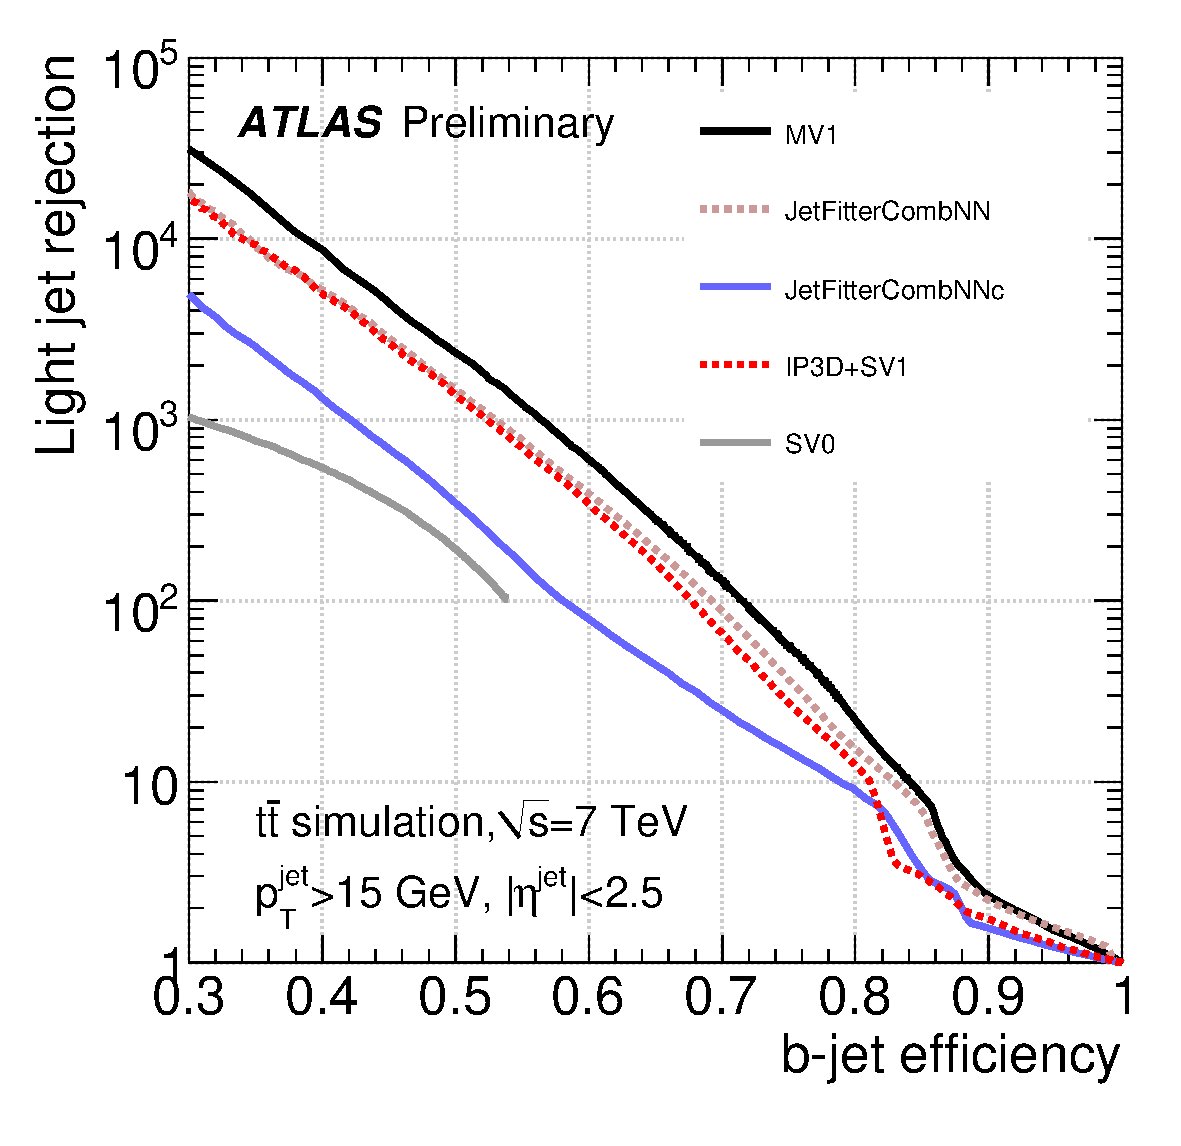
\includegraphics[width=0.45\textwidth]{mj/fig_01a.pdf}}
\subfigure[10q]{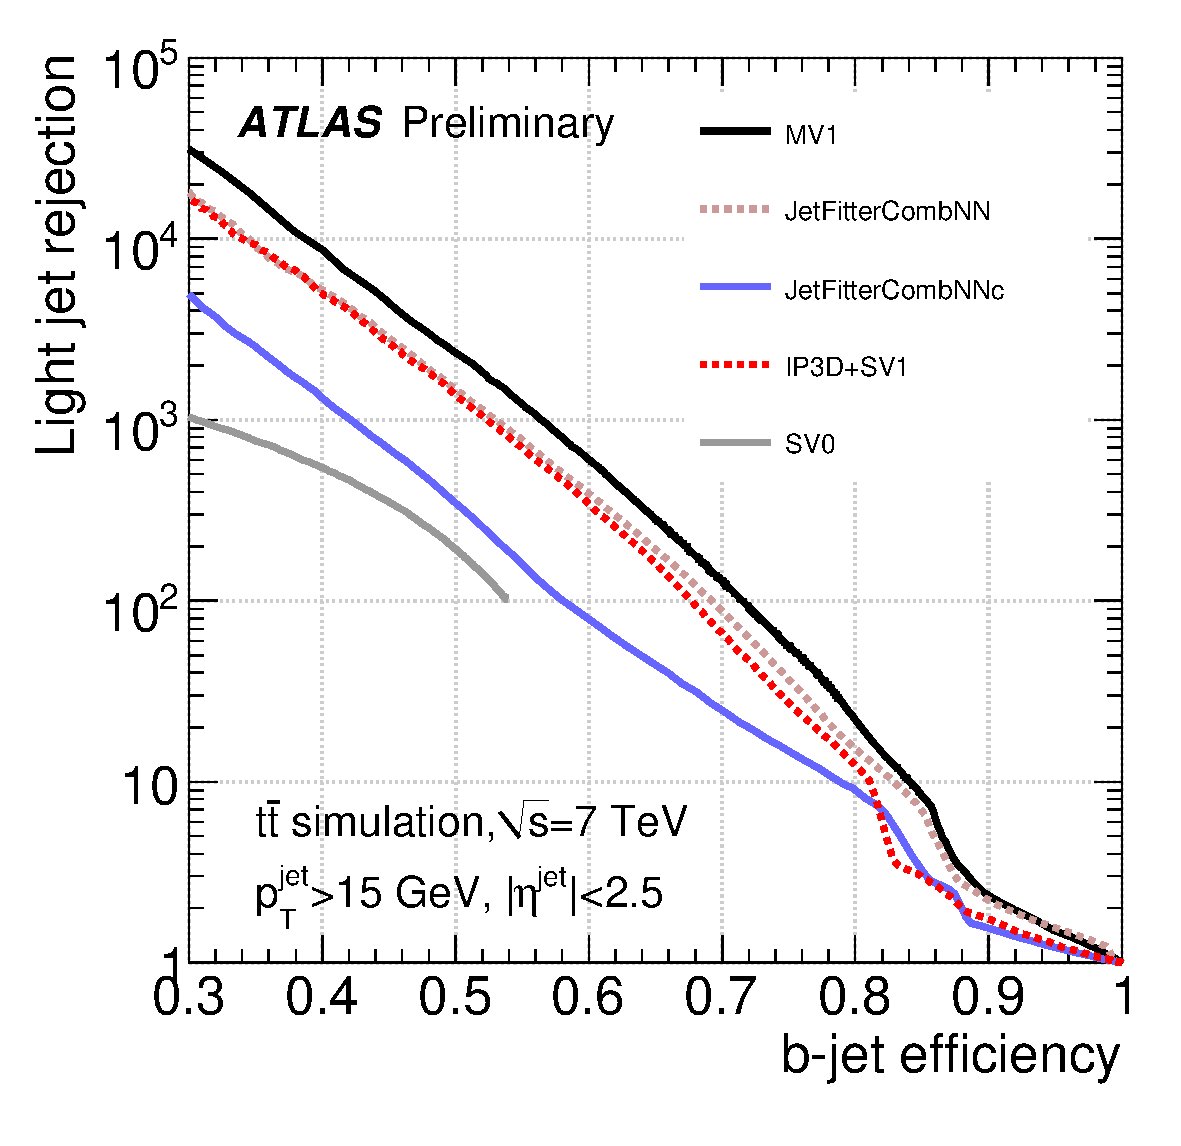
\includegraphics[width=0.45\textwidth]{mj/fig_01a.pdf}}
\label{fig:search:motivation:diagrams}
\caption{Feynman diagrams for a 6q and 10q final state with gluino pair production and RPV decays of the LSP. The 10q final state proceeds through an intermediate neutralino LSP.}
\end{figure}

%%%%%%%%%%%%%%%%%%%%%

Many different possibilities for the flavor structure of the quarks in this diagram exist. As discussed in Section~\ref{chapter:susy:r}, the  $\lambda''_{ijk}$ coupling is actually an anti-symmetric tensor which couples together one up type and two different down type quarks. This means, for example, that the \lsp can decay to a top-bottom-strange triplet, but not a top-bottom-bottom. The most generic assumption is to set all possibilities as equal, as a priori there is no preference for any particular combination. Moreover, there is an additional place for quark flavor to be decided, in the quarks coming from the gluino decay: these are set by the masses of the off-shell squarks in the theory. If the stop was very much lighter than the other squarks, for example, the gluinos would all decay through off-shell stops, leading to only tops from the gluino decays. Again, however, the most generic assumption is to set all squark masses to be degenerate (at 5 TeV, well above threshold), so all decays that are kinematically possible will happen. Ultimately, this means that in decay chains with many hadronically decaying top quarks can have up to 22 quarks in the final state, or as few as 10 in the case where no tops are included in the decays. 

Final states like these have largely been ignored because of the extremely difficult backgrounds: QCD multi-jet processes, which are usually suppressed by \met cuts, are dominant. The problem with a multijet background is actually two-fold. First, the extremely high cross-section requires very powerful variables to replace the \met cut in order to become sensitive. Additionally, the modeling of these backgrounds is also very challenging, generally requiring sophisticated data-driven techniques because of the inadequacy of MC simulation to model the high-multiplicity multijet final states.

An analysis searching for final states of this type is thus very attractive: SUSY could exist at rather low mass, and could be discovered if new analysis strategies and background estimation techniques were developed. Thankfully, jet substructure tools provide an answer to both elements of the problem. The following chapter describes a new search for RPV SUSY using jet substructure techniques, as published in \cite{RPVSUSY}. This is the first search for the 10-quark model previously described, and sets strong limits on the production of gluinos in all-hadronic final states.

%discuss final state structure, types of quarks, etc?

\section{Why Jet Substructure?}

The best way to understand the utility of jet substruture for this analysis is to consider an event display, as in Figure~\ref{fig:search:motivation:event-displays}. This display shows in the $y/\phi$ plane the \antikt $R=1.0$ Trimmed jets run on a background (left) and signal (right) event. Typically, analyses have used variables such as \Ht-- the sum of the transverse momentum of the jets-- to define a signal region. In this case, the \Ht of the two events is very similar, near $2$~TeV. However, the event on the right shows significantly more \textit{structure} in its jets than the event on the left: QCD jets are generally single-prong, while the jets in the signal have a richer topology.  

%%%%%%%%%%%%%%%%%%%%%

\begin{figure}
\centering
\subfigure[\herwigpp Dijet Background]{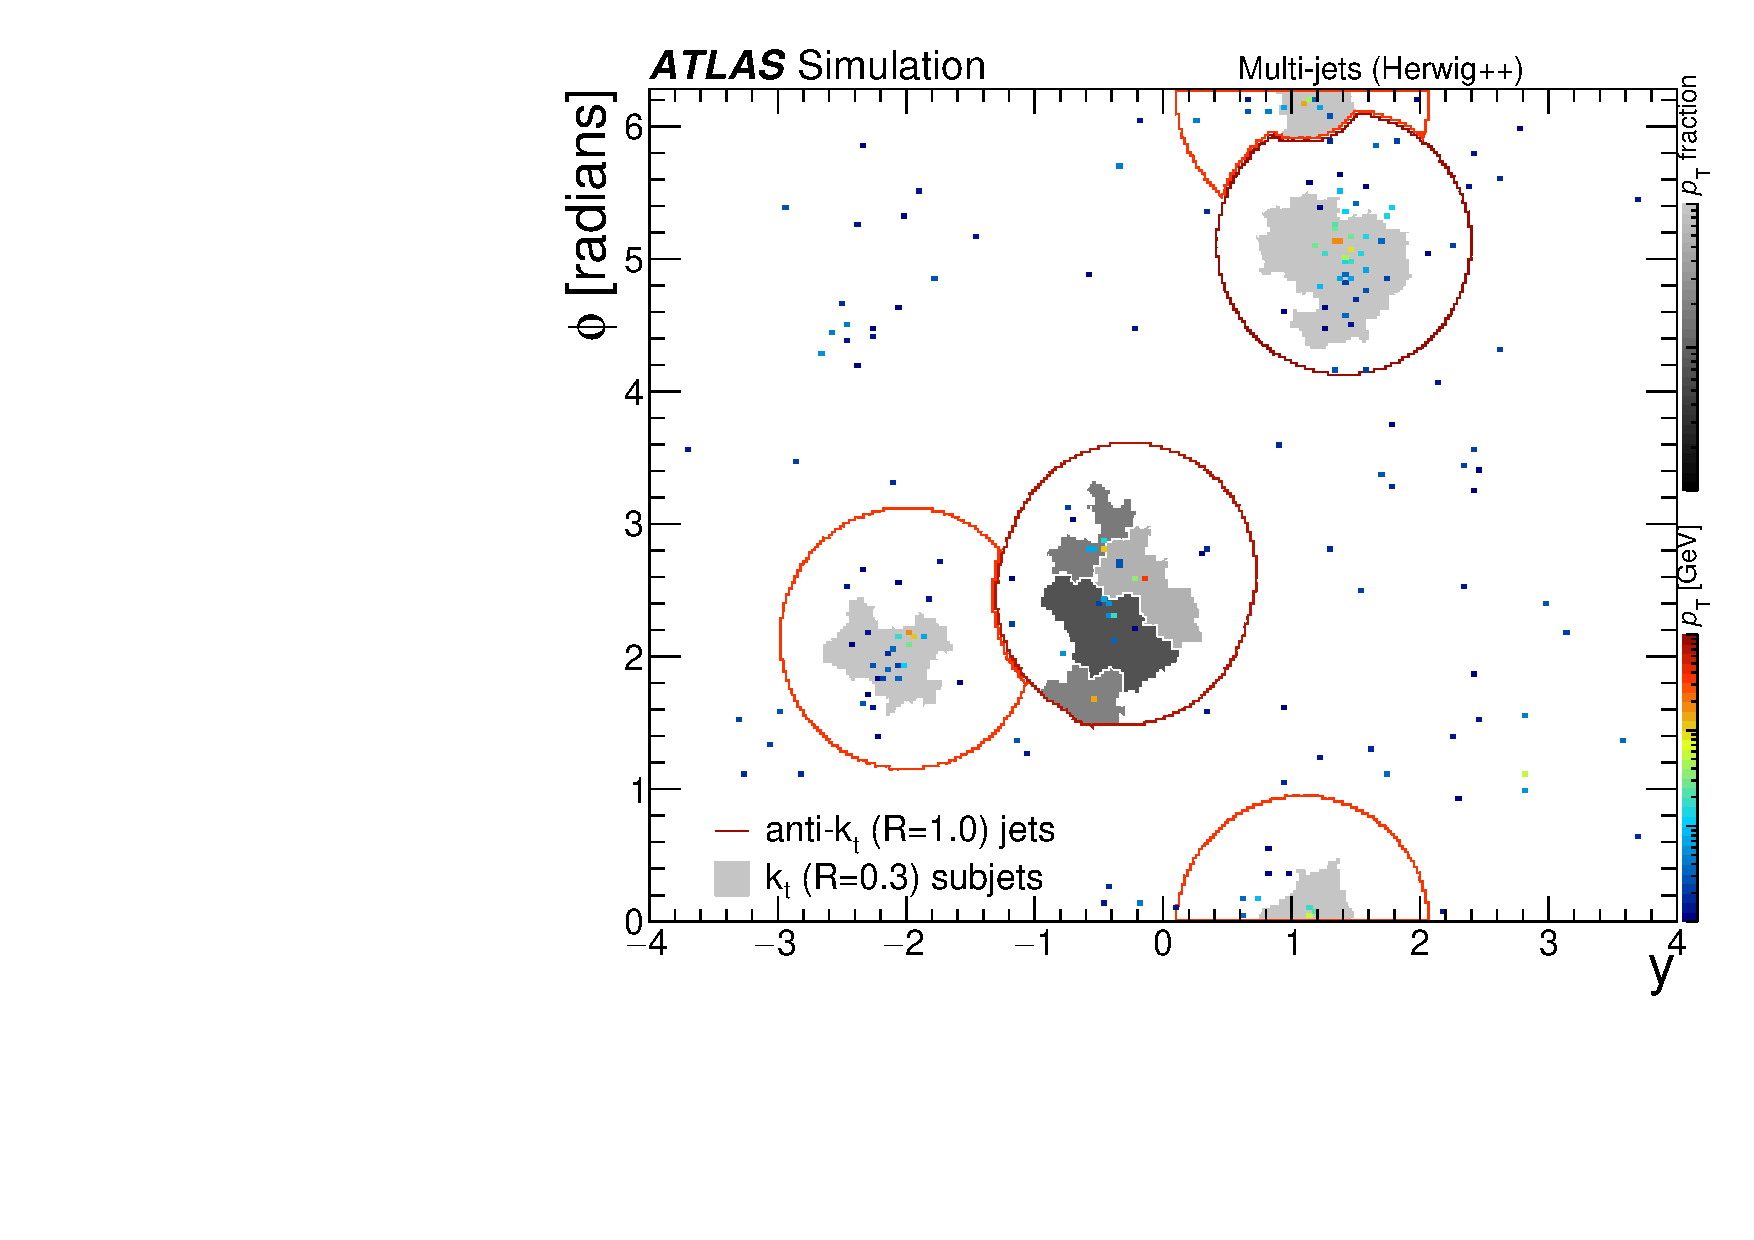
\includegraphics[width=0.45\textwidth]{mj/figaux_08f.pdf}}
\subfigure[\gl-\gl Signal]{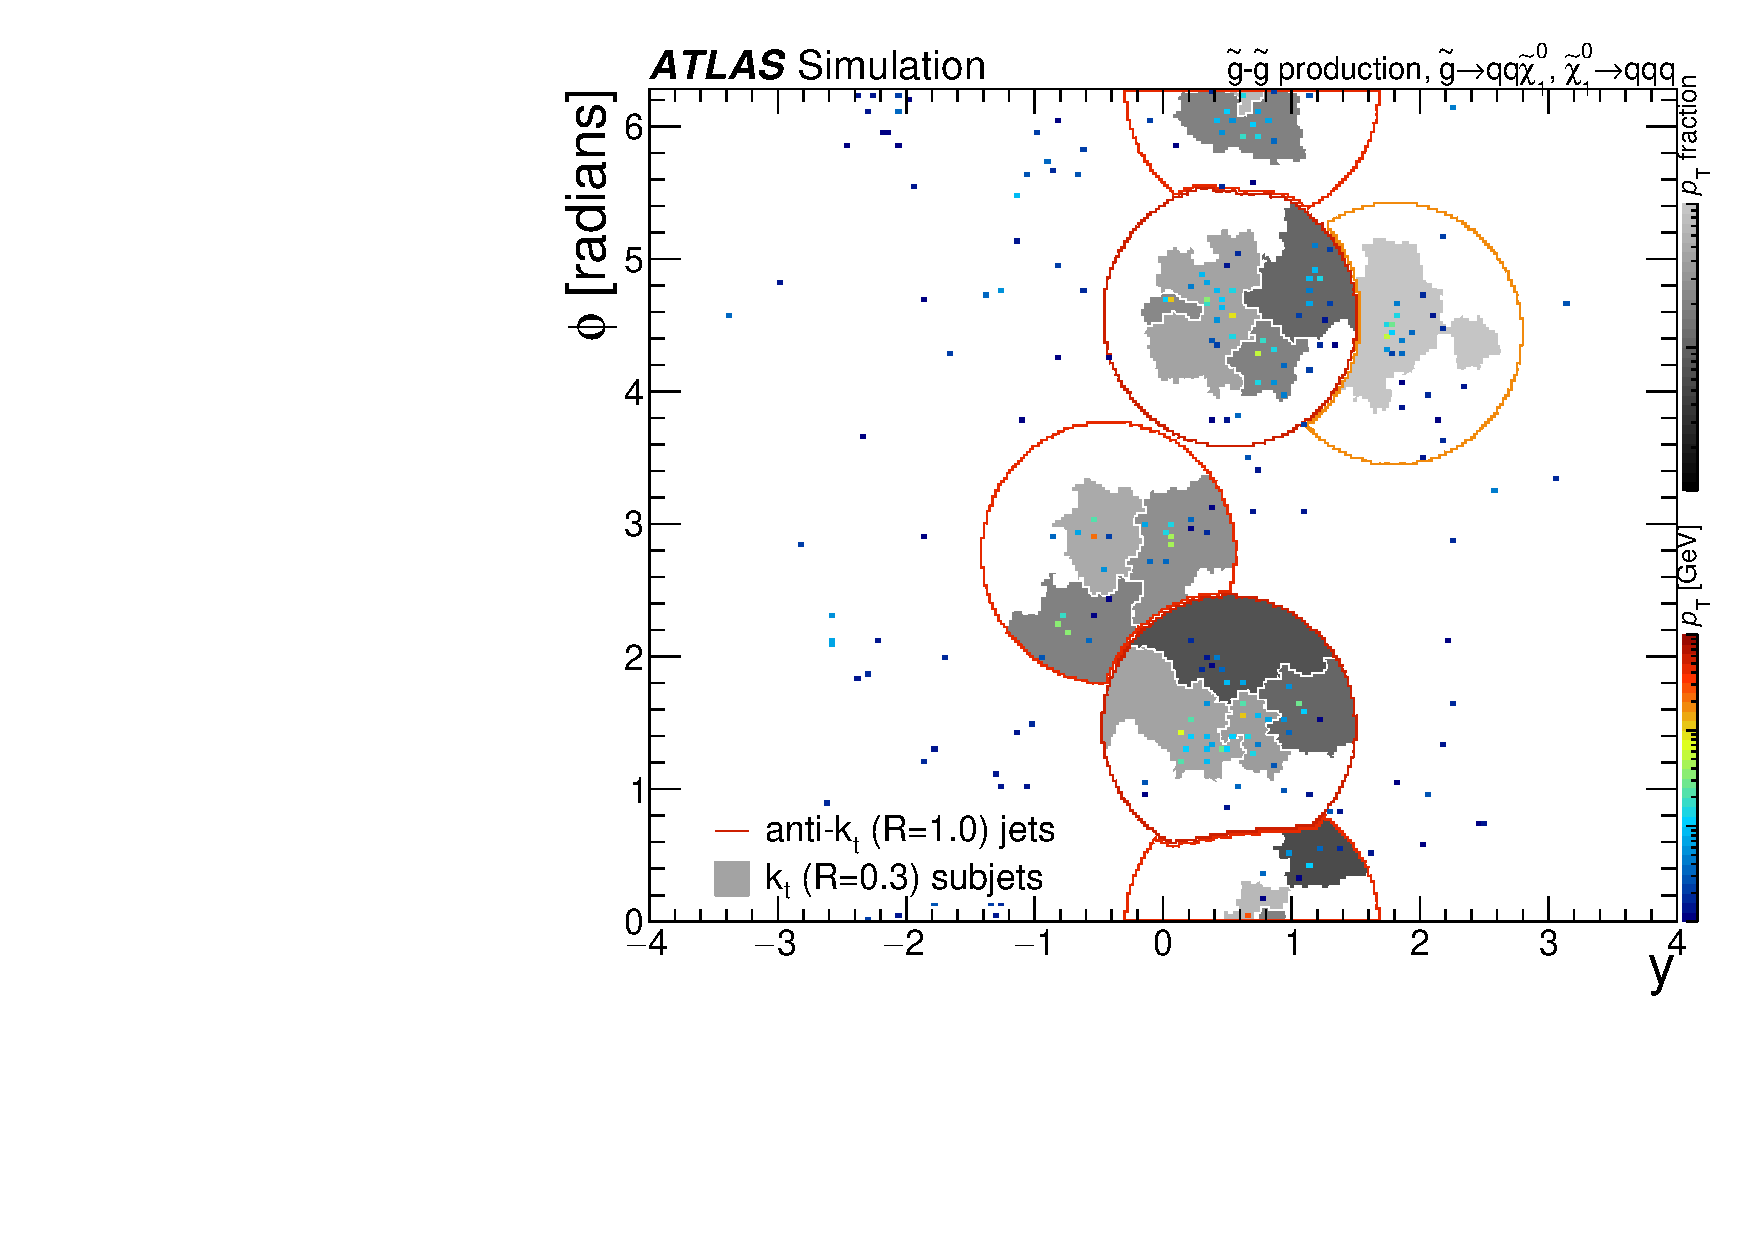
\includegraphics[width=0.45\textwidth]{mj/figaux_06f.pdf}}
\label{fig:search:motivation:event-displays}
\caption{Event displays for background and signal events with very similar \Ht (sum of jet \pt), but very different \textit{jet masses}.}
\end{figure}

%%%%%%%%%%%%%%%%%%%%%

Interestingly, these \largeR jets do not correspond to any particular top quark, or \lsp decay, or \gl decay products: the complicated, high multiplicity environment, along with relatively low \pt for quarks from the \lsp because of 3-body decays, means that most decays are not actually very collimated, and there is a great deal of overlap between quarks. All hope is not lost, however: instead of requiring mass windows, one can simply look for lots of structure. This approach is referred to as \textit{accidental substructure}: the quarks from various parts of the event accidently overlap in the \largeR jets used to reconstruct the event, and simply trying to identify ``lots of structure'' is sufficient to discriminate between signal and background. For this reason, analyses implementing this strategy generally require four \largeR jets in an event, and use the properties of these jets to search for new physics. \editnote{Cite me}

Thus, jet substructure provides a path to discrimination between signal and background, which will be discussed further in Section~\ref{chapter:search:substructure:mj}. Jet substructure actually provides a path for background estimation as well: the \textit{expected structure} of QCD can be measured in control regions and extrapolated to a signal region. This strategy is discussed in Section~\ref{chapter:search:substructure:templates}. \editnote{Cite me}

\subsection{Total Jet Mass, and Other Variables}
	\label{chapter:search:substructure:mj}

A variable like \Ht (or \met) is convenient for analysis because it reduces the complexity of the event to a single scalar variable which quantifies the total energy (or missing energy) in an event. Using this approach as in inspiration, it is also possible to create variables which describe not the amount of energy, but the amount of structure in an event. \editnote{Cite all of me} The simplest possibility is called the \textit{Total Jet Mass}, and is defined as:
%
\begin{equation}
\MJ = \sum_{i=1}^4 M_J^i,
\end{equation}
%
where $i$ iterates over jets with some \pt and $|\eta|$ thresholds (typically 100 GeV and $2.5$ respectively, though the exact \pt cuts on the jets depend on the trigger and signal points, as described in Section~\ref{chapter:search:search}). The $\njet$ requirement is usually set to $\geq 4$.  This \MJ variable is expected to be rather sensitive to the signal: the \largeR jets in a \gl-\gl event are expected to be composed of many quarks each, and thus each have substantial mass compared to dominantly single-prong QCD backgrounds. In Figure~\ref{fig:search:motivation:event-displays}, for example, the background has $\MJ = 260$~GeV, while the signal has $\MJ = 705$~GeV: a substantial difference, even though the \HT is very similar!

There are many other similar variables which can be composed using the structure of the \largeR jets. For example, the \textit{Event-Subjettiness} is defined as:
%
\begin{equation}
T_{MN} = \left(\prod_{i=1}^4 \tau_{MN}\right)^{1/4}.
\end{equation}
%
This is the geometric mean of the n-subjettiness ratios of the leading four jets: the variable is designed to distinguish to search for compatibility of an $M$-prong structure, compared to an $N$-prong, where $M>N$. Typically $M=3$, $N=2$ and $M=2$ and $N=1$ are studied.

Another potentially useful variable is \textit{subjet counting}:
%
\begin{equation}
N_\mathrm{X}^\Sigma = \sum_{i=1}^4 N_\mathrm{X}^J,
\end{equation}
%
i.e. the total number of sub-jets (defined with some algorithm $X$) in the leading four jets in the event~\cite{SubjetCounting}. The number of subjets is again expected to be strongly discriminating: for signal, it should be approximately equal to the number of quarks in the final state, and for background it should be much lower (approximately equal to one subjet per jet). Many different algorithms are possible for defining the subjet algorithm, but two particularly well optimized choices seem most promising~\cite{SubjetCounting}, referred to as the \kt and \ca (though the clustering algorithms are far more involved than the algorithms previously defined). In general, the \kt-counting technique looks for subjets with differing \pt, while the \ca-counting looks for more balanced \pt distributions (following the asymmetry cuts in the original BDRS algorithm~\cite{BDRS}). 

Finally, there are also more kinematic variables which can be constructed from the event (as opposed to the previously discussed structure-based variables). One particularly powerful variable is the difference in pseudo-rapidity between the leading two jets:
%
\begin{equation}
\Delta \eta = |\eta_J^1 - \eta_J^2|.
\end{equation}
%
Supersymmetry is produced in $s$-channel processes, which are generally more centrally produced, and therefore have small $\Delta\eta$, whereas QCD also contains many $t$- and $u$-channel processes which have more forward production, and thefore a very high $\Delta\eta$. It is also possible to define $\Delta y$, the difference in absolute rapidity, but the performance in the two variables is essentially identical.

One last set of variables which can potentially be useful are various ways of using the \pt of the third leading jet, $\pt^3$. Generally multi-jet backgrounds are dominated by di-jet like topologies, where the third jet has relatively low \pt compared to the leading two jets which dominate the event: signal, on the other hand, should have a more even \pt distribution, and therefore a higher $\pt^3$ than background. Likwise, one can look at the ratio $\pt^3/\pt^1$, which normalizes the third \pt by the first. The \pt distributions between signal and background are generally very similar, but in combination with many of the other mass cuts, this can be a useful pre-selection device. 


\subsection{Jet Mass Templates}
	\label{chapter:search:substructure:templates}

The second important aspect of jet substructure in the analysis is in the measurement of the background. Because the main discriminating variables are composed of the \textit{structure} of jets, and the kinematics of these events are less sensitive to new physics, one can form a background prediction based on the structure of jets in a signal-depleted control region, and use the kinematics as a transfer factor into a signal region. These measurements in the control region are formulated as \textit{jet substructure templates}, and are defined in detail in \cite{MassTemplates}. Figure~\ref{fig:search:substructure:template-big-picture} summarizes the procedure: the template, constructed from the training sample, is convoluted with the kinematics of the signal sample, produced a Dressed Sample, which is a distribution of a substructure variable usable for the background estimate.

%%%%%%%%%%%%%%%%

\begin{figure}
\centering
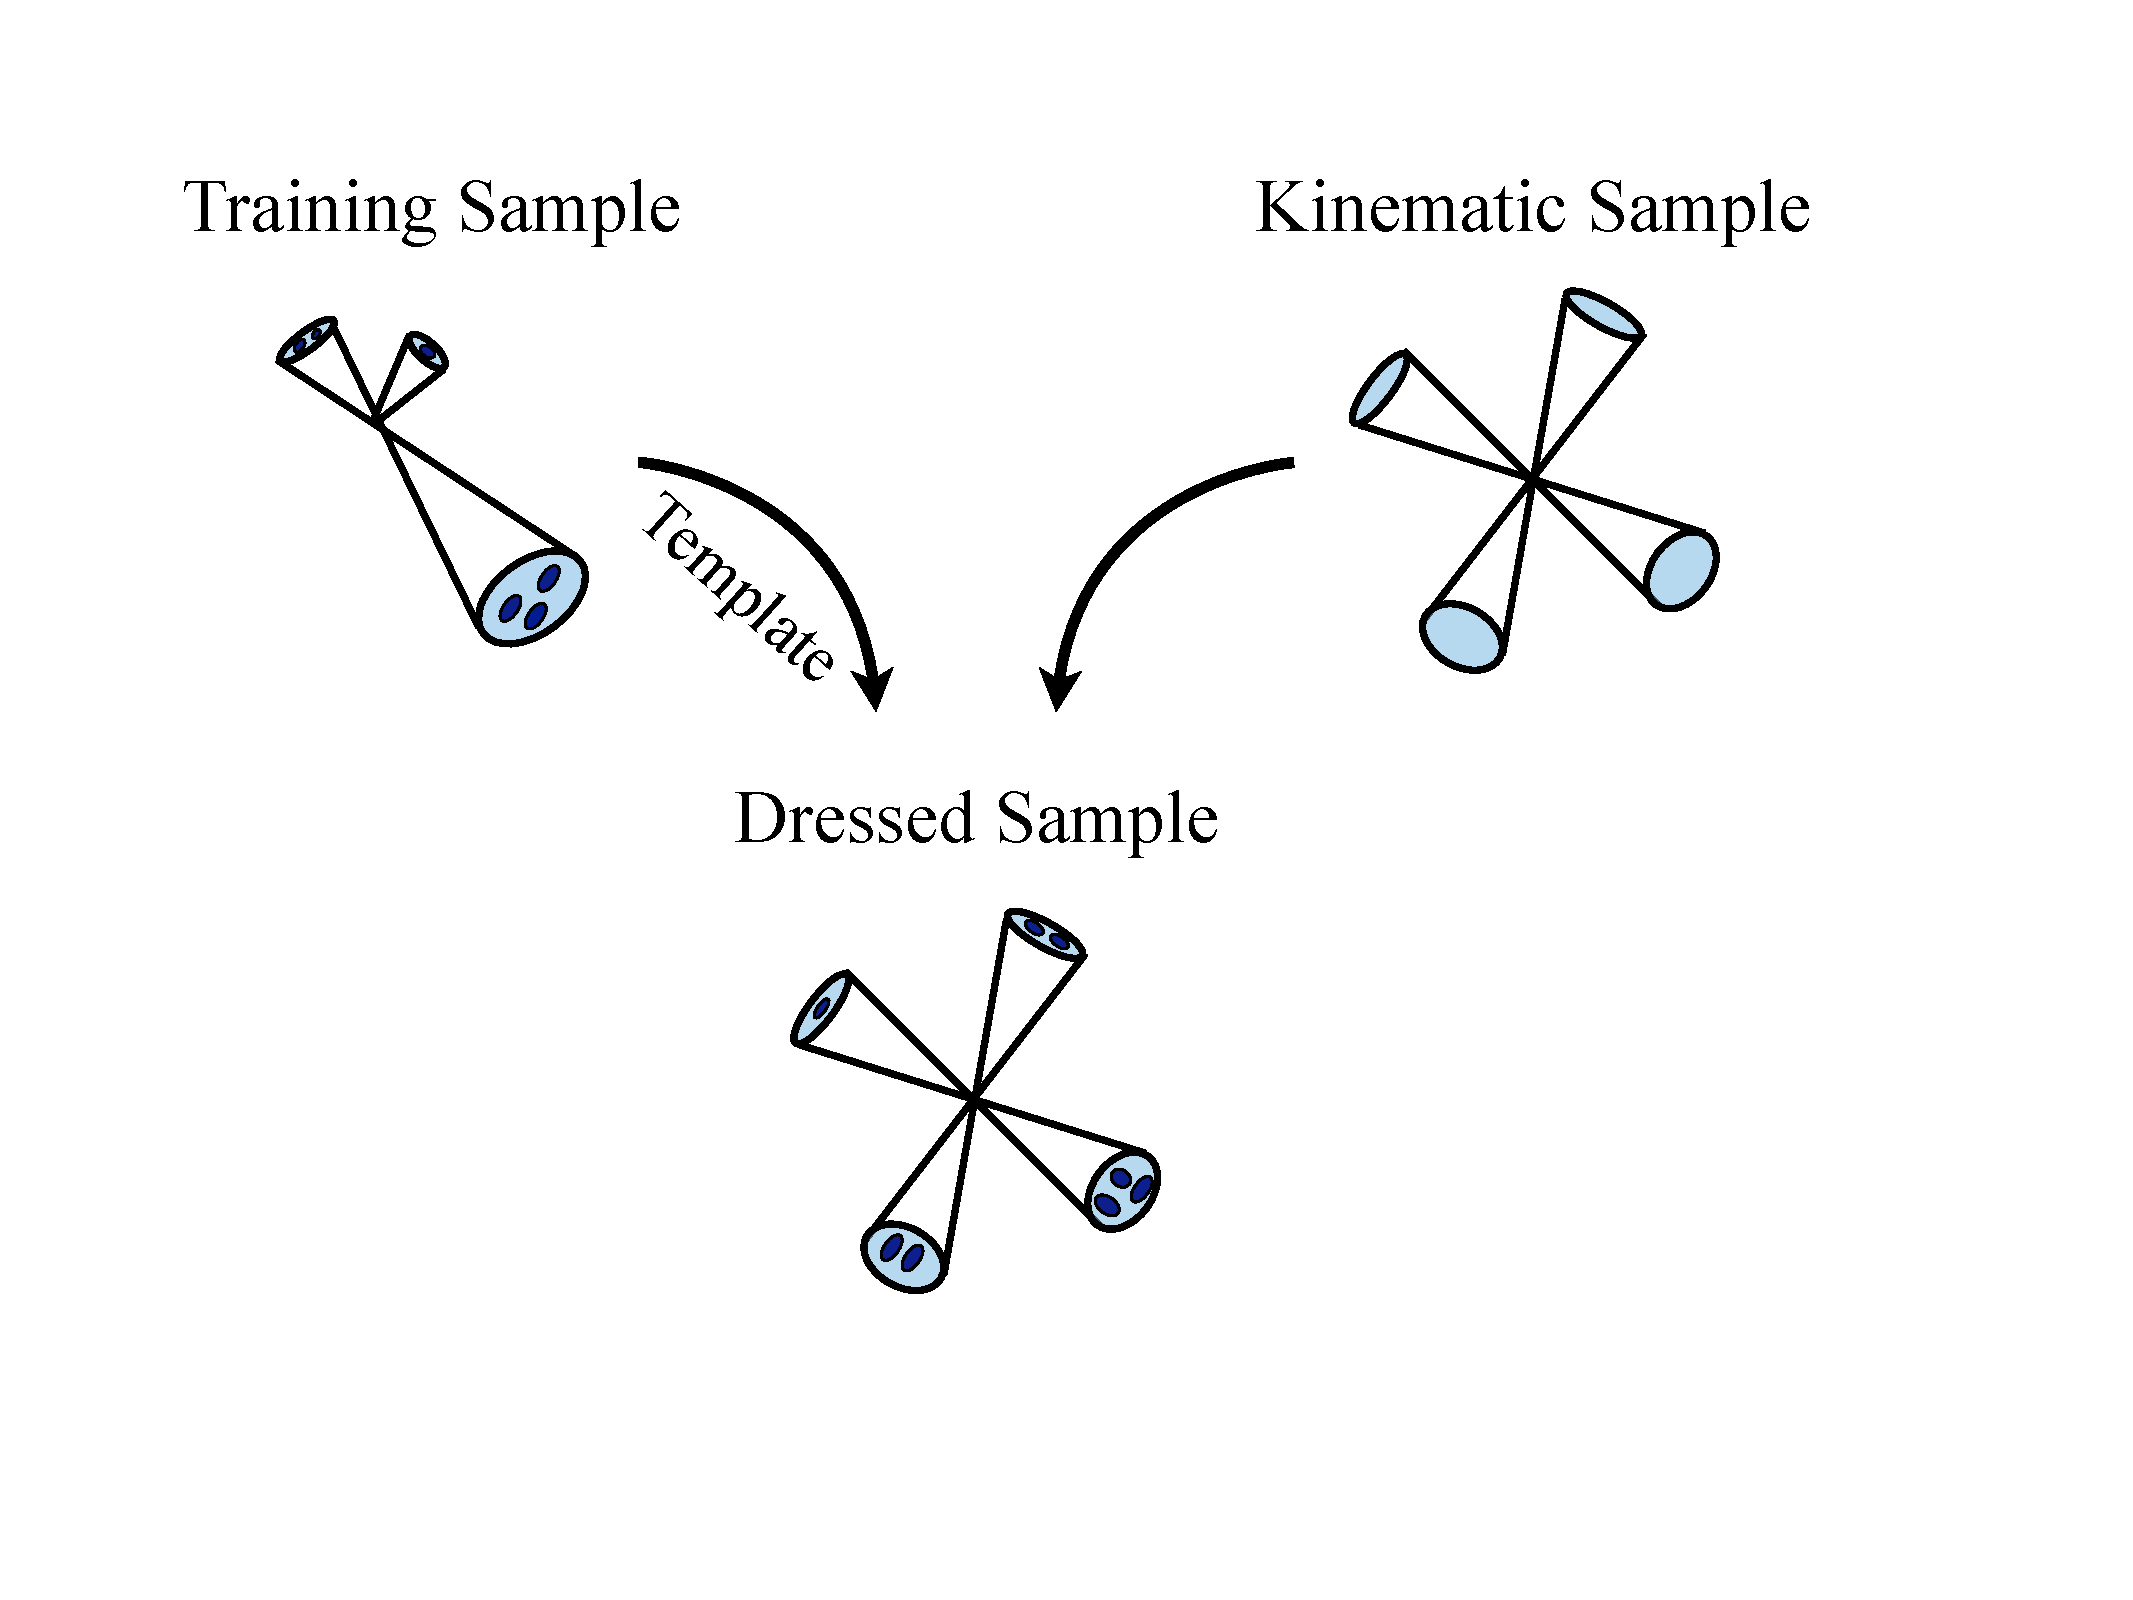
\includegraphics[width=0.7\textwidth]{INT/BigPictureSketch}
\label{fig:search:substructure:template-big-picture}
\caption{The strategy used to develop background estimates using jet substructure templates.}
\end{figure}

%%%%%%%%%%%%%%%%   

The background strategy can be formally described as follows. First, we consider $J_{ij}(z)$, which is a $D$-dimensional vector of variables $z$, which can be ``inputs'' (i.e., kinematic variables like \pt or $\eta$) or ``outputs'' (i.e., substructure variables like mass or $\tau_{21}$), and where $j$ is indexed over events and $i$ for jets in each event. One can define a histogram $T_i = \{J_{i1}, J_{i2}..., J_{iN_T}\}$, which is the multi-dimensional distribution of the variables $z$ defined separately for each jet $i$. To increase statistics, various sums over $i$ can also attempted (for example, using the leading and sub-leading jets together). When $T$ is normalized, it represents a probability distribution function for the jet $i$ to have various properties. However, as this is a highly multi-dimensional object, there can be various regions of this function which are not filled by the training sample, but which are still important for the background estimation. The histograms are therefore smoothed using a Gaussian kernel method, which produces the final templates. In particular, the smoothed template for each jet $i$ is:
%
\begin{equation}
\hat{\rho}_i(z) = \frac{1}{N_T} \sum_{J\in T_i} K_h(z - z_J)
\end{equation}
%
where $K_h$ is the smoothing kernel term, defined as:
%
\begin{equation}
K_h(z) = \frac{1}{(4\pi)^{D/2} \det h} \exp \left[ - \left(h^T h \right)^{-1}_{ij} z^i z^j \right]
\end{equation}
% 
where $h$ is a matrix which describes the width of the kernel. Thus, the template is nothing more than the sum of the multi-dimensional smoothed Gaussians formed by every point in the training. The last point is determining the exact form of the matrix $h$. Usually the best choice is defined by the ``Asymptotic Mean Integrated Squared Error'', which is:
%
\begin{equation}
h_{ij}^\mathrm{amise} = c \hat{\sigma}_{ij} N_T^{-\frac{1}{D+4}}
\end{equation}
%
where $c$ is an $O(1)$ constant, and $\hat{\sigma}$ is the estimate of the square root of the covariance matrix for $\rho(z)$ (the true distribution). For the analysis below, $c=0.01$ is typically used. A schematic diagram summarizing the technique is shown in Figure~\ref{fig:search:substructure:smoothing}

%%%%%%%%%%%%%%%%

\begin{figure}
\centering
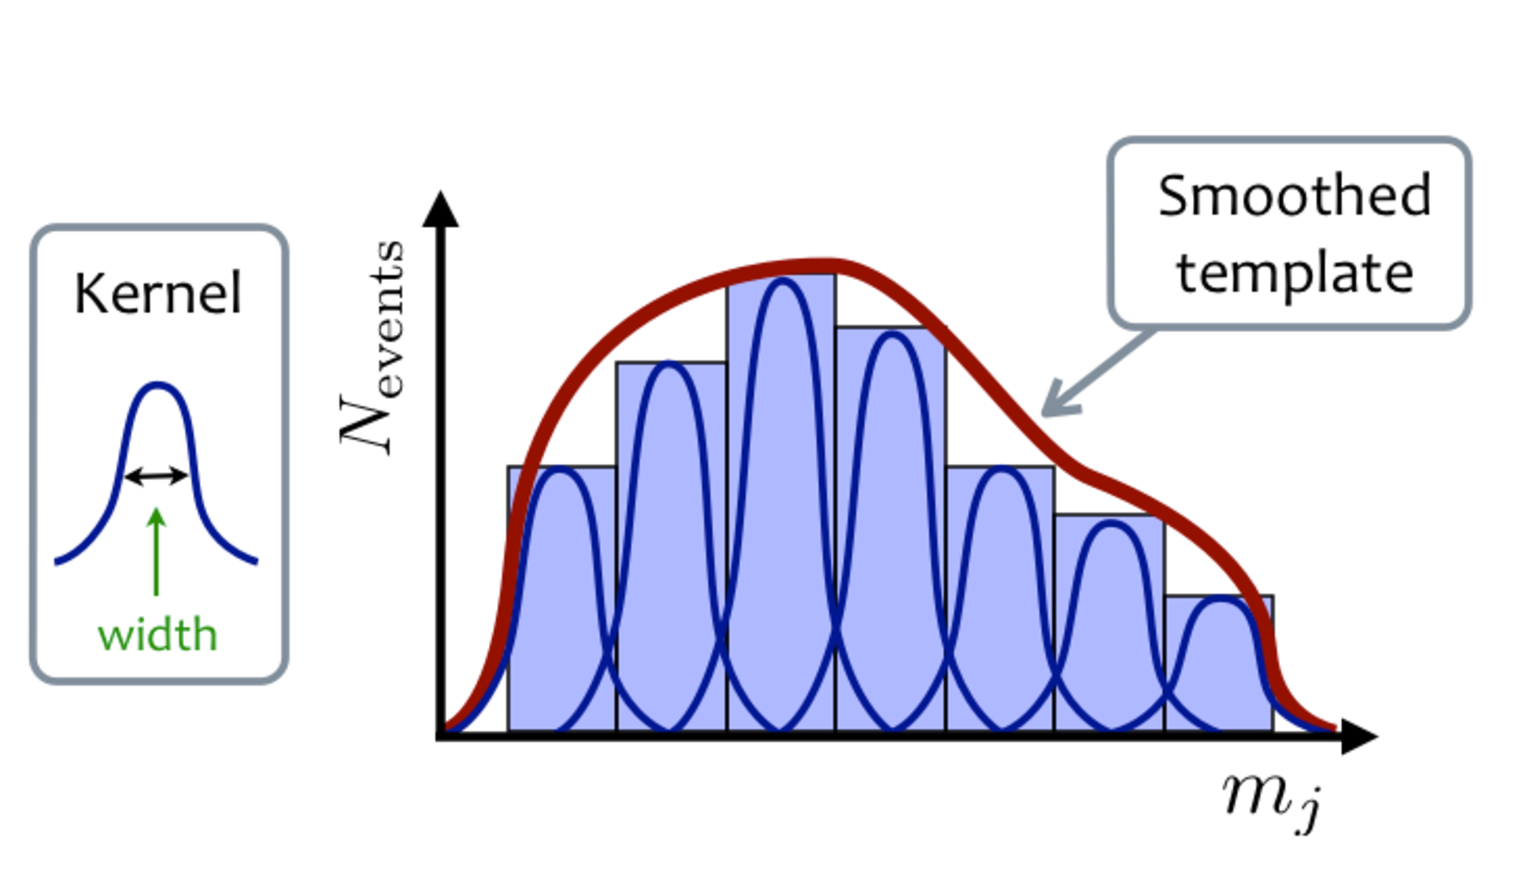
\includegraphics[width=0.7\textwidth]{INT/KernelSmoothing}
\label{fig:search:substructure:smoothing}
\caption{A schematic describing the use of the Gaussian Kernel smoothing method to generate a smoothed template.}
\end{figure}

%%%%%%%%%%%%%%%%  

There are two sources of error due to this smoothing: the \textit{bias} and the \textit{variance}, defined as:
%
\begin{align}
b(z) &= \rho(z) - \hat{\rho}(z)\nonumber\\
v^2(z) &= \langle \hat{\rho(z)}^2 \rangle  - \langle \hat{\rho}(z) \rangle^2.
\end{align}
%
There is also a potential error due to  physics: the extrapolation from a control region to a signal region may not be fully controlled by the kinematic distributions. This is discussed in more detail in Section~\ref{chapter:search:search:background}. 

The bias is an important potential source of error: by definition, it is exactly the difference between the true distribution and the estimate. If we can find an estimate for the bias, we can even correct for this error immediately and derive an improved estimate. In fact, such an estimate can easily be derived by smoothing again the smoothed distribution: this is accurate to first order in $h$ (as shown in detail in Appendix A of \cite{MassTemplates}). The twice smoothed template is:
%
\begin{equation}
\hat{\hat{\rho}}(z) = \int d^D z' \hat{\rho}(z') K_h (z-z')
\end{equation}
% 
and so the bias estimator is:
%
\begin{equation}
\hat{b}(z) = \hat{\hat{\rho}}(z) - \hat{\rho}(z).
\end{equation}
%
This in turn defines the bias corrected template:
%
\begin{equation}
\hat{\rho}^*(z) = \hat{\rho}(z) - \hat{b}(z).
\end{equation}
%
This is the final template (actually, the median of a set of toys of such templates) used for the background estimate. The full difference between the corrected and the un-corrected term (i.e., the full size of $\hat{b}(z)$) is used as a systematic error in the analysis.

Before describing the estimate of the variance $v^2$, we can define how the template $\hat{\rho}^*(z)$ is used to generate a background prediction. In particular, we want to understand the distribution of the substructure variables $x$ as a function of the kinematic variables $k$, which were previously concacted into one vector $z$. Currently, we have a joint probability distribution $\hat{\rho}^*(x,k)$, but we want a \textit{conditional} probability distribution $\hat{\rho}^*{x|k}$. This is derivable as:
%
\begin{equation}
\label{eqn:templates:conditional}
\hat{\rho}^*{x|k} = \frac{\hat{\rho}^*(x,k)}{\hat{\rho}^*(k)} = \frac{\hat{\rho}^*(x,k)}{\int d^d x' \hat{\rho}^*(x',k)} 
\end{equation}
%
where $d$ is the number of kinematic variables in $k$, and $\hat{\rho}^*{x|k}$ defined such that the integral over $x$ is normalized to 1. The remaining question is how to do the non-trivial integral in the denominator of Equation~\ref{eqn:templates:conditional}. One simple solution is to perform the integral using a Monte Carlo approach: each possible value of $x$ (sampled across the full domain of the variable with 500,000 steps, each referred to as $\alpha$) is evaluated simultaneously with the kinematics $k$, returning a weight $w_\alpha$ (or $w^*_\alpha$ for the bias-corrected template) for such a combination. Thus, every kinematic event $k$ creates a distribution for the substructure variables $x$ which is compatible with those kinematics, and this distribution is normalized to 1 (the weight of the particular kinematic event is in total 1). To combine the templates of multiple jets, the product of these weights is computed, as the convolution of the probability density functions of each jet gives the combined probability. For example, for a given event with jet kinematics $k_1$ and $k_2$, one could calculate $M_1 + M_2 = \{w^*_{\alpha,1} w^*_{\alpha,2}\}$, i.e. creating a histogram for the variable $M_1 + M_2$ filled with the product of all the weights; this histogram could then be used to fill another histogram for every event $j$, giving a combined distribution of $M_1 + M_2$ for all the kintematic events in the analysis. This histogram is normalized correctly to the number of events in the dataset: a cut on $M_1 + M_2$, either creating mass windows or a simple cut-and-count region, can be compared directly to the observed mass distribution to search for new physics.

There is on subtlety to this point: if new physics is present, then the ``extra'' events from new physics would be included in the normalization-- and so would pass undetected in the inclusive distribution. However, if the \pt of new physics and QCD is the same, the bulk of the `predicted' masses would fall in the low mass range, near the peak of QCD-- the tails would see a very small, sub-percent, additional contribution (as they are a factor of a million or lower compared to the peak in QCD). Thus, the standard interpretation of a background prediction, with a signal appearing as an additive excess, is reasonable in the tails of the mass distribution, even though the overall normalization would be preserved (and so in the case of an observation of new physics, the peak would see a slight under-prediction of the mass). The technique in \cite{MassTemplates} avoided this issue by using normal MC simulation, normalized to luminosity, to create the kinematic sample used to create the background prediction: however, as multi-jet \pt spectra are notoriously difficult to normalize, and using an MC simulation would add JES related systematics, a data-only technique is used by this analysis.

Finally, the direct analytical calculation of the variance is very difficult, but a different straightforward technique is easy to apply. \textit{Bootstrapping}-- i.e., generating toys via varying the number of events in each bin in the histogram $T_i$ via the Poisson distribution cenetered at the bin value, performing the same procedure on all the toys, and calculating a new final histogram for each toy. Then, each mass bin of interest can assessed by the full ensemble of these toy histograms: the median is used as the nominal value, and the $\pm 1\sigma$ values (i.e., the 68th and 32nd sorted entries when using 100 toys) are used to bracket the derived variance. This corresponds to the statistical uncertainty of the templates. Note that because the variance computed in this way is exact (up to fluctuations based on the number of toys) while the bias is a first order approximation, typically $c$, the constant in the rule-of-thumb, is selected to \textit{undersmooth}: this raises the size of the variance (which we know very well) and lowers the size of the bias. In the limit that the variance dominates, higher order corrections to the bias estimation do not matter.

Thus, by measuring jet properties (such as the mass, or the n-subjettiness) as a function of the kinematic variables using mass templates, one can use jet substructure as a background estimation technique. In this sense, jets are used as a tool to divide up the event, and characterize the expected properities of portions of the detector.
%

\section{Constructing a Search}
\label{chapter:search:search}

\subsection{Optimization}
\label{chapter:search:search:optimization}

While the complicated multi-jet backgrounds generally require the previously discussed data-driven background techniques to create reliable predictions for the final analysis, it is cumbersome to use these techniques for performing the optimization over a large number of possible variables. For this reason, we use signal MC and \herwigpp di-jet MC to explore the previously defined variables, and to select the most useful way of defining the analysis. The goal is to find two variables which are \textit{uncorrelated}: that is, that they provide discrimination power more or less independently of each other. In this way, one variable can be used to define signal and control regions, while another can be used as the final cut in the signal region to define the precise search region.

One initial question is the number of jets required in the signal region, and which jet algorithm to use. The jet algorithm is the \antikt $R=1.0$, built from locally calibrated topological clusters, with trimming of $\Rsub = 0.3$ and $\fcut > 5\%$, as described in Chapter~\ref{chapter:jet-reconstruction}. These jets are available to 100 GeV: below this point, the calibrations and uncertainties are not valid. An initial optimization found that requiring $\geq 4$ jets above this threshold was the most effective strategy: exactly 3-jet and lower multiplicities are background dominated, while the signal efficiency for a $> 5$ is rather low. Note that the requirement on 4 jets is inclusive: jets with higher multiplicity are allowed. It should also be noted that jets are required to fall with $|\eta| < 2.5$, the region of validity of the systematic uncertainty measurement: jets outside of this requirement are not considered, so the ordering of the 4 jets in the analysis takes into account only jets within this proper fiducial region.

\subsubsection{1D Optimization}

Figures~\ref{fig:search:search:optimization:HT}, \ref{fig:search:search:optimization:MJ}, \ref{fig:search:search:optimization:T21}, \ref{fig:search:search:optimization:T32}, \ref{fig:search:search:optimization:NCA}, \ref{fig:search:search:optimization:NKT}, \ref{fig:search:search:optimization:PT31}, and \ref{fig:search:search:optimization:DEta} show the distribution of a given variable for both signal (in colors) and background (in black) on the left, while the right shows the signal efficiency vs. background rejection (defined as 1/(background efficiency)). Several trends are clear for most of the variables: higher \mgluino raises the energy of the event and increases the discrimination power of most of the variables. Some variables have less dependence on this, however, such as $T_{21}$ and $T_{32}$.

%%%%%%%%%%%%%%%%%%%%%

\begin{figure}
\centering
\subfigure{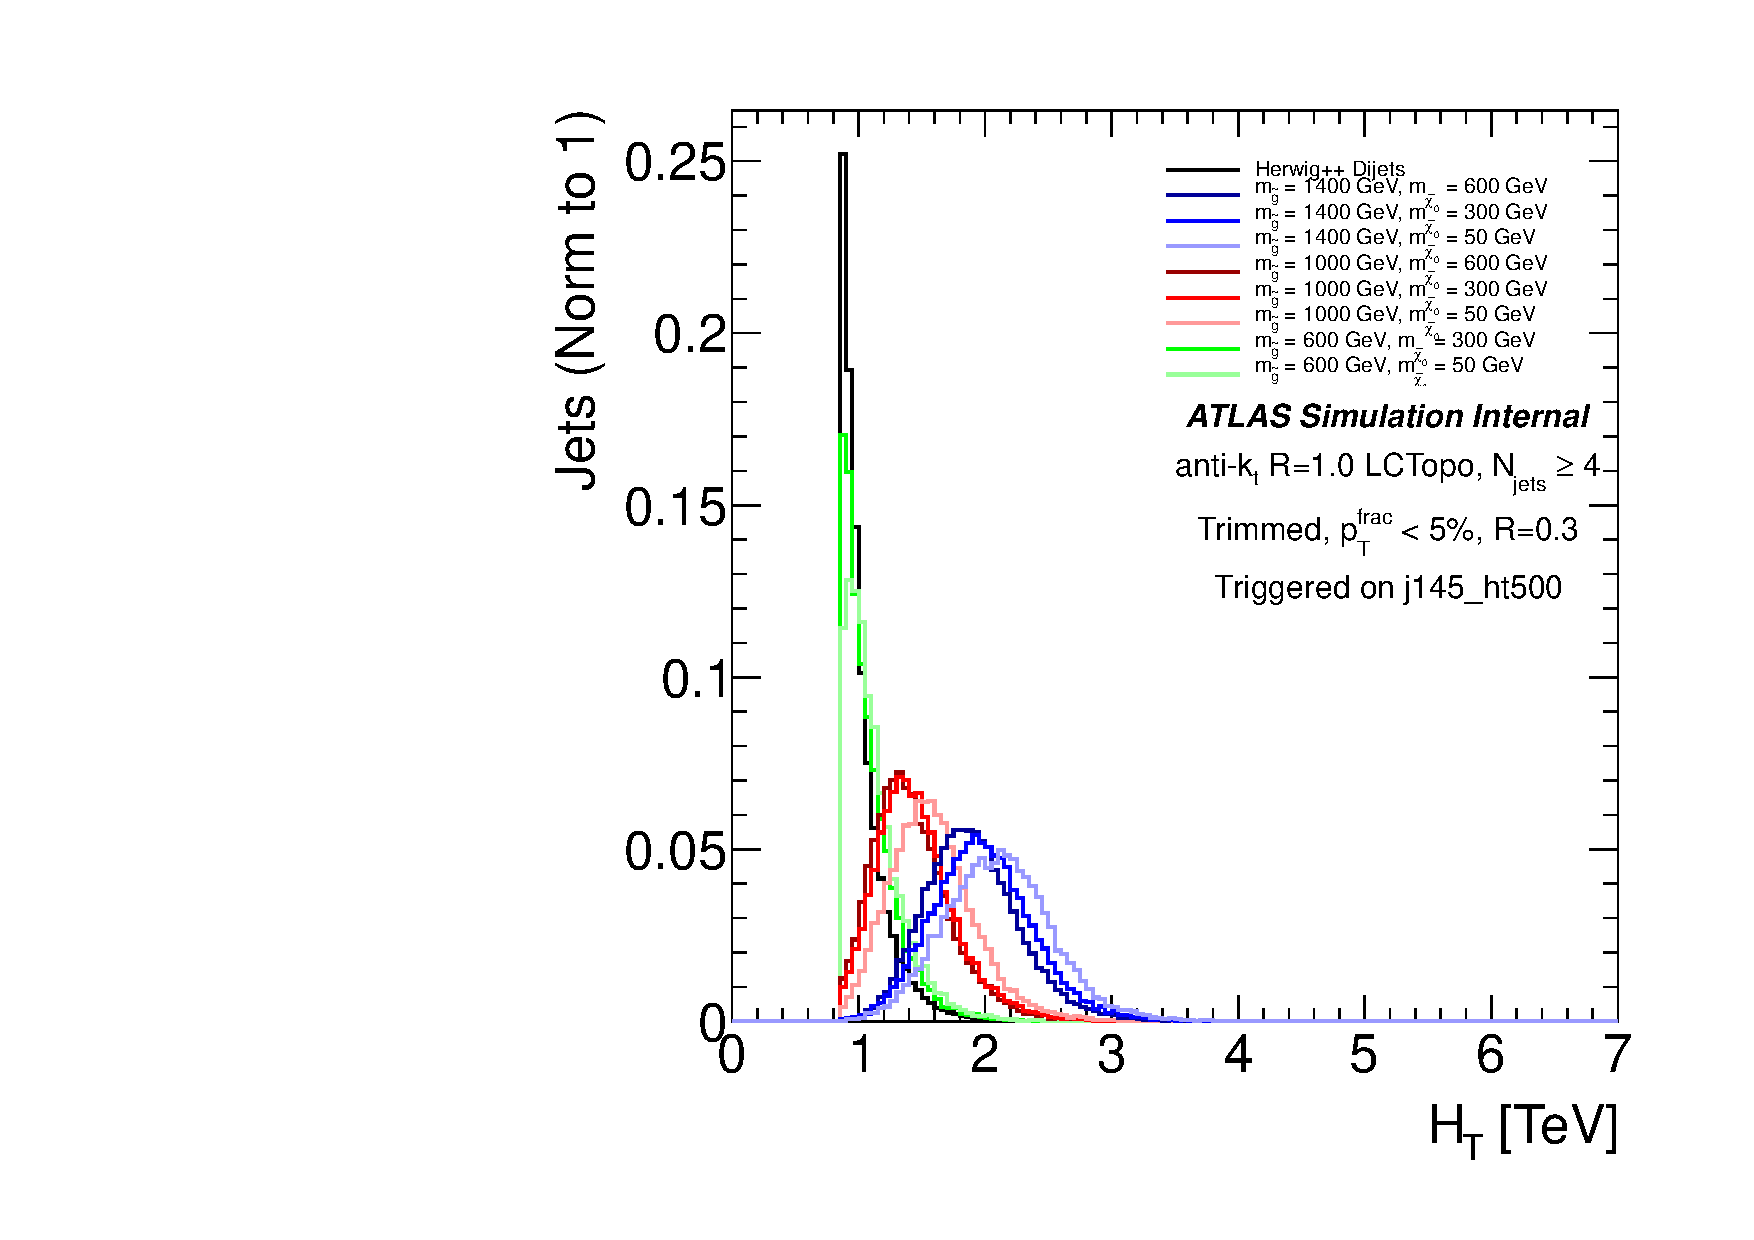
\includegraphics[width=0.45\textwidth]{INT/AntiKt10LCTopoTrimmedPtFrac5SmallR30_j145_ht500_NjetIncl_NFatJetMin4_HT4_RPVGluino.pdf}}
\subfigure{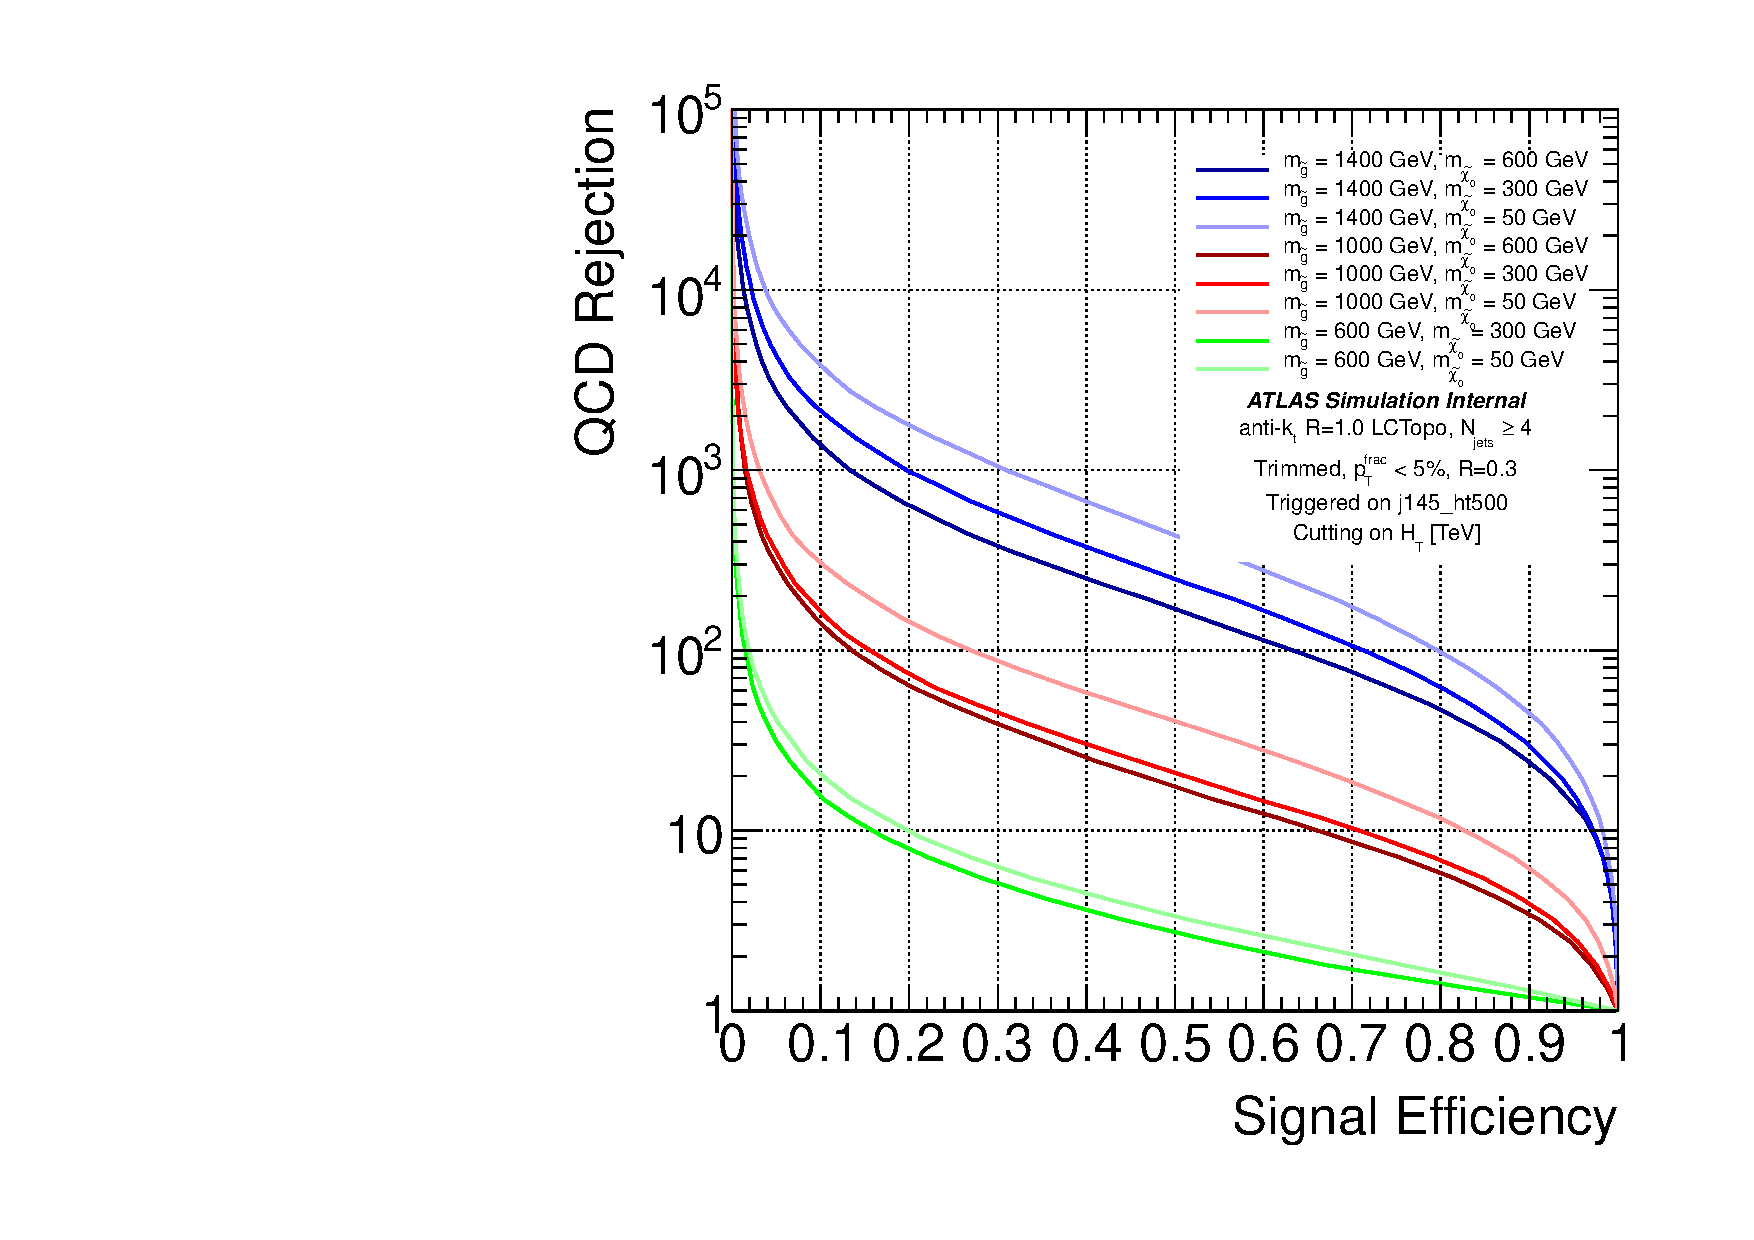
\includegraphics[width=0.45\textwidth]{INT/AntiKt10LCTopoTrimmedPtFrac5SmallR30_j145_ht500_NjetIncl_NFatJetMin4_HT4_g_RPVGluino}}
\label{fig:search:search:optimization:HT}
\caption{Distribution of $H_T = \sum_{i=1}^4 \pT^J$, a typical variable used to measure the energy in an event and discriminate between signal and background. Several signal mass points and the \herwigpp di-jet background are shown. The right-hand plot shows the signal efficiency vs. background rejection of a scan of possible cuts on the \HT distribution.}
\end{figure}

%%%%%%%%%%%%%%%%%%%%%


%%%%%%%%%%%%%%%%%%%%%

\begin{figure}
\centering
\subfigure{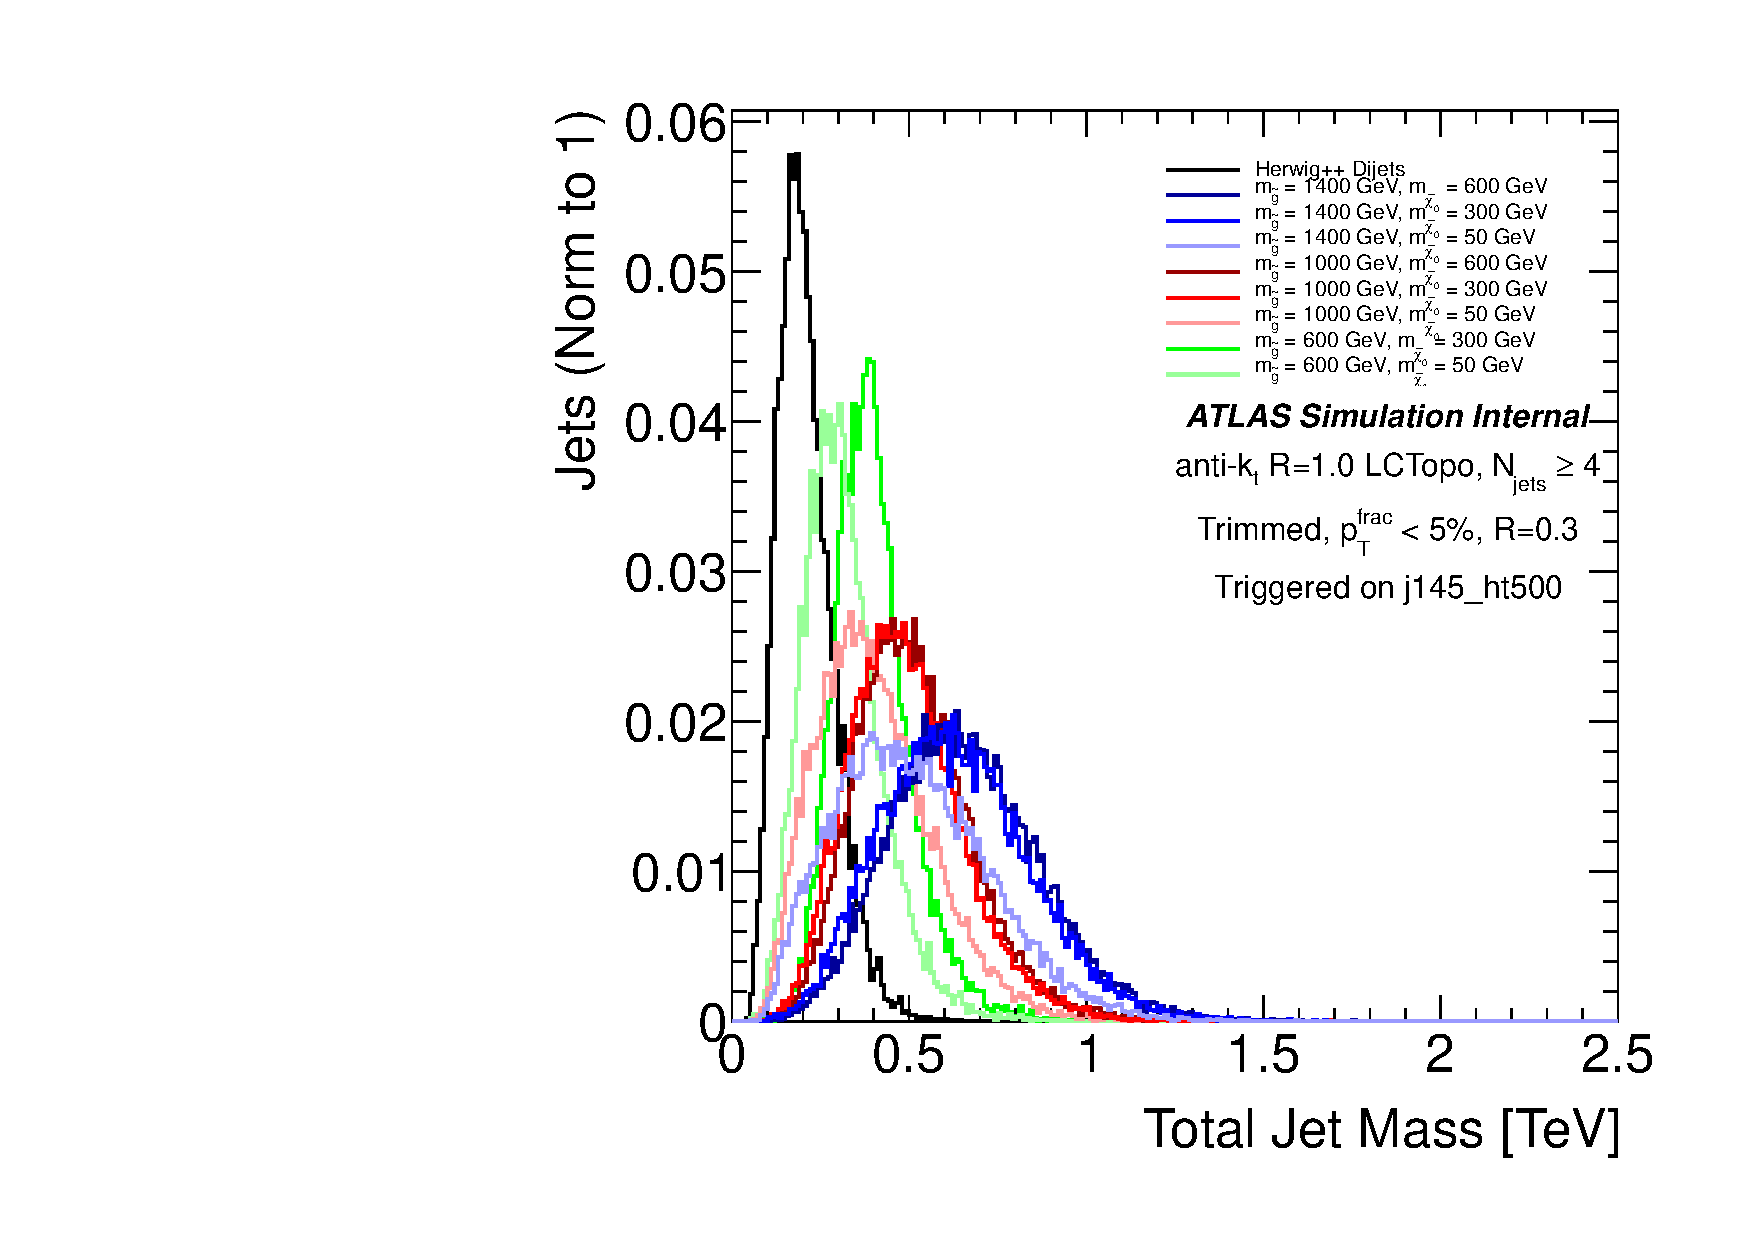
\includegraphics[width=0.45\textwidth]{INT/AntiKt10LCTopoTrimmedPtFrac5SmallR30_j145_ht500_NjetIncl_NFatJetMin4_MJ4_RPVGluino.pdf}}
\subfigure{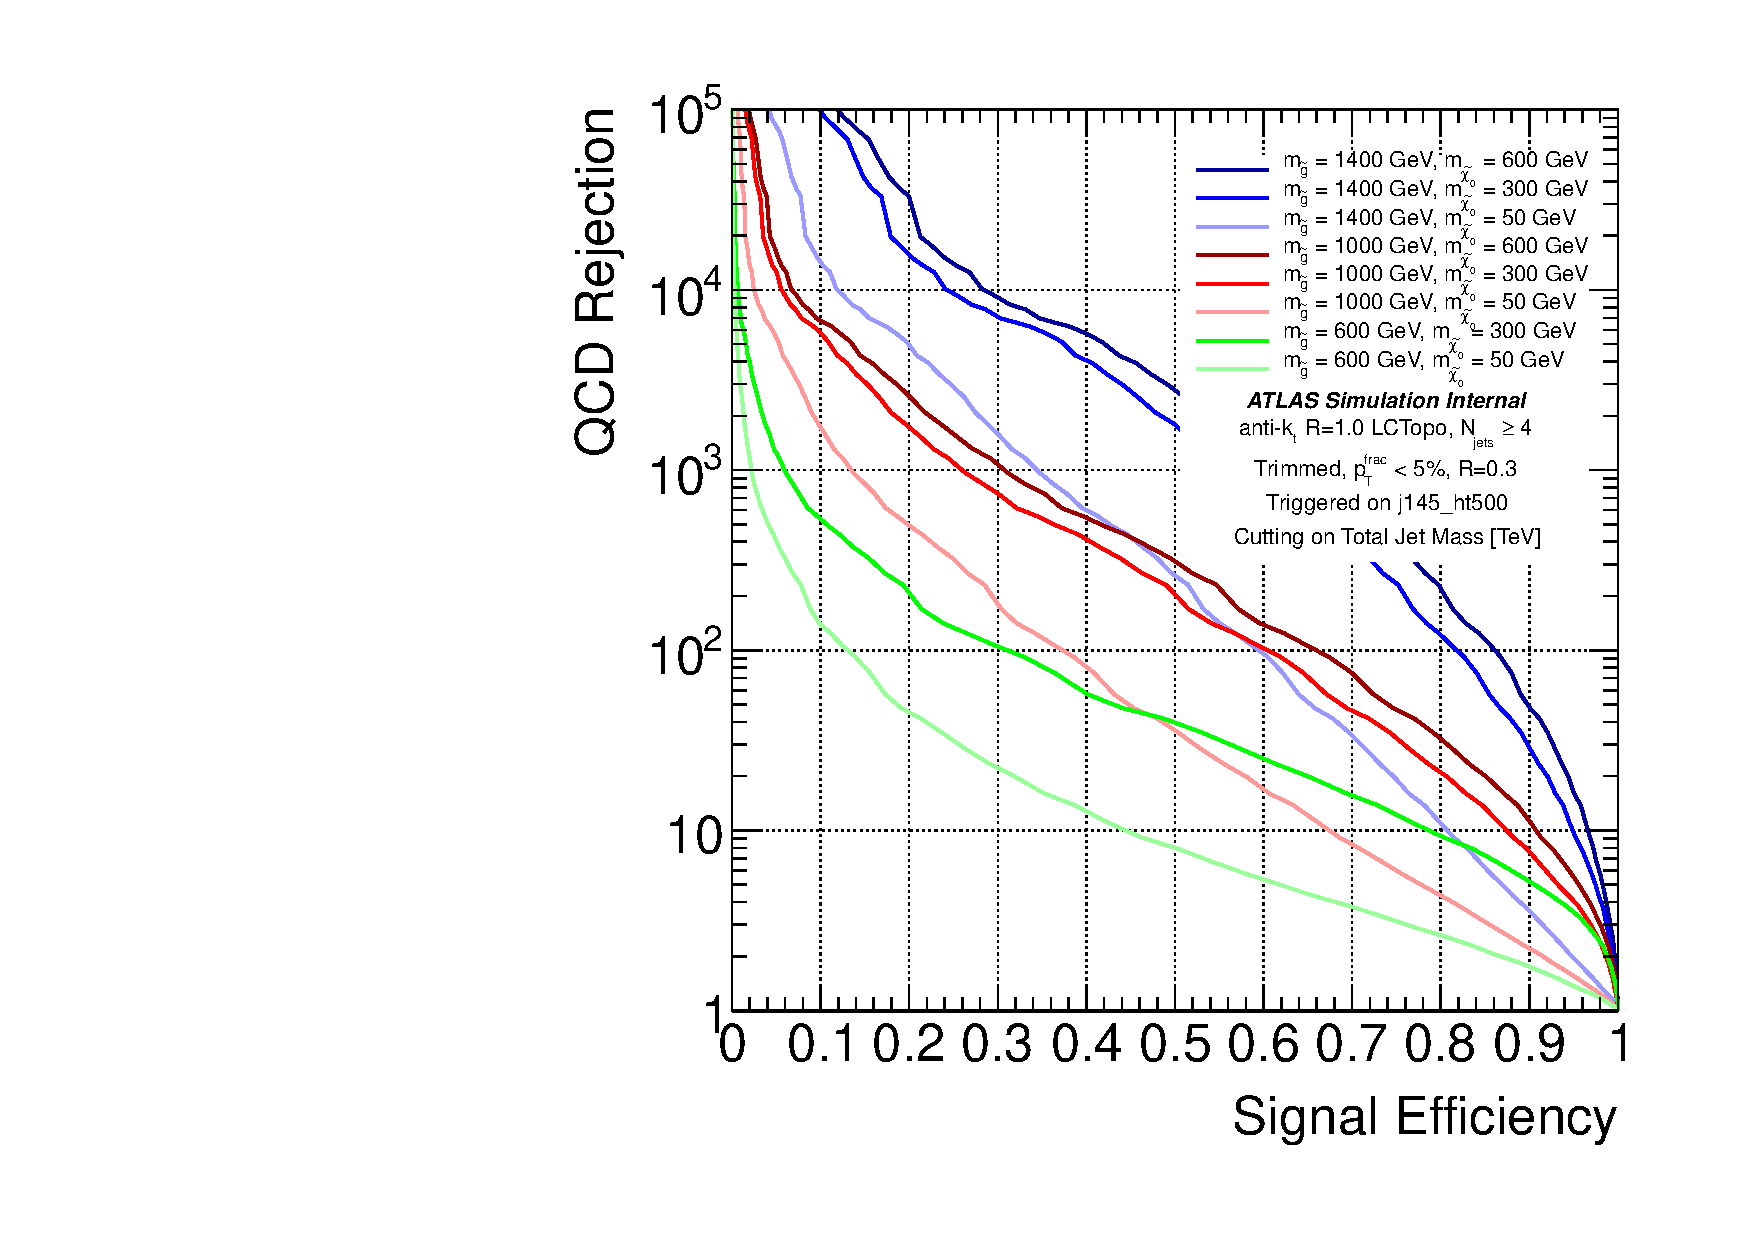
\includegraphics[width=0.45\textwidth]{INT/AntiKt10LCTopoTrimmedPtFrac5SmallR30_j145_ht500_NjetIncl_NFatJetMin4_MJ4_g_RPVGluino}}
\label{fig:search:search:optimization:MJ}
\caption{Distribution of \MJ, a variable describing the total mass in the event. Several signal mass points and the \herwigpp di-jet background are shown. The right-hand plot shows the signal efficiency vs. background rejection of a scan of possible cuts on the \MJ distribution.}
\end{figure}

%%%%%%%%%%%%%%%%%%%%%


%%%%%%%%%%%%%%%%%%%%%

\begin{figure}
\centering
\subfigure{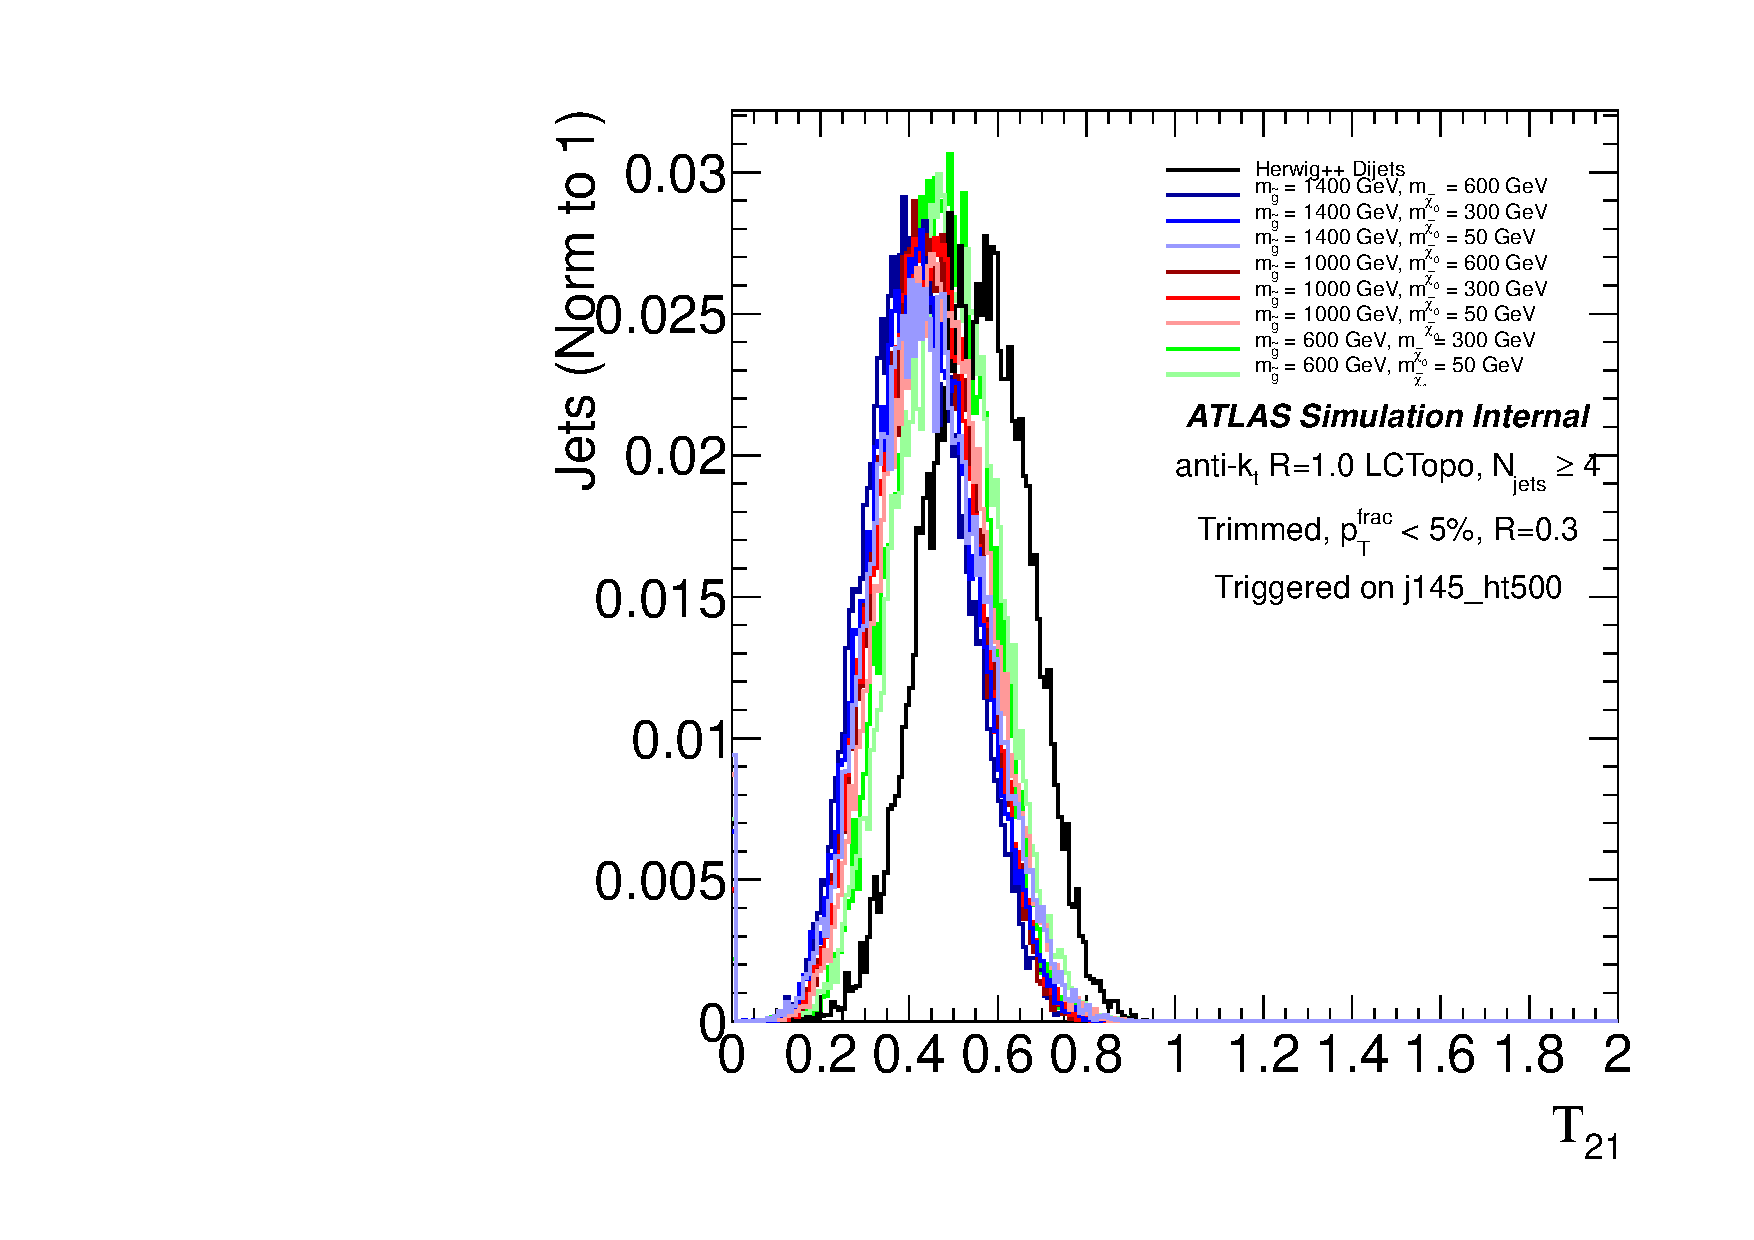
\includegraphics[width=0.45\textwidth]{INT/AntiKt10LCTopoTrimmedPtFrac5SmallR30_j145_ht500_NjetIncl_NFatJetMin4_4T21_RPVGluino.pdf}}
\subfigure{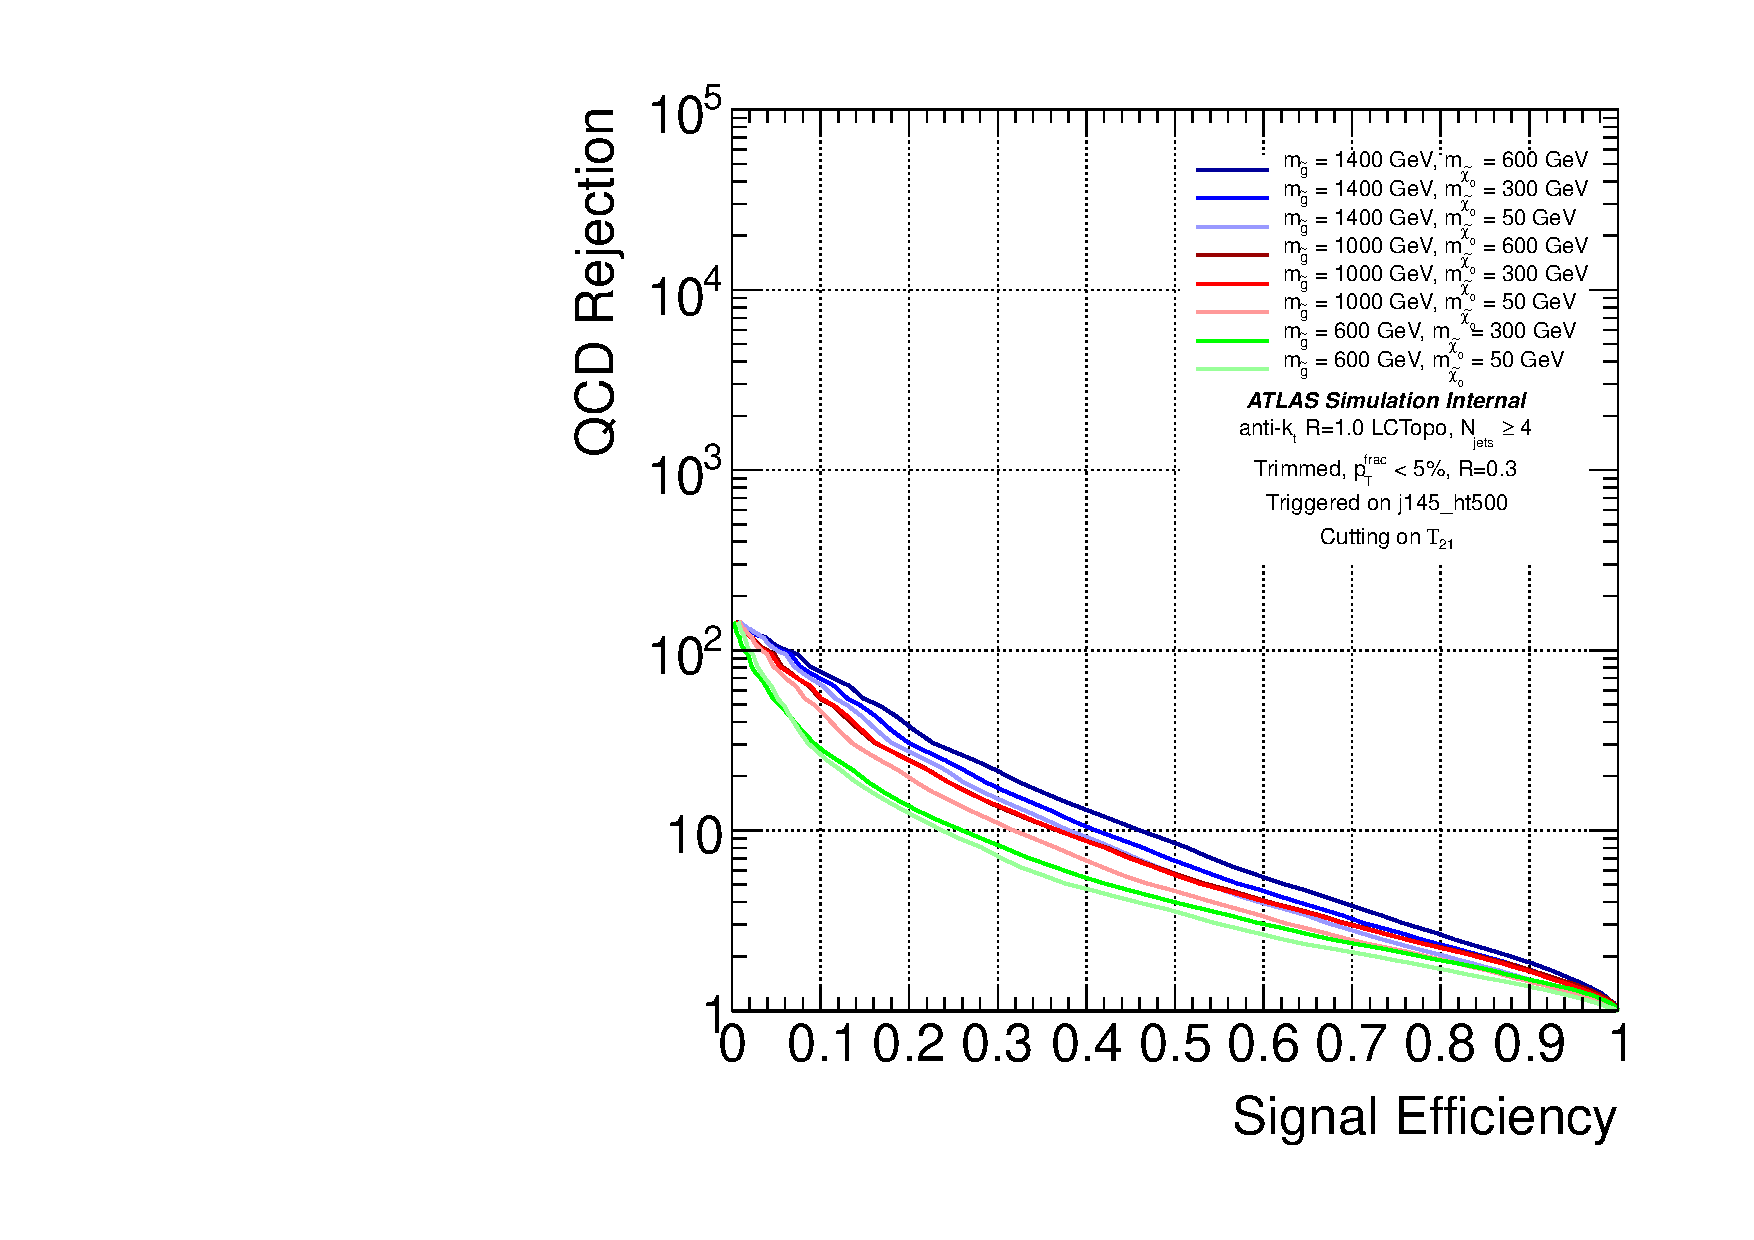
\includegraphics[width=0.45\textwidth]{INT/AntiKt10LCTopoTrimmedPtFrac5SmallR30_j145_ht500_NjetIncl_NFatJetMin4_4T21_g_RPVGluino}}
\label{fig:search:search:optimization:T21}
\caption{Distribution of $T_{21}$, a variable describing the average n-subjettiness ($\tau_{21}$) in the event. Several signal mass points and the \herwigpp di-jet background are shown. The right-hand plot shows the signal efficiency vs. background rejection of a scan of possible cuts on the $T_{21}$ distribution.}
\end{figure}

%%%%%%%%%%%%%%%%%%%%%

%%%%%%%%%%%%%%%%%%%%%

\begin{figure}
\centering
\subfigure{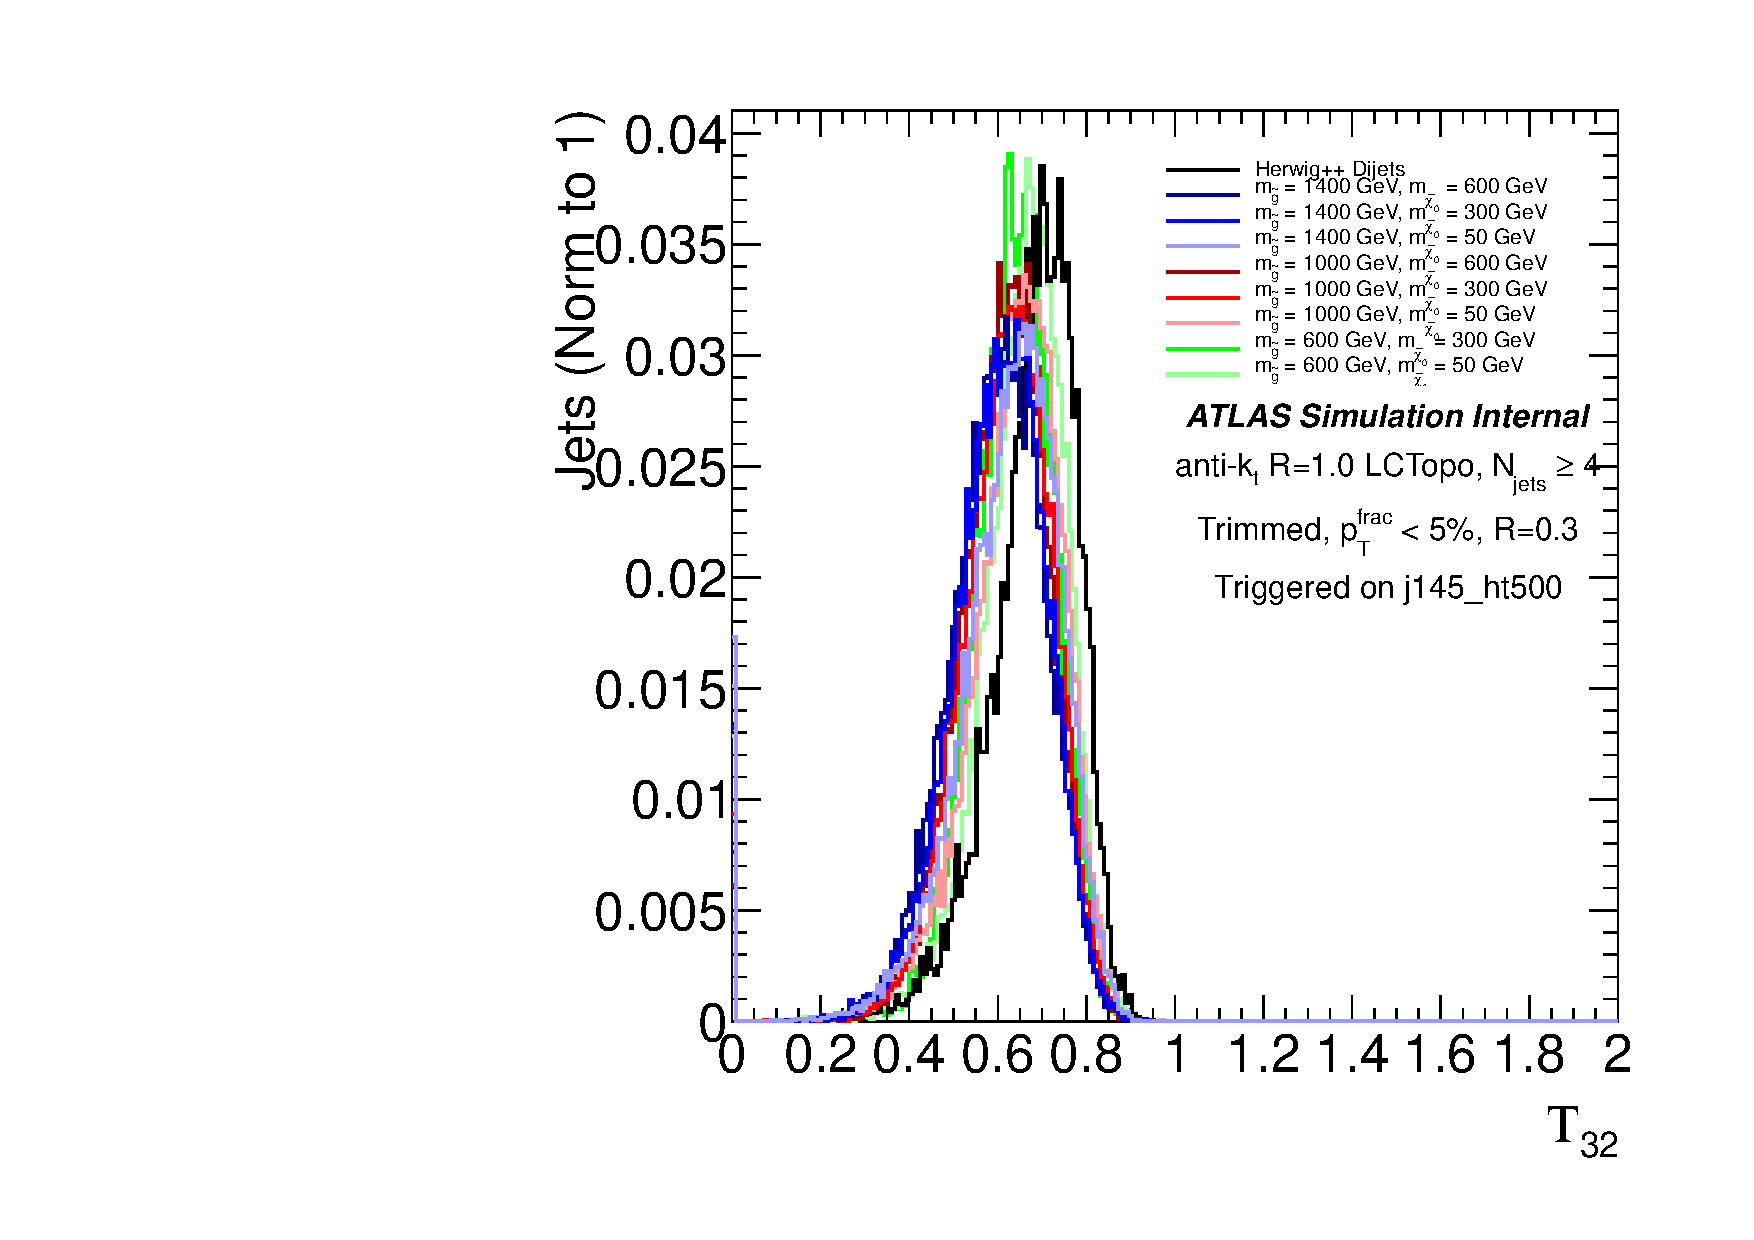
\includegraphics[width=0.45\textwidth]{INT/AntiKt10LCTopoTrimmedPtFrac5SmallR30_j145_ht500_NjetIncl_NFatJetMin4_4T32_RPVGluino.pdf}}
\subfigure{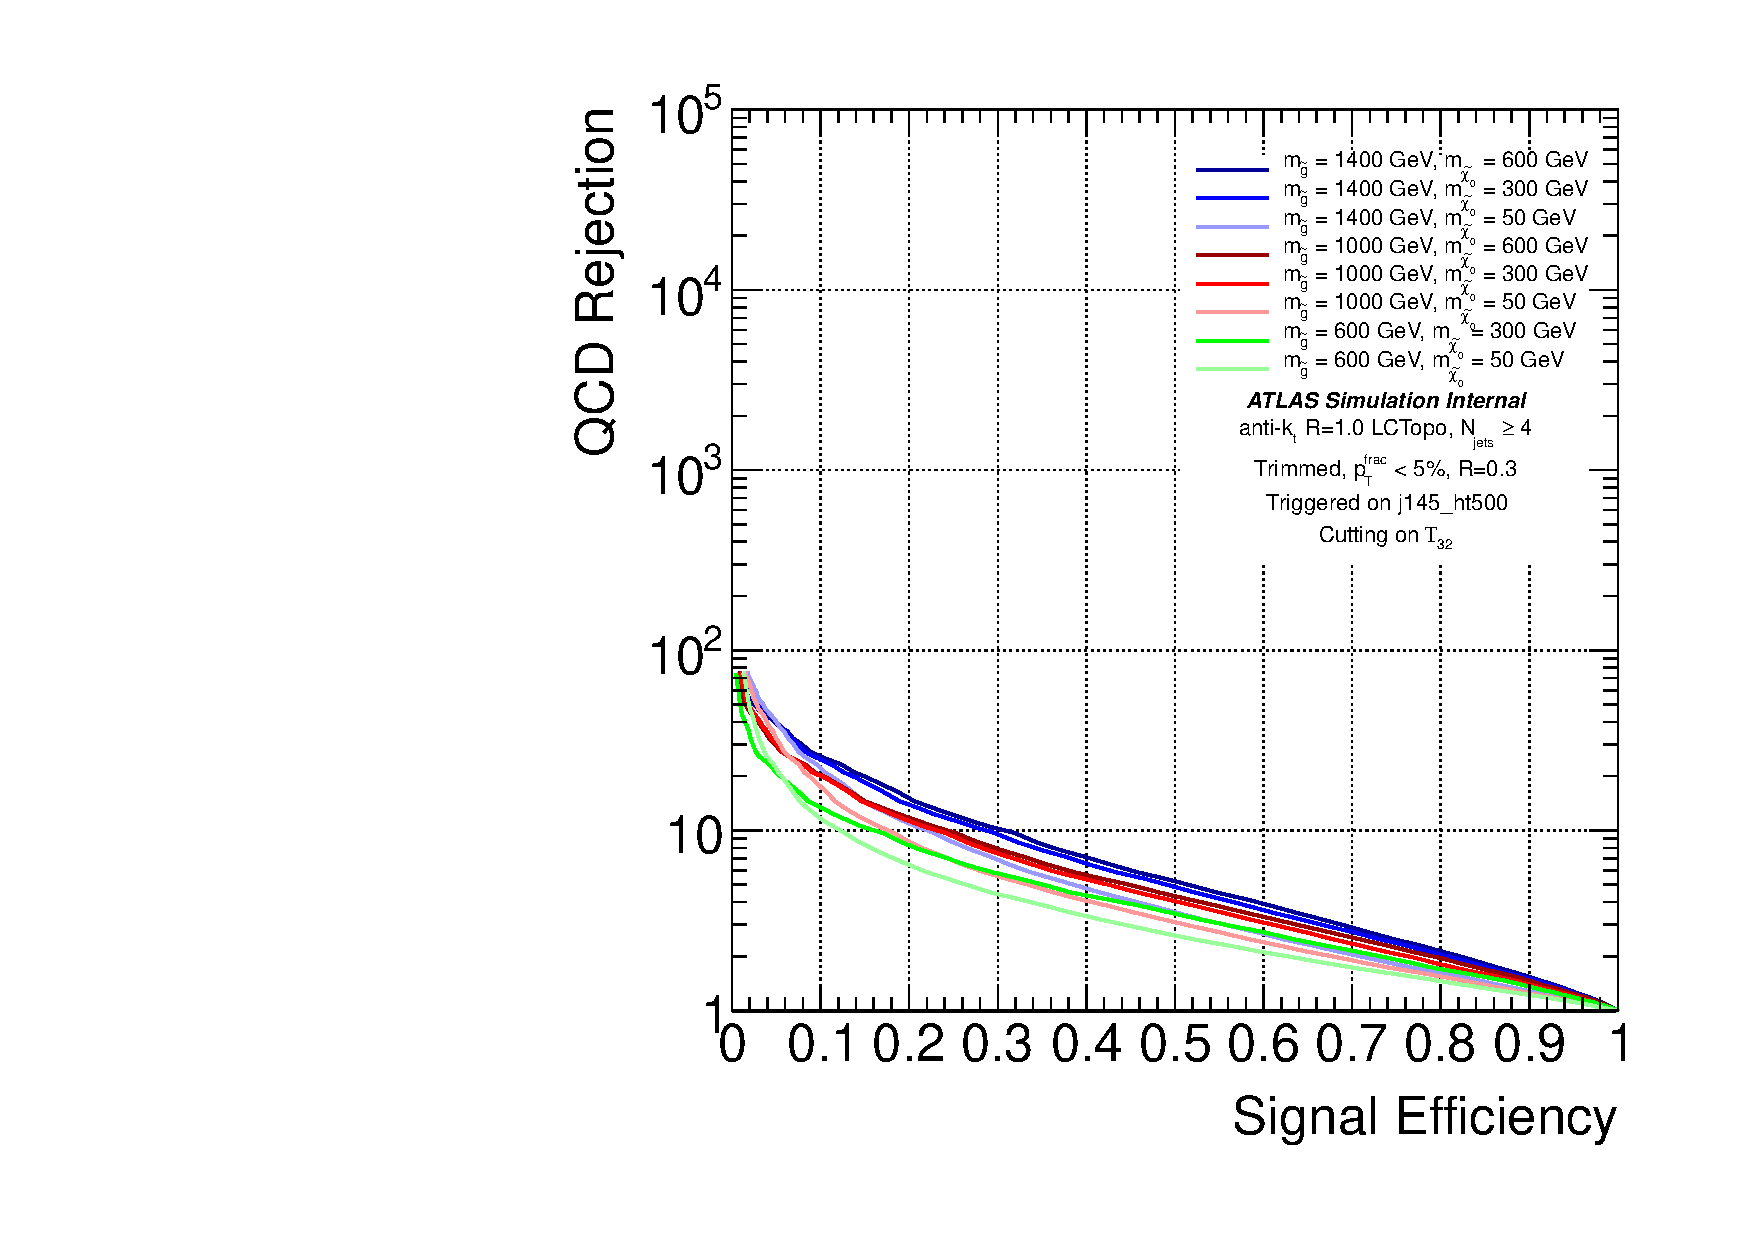
\includegraphics[width=0.45\textwidth]{INT/AntiKt10LCTopoTrimmedPtFrac5SmallR30_j145_ht500_NjetIncl_NFatJetMin4_4T32_g_RPVGluino}}
\label{fig:search:search:optimization:T32}
\caption{Distribution of $T_{32}$, a variable describing the average n-subjettiness ($\tau_{32}$) in the event. Several signal mass points and the \herwigpp di-jet background are shown. The right-hand plot shows the signal efficiency vs. background rejection of a scan of possible cuts on the $T_{32}$ distribution.}
\end{figure}

%%%%%%%%%%%%%%%%%%%%%



%%%%%%%%%%%%%%%%%%%%%

\begin{figure}
\centering
\subfigure{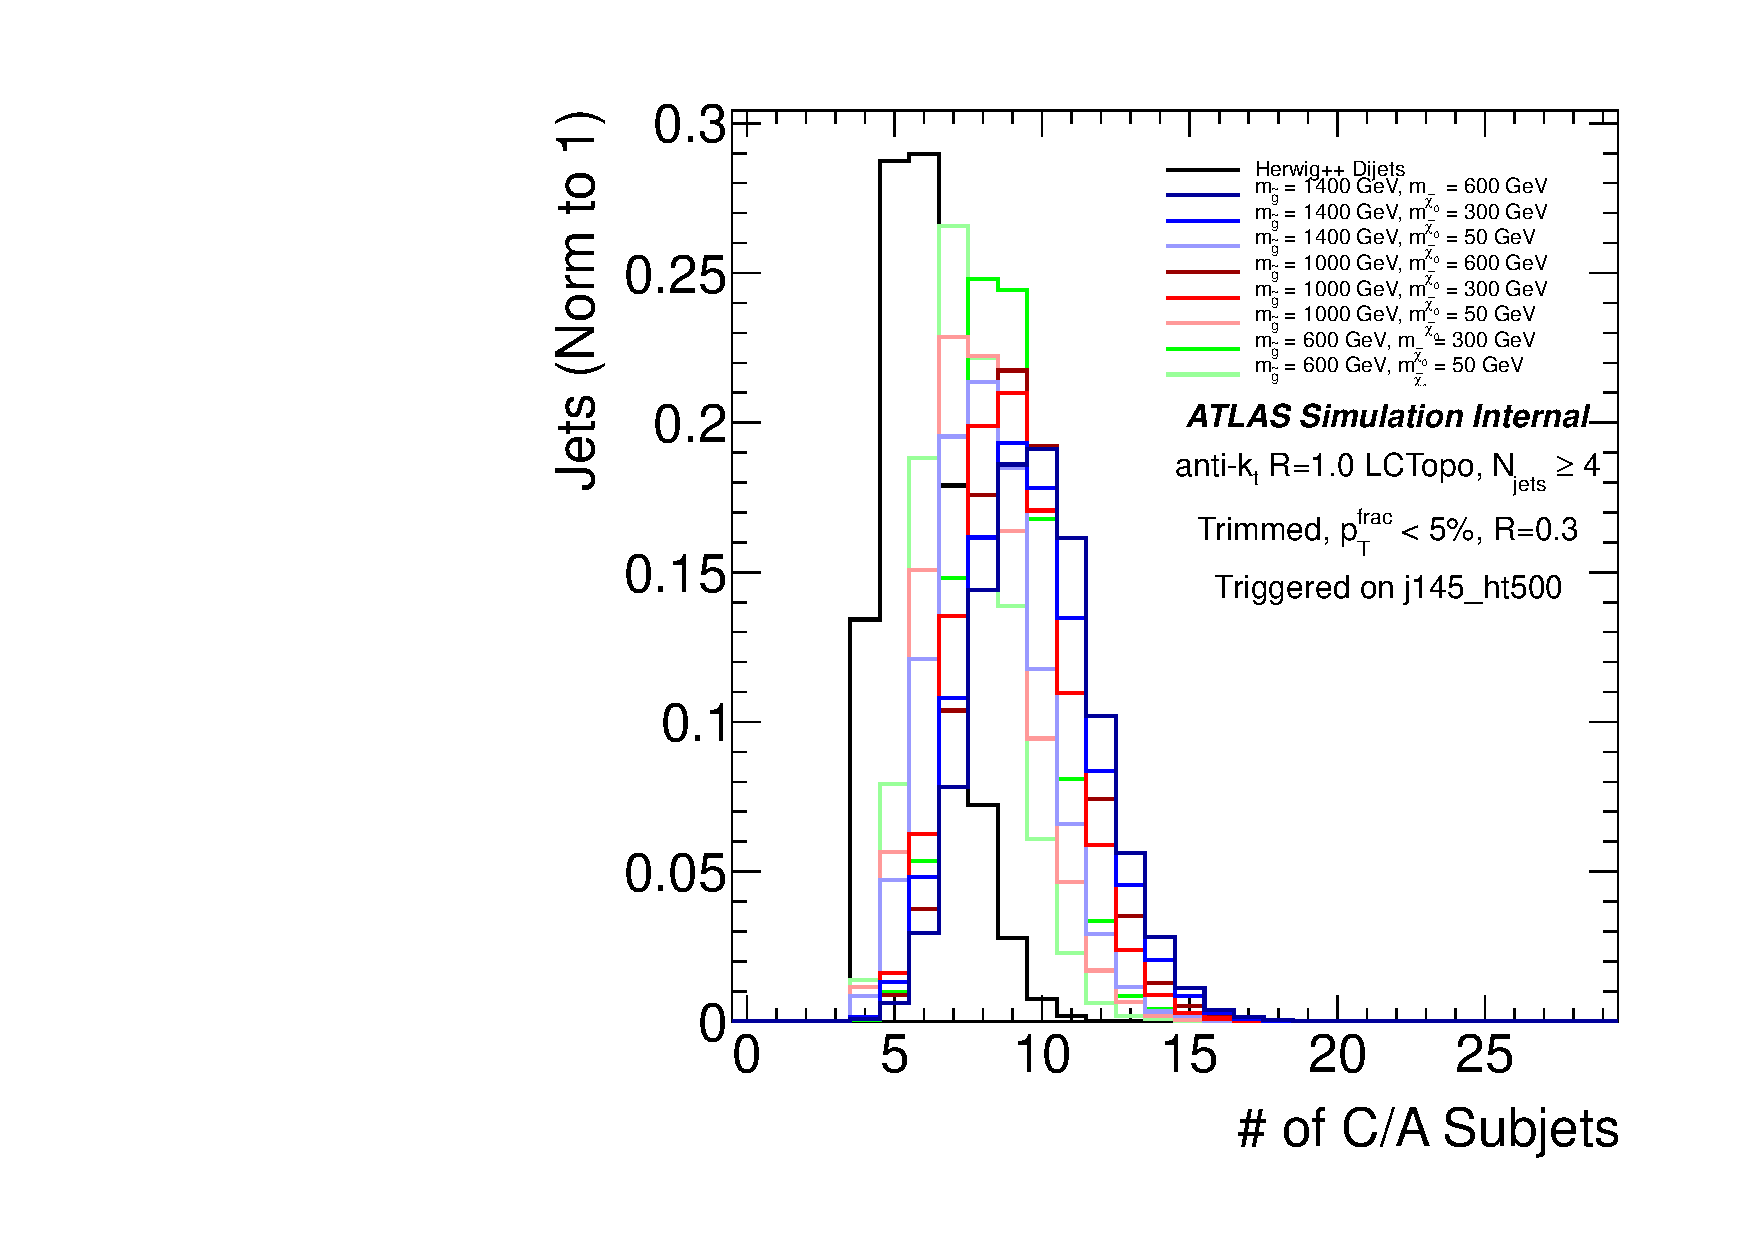
\includegraphics[width=0.45\textwidth]{INT/AntiKt10LCTopoTrimmedPtFrac5SmallR30_j145_ht500_NjetIncl_NFatJetMin4_NCASub4_RPVGluino.pdf}}
\subfigure{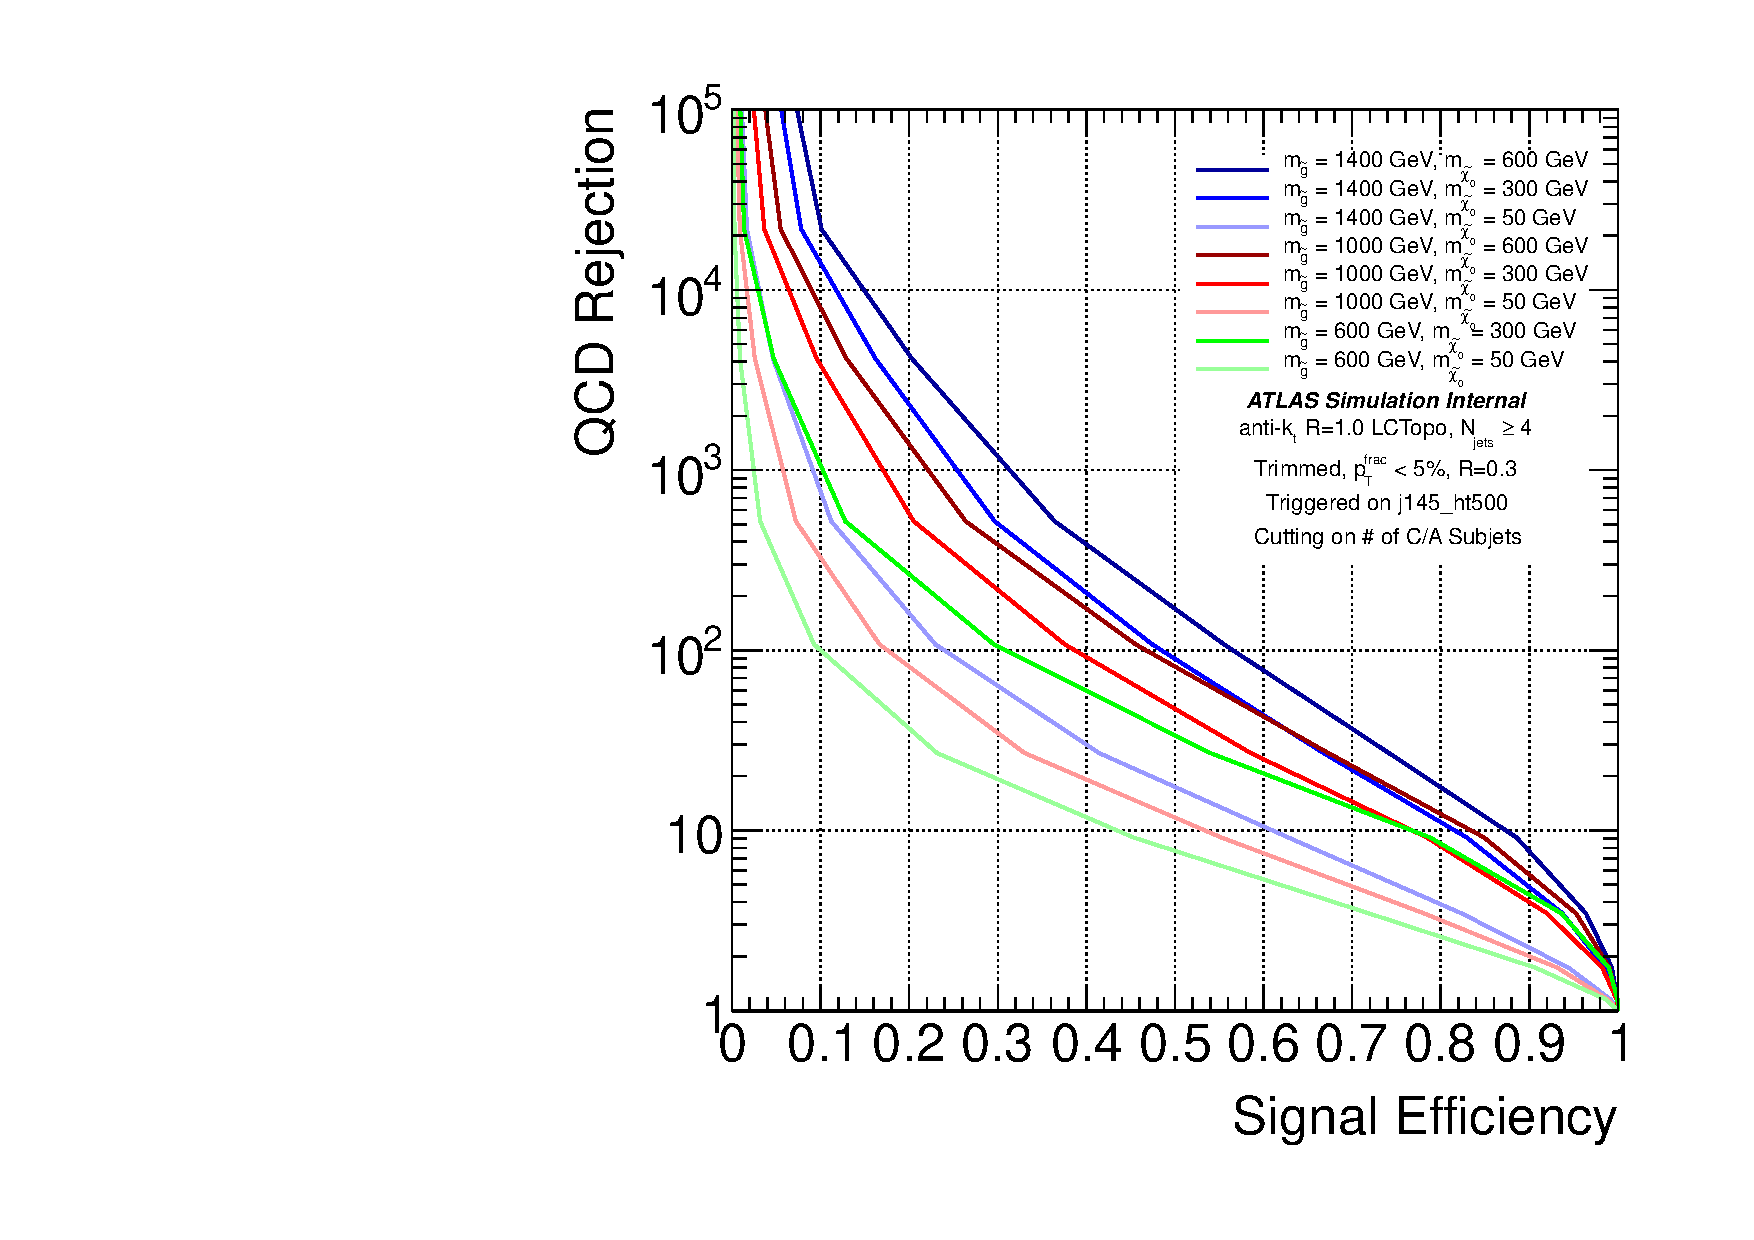
\includegraphics[width=0.45\textwidth]{INT/AntiKt10LCTopoTrimmedPtFrac5SmallR30_j145_ht500_NjetIncl_NFatJetMin4_NCASub4_g_RPVGluino}}
\label{fig:search:search:optimization:NCA}
\caption{Distribution of $N_{CA}$, a variable describing the total number of C/A subjets in the event. Several signal mass points and the \herwigpp di-jet background are shown. The right-hand plot shows the signal efficiency vs. background rejection of a scan of possible cuts on the $N_{CA}$ distribution.}
\end{figure}

%%%%%%%%%%%%%%%%%%%%%



%%%%%%%%%%%%%%%%%%%%%

\begin{figure}
\centering
\subfigure{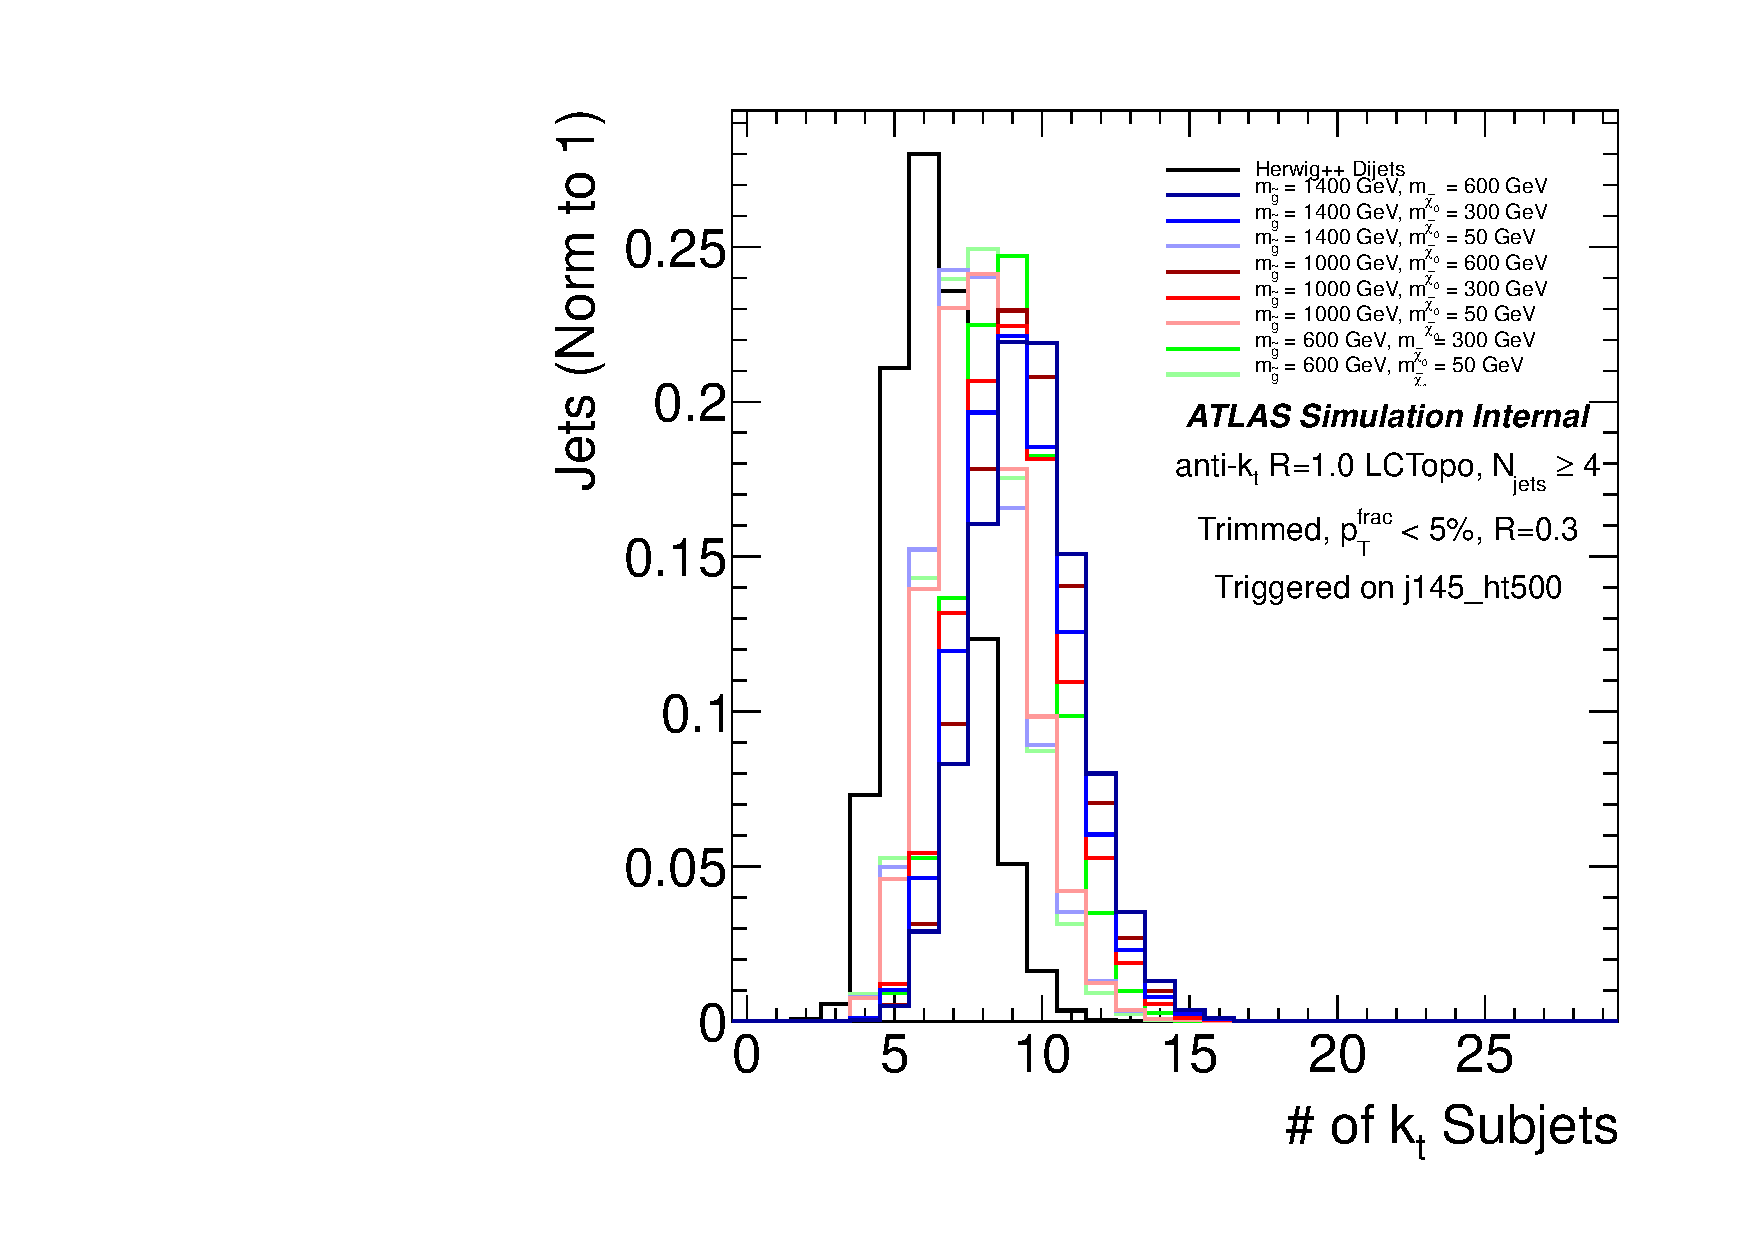
\includegraphics[width=0.45\textwidth]{INT/AntiKt10LCTopoTrimmedPtFrac5SmallR30_j145_ht500_NjetIncl_NFatJetMin4_NKTSub4_RPVGluino.pdf}}
\subfigure{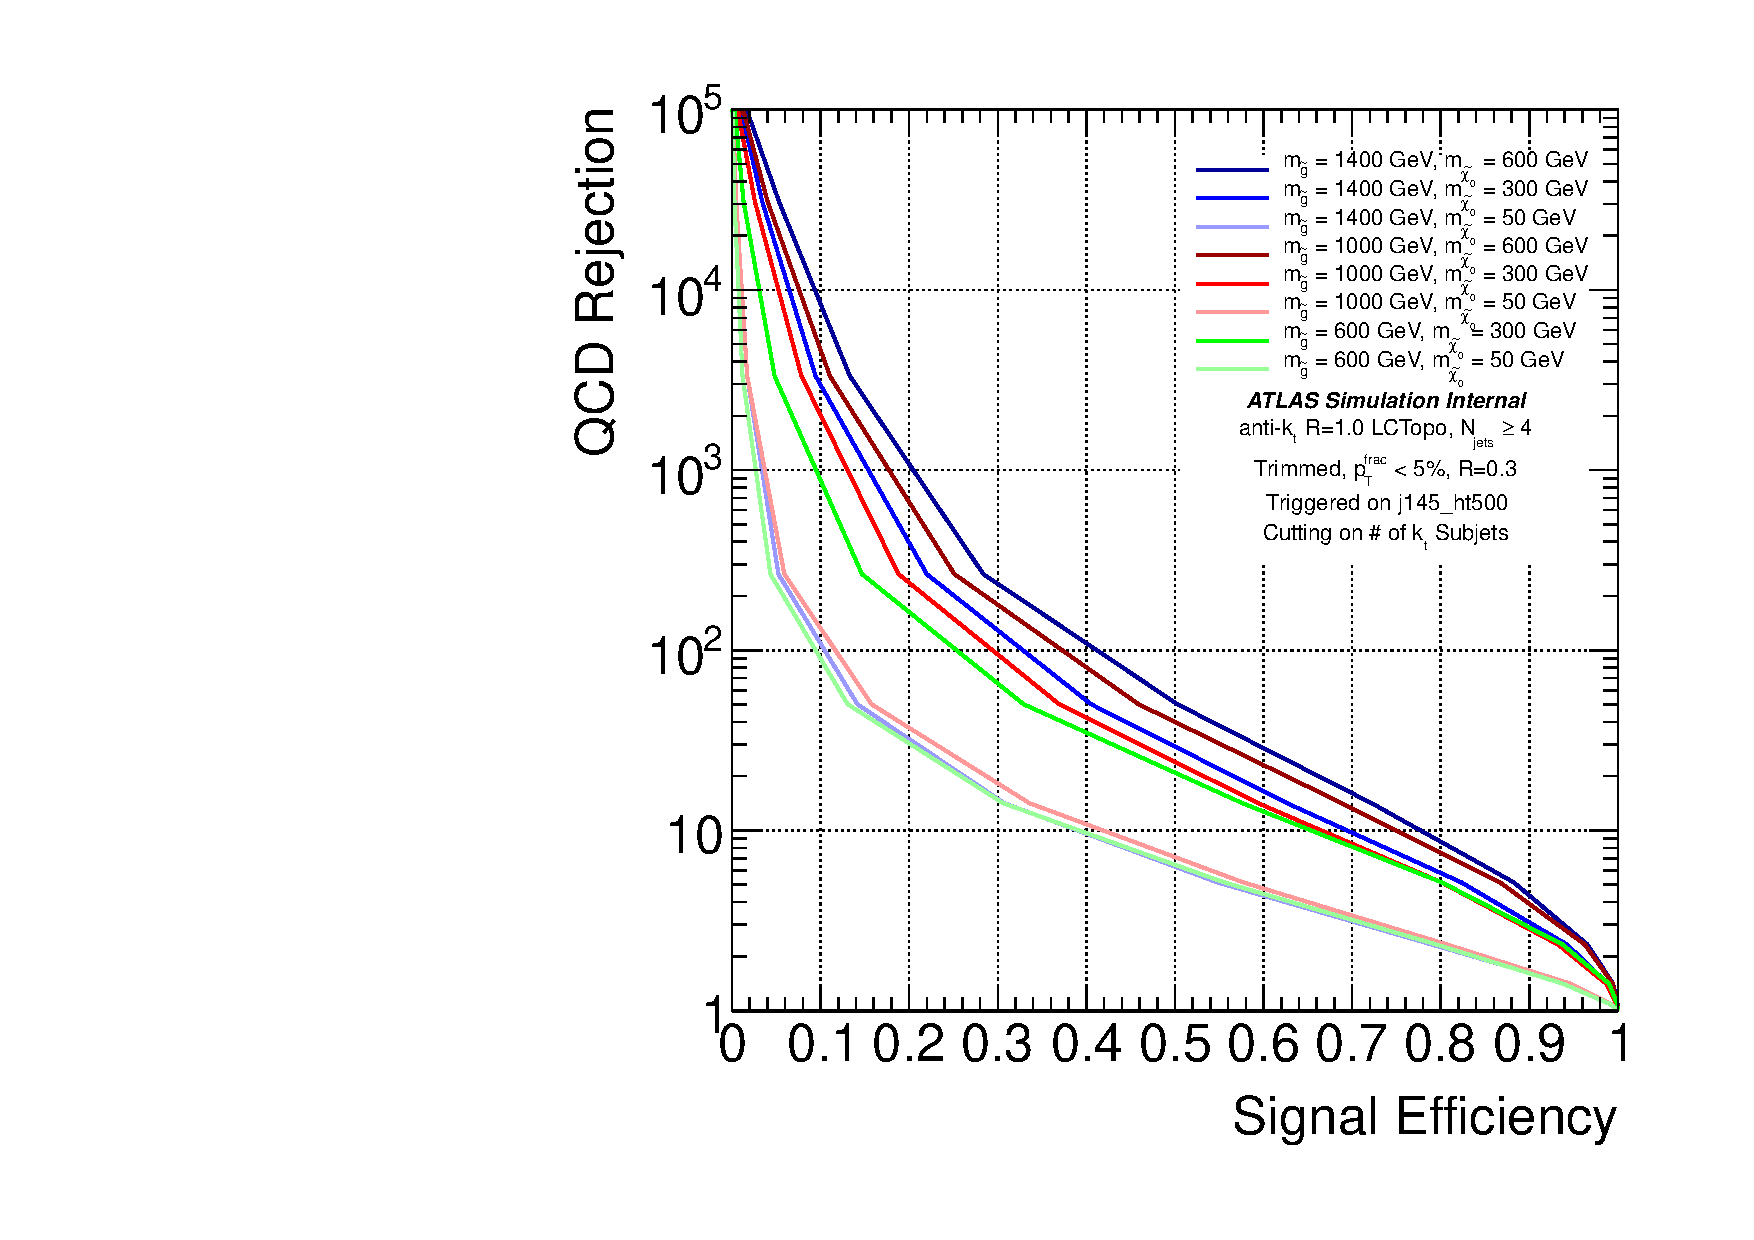
\includegraphics[width=0.45\textwidth]{INT/AntiKt10LCTopoTrimmedPtFrac5SmallR30_j145_ht500_NjetIncl_NFatJetMin4_NKTSub4_g_RPVGluino}}
\label{fig:search:search:optimization:NKT}
\caption{Distribution of $N_{kT}$, a variable describing the total number of \kt subjets in the event. Several signal mass points and the \herwigpp di-jet background are shown. The right-hand plot shows the signal efficiency vs. background rejection of a scan of possible cuts on the $N_{kT}$ distribution.}
\end{figure}

%%%%%%%%%%%%%%%%%%%%%




%%%%%%%%%%%%%%%%%%%%%

\begin{figure}
\centering
\subfigure{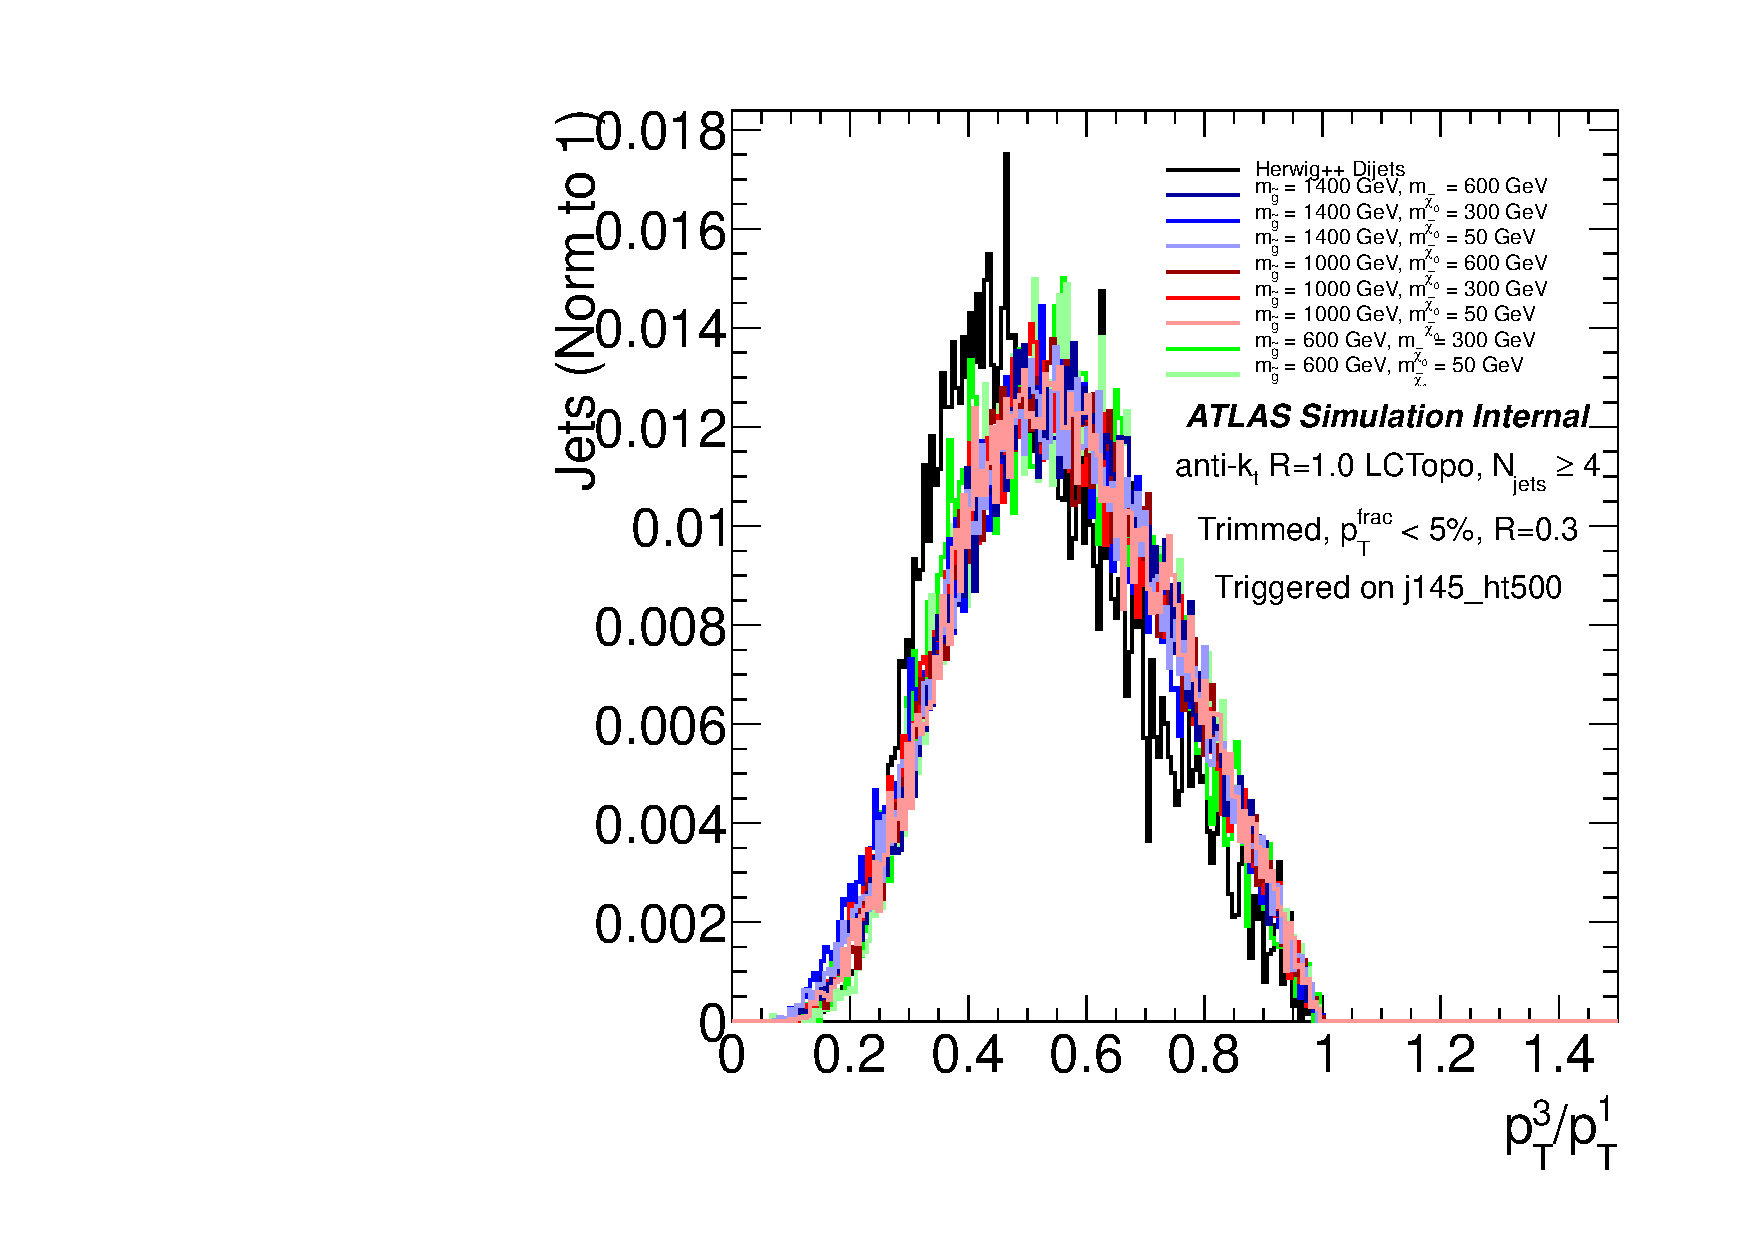
\includegraphics[width=0.45\textwidth]{INT/AntiKt10LCTopoTrimmedPtFrac5SmallR30_j145_ht500_NjetIncl_NFatJetMin4_PT31_RPVGluino.pdf}}
\subfigure{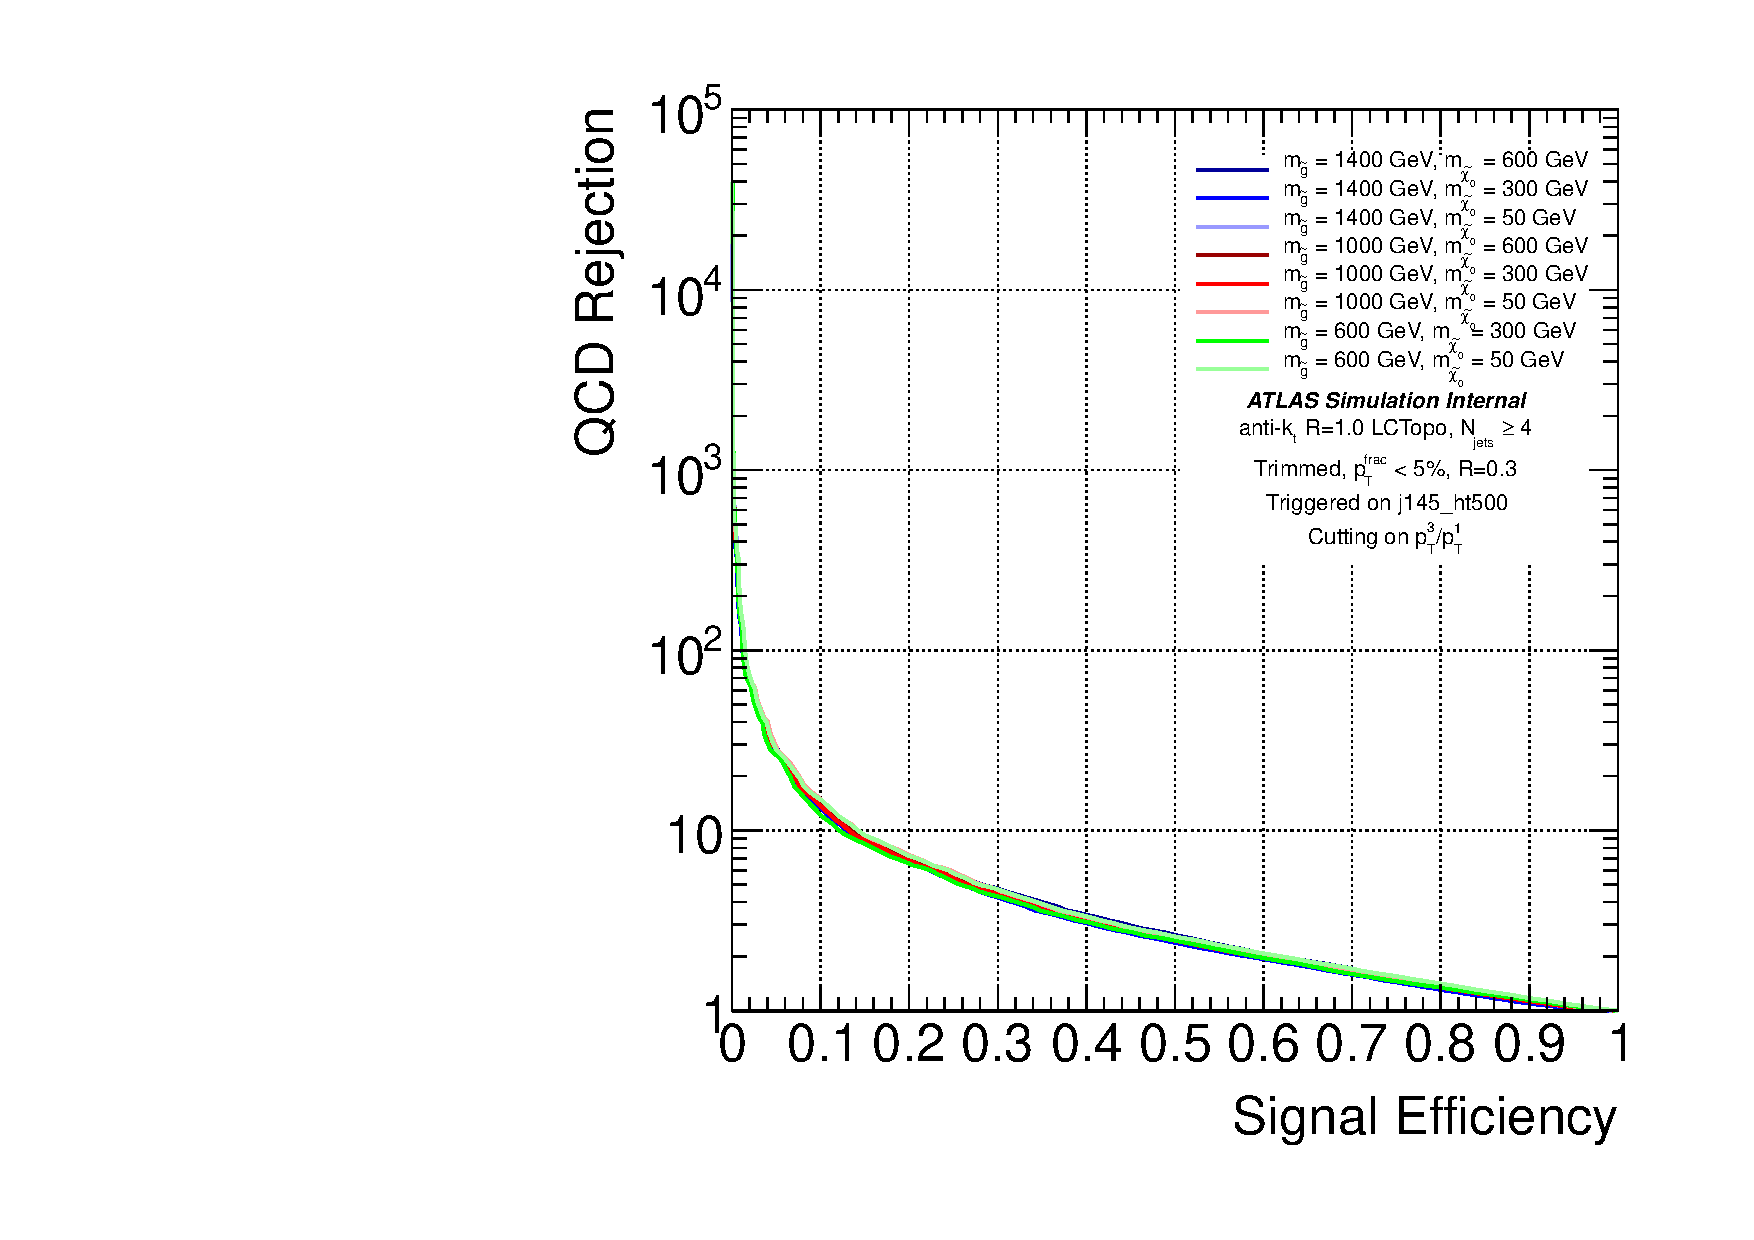
\includegraphics[width=0.45\textwidth]{INT/AntiKt10LCTopoTrimmedPtFrac5SmallR30_j145_ht500_NjetIncl_NFatJetMin4_PT31_g_RPVGluino}}
\label{fig:search:search:optimization:PT31}
\caption{Distribution of $\pt^3/\pt^1$, a variable describing the amount of energy in the third jet in the event. Several signal mass points and the \herwigpp di-jet background are shown. The right-hand plot shows the signal efficiency vs. background rejection of a scan of possible cuts on the $\pt^3/\pt^1$ distribution.}
\end{figure}

%%%%%%%%%%%%%%%%%%%%%


%%%%%%%%%%%%%%%%%%%%%

\begin{figure}
\centering
\subfigure{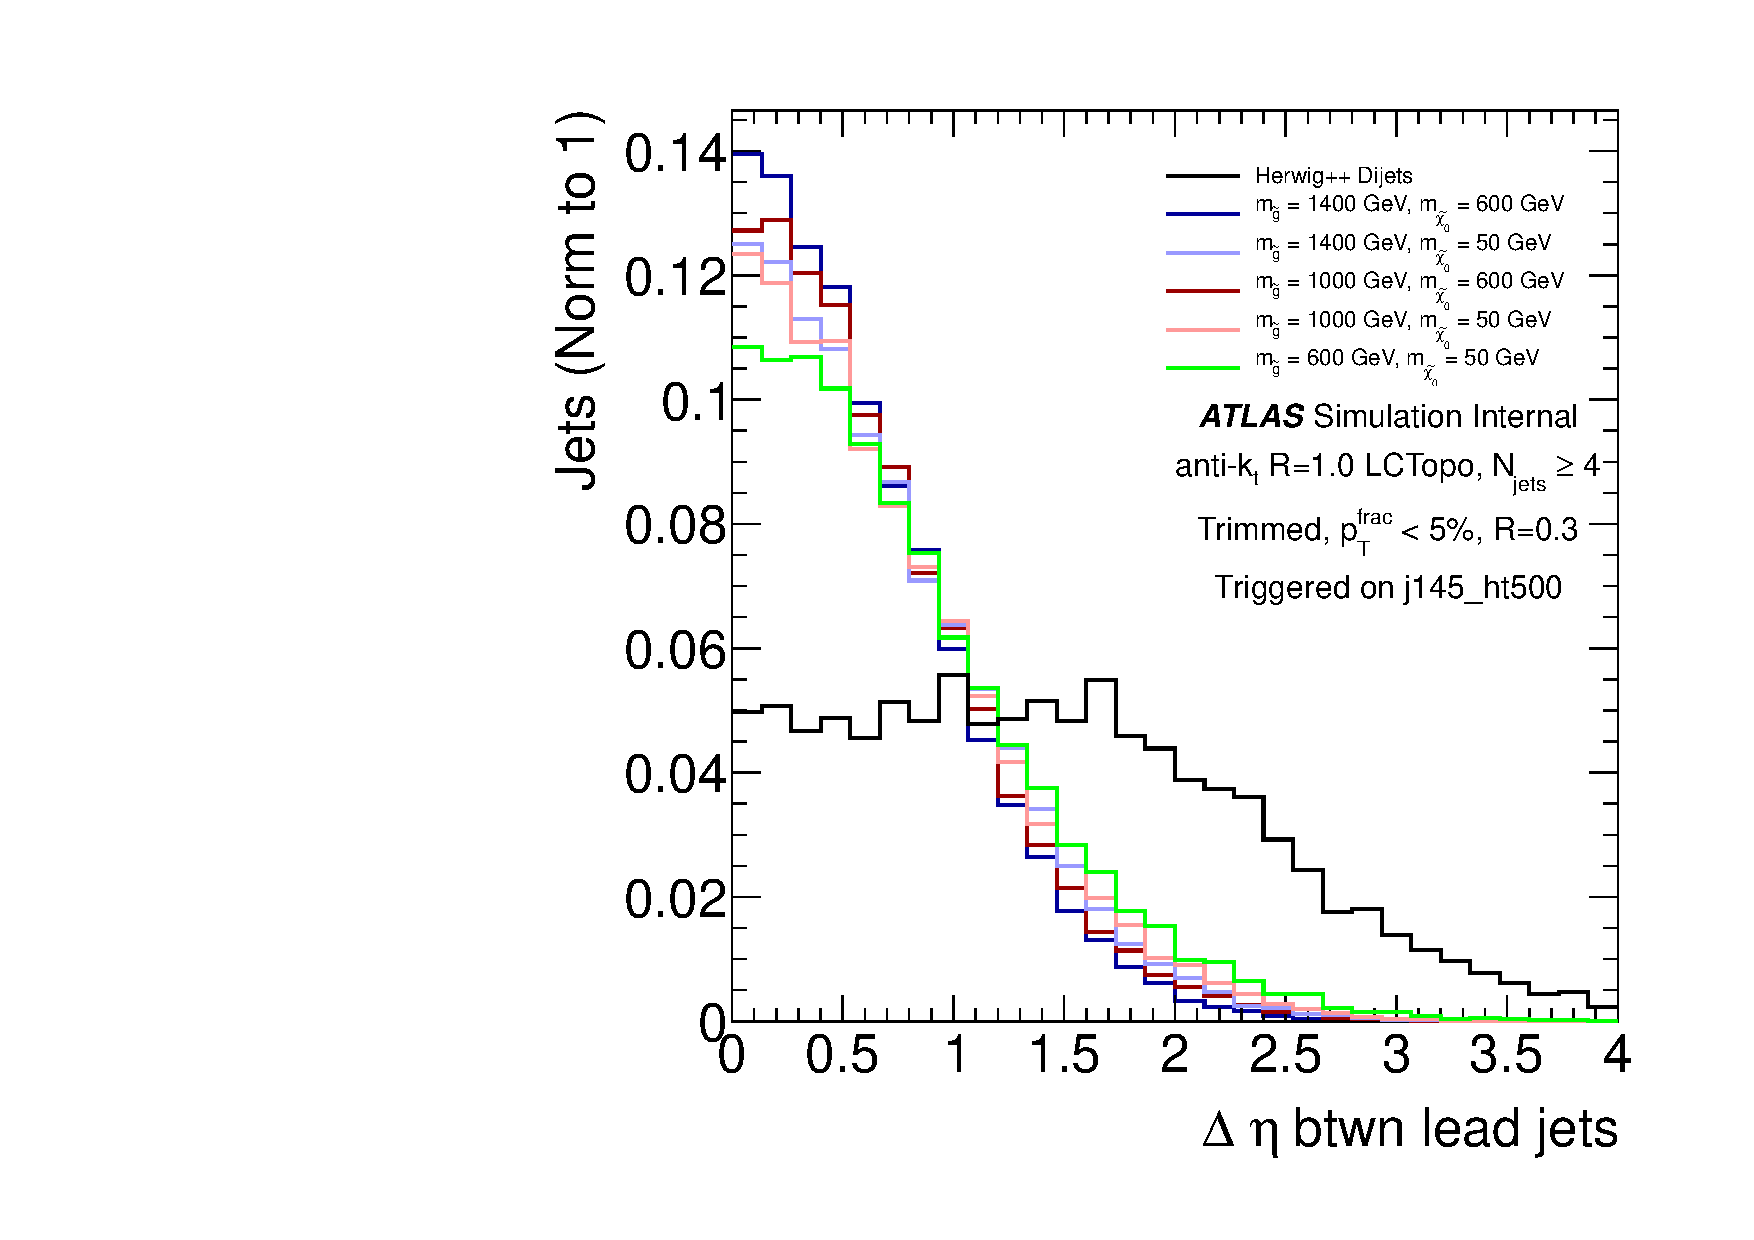
\includegraphics[width=0.45\textwidth]{INT/AntiKt10LCTopoTrimmedPtFrac5SmallR30_j145_ht500_NjetIncl_NFatJetMin4_DEta_RPVGluino.pdf}}
\subfigure{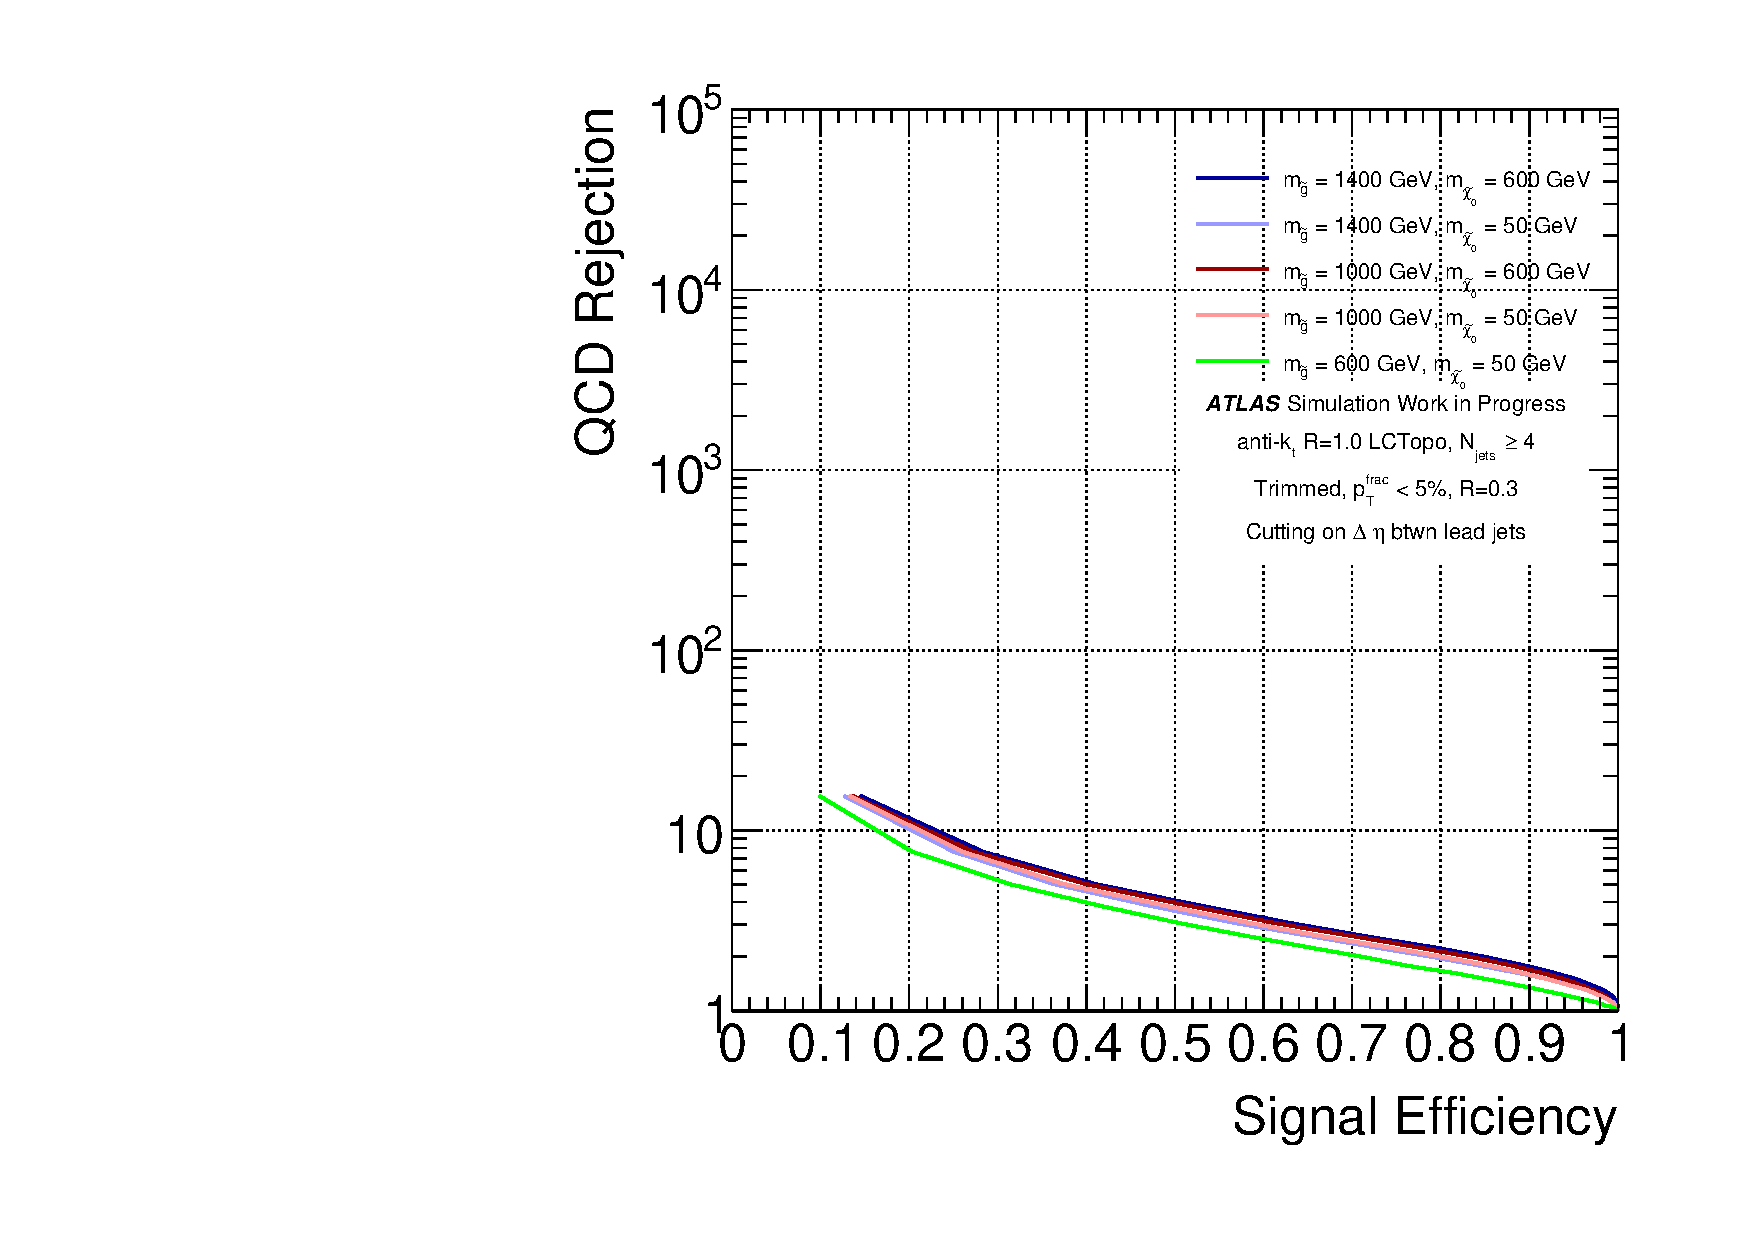
\includegraphics[width=0.45\textwidth]{INT/AntiKt10LCTopoTrimmedPtFrac5SmallR30_j360_a10_NjetIncl_NFatJetMin4_DEta_g_RPVGluino}}
\label{fig:search:search:optimization:DEta}
\caption{Distribution of $\Delta \eta$ a variable describing the difference in pseudo-rapidity between the leading two jets. Several signal mass points and the \herwigpp di-jet background are shown. The right-hand plot shows the signal efficiency vs. background rejection of a scan of possible cuts on the $\Delta \eta$ distribution.}
\end{figure}

%%%%%%%%%%%%%%%%%%%%%

Finally, Figure~\ref{fig:search:search:optimization:All} shows two efficiency vs. rejection curves for two different mass points, comparing all of the various variables previously shown (though $\Delta \eta$ is not shown, its performance is slightly stronger than $\pt^3/\pt^1$ on these plots). Several important conclusions are clear:

\begin{enumerate}
\item While \Ht is sometimes strongest at very high signal efficiency, and $N_{kT}$ and $N_{CA}$ sometimes strongest at very, very low signal efficiency, \MJ is generally the strongest variable by far.
\item \Ht is generally the second strongest variable, though it is a kinematic variable and so the background estimation may not work well with it.
\item $N_{kT}$ and $N_{CA}$ generally work very well-- but integer type variables may be problematic with a Gaussian kernel smoothing.
\item $T_{32}$ and $T_{21}$ perform worse than the subjet counting variables, but do have some power.
\item $\pt^3/\pt^1$ has comparatively low power.
\end{enumerate}

%%%%%%%%%%%%%%%%%%%%%

\begin{figure}
\centering
\subfigure{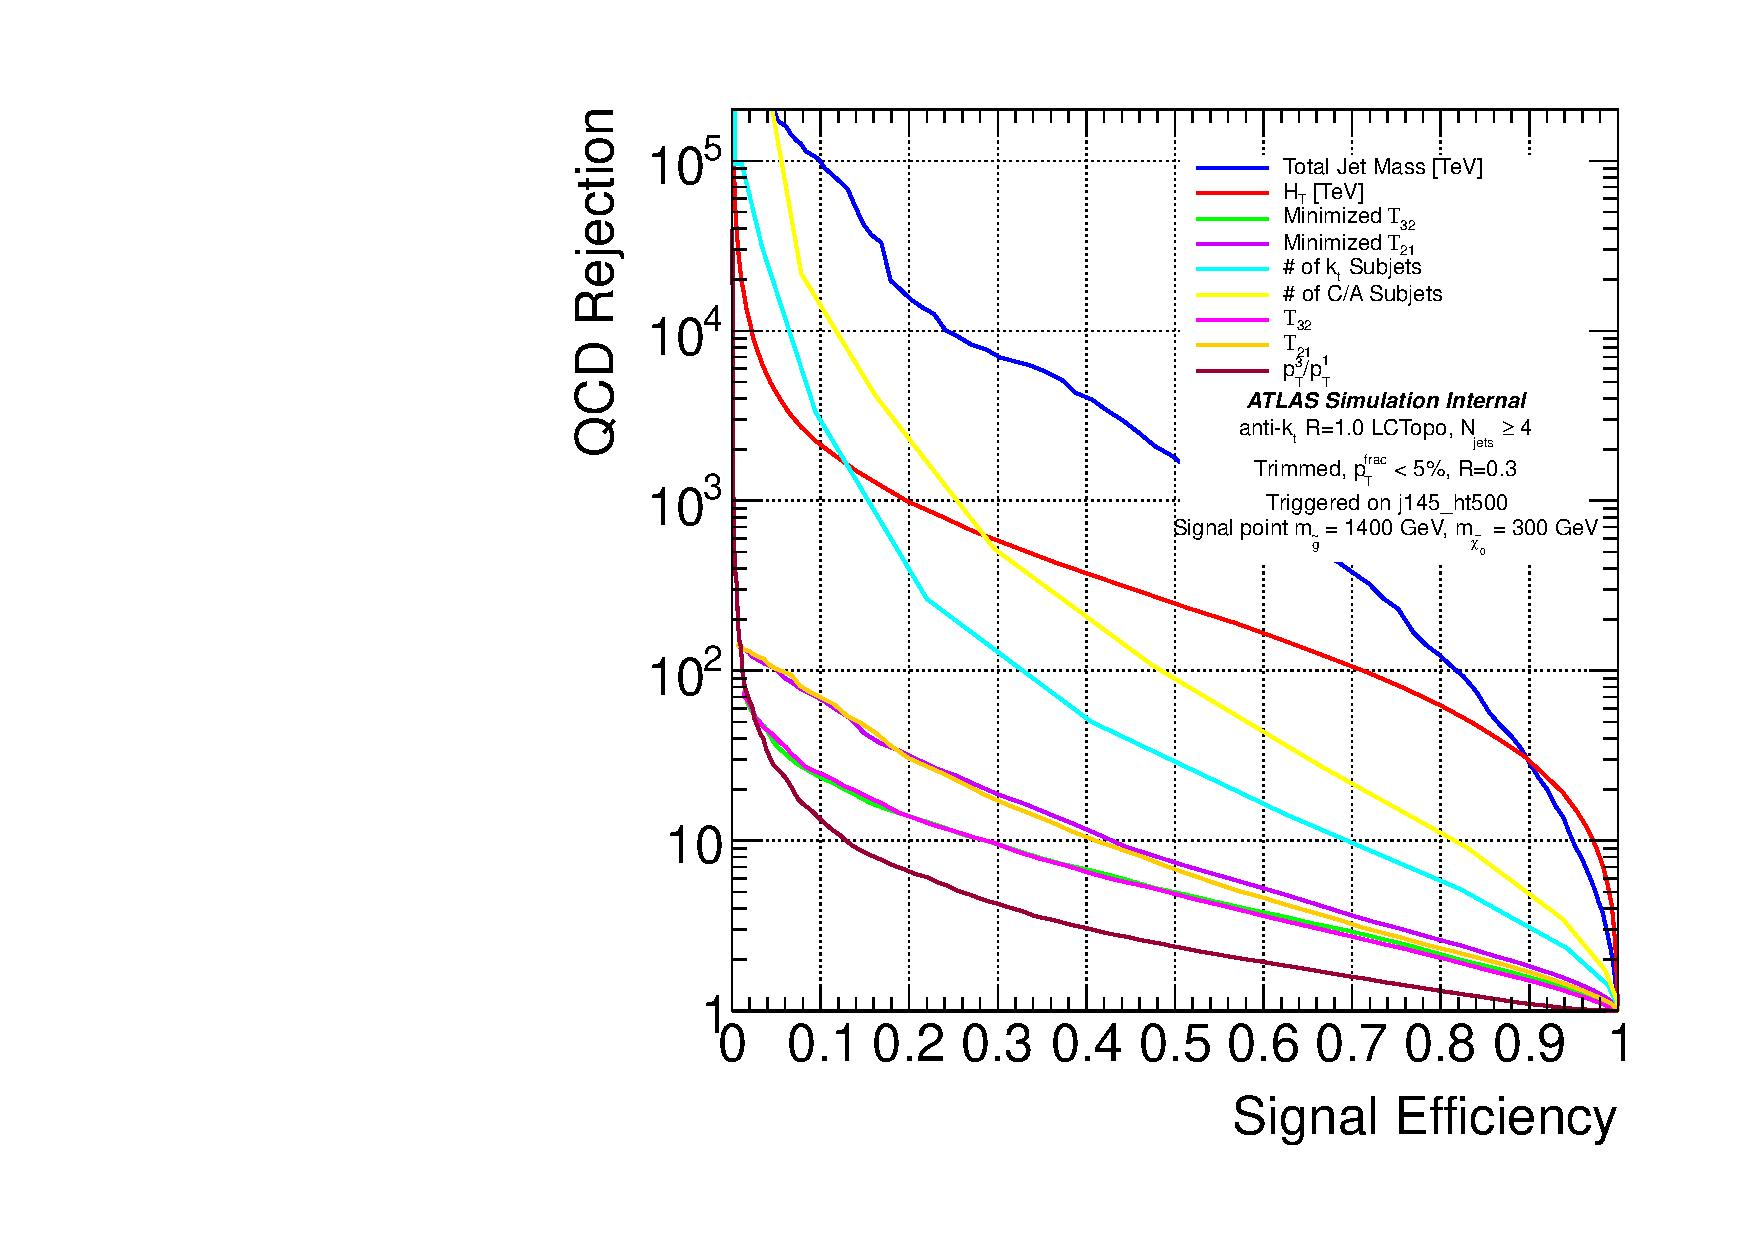
\includegraphics[width=0.45\textwidth]{INT/AntiKt10LCTopoTrimmedPtFrac5SmallR30_j145_ht500_NjetIncl_NFatJetMin4_SigPoint2_g_RPVGluino}}
\subfigure{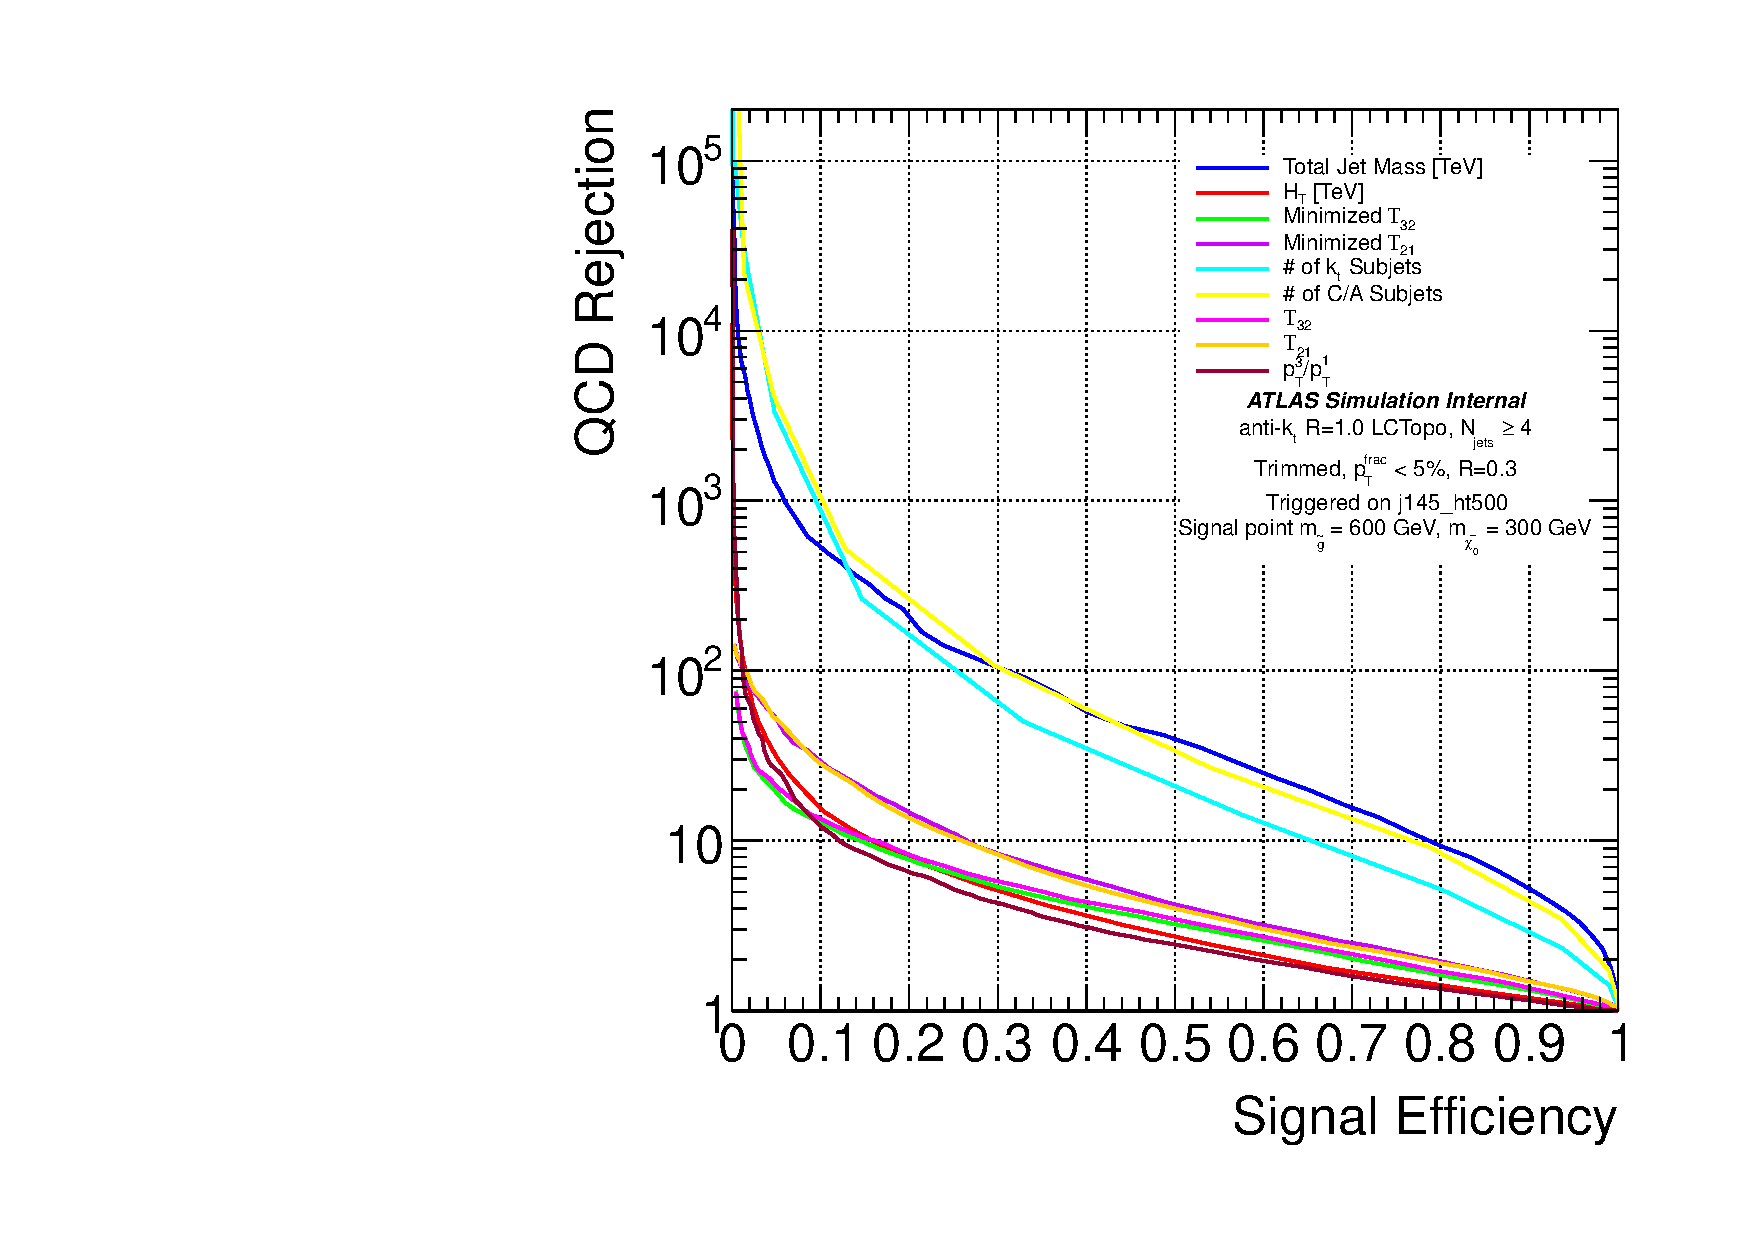
\includegraphics[width=0.45\textwidth]{INT/AntiKt10LCTopoTrimmedPtFrac5SmallR30_j145_ht500_NjetIncl_NFatJetMin4_SigPoint7_g_RPVGluino}}
\label{fig:search:search:optimization:All}
\caption{Signal efficiency vs. background rejection curves for two pass points, comparing the power of various variables. $\Delta \eta$ is not shown, but has similar power (though slightly stronger) than $\pt^3 / \pt^1$.}
\end{figure}

%%%%%%%%%%%%%%%%%%%%%

From this set of results, it is clear that \MJ is a good candidate for a final discriminant variable which can apply the most discrimination between signal and background. There are several other candidates for the second variable used for defining signal and control regions, but these need two-dimensional correlation studies in order to understand the best pairing.

Throughout these studies, the event-level variables have been constructed from the leading 4 jets (recall that the signal region was pre-selected to have $>=4$ jets. Other possibilities-- such as constructing the substructure observable from only the leading 2 jets-- could potentially make the background estimation easier, but come at a price of slightly reduced discrimination (as the third and fourth jets do have useful substructure information to contribute). Similarly, one could add more jets to the sums/means if they existed, but this was found to not contribute at all to discrimation, and as it would further complicate the background estimation, this strategy was not adopted. For this reasons, all the variables considered simply use the leading 4 jets in the event.

One important consideration, for the sake of the background estimation, is understanding whether the \pt spectrum is sensitive to new physics (as we use the \pt spectrum to determine the background expectation). Figure~\ref{fig:search:search:optimization:pt} shows that the \pt spectrum is essentially unchanged, showing that we can use the kinematics without worry of biasing the background estimate.

%%%%%%%%%%%%%%%%

\begin{figure}
\centering
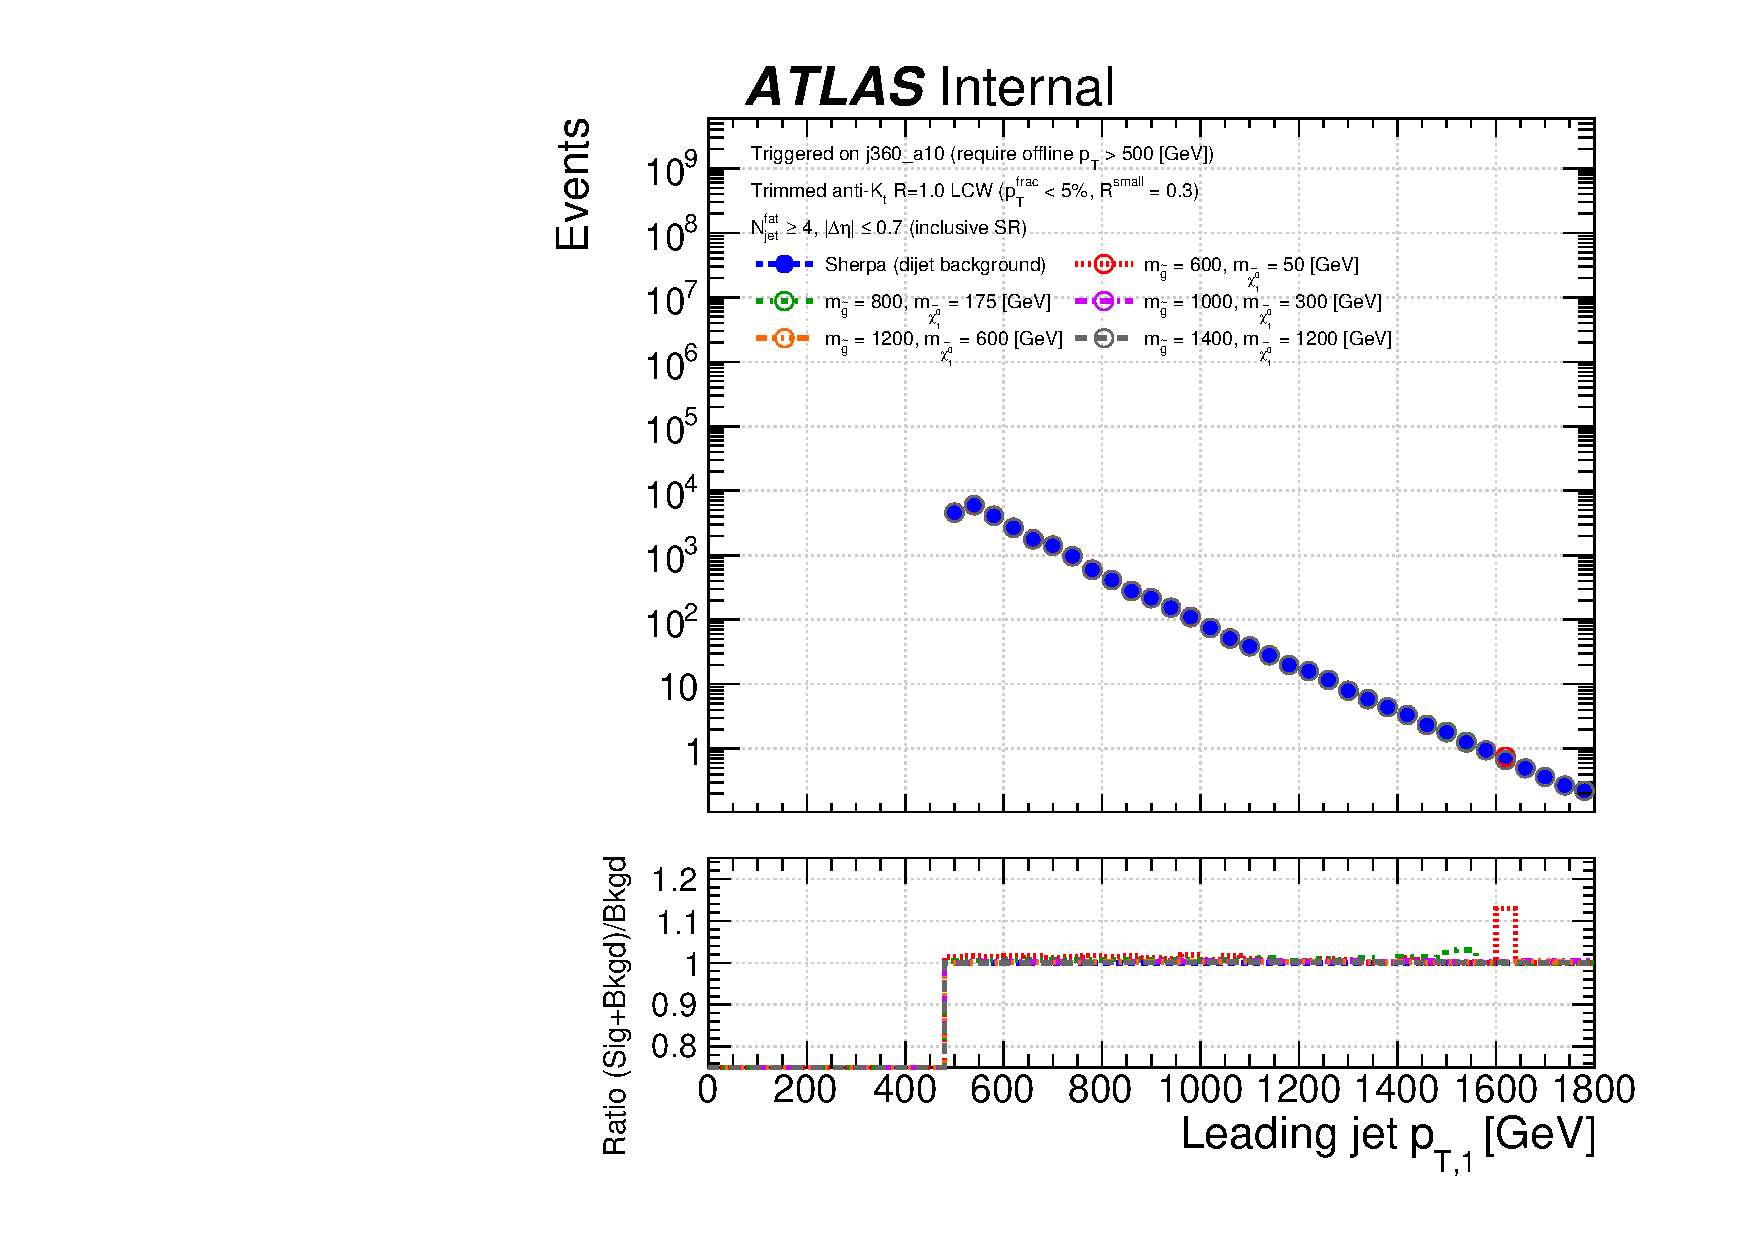
\includegraphics[width=0.5\textwidth]{INT/overlay_sigBkgd_sherpaDijets_logy_stacked_jet_pT1_NFatJetMin4_lowDEta70incl_CR_AntiKt10LCTopoTrimmedPtFrac5SmallR30.pdf}
\label{fig:search:search:optimization:pt}
\caption{An example of a \pt distribution for the leading jet, using \Sherpa multi-jet backgrounds, with various signal models overlaid.}
\end{figure}


\subsubsection{Additional 1D Studies}

Additionally, one could ask whether individual jet masses are useful for signal discrimination. Figures~\ref{fig:search:search:optimization:signalcomp1} and \ref{fig:search:search:optimization:signalcomp2} show the leading and subleading mass distribution as compared to \Herwigpp backgrounds: the important thing to notice is that for no signal point is the mass of the $\tilde{g}$, or the mass of the \lsp, properly and consistently reconstructed. This demonstrates the advantage of the accidental substructure approach: for such a complicated signal, the significant overlaps between various decay products mean it is easiest to simply use the mass as a discriminant, without trying to reconstruct a specific particle's mass.


%%------------------------------    

\begin{figure}[!ht]
  \centering
  
  \subfigure[High boost mass points.]{
    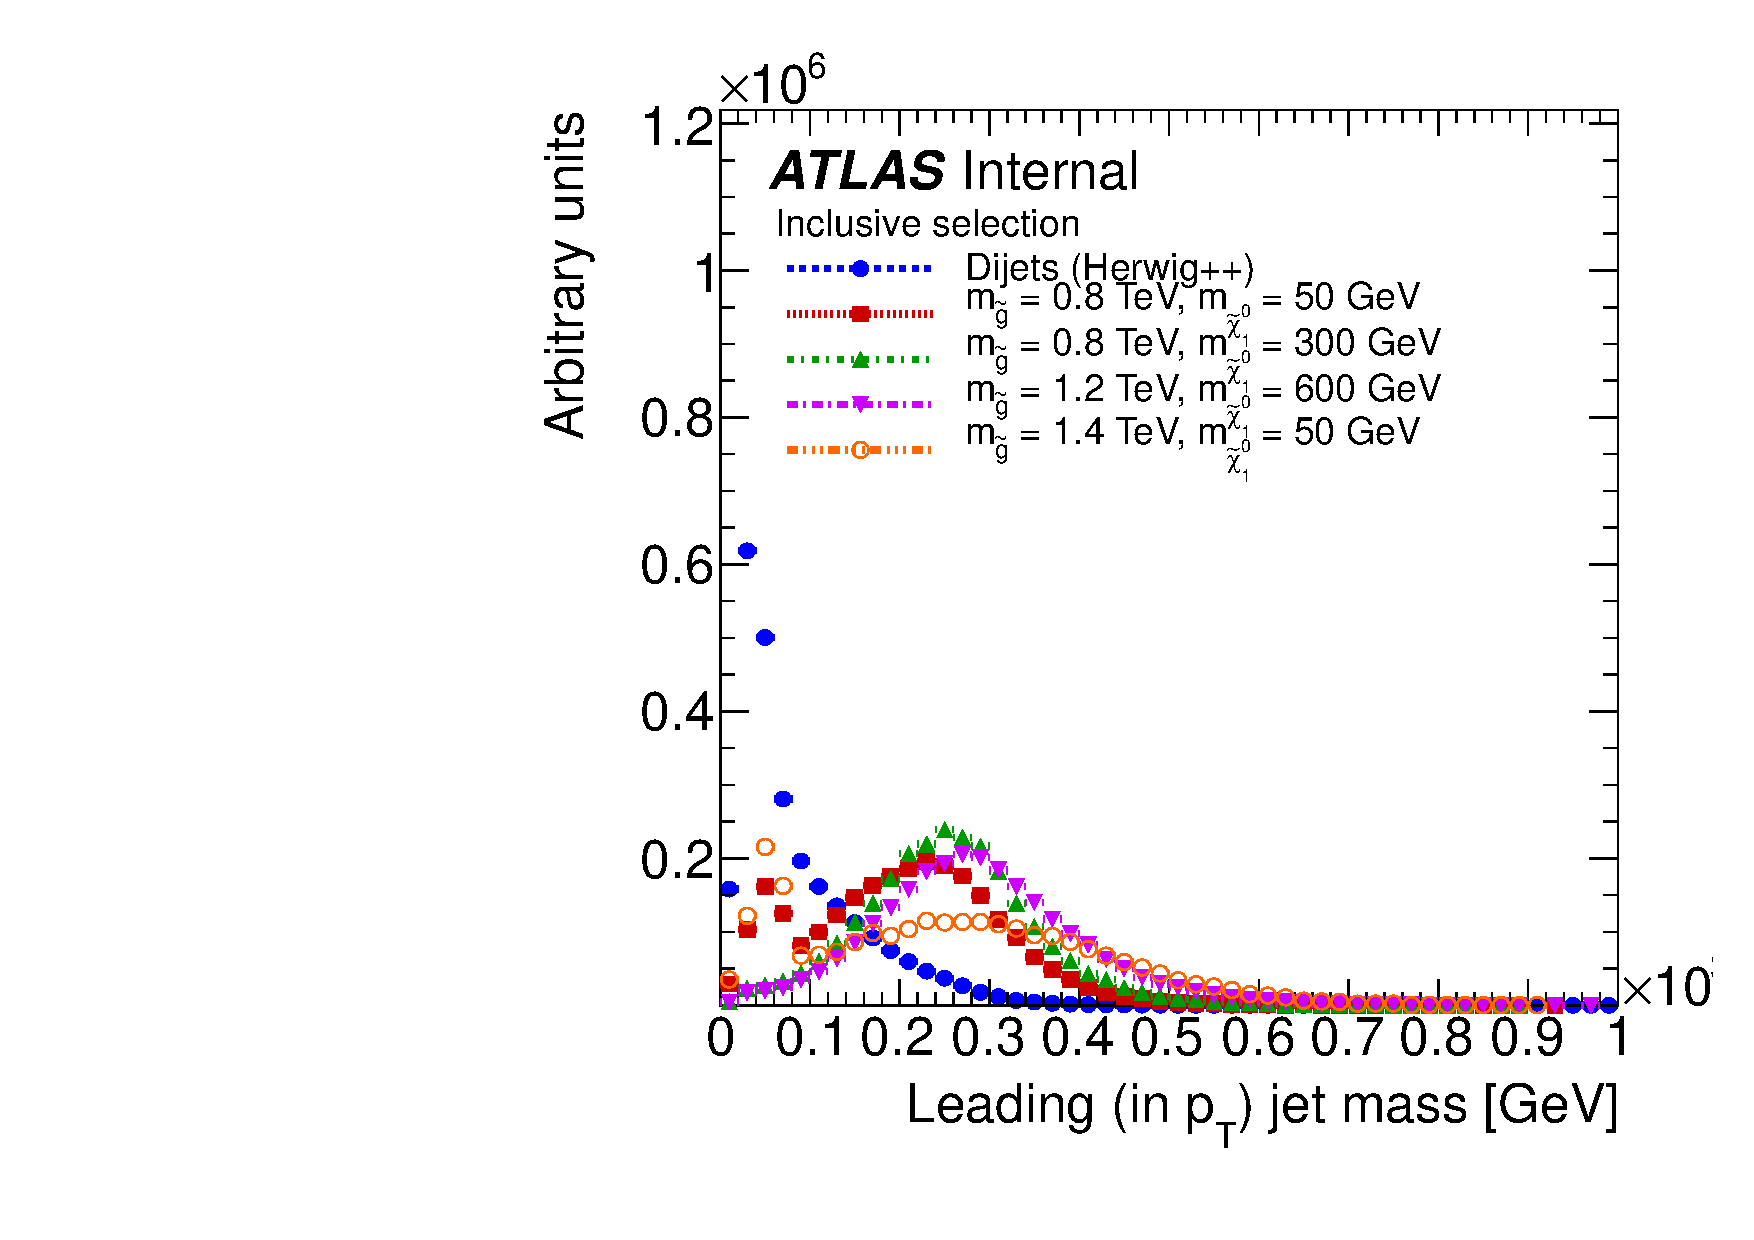
\includegraphics[width=0.45\columnwidth]{INT/Discrimination/overlay_jet_mass1_signalComparison_highBoost_Incl_j470_AntiKt10LCTopoTrimmedPtFrac5SmallR30_data12_v22.pdf}
    \label{fig:search:search:optimization:signalcomp1:highboost}}~
  \subfigure[High $\mgluino$ mass points]{
    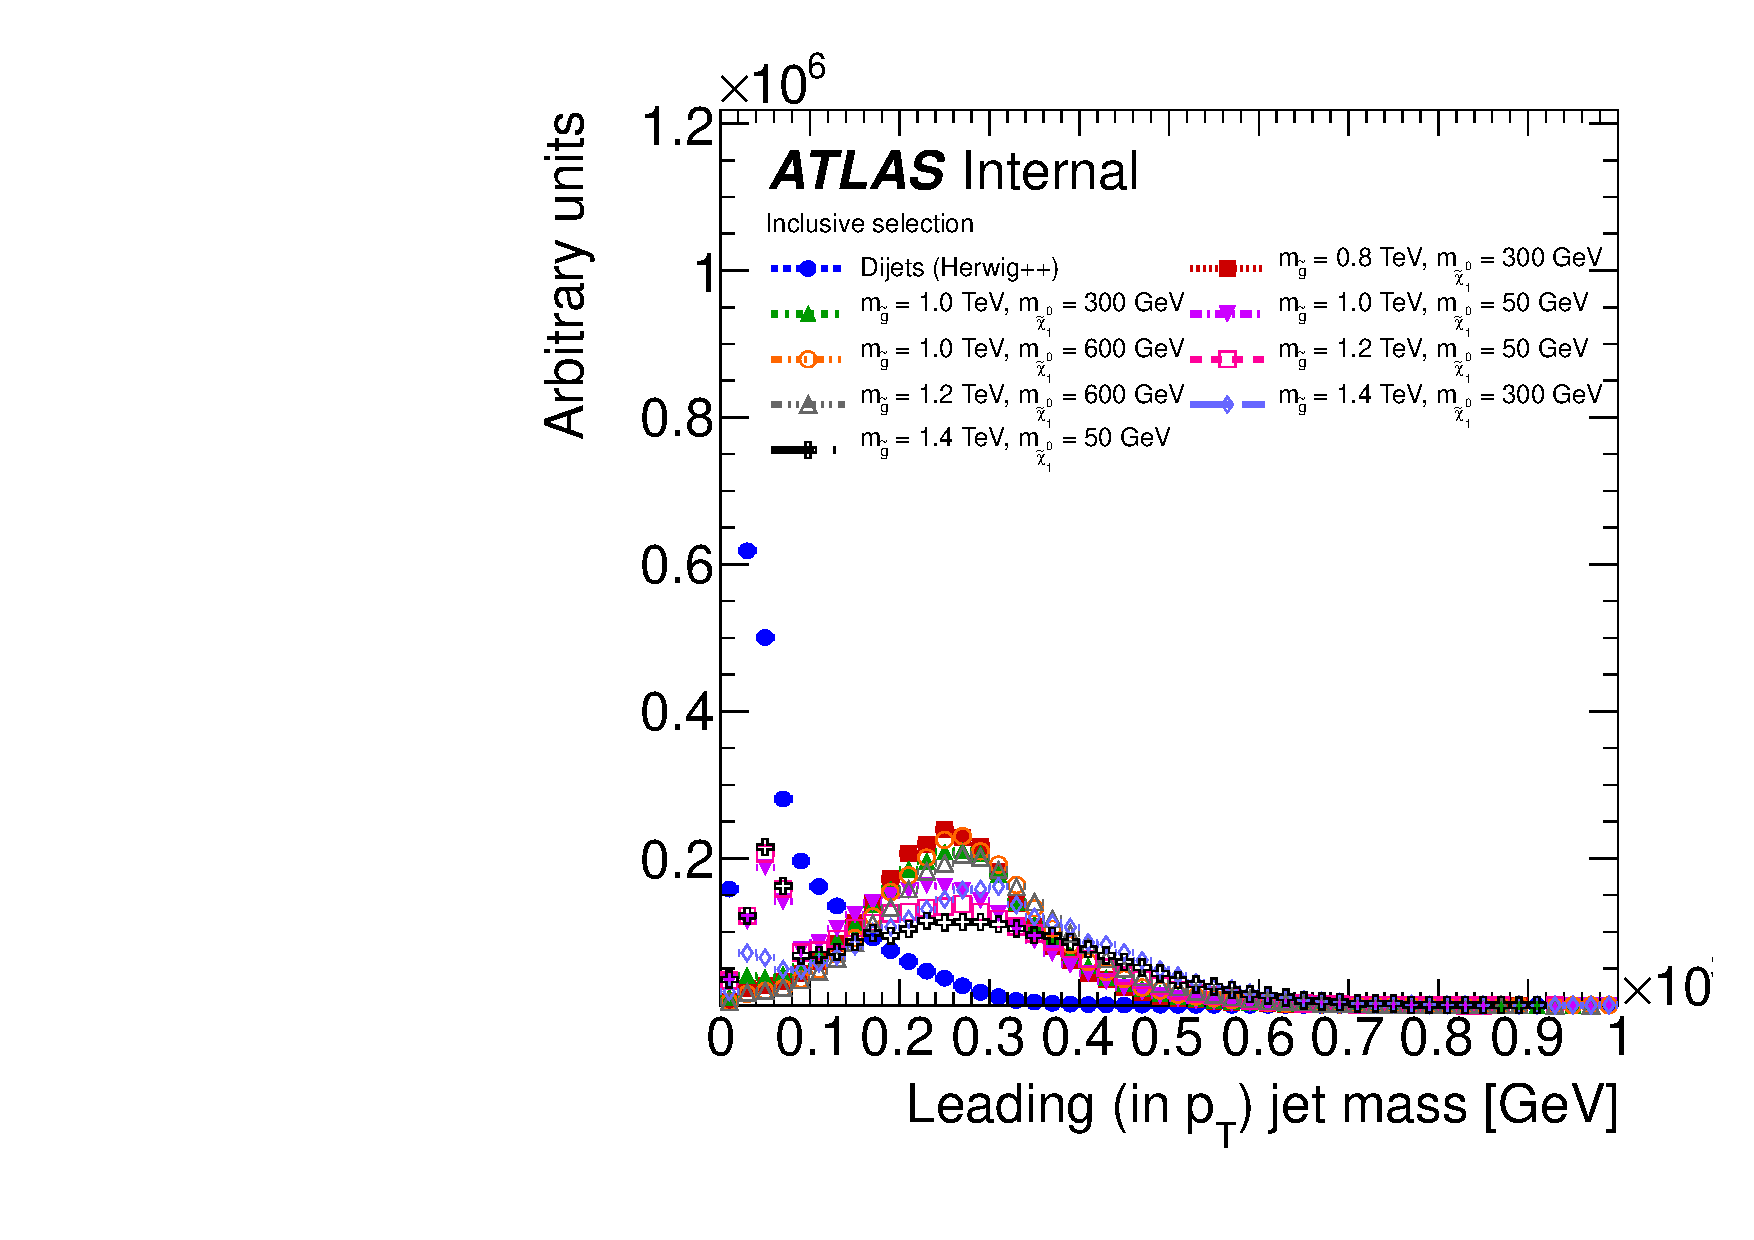
\includegraphics[width=0.45\columnwidth]{INT/Discrimination/overlay_jet_mass1_signalComparison_highGluinoM_Incl_j470_AntiKt10LCTopoTrimmedPtFrac5SmallR30_data12_v22.pdf}
    \label{fig:search:search:optimization:signalcomp1:highmg}}
  \subfigure[$\mgluino = 1$ TeV mass points]{
    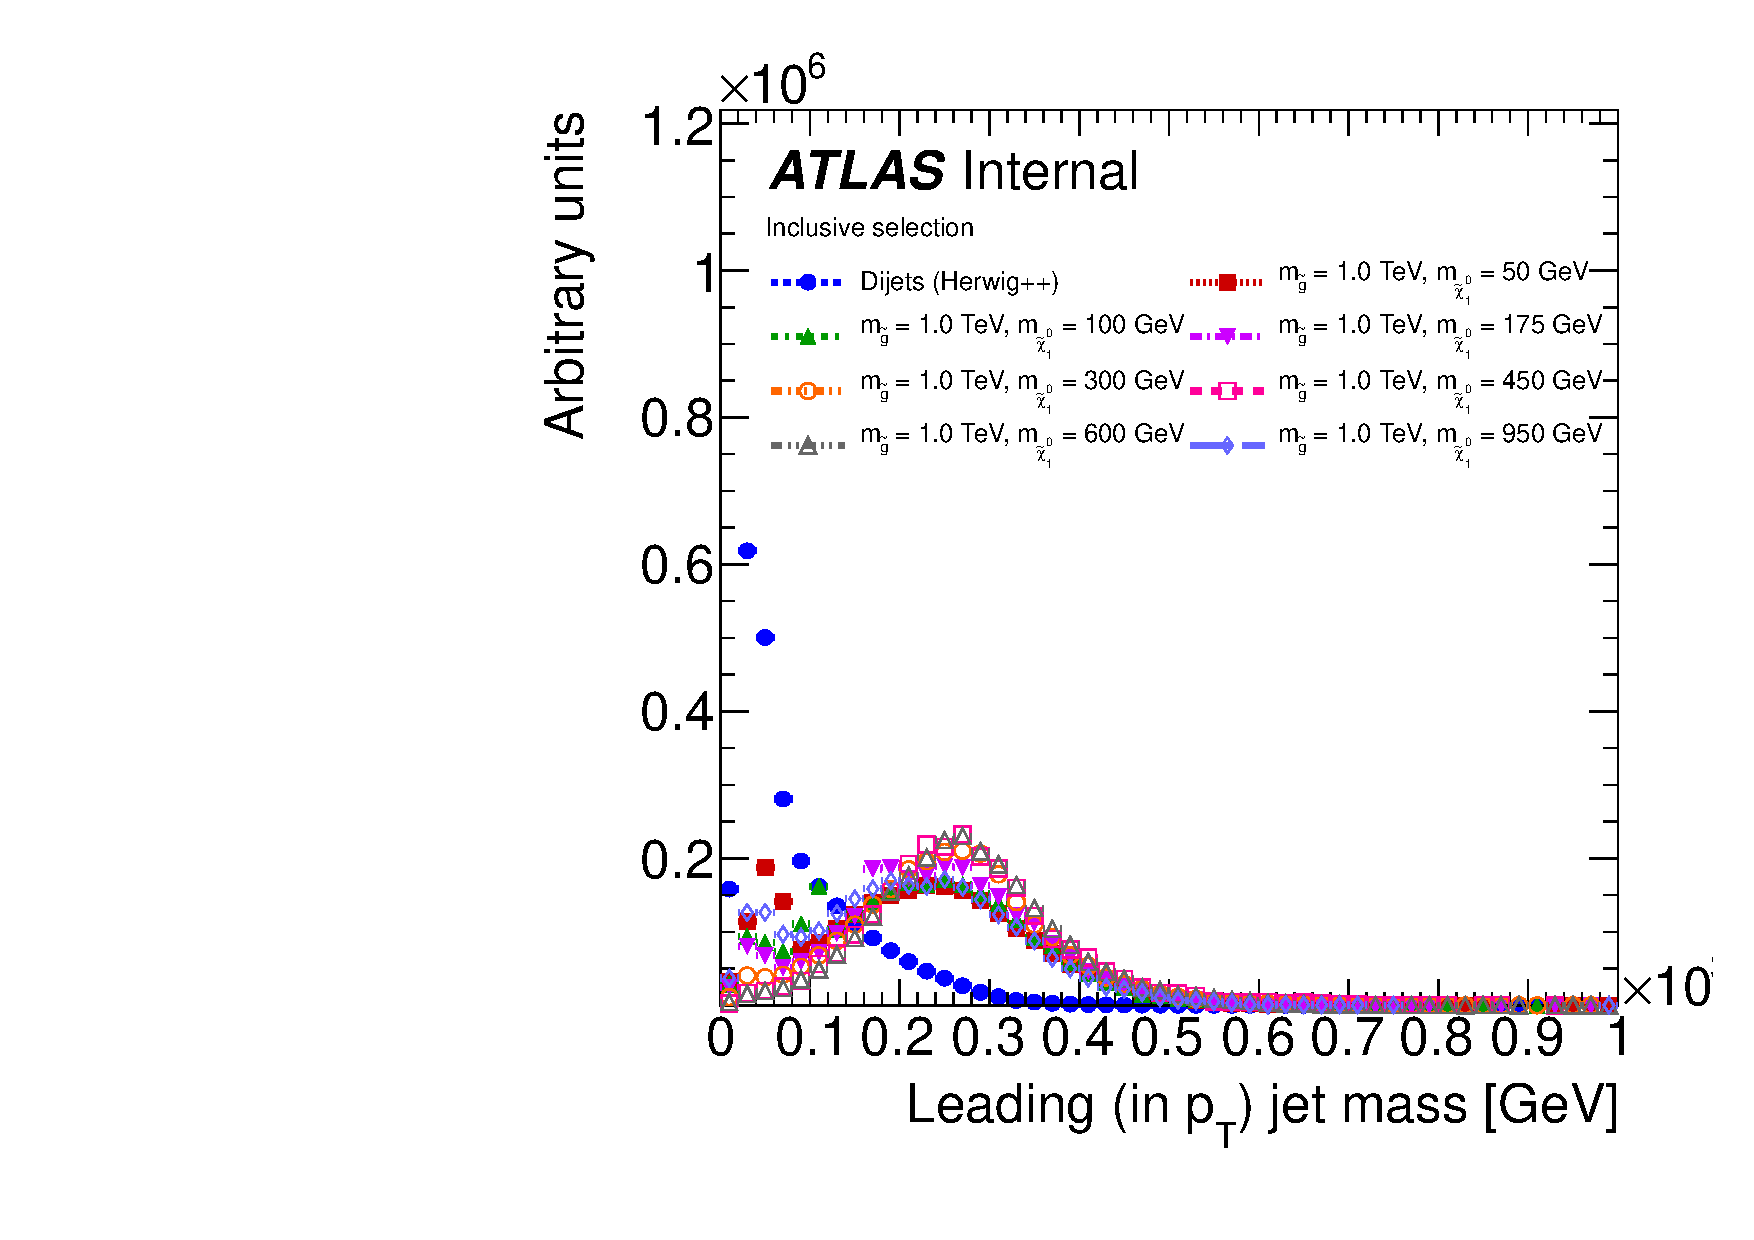
\includegraphics[width=0.45\columnwidth]{INT/Discrimination/overlay_jet_mass1_signalComparison_OneTeV_Incl_j470_AntiKt10LCTopoTrimmedPtFrac5SmallR30_data12_v22.pdf}~
    \label{fig:search:search:optimization:signalcomp1:tevmg}}
  \subfigure[$\sim$Top mass points]{
    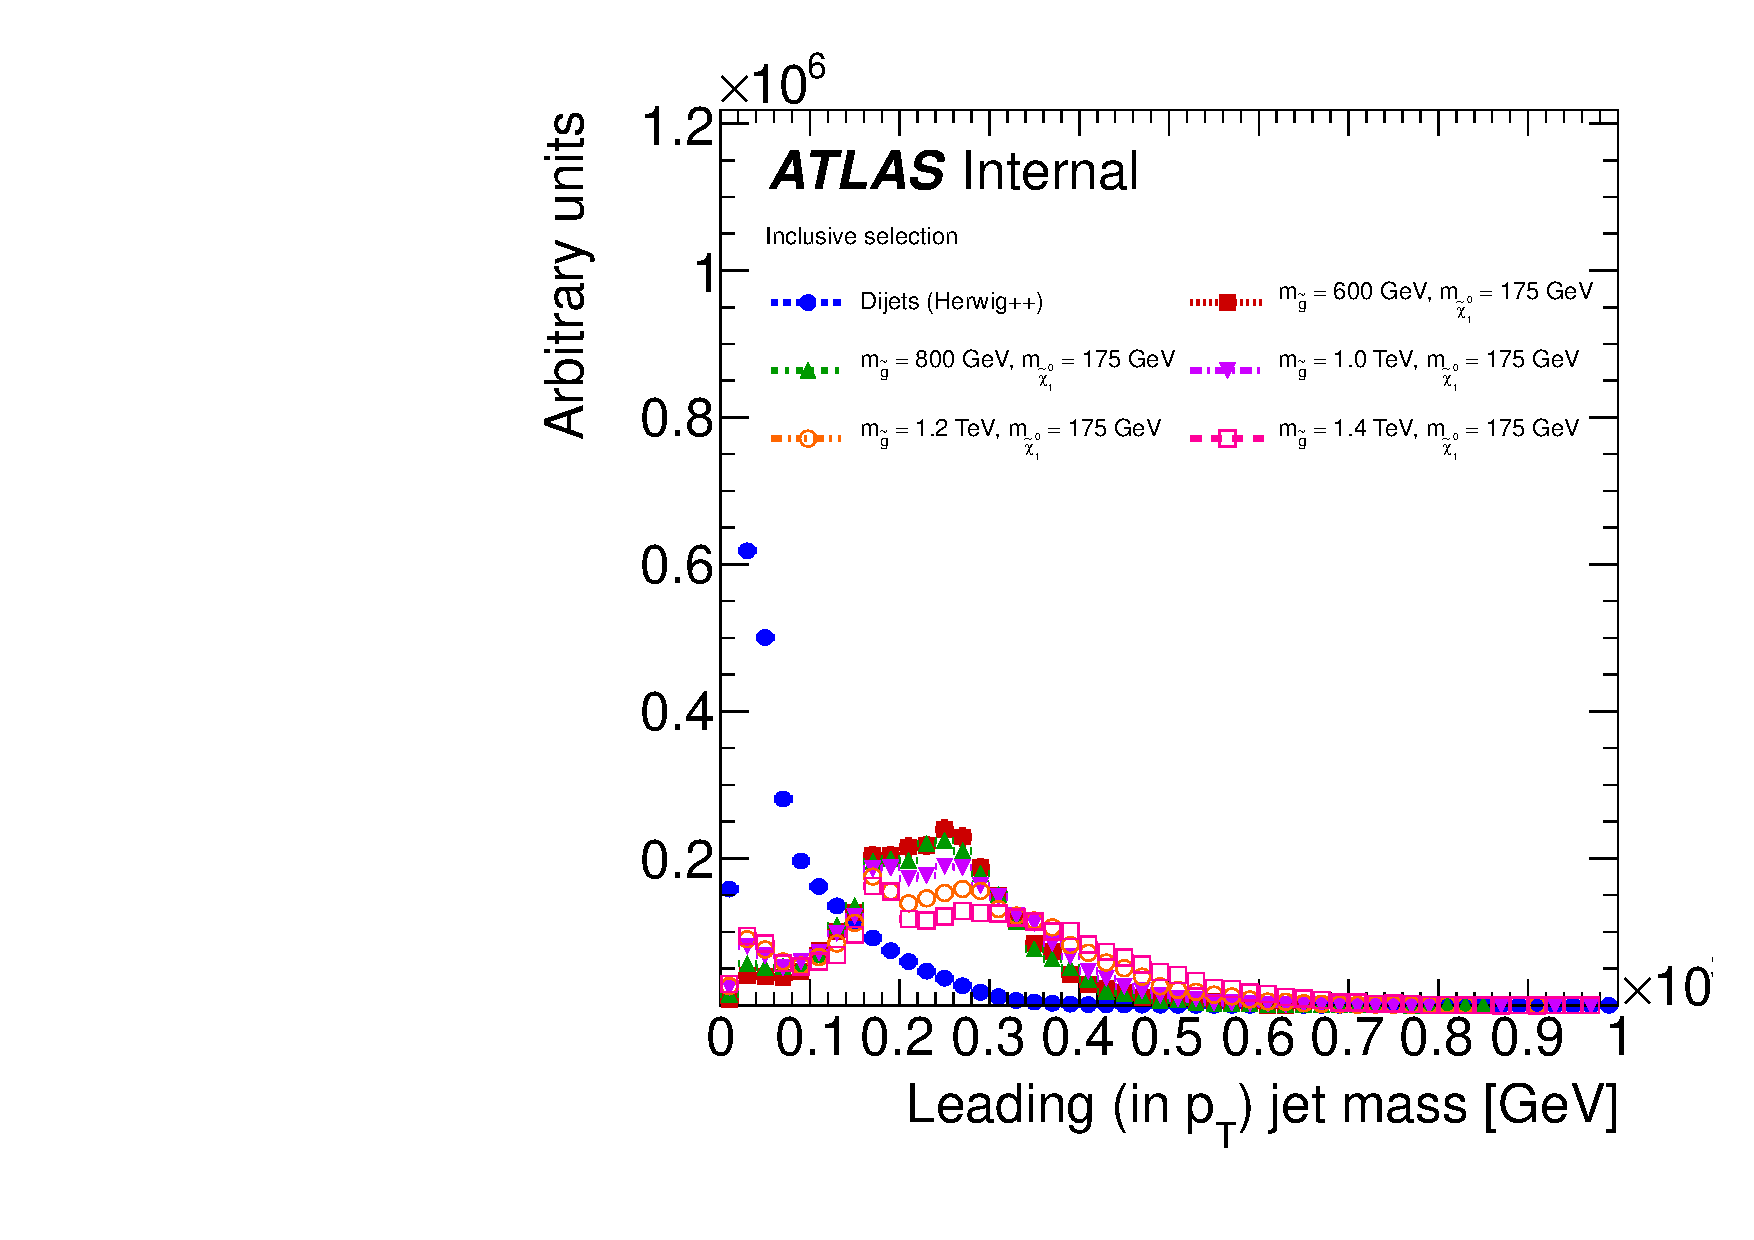
\includegraphics[width=0.45\columnwidth]{INT/Discrimination/overlay_jet_mass1_signalComparison_TopMass_Incl_j470_AntiKt10LCTopoTrimmedPtFrac5SmallR30_data12_v22.pdf}~
    \label{fig:search:search:optimization:signalcomp1:topmg}}

    
  \caption{Leading jet mass distributions for many different signal mass points, compared to the \texttt{Herwig++} dijet background. 
           }
           
  \label{fig:search:search:optimization:signalcomp1}
\end{figure}

%%------------------------------    

\begin{figure}[!ht]
  \centering
  
  \subfigure[High boost mass points.]{
    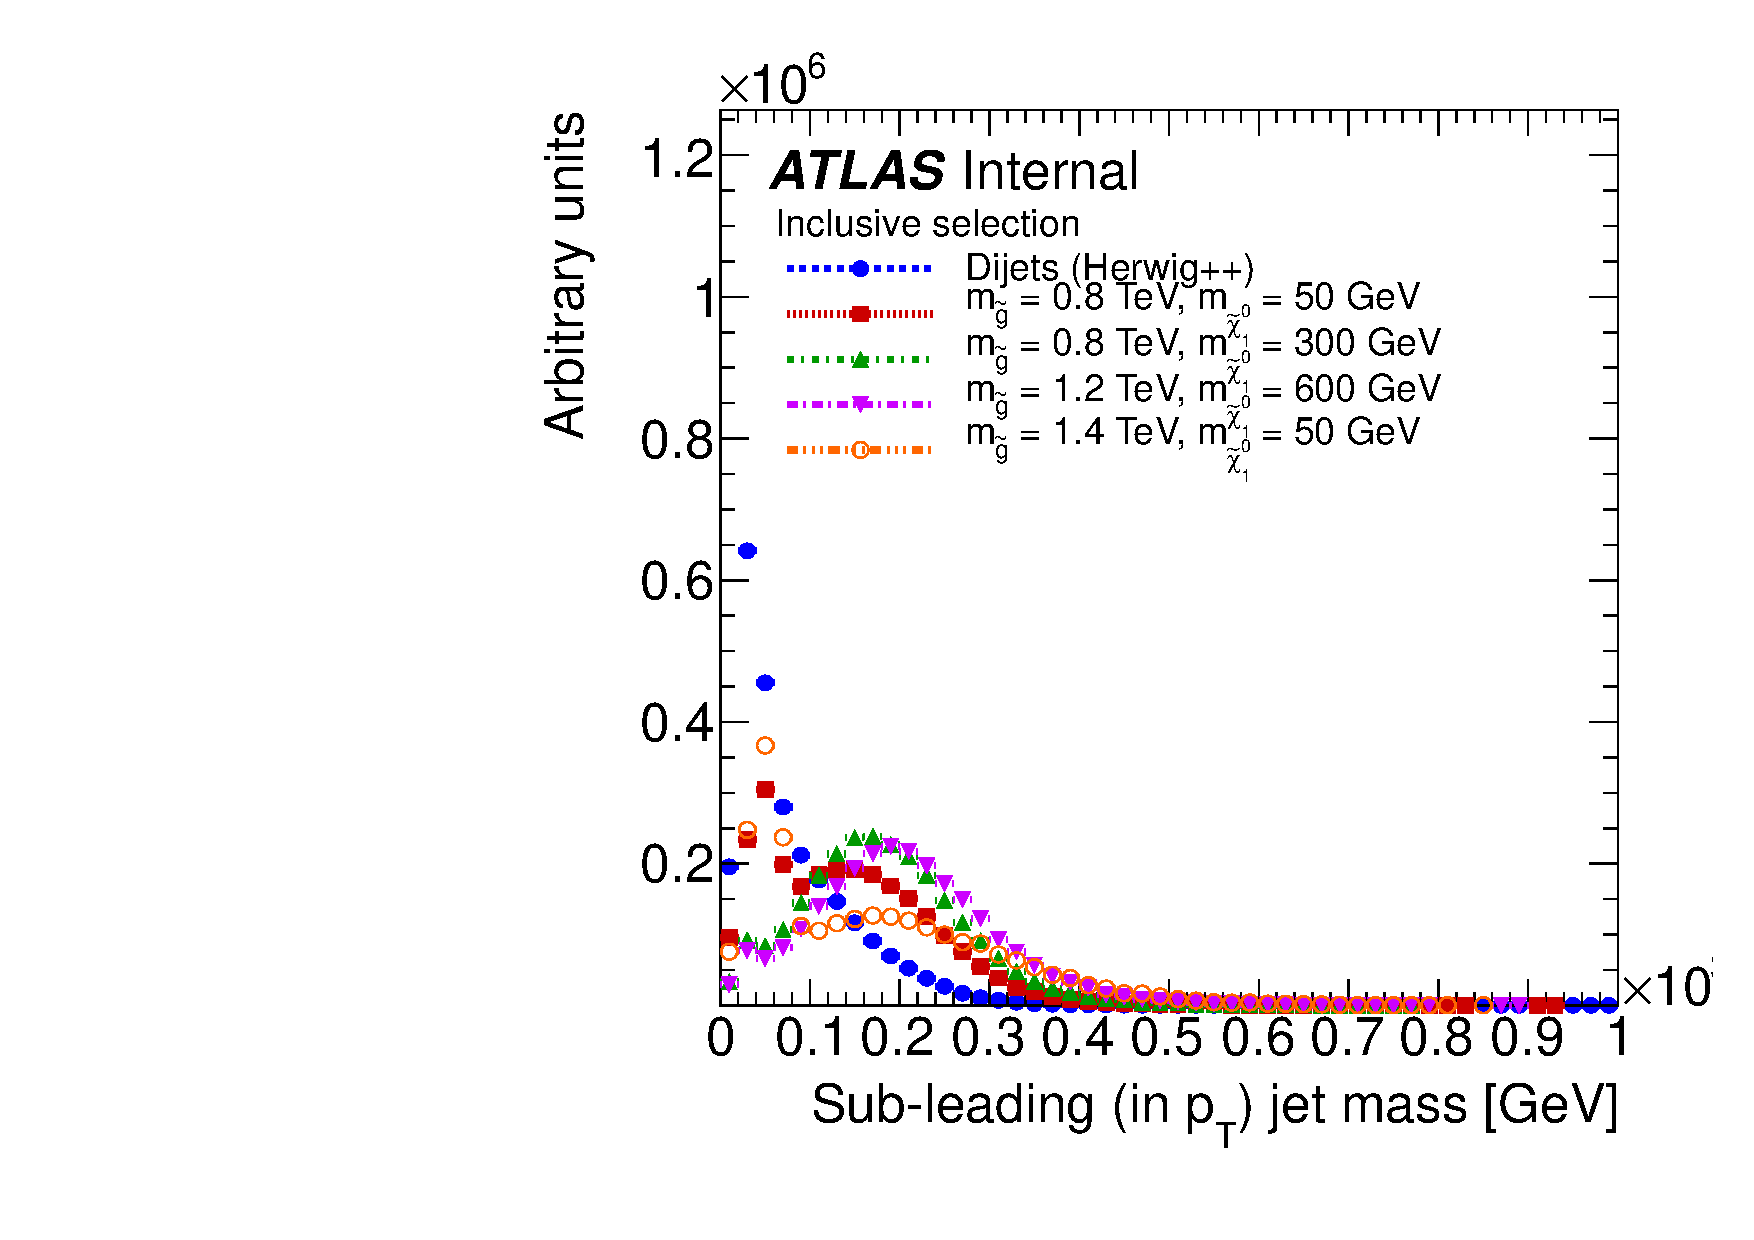
\includegraphics[width=0.45\columnwidth]{INT/Discrimination/overlay_jet_mass2_signalComparison_highBoost_Incl_j470_AntiKt10LCTopoTrimmedPtFrac5SmallR30_data12_v22.pdf}
    \label{fig:search:search:optimization:signalcomp2:highboost}}~
  \subfigure[High $\mgluino$ mass points]{
    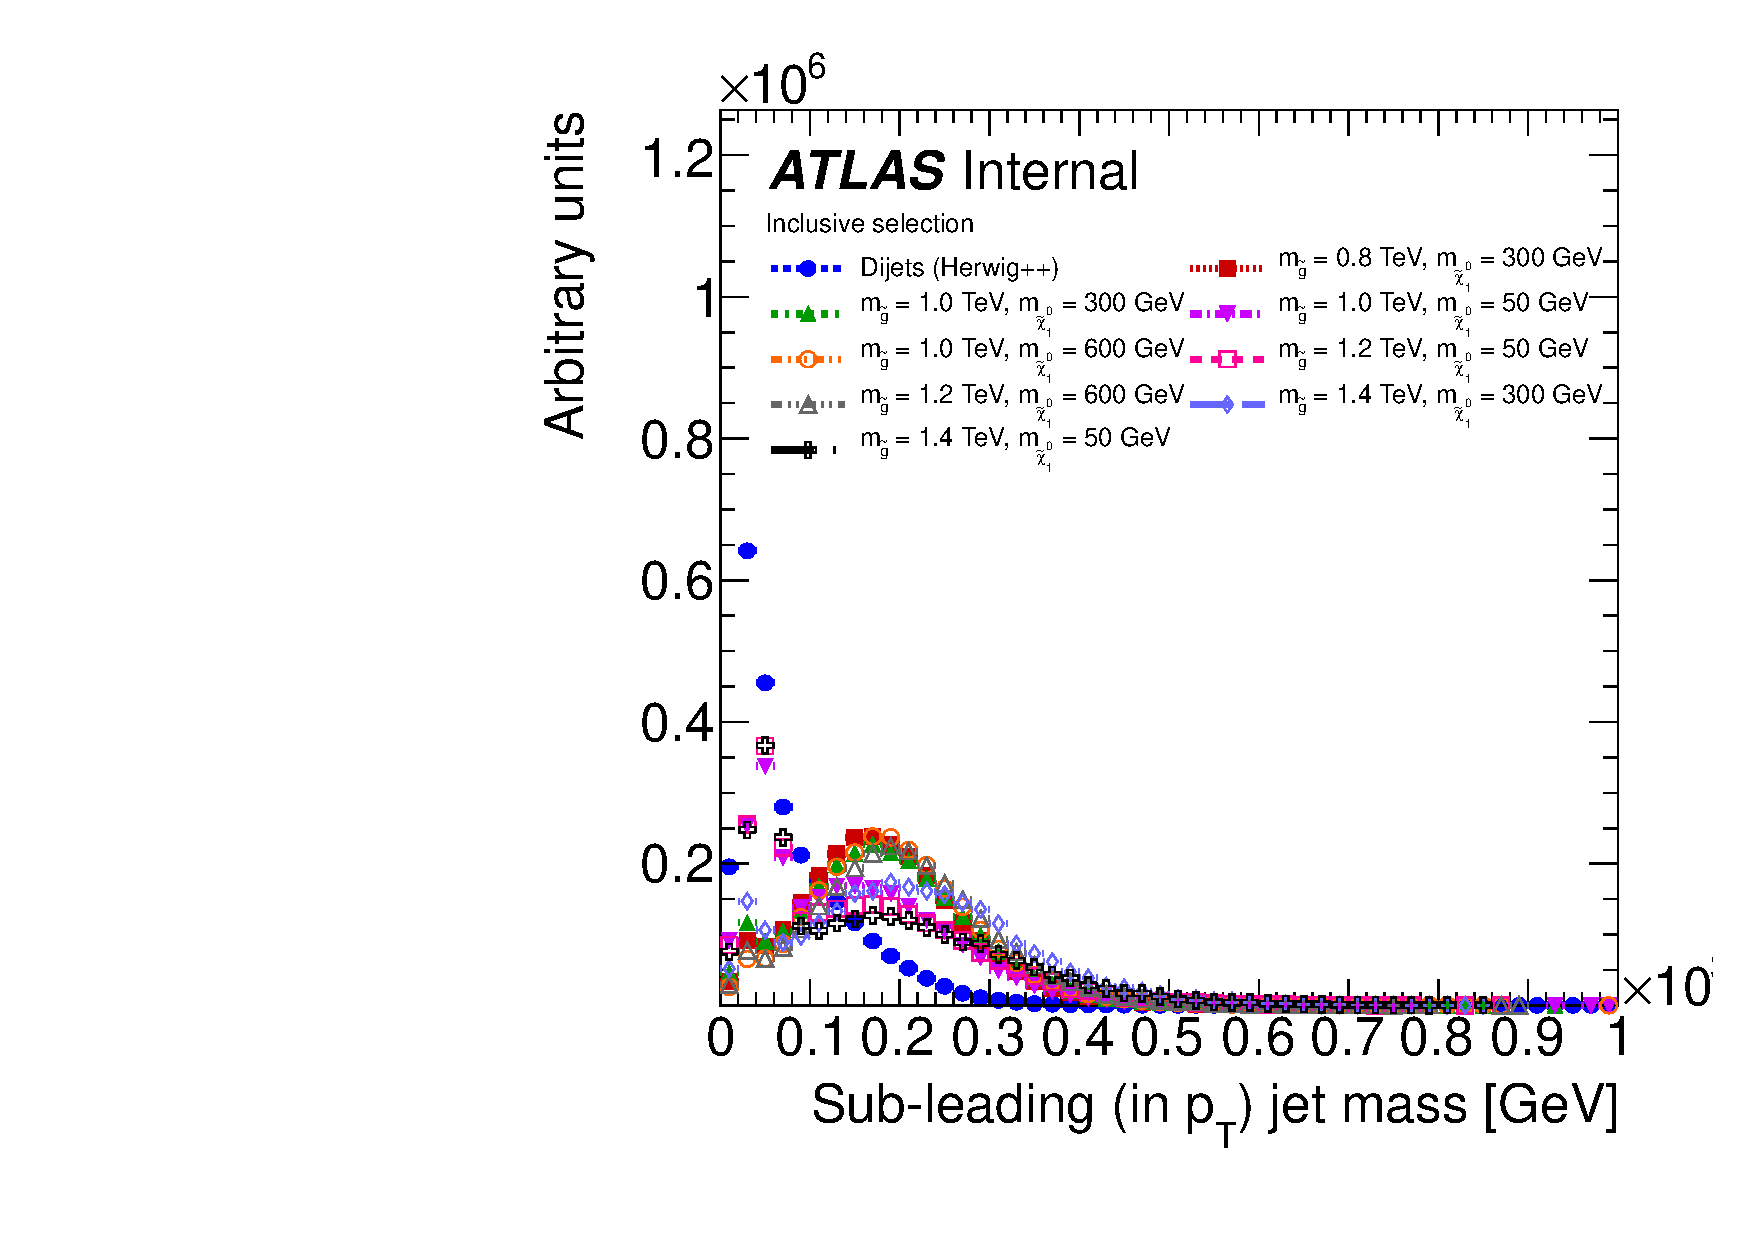
\includegraphics[width=0.45\columnwidth]{INT/Discrimination/overlay_jet_mass2_signalComparison_highGluinoM_Incl_j470_AntiKt10LCTopoTrimmedPtFrac5SmallR30_data12_v22.pdf}
    \label{fig:search:search:optimization:signalcomp2:highmg}}
  \subfigure[$\mgluino = 1$ TeV mass points]{
    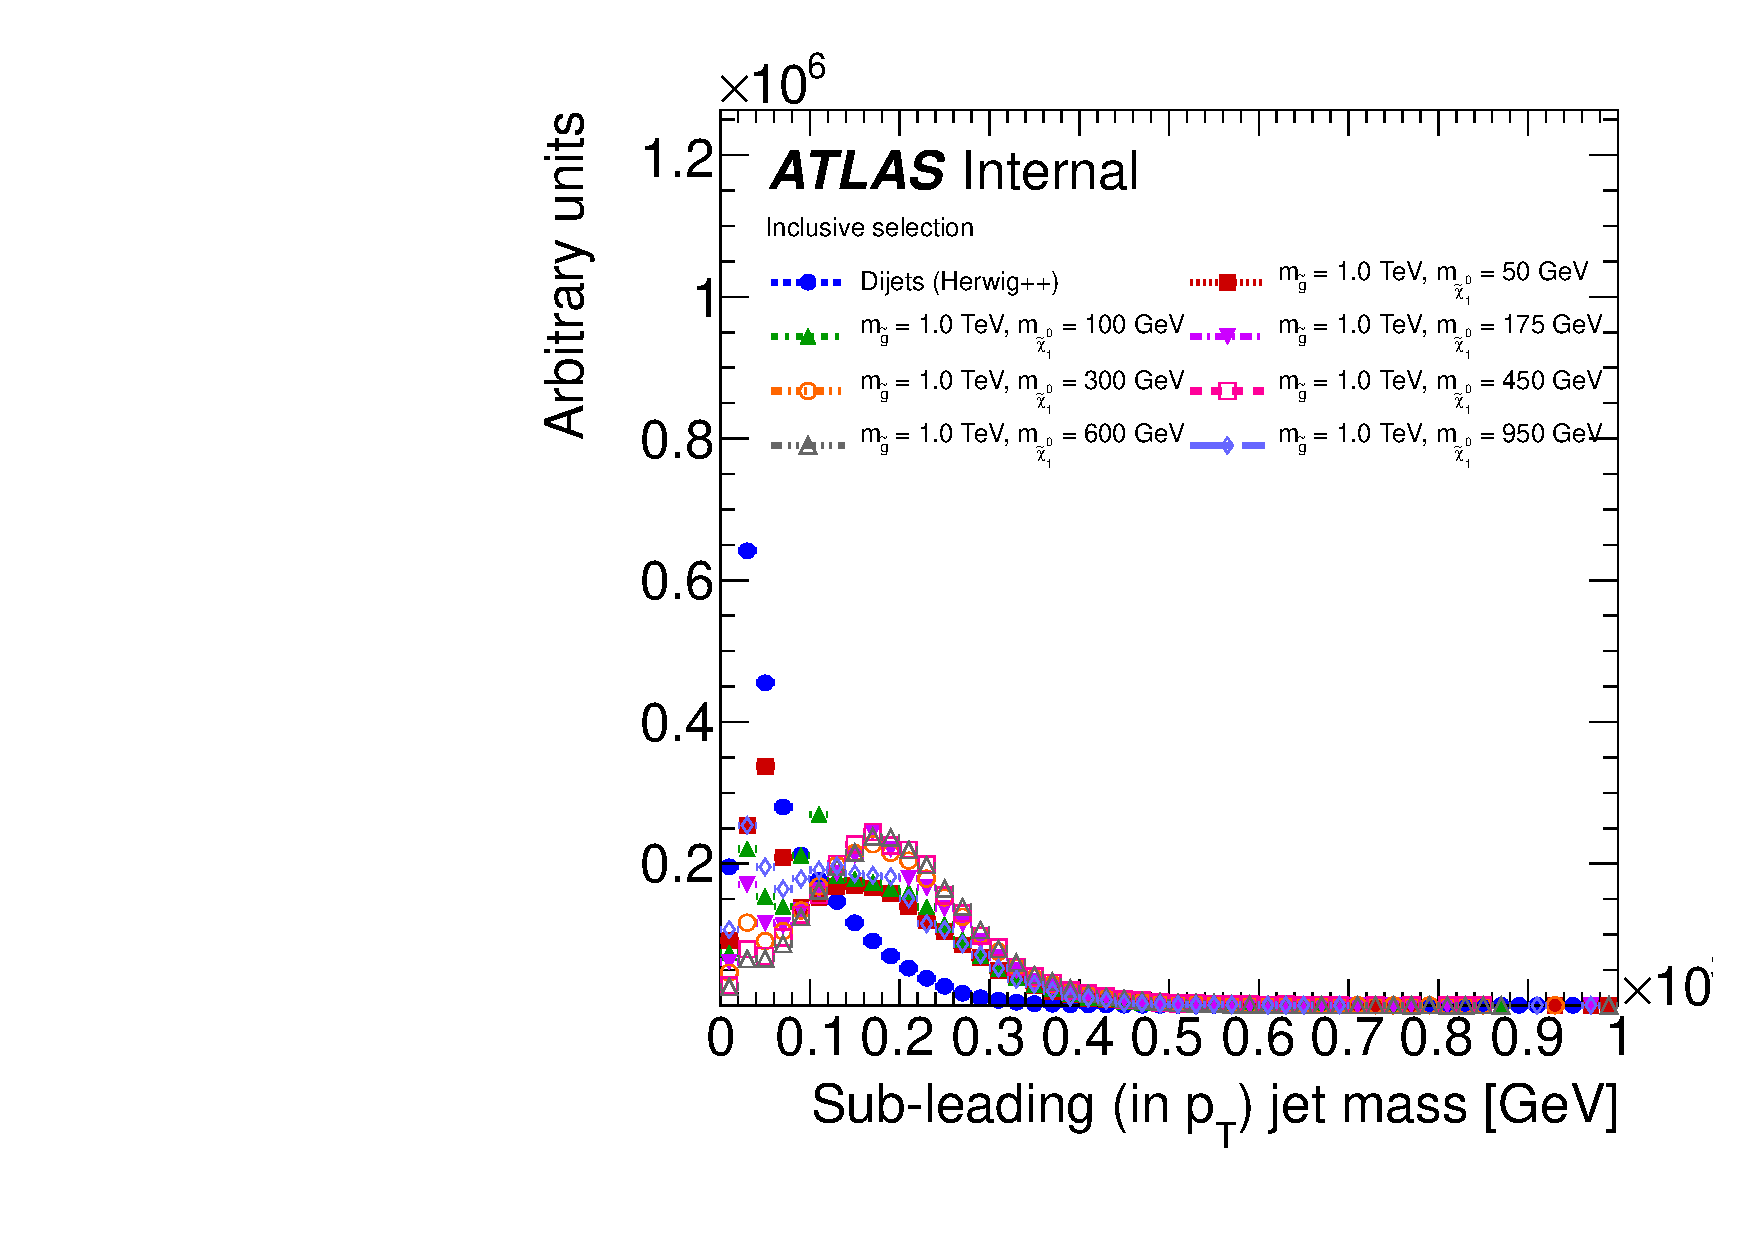
\includegraphics[width=0.45\columnwidth]{INT/Discrimination/overlay_jet_mass2_signalComparison_OneTeV_Incl_j470_AntiKt10LCTopoTrimmedPtFrac5SmallR30_data12_v22.pdf}~
    \label{fig:search:search:optimization:signalcomp2:tevmg}}
  \subfigure[$\sim$Top mass points]{
    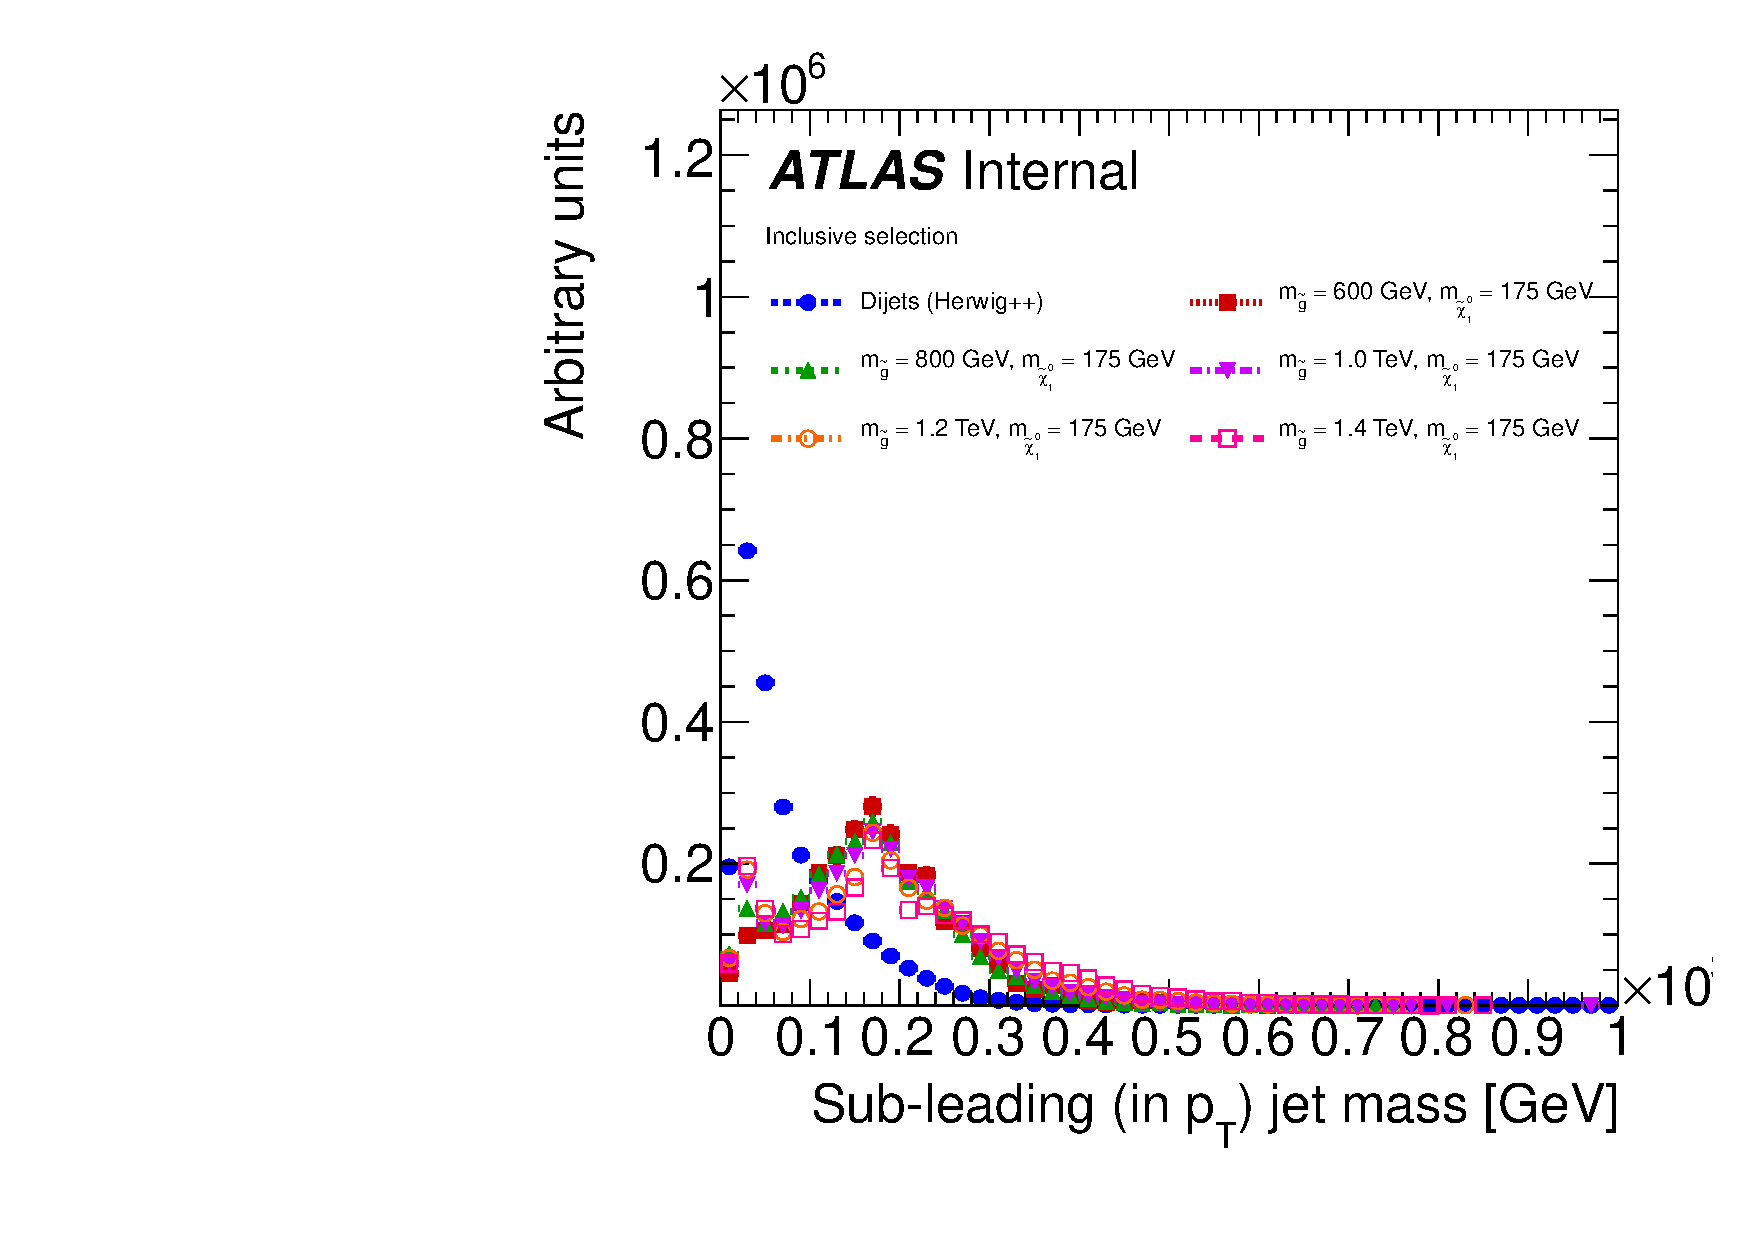
\includegraphics[width=0.45\columnwidth]{INT/Discrimination/overlay_jet_mass2_signalComparison_TopMass_Incl_j470_AntiKt10LCTopoTrimmedPtFrac5SmallR30_data12_v22.pdf}~
    \label{fig:search:search:optimization:signalcomp2:topmg}}

    
  \caption{Subleading jet mass distributions for many different signal mass points, compared to the \texttt{Herwig++} dijet background. 
           }
           
  \label{fig:search:search:optimization:signalcomp2}
\end{figure}

%%------------------------------    

Finally, while our main goal is to study the \gluino-\lsp model inclusively in flavor, it is interesting to consider whether we are particularly sensitive, for example, to \gluino decays mediated through $\tilde{t}$, or whether we are pick out mostly \lsp decays to $\tilde{t}$. In principle, top decays should slightly increase the quark multiplicity, as leptonic decays produce only one quark and hadronic decays produce three. While it is difficult to tell because of the limited statistics in the flavor-sliced samples, Figure~\ref{fig:search:search:optimization:flavor} shows the difference between situations in which the \gluino or \lsp decay to tops, compared to an inclusive sample. Both the \MJ and leading jet mass are approximately consistent over these comparisons, showing that the analysis selects flavor without large amounts of bias.


%%------------------------------
\begin{figure}[!ht]
  \centering

  \subfigure[Jet $M_{J,4}^{\Sigma}$]{
    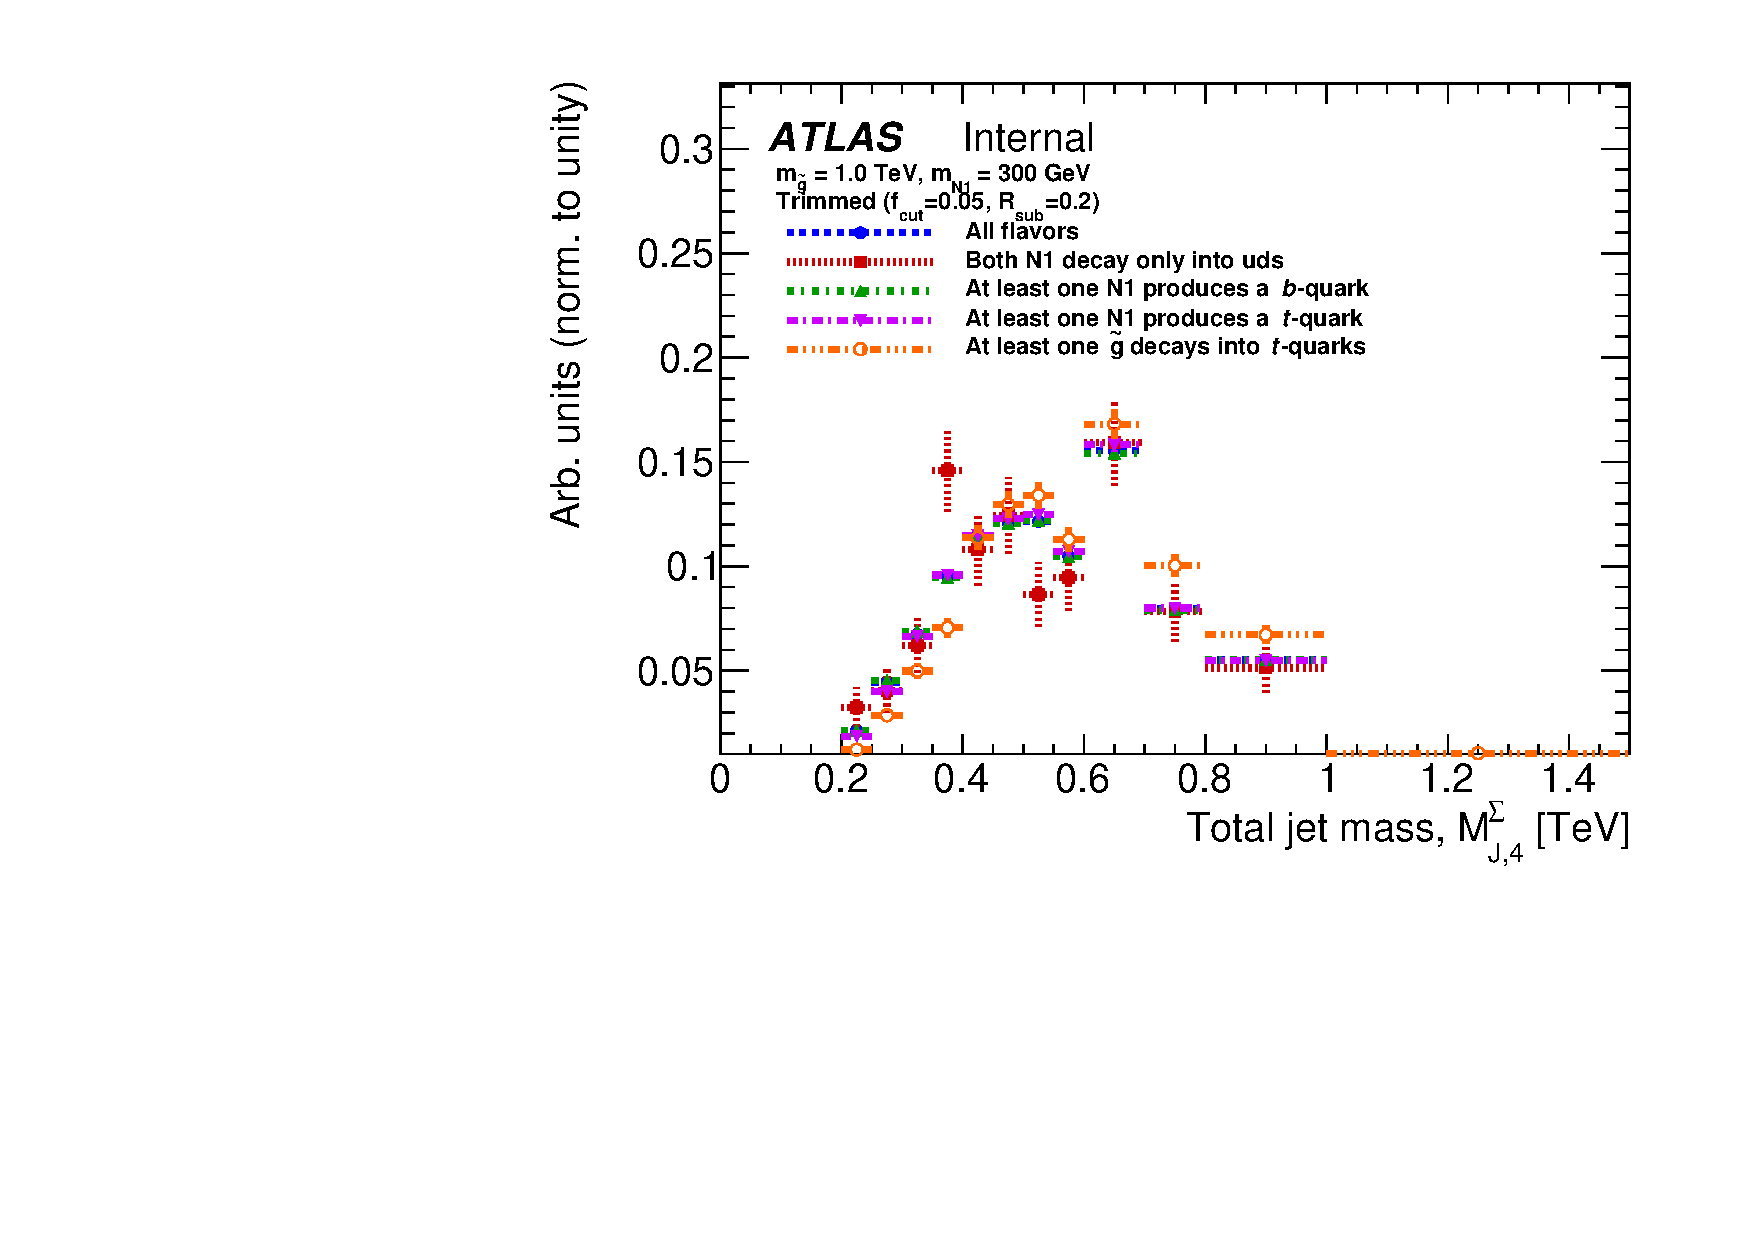
\includegraphics[width=0.48\textwidth]{INT/FlavorStudies/overlay_MJ4_jetComparison_all_AntiKt10LCTopoTrimmedPtFrac5SmallR30_Trimmed.pdf}
    \label{fig:search:search:optimization:flavor:mj4}}
  \subfigure[Jet $m_{j,1}$]{
    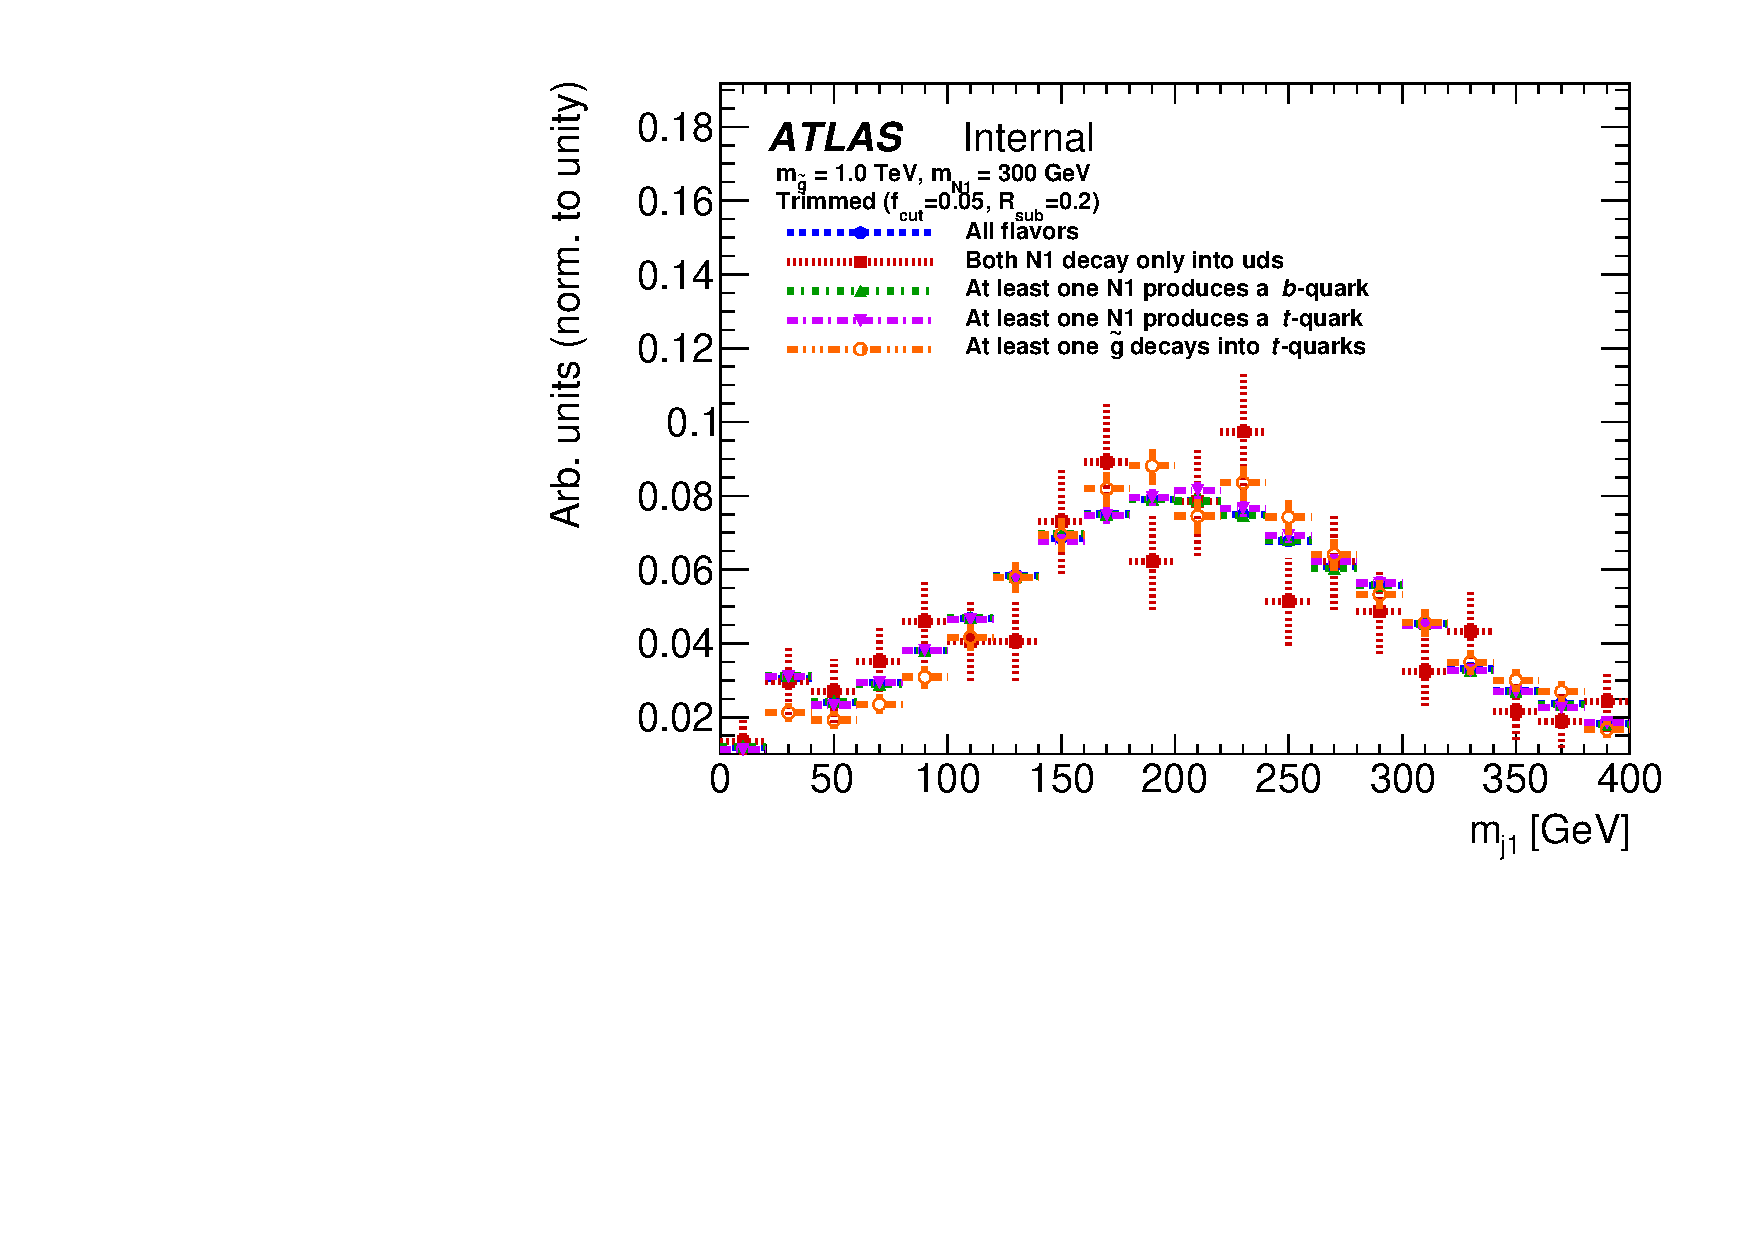
\includegraphics[width=0.48\textwidth]{INT/FlavorStudies/overlay_jet_mass1_jetComparison_all_AntiKt10LCTopoTrimmedPtFrac5SmallR30_Trimmed.pdf}
    \label{fig:search:search:optimization:flavor:m1}}
  
    \caption{Mass distributions for different truth particle final state flavors. The shape of the distributions was shown to be approximately independent of the final state.}
  \label{fig:search:search:optimization:flavor}
\end{figure}
%%------------------------------

\subsubsection{Two-Dimensional Optimization}

The second phase of optimization involves deciding on variable to be used in combination with \MJ. Additionally, as this second variable is meant to determine the creation of signal and control regions, it should not be strongly correlated with \MJ: large correlations could bias the information determined in a control region, such that it would not be directly applicable to a signal region anymore.

The easiest way to see the differences between pairs of variables is to construct two dimensional likelihoods, defining:
%
\begin{equation}
L = \frac{S}{S+B}
\end{equation}
%
where $S$ and $B$ are two-dimensional histograms in the two variables of interest, separately for signal and background. A useful pair of variables will have a high $L$ in a corner of this space: this would indicate that both variables are useful, and that they provide complementary information. Highly correlated variables appear as a line: this indicates that the power of one variable is strongly associated to a second, and that a cut on only one of them would be sufficient. 

Figure~\ref{fig:search:search:optimization:2D:NCA} and \ref{fig:search:search:optimization:2D:NKT}, for example, show the likelihoods formed with the subjet counting variables. While $N_{CA}$ and $N_{kT}$ are useful on their own, they provide little information on top of $\MJ$: a horizontal cut in this plane would provide just as much power as a diagonal (or curved) cut. The correlation levels in the background between \MJ and these variables is over $60\%$, indicating that indeed little additional information is contained. $T_{32}$ and $T_{21}$ are also similarly correlated to \MJ, and therefore are also not particularly useful.


%%%%%%%%%%%%%%%%

\begin{figure}
\centering
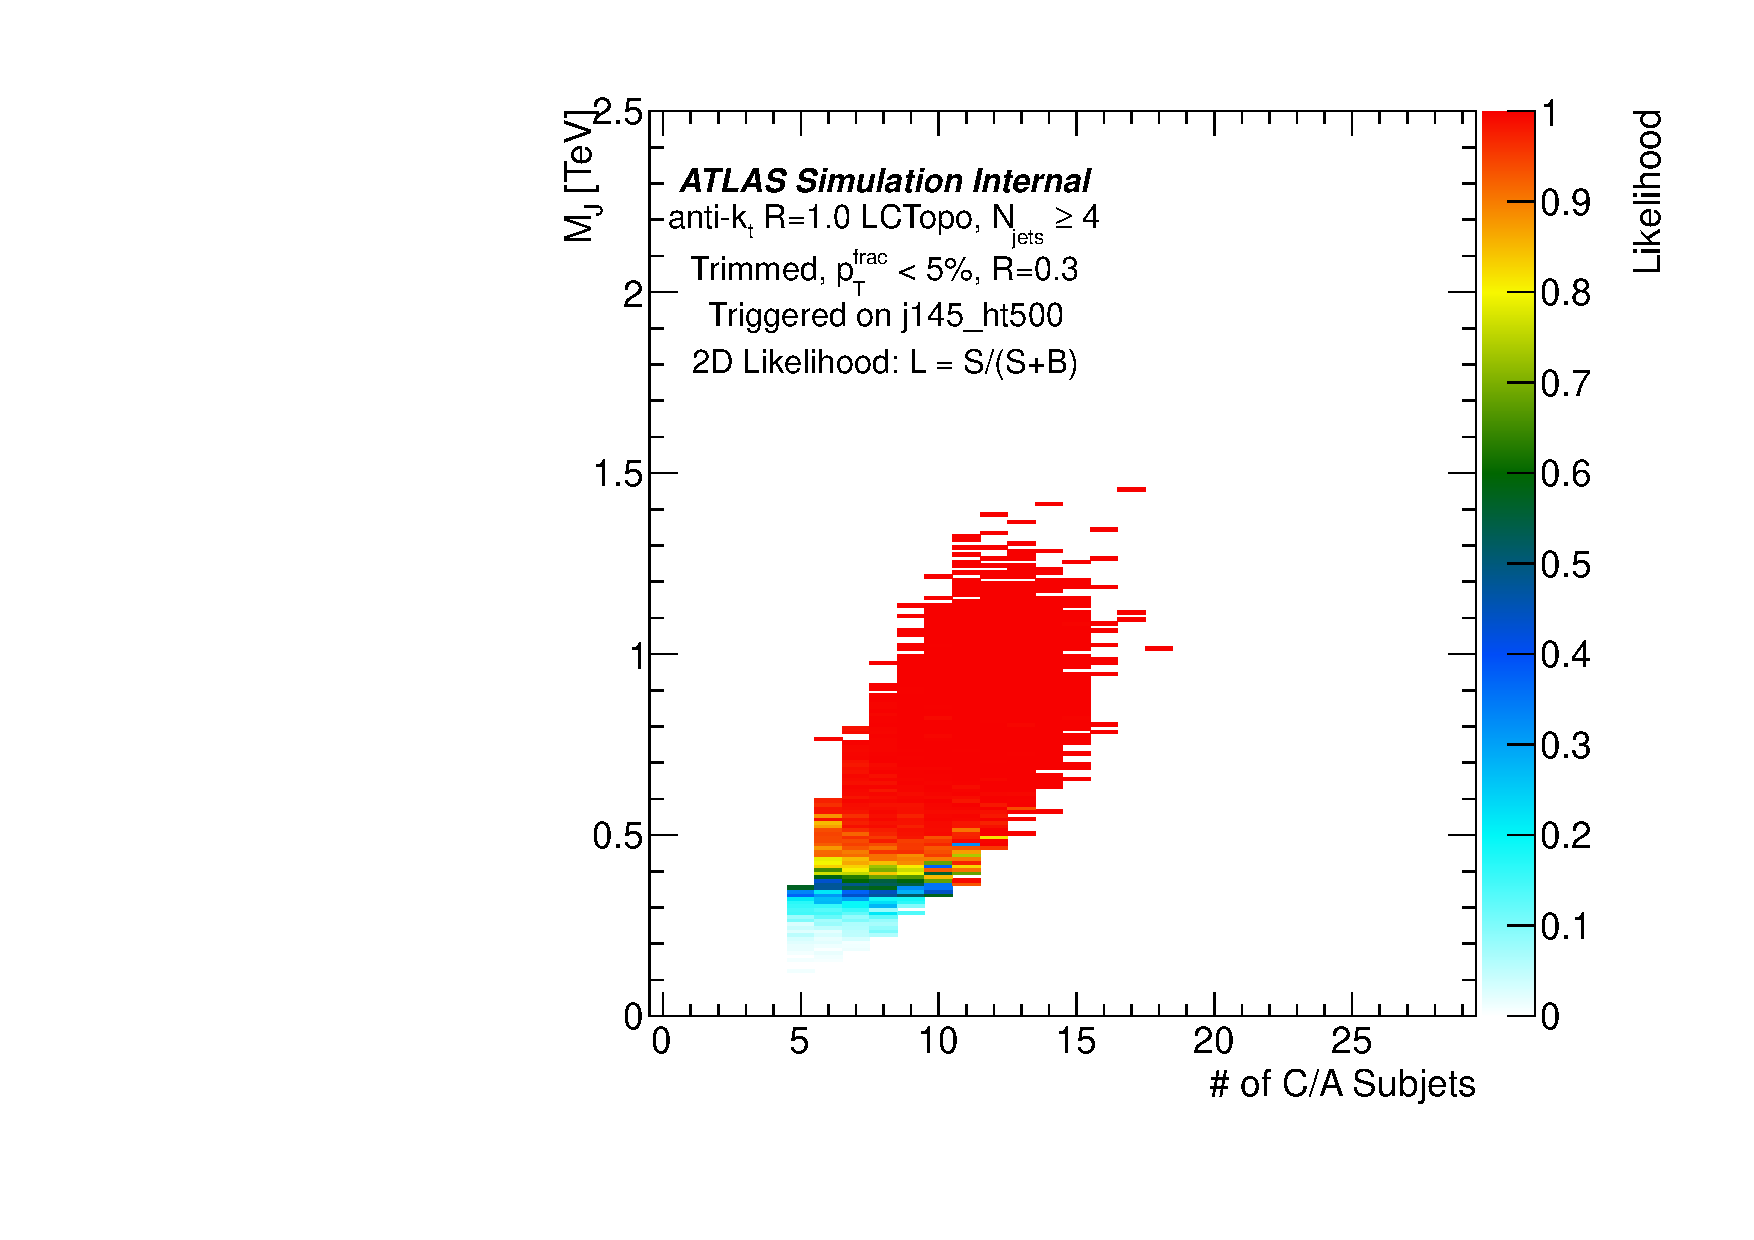
\includegraphics[width=0.5\textwidth]{INT/AntiKt10LCTopoTrimmedPtFrac5SmallR30_j145_ht500_NjetIncl_NFatJetMin4_MJ4_vs_NCASub4_SigPoint1_L_RPVGluino.pdf}
\label{fig:search:search:optimization:2D:NCA}
\caption{A likelihood for discrimination between a high $m_{\gluino}$ point and a \herwigpp di-jet background, using \MJ and $N_{CA}$ as inputs.}
\end{figure}

%%%%%%%%%%%%%%%%  


%%%%%%%%%%%%%%%%

\begin{figure}
\centering
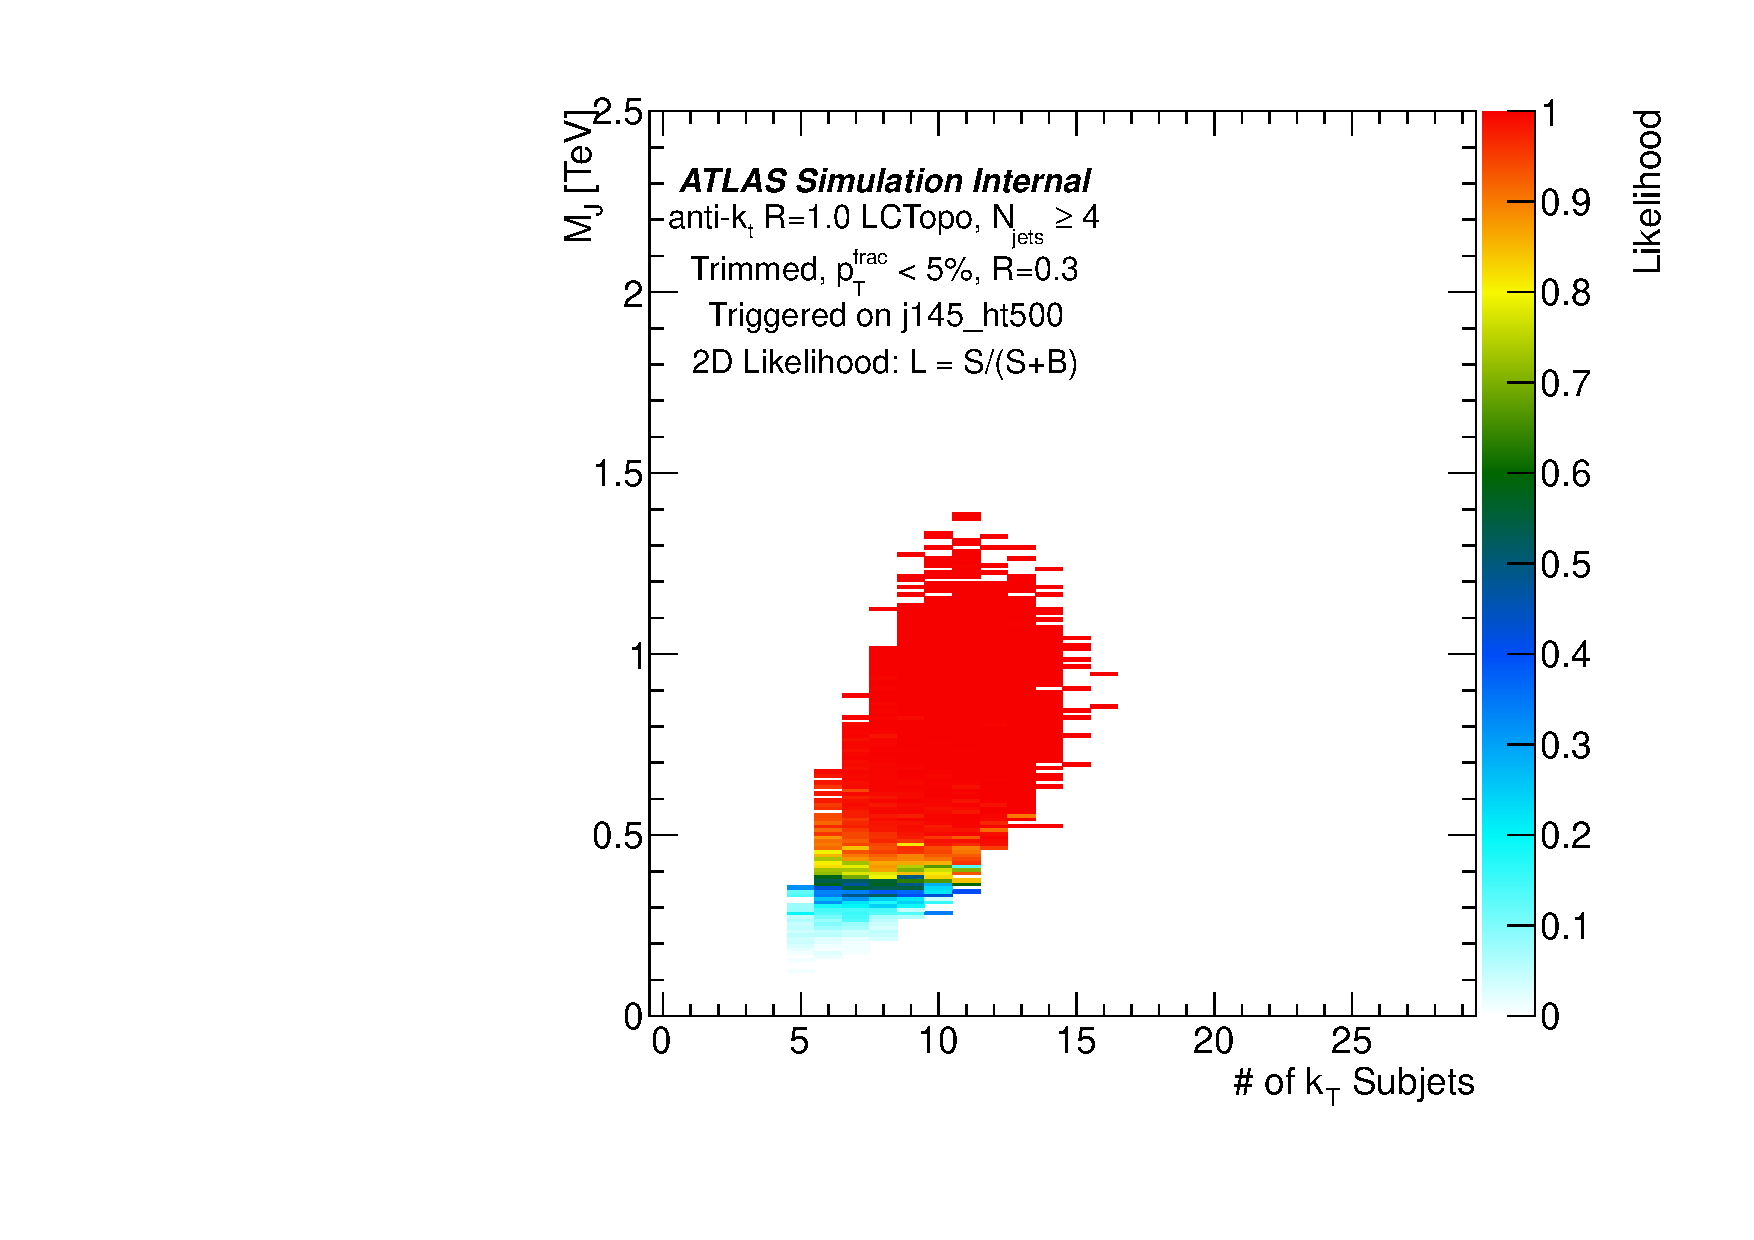
\includegraphics[width=0.5\textwidth]{INT/AntiKt10LCTopoTrimmedPtFrac5SmallR30_j145_ht500_NjetIncl_NFatJetMin4_MJ4_vs_NKTSub4_SigPoint1_L_RPVGluino.pdf}
\label{fig:search:search:optimization:2D:NKT}
\caption{A likelihood for discrimination between a high $m_{\gluino}$ point and a \herwigpp di-jet background, using \MJ and $N_{kt}$ as inputs.}
\end{figure}

%%%%%%%%%%%%%%%% 


Other variables have less correlation, and therefore potentially improved utility. Figure~\ref{fig:search:search:optimization:2D:PT31}, for example, shows the likelihood constructed with $\pt^3/\pt^1$: a diagonal cut, incorporating the discriminating power of both variables, would be clearly helpful. In this case, the correlation in the background between the two variables is at $20\%$: still substantial, but significantly reduced compared to the substructure based variables. This is reasonable, as all substructure variables are correlated to some extent: mass arises from the presence of wild angle radiation, which also causes extra subjets or lower talues of $\tau_{32}$, etc. Kinematic information like \pt is slightly correlated with masses as well, but less when looking at a ratio of \pt's, and looking at only some of the jets (instead of \Ht, which looks at the \pt of all them like much like \MJ).

%%%%%%%%%%%%%%%%

\begin{figure}
\centering
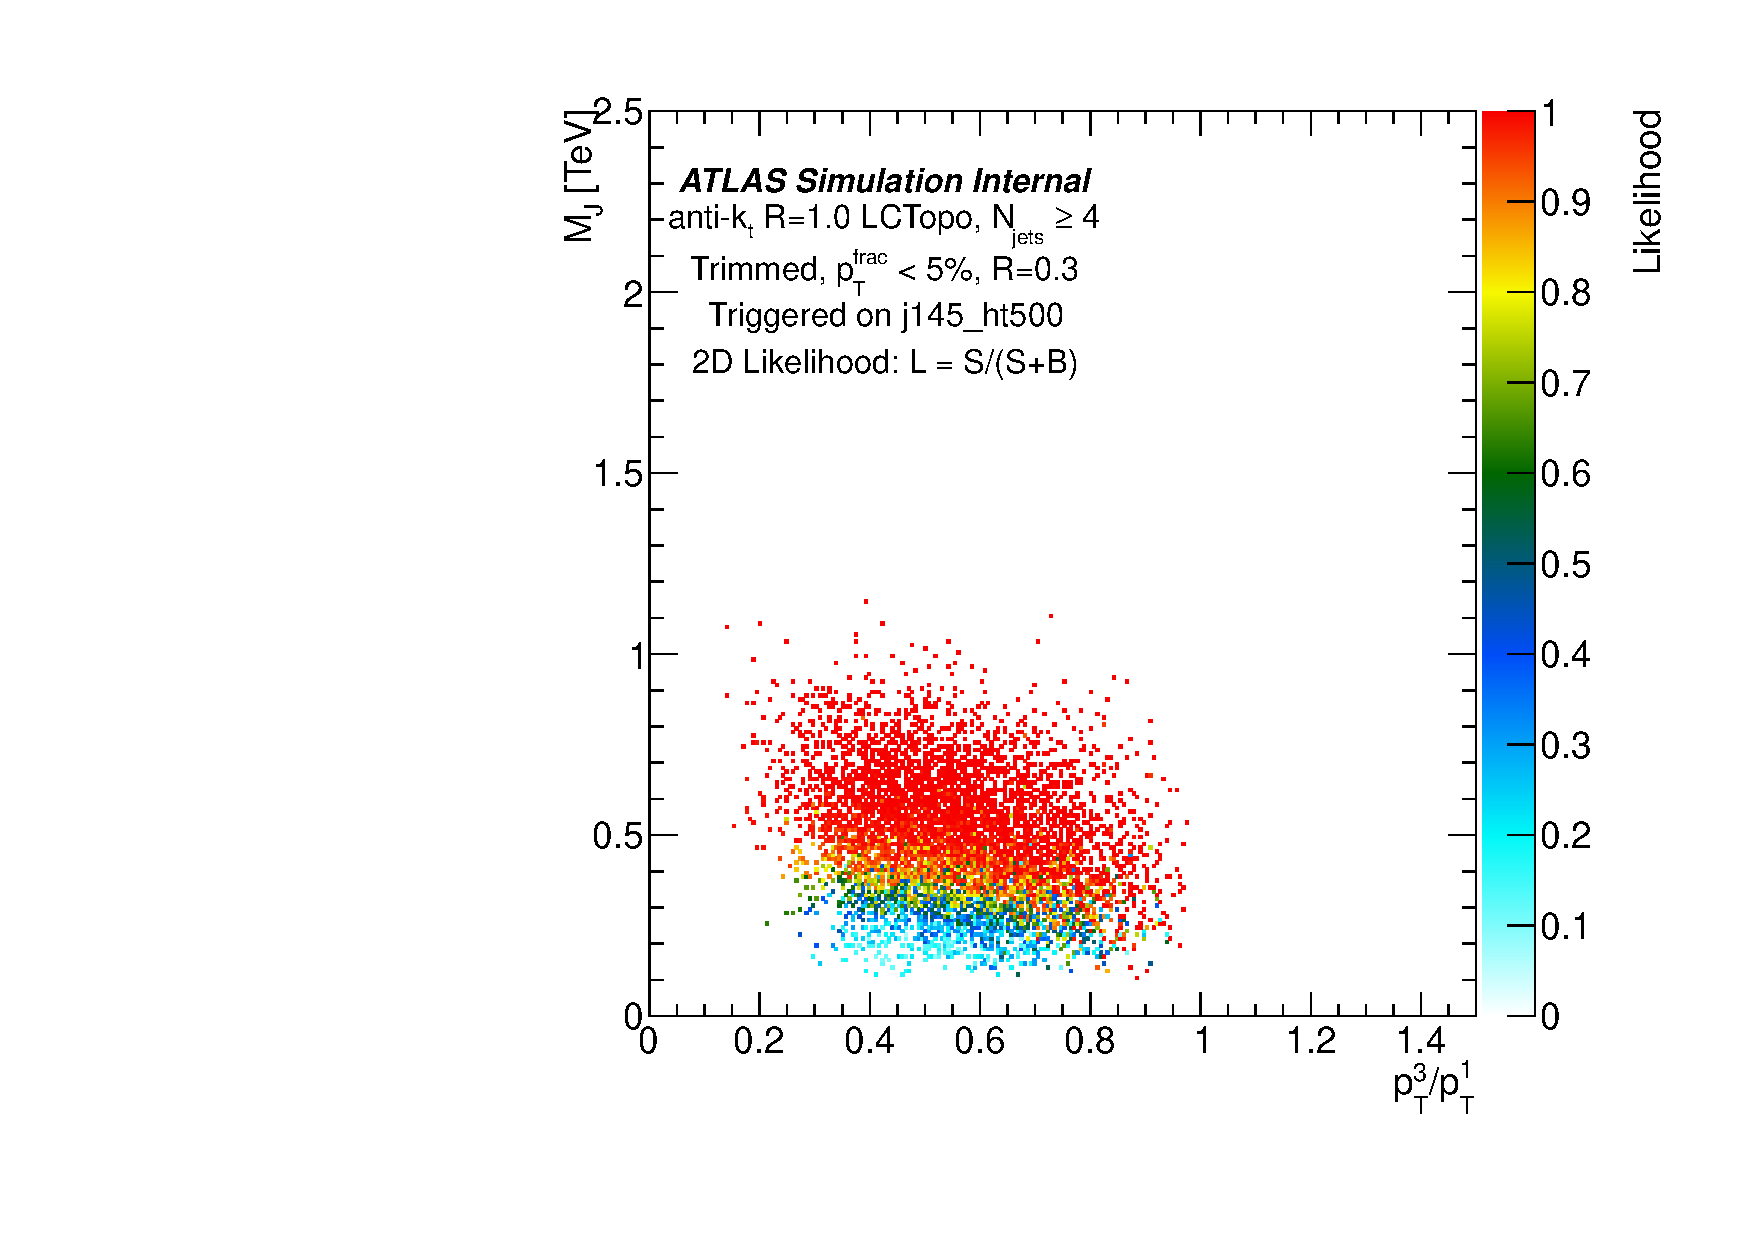
\includegraphics[width=0.5\textwidth]{INT/AntiKt10LCTopoTrimmedPtFrac5SmallR30_j145_ht500_NjetIncl_NFatJetMin4_MJ4_vs_PT31_SigPoint3_L_RPVGluino.pdf}
\label{fig:search:search:optimization:2D:PT31}
\caption{A likelihood for discrimination between a high $m_{\gluino}$ point and a \herwigpp di-jet background, using \MJ and $\pt^3/\pt^1$ as inputs.}
\end{figure}

%%%%%%%%%%%%%%%%  

Finally, Figure~\ref{fig:search:search:optimization:2D:DETA} shows the likelihood constructed with \Deta. Once again, the discrimination is improved by a diagonal cut, and even better, the correlation is significantly lower in these variables, at $<10\%$. Figure~\ref{fig:search:search:optimization:2D:DETAraw} shows the distribution in the \herwigpp di-jet sample: this evident very low level of correlation between the variables makes \Deta ideal to define signal and control regions, as will be discussed in Section~\ref{chapter:search:search:regions}. For this reason, the two variables used to define the analysis were chosen to be \MJ and \Deta.

%%%%%%%%%%%%%%%%

\begin{figure}
\centering
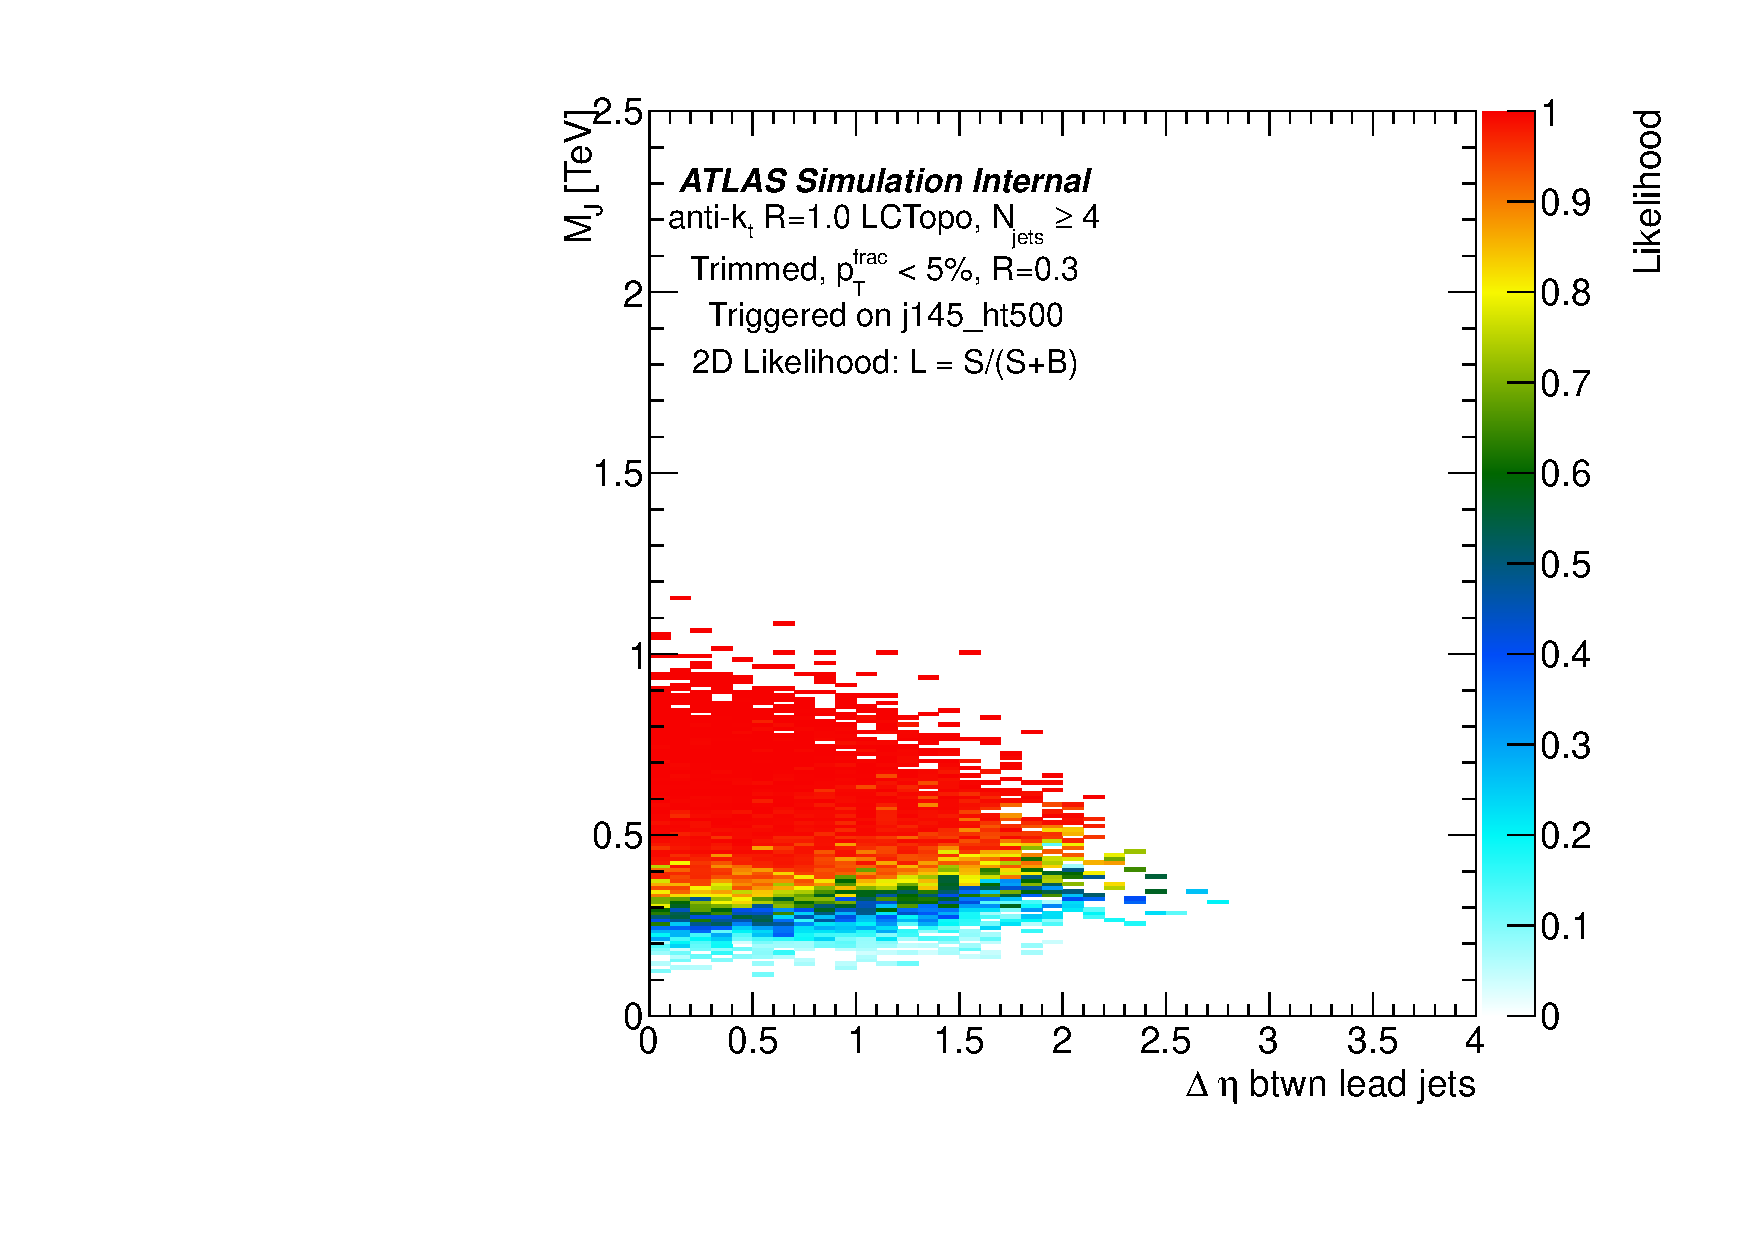
\includegraphics[width=0.5\textwidth]{INT/AntiKt10LCTopoTrimmedPtFrac5SmallR30_j145_ht500_NjetIncl_NFatJetMin4_MJ4_vs_DEta_SigPoint5_L_RPVGluino.pdf}
\label{fig:search:search:optimization:2D:DETA}
\caption{A likelihood for discrimination between a high $m_{\gluino}$ point and a \herwigpp di-jet background, using \MJ and $\Delta \eta$ as inputs.}
\end{figure}

%%%%%%%%%%%%%%%% 

%%%%%%%%%%%%%%%%

\begin{figure}
\centering
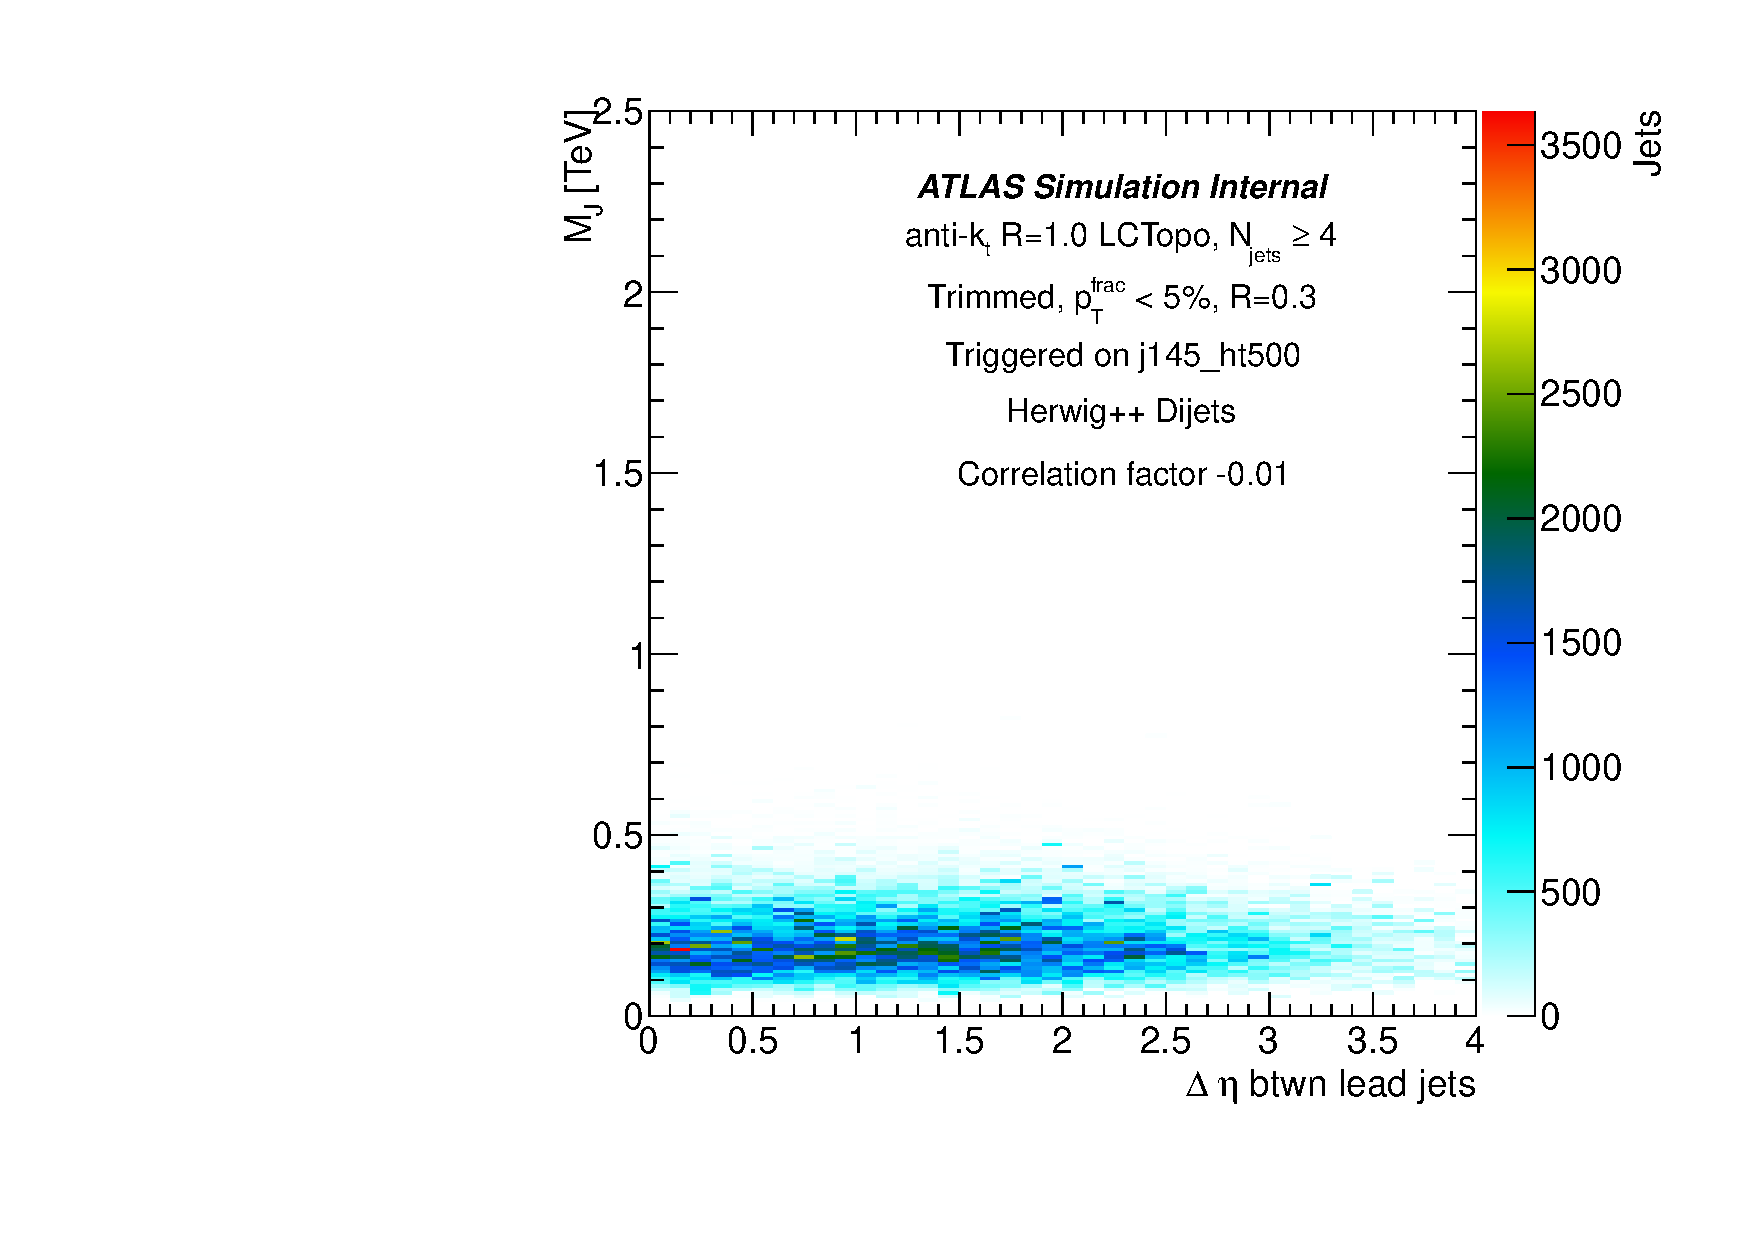
\includegraphics[width=0.5\textwidth]{INT/AntiKt10LCTopoTrimmedPtFrac5SmallR30_j145_ht500_NjetIncl_NFatJetMin4_MJ4_vs_DEta_SigPoint_RPVGluino.pdf}
\label{fig:search:search:optimization:2D:DETAraw}
\caption{A likelihood for discrimination between a high $m_{\gluino}$ point and a \herwigpp di-jet background, using \MJ and $\Delta \eta$ as inputs.}
\end{figure}

%%%%%%%%%%%%%%%% 


Note also that other combinations without \MJ were also considered: \Ht and $T_{32}$, for example, are substantially less correlated because \Ht does not use substructure information. These pairings were all less effective than \MJ and \Deta combination. Additionally, pre-selection cuts on $T_{32}$ and $T_{21}$ were attempted, in combination with the \MJ and \Deta variables: adding the additional discrimination from the n-subjettiness variables did not significantly increase the discrimination.


\subsection{Event and Trigger Selections}

To perform the analysis in data, only events which pass a general quality selection and particular trigger configuration are used. The quality selection is rather generic to many ATLAS analyses:
%
\begin{enumerate}
\item Events are required to have not occurred during periods with limited detector operations.
\item Events are required to contain a primary vertex consistent with the LHC beamspot, reconstructed from at least 2 tracks with transverse momenta $\pt^{\mathrm{track}} > 400$~MeV
\item Jets reconstructed with the anti-kt algorithm using a size parameter of $R = 0.4$ and a measured $\pt^{\mathrm{jet}}$ > 25 GeV are required to satisfy the “looser” requirements, which are targetted at reducing background from photons and electrons (by requiring the EM fraction to be at least 5\%), as well as poorly functioning regions of the detector (by requiring that no jet be allowed to have more than 99\% of its energy in one layer)~\cite{jetquality}. Furthermore, jets with a majority of their energy in the HEC are required to have no problematic noise characteristics, and no more than 60 GeV of negative energy (both indications of read-out problems); jets enclosed in the ECal are required to have good pulse shapes in all layers. If any jet with $\pt^{\mathrm{jet}} > 25$~GeV is found to fail any of these criteria, the event is rejected.
\end{enumerate} 
%

A three-stage trigger system is used to select interesting events for the analysis. The Level-1 trigger... \editnote{Need to add L1 and L2 details!}


The high-\pt trigger at the event filter, \texttt{EF\_j360\_a10tcem}, has an online cut of $360$~GeV on the leading jet \pt, constructed using the \antikt $R=1.0$ algorithm from online EM-scale topo-clusters. Fluctuations due to jet energy resolution and differences between online and offline reconstruction (for example, the online jet has no trimming applied, and the clusters are only EM-scale instead of locally calibrated) mean that a jet with a given offline \pt may or may not have actually fired the trigger. As the modeling of the trigger in the simulation is somewhat unrelaible, we require the offline jet \pt to be fully efficient: i.e., that the \pt is so high that the trigger is guaranteed to have fired.

To measure the efficiency of the \texttt{j360} trigger, its measurements are compared to a \textit{reference} trigger. A reference trigger has a lower \pt threshold, but is pre-scaled to avoid taking data at too high a rate. A higher \pt threshold trigger is considered fully efficient if it fired on every event on which the lower \pt treshold trigger fired. The ratio of their efficiencies is called the \textit{turn-on} curve. In order to make the trigger fully efficient an offline \pt cut on the trimmed jet pT at $500$~GeV was used, as motivated by Figure~\ref{fig:search:search:trig:pt1}. 

%% pT1 and cum eff
\begin{figure}[!ht]
  \centering
  \subfigure[Leading $\ptjet$]{
    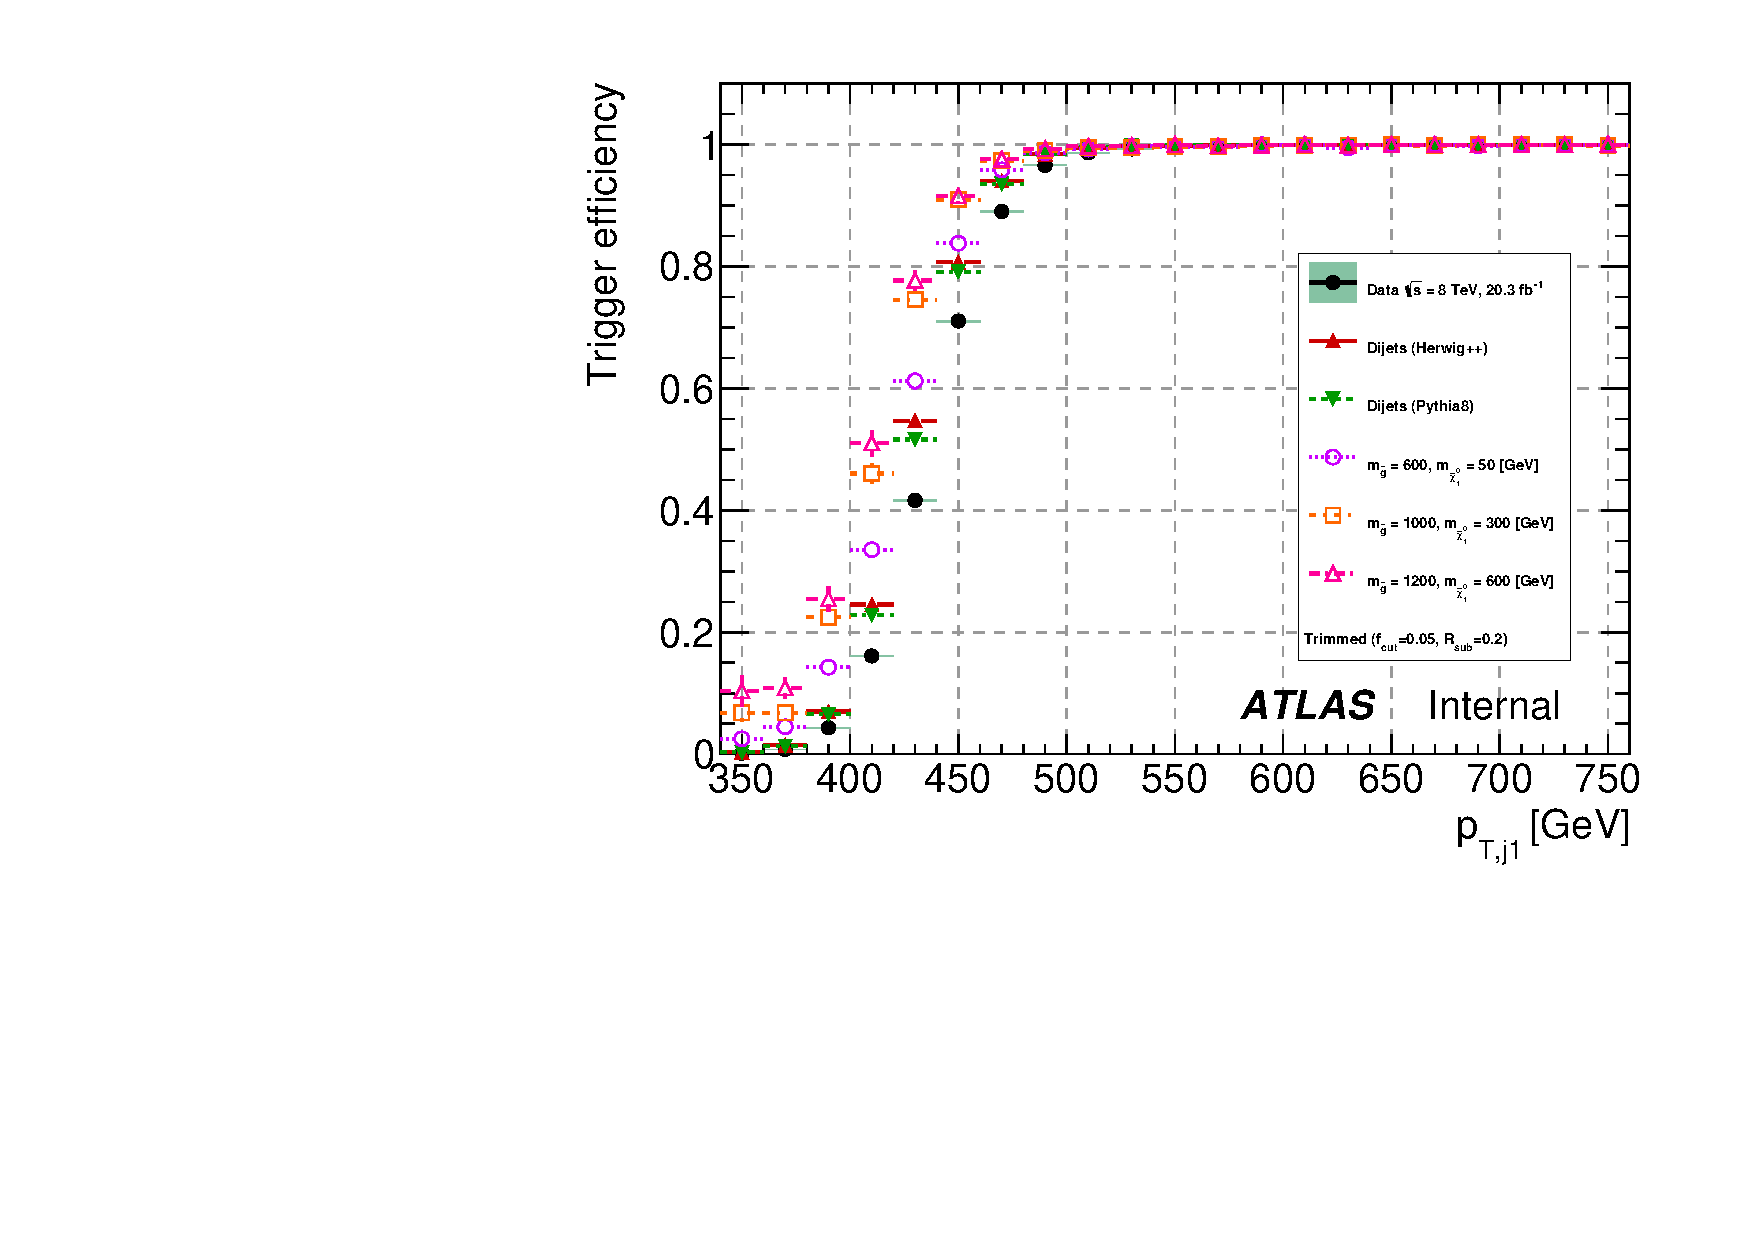
\includegraphics[width=0.48\columnwidth]{INT/Trigger/overlay_Eff_jet_pT1_Trig_10q_Incl_AntiKt10LCTopoTrimmedPtFrac5SmallR30.pdf}
    \label{fig:search:search:trig:pt1:eff}}
  \subfigure[Cumulative efficiency (leading $\ptjet>500$~GeV)]{
    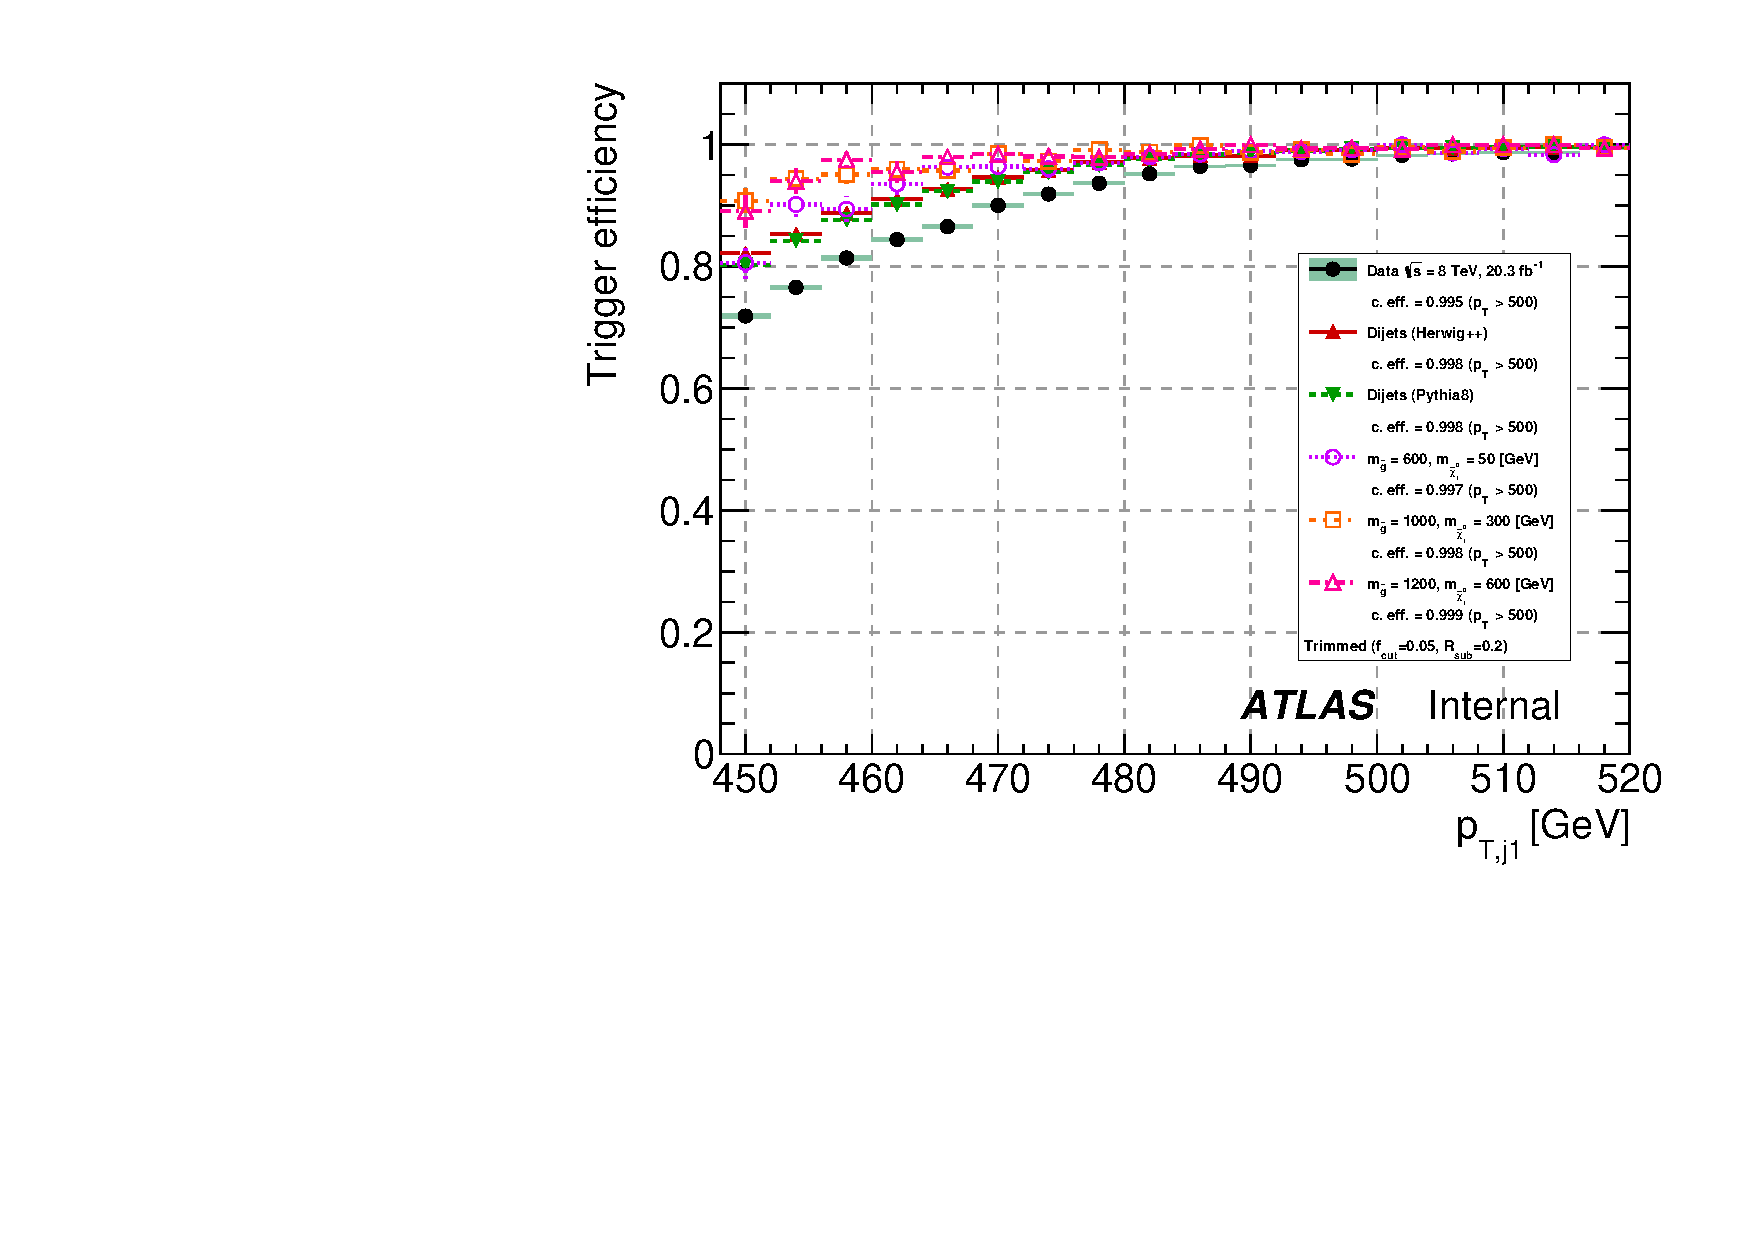
\includegraphics[width=0.48\columnwidth]{INT/Trigger/overlay_Eff_ZoomDetailed_CumEff500_jet_pT1_Trig_10q_Incl_AntiKt10LCTopoTrimmedPtFrac5SmallR30.pdf}
    \label{fig:search:search:trig:pt1:cumeff}}
    \caption{Efficiency for the \texttt{EF\_j360\_a10tcem} trigger as a function of leading $\ptjet$. The efficiency is calculated using \texttt{EF\_j240\_a10tcem} as the reference trigger. The cumulative efficiency (shown in the legend) is the ratio of the sum of the number of events passing the trigger \texttt{EF\_j360\_a10tcem} and the number of events passing the reference trigger \texttt{EF\_j240\_a10tcem}. }
  \label{fig:search:search:trig:pt1}
\end{figure}
%%------------------------------

The \texttt{j360} trigger is fully unprescaled, and the integrated luminosity collected by the trigger (and passing basic detector quality criteria) corresponds to the full 20.3 \ifb ATLAS dataset.

\subsection{Analysis Regions}
\label{chapter:search:search:regions}

Several basic requirements in the analysis have thus been defined: we require high quality events, we use events with several \largeR jets, and we require the leading such jet to have \ptjet > 500 GeV. Two classes of region are now defined: the exclusive 3-jet control region (referred to as the 3jCR) and the various $\geq 4$ jet regions (referred to with the prefix 4j). These are summarized in Figure~\ref{fig:search:search:regions}. To count for the signal region definition, as previously discussed, a jet must have $\pt > 100$~GeV and $|\eta| < 2.5$. 

The 3jCR is inclusive in all variables. This region is strongly enriched in the multi-jet background: a requirement of exactly 3-jets highly reduces the signal in this region (and moreover, the natural cross-section of a 3-jet region is an order of magnitude higher than that of the $\geq 4$ jet region). This makes the 3jCR a perfect candidate for the training sample of the substructure template background estimation technique.

As previously implied in \ref{chapter:search:search:optimization}, $\Deta$'s power is not very strong, but it is rather uncorrelated with \MJ. This means that a selection on $\Deta$ designed to select background-- i.e., a cut on $|\Deta|$ to be high-- can expose a region with high \MJ, but comparatively low expected signal. This allows for the assessment of the templates and the derivation of additional topology related uncertainties, even in the 4j regions. The 4jCR (control region) is defined with $\Deta > 1.4$; the 4jVR (validation region) is defined as $1.4 >\Deta > 1.0$. The two separate regions allow for the derivation of corrections and uncertainties in one, and then the assessment of these in an orthogonal region. Finally, a cut of $|\Deta| < 0.7$ defines the signal region (4jSR), where new physics is hoped to be found.

%%------------------------------
\begin{figure}[!ht]
  \centering
  \subfigure[3jCR]{
    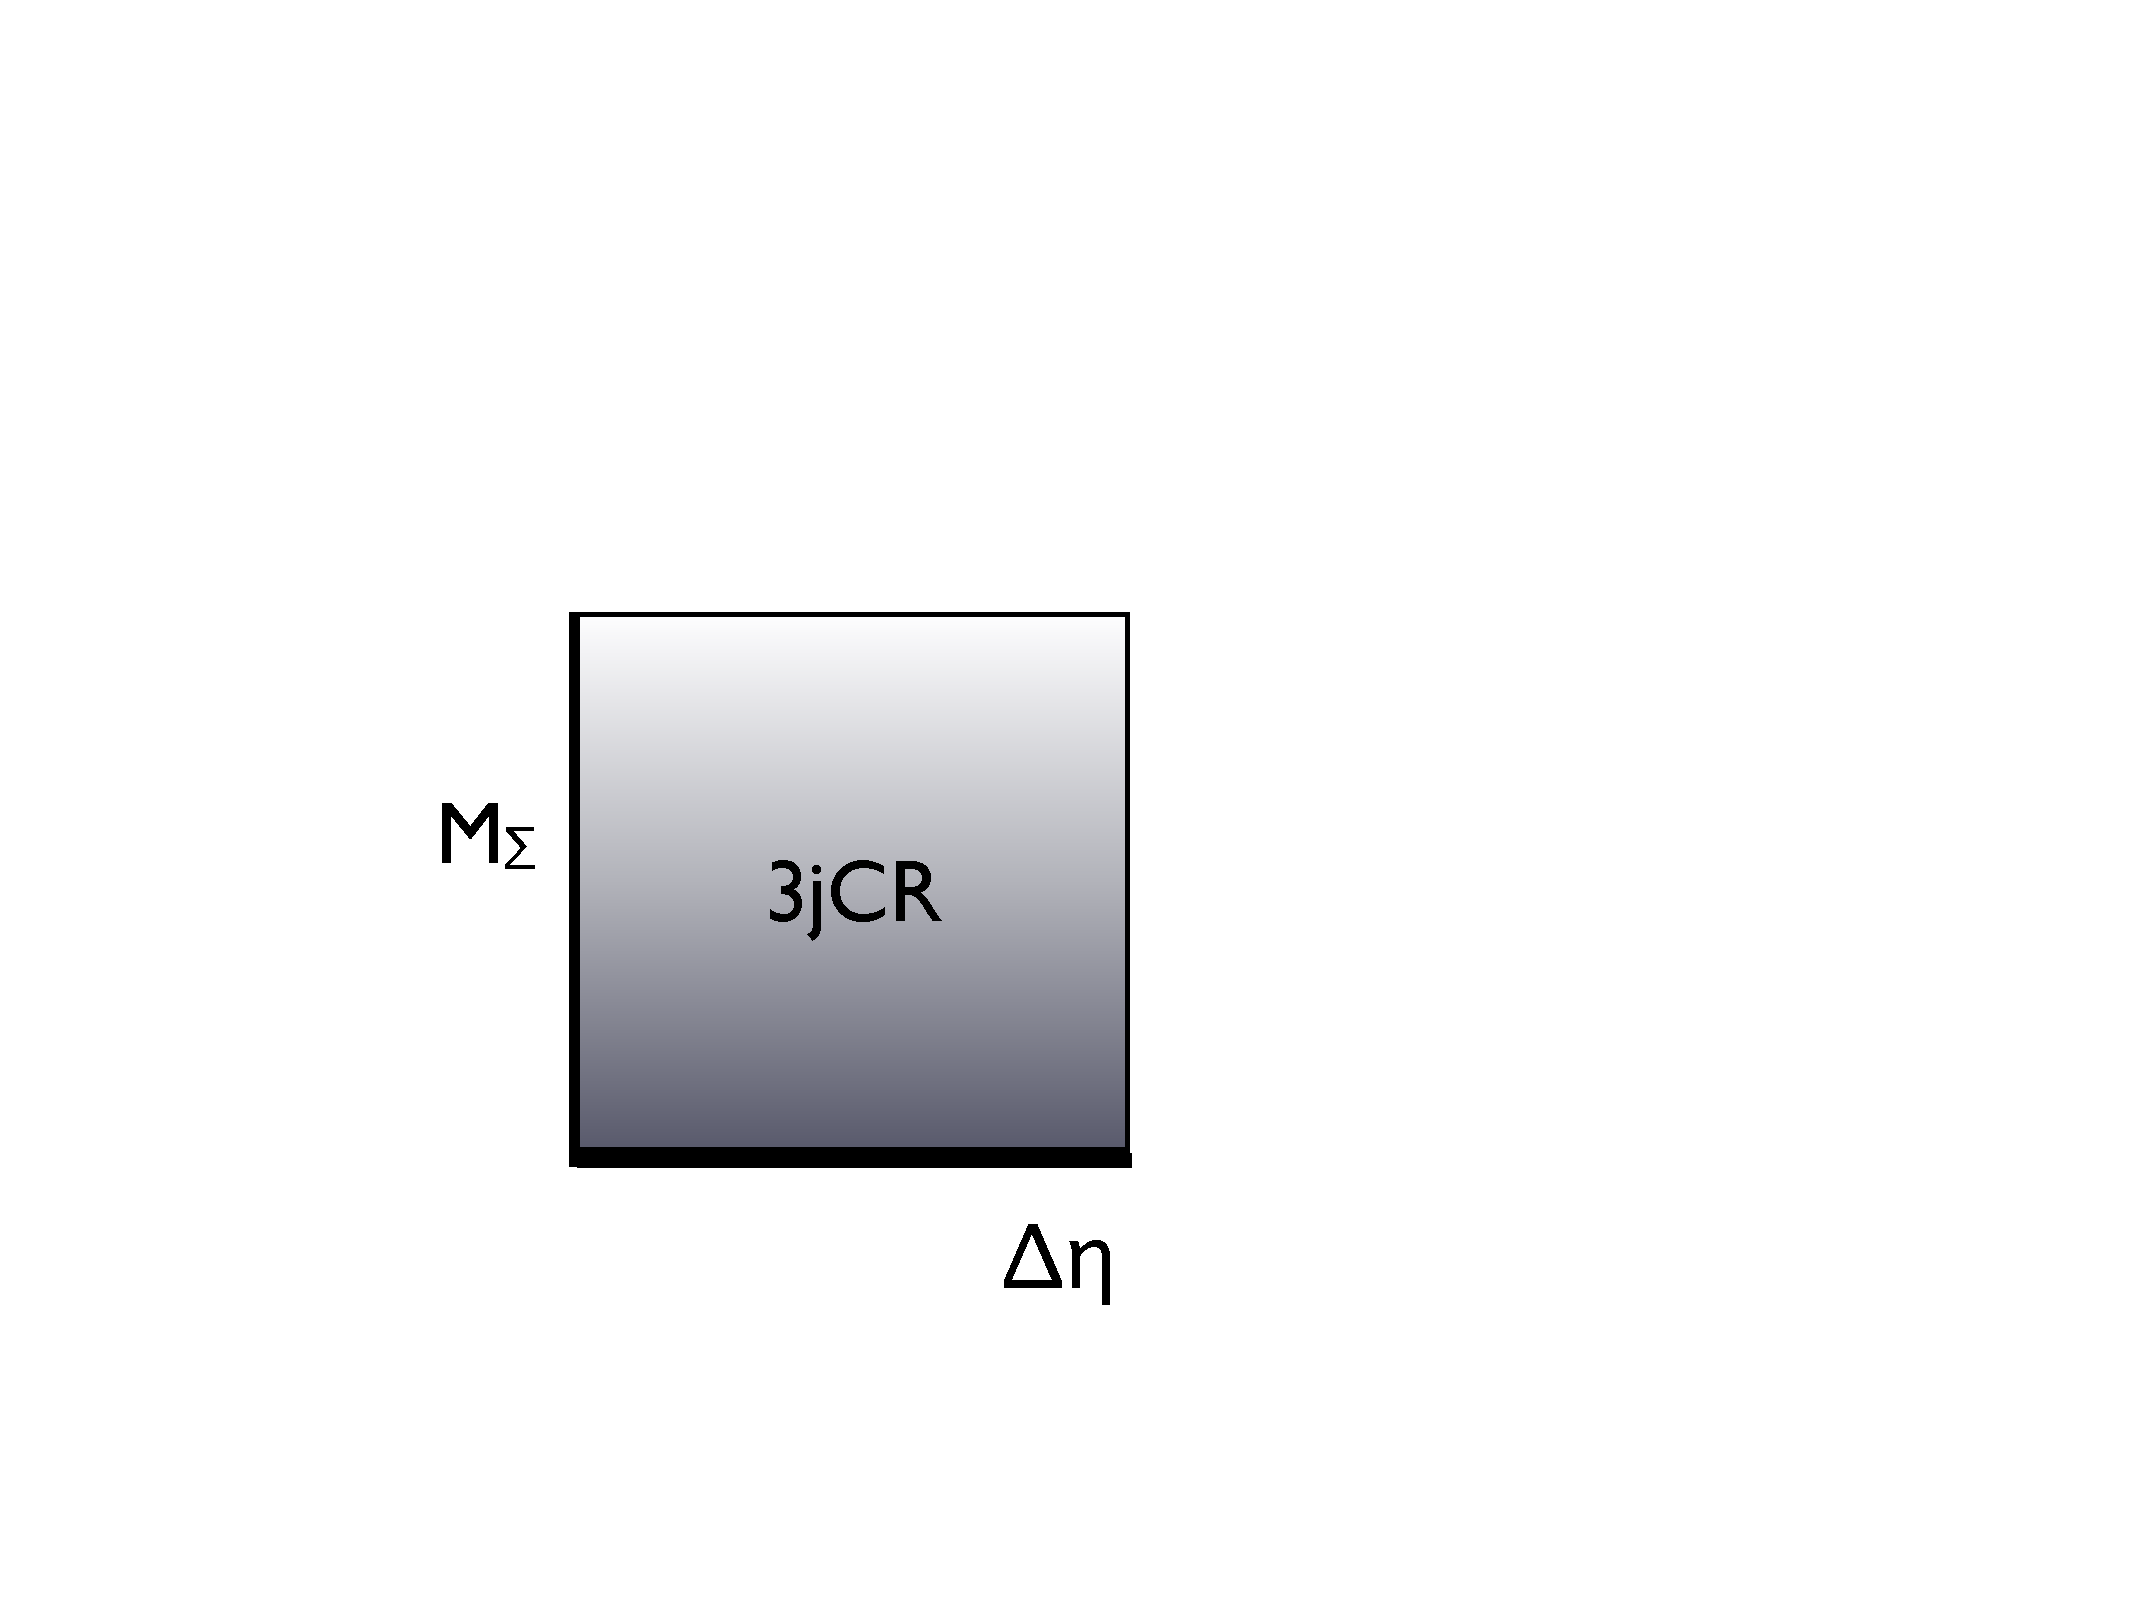
\includegraphics[width=0.48\columnwidth]{INT/3jetsketch}
    \label{fig:search:search:regions:3j}}
  \subfigure[4j regions]{
    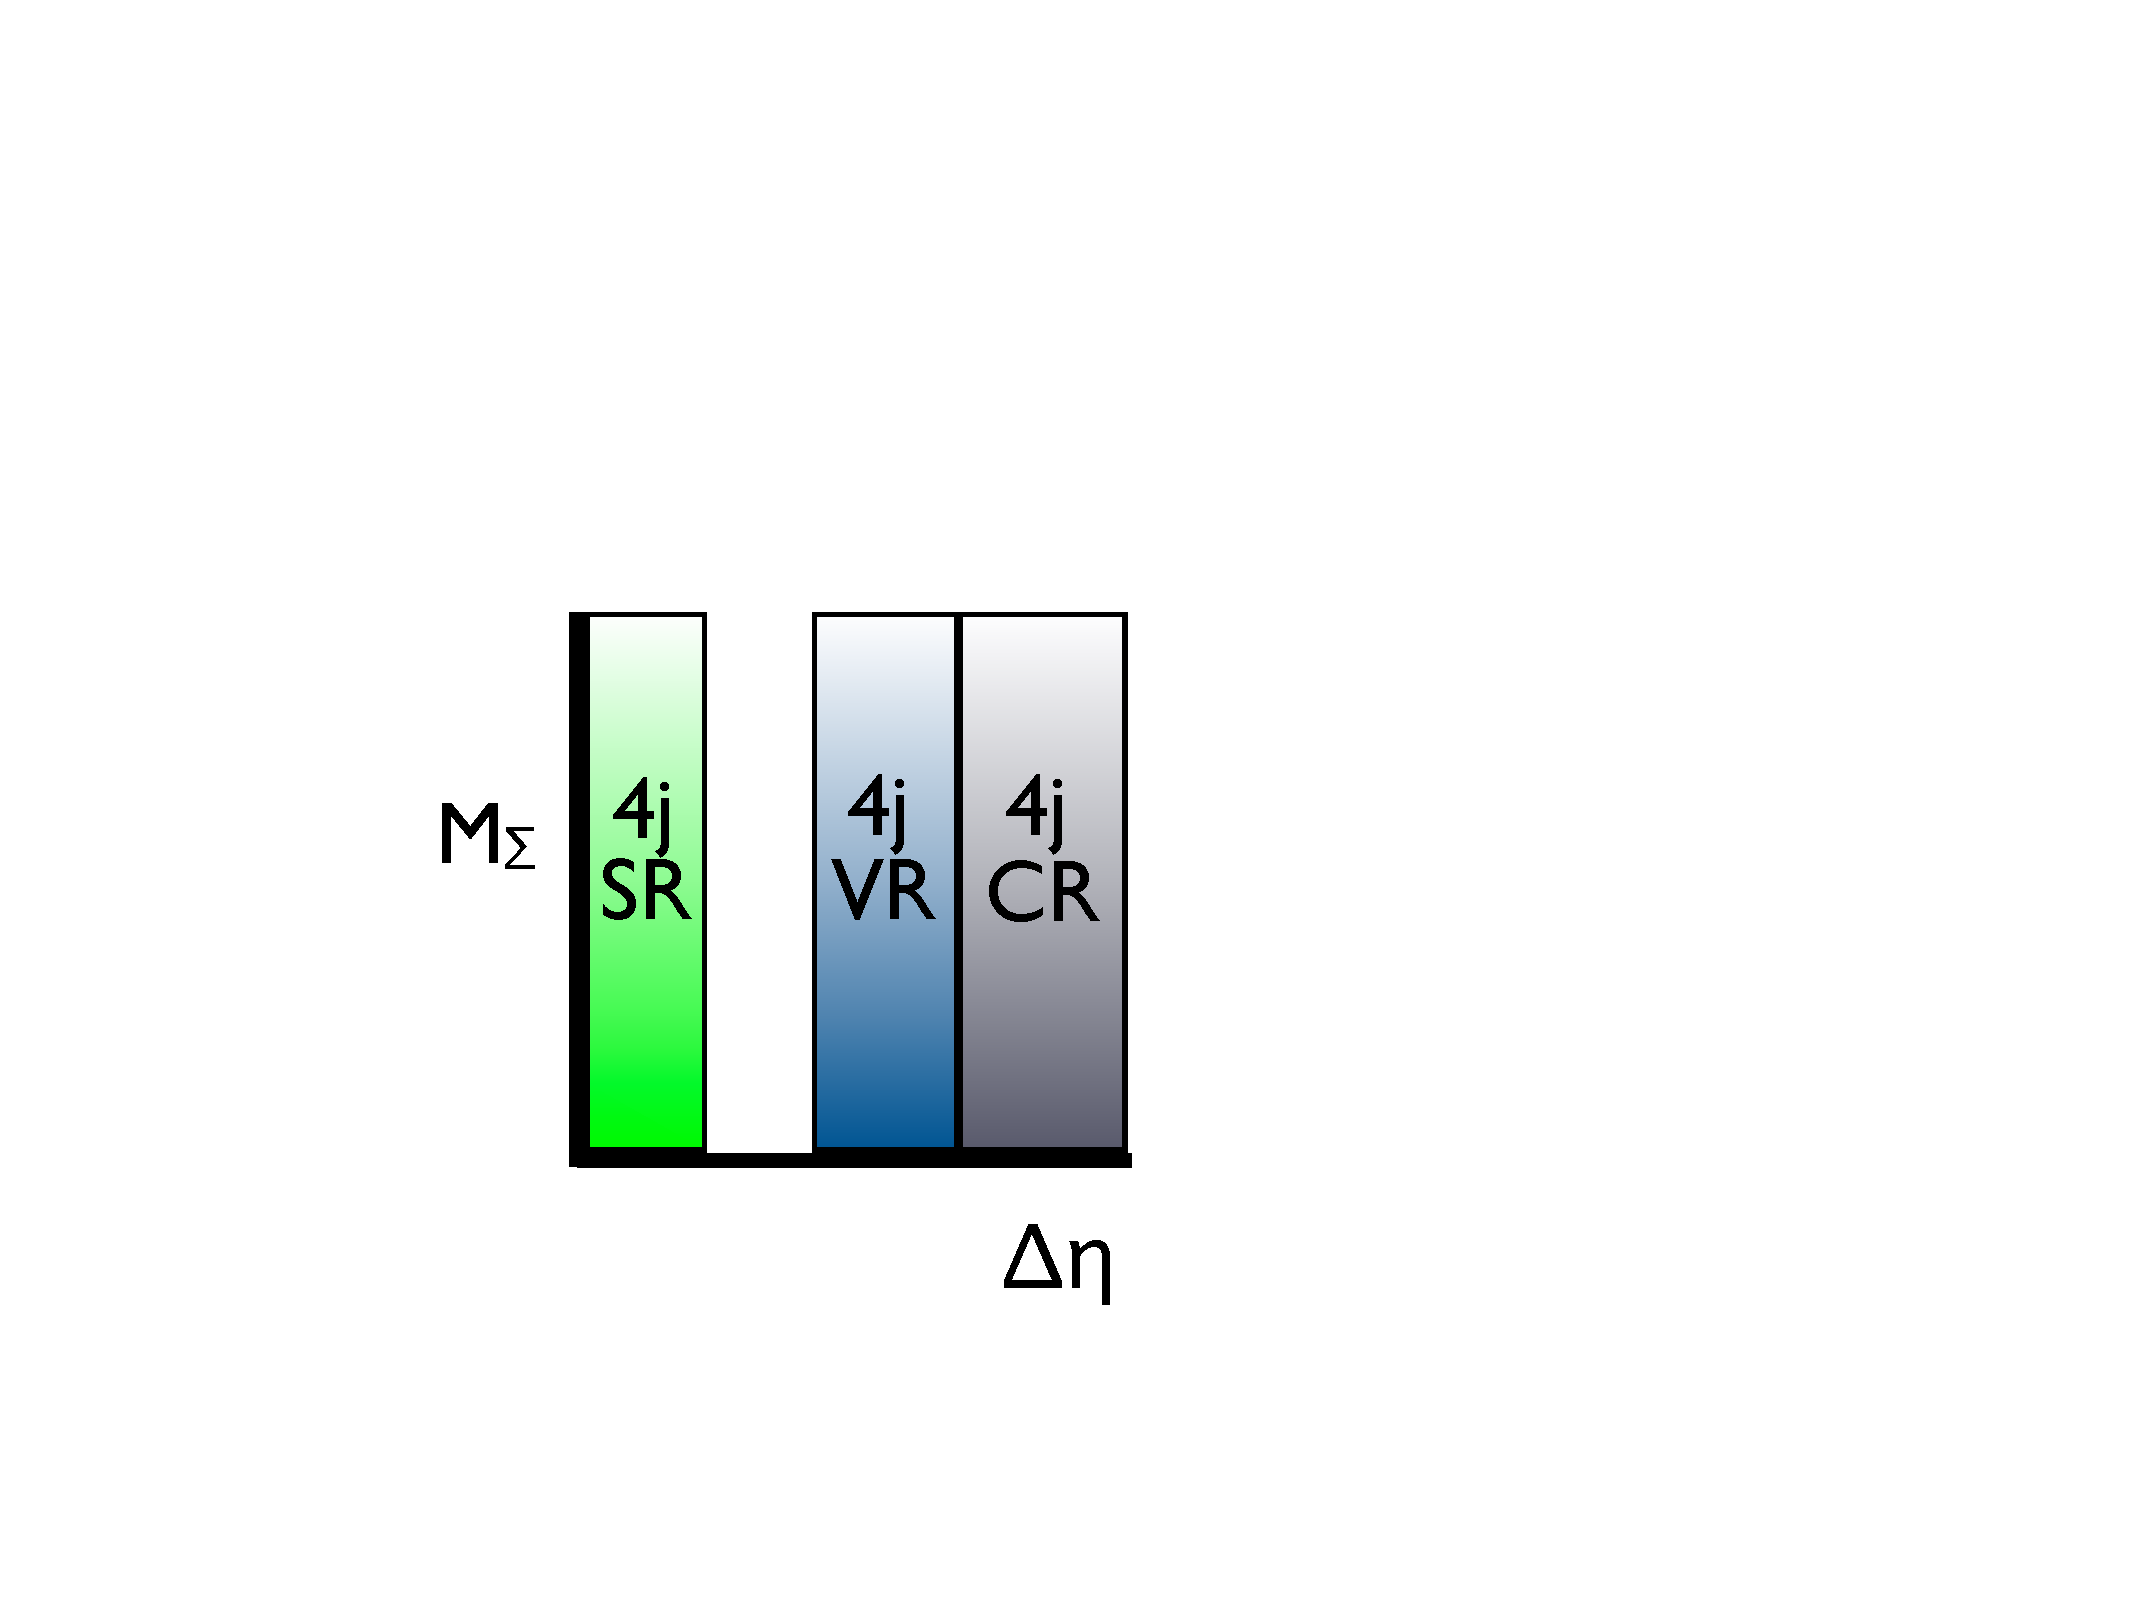
\includegraphics[width=0.48\columnwidth]{INT/4jetsketch.pdf}
    \label{fig:search:search:regions:4j}}
    \caption{Diagrams summarizing the 3j and 4j regions used in the analysis}
  \label{fig:search:search:regions}
\end{figure}
%%------------------------------

One additional criteria is based on the strength of the $\pt^3/\pt^1$ variable previously discussed. Two different 4jSR's are defined to take advantage of the relative power of $\pt^3$ in various portions of the \gluino-\lsp mass plane. The SR100 is defined with the nominal $\pt^3$ threshold of $100$ GeV, and the SR250 is defined with $\pt^3 > 250$~GeV. $\pt^3/\pt^1$ is not used, as it is more straightforward to apply the cut to the \pt of the third jet only. 

As will be described later, the \MJ \textit{distribution} in the SR100 and SR250 is tested for its compatibility to the SM prediction: the template is method is able to predict a full shape, not just a value after a cut, and so the analysis takes full advantage of this additional information. In order to facilitate more straightforward comparisons to theoretical results, one additional region, defined similarly to SR250 but using a strict cut of $\MJ > 625$~GeV (SR1), is used. 

All of the various regions of the analysis are summarized in Table~\ref{tab:search:search:regions:CRselections}. Each sub-region of the 4jSR has a corresponding 4jVR and 4jCR; the 3jCR is used to train these all together. Since the only differences between the various 4j regions are cuts on \pt and $\eta$, which are controlled for by the template, this uniform training is possible.

%%------------------------------
  \begin{table}[!htb]
    \begin{center}
	  \begin{tabular}{r|c|c|c|c|c}
	    \hline \hline
Region  &   \Njet       & $\Deta$    & \ptthr & \ptfour & \MJ \\ 
Name  &         &     & [GeV] & [GeV] & [GeV]\\ \hline   
 		 3jCR  & $\Njet=3$     & --         &              & --            & -- \\ \hline
		 \multirow{2}{*}{4jCR}  & \multirow{2}{*}{$\Njet\geq4$}  & \multirow{2}{*}{$>1.40$}    & $>100$       & \multirow{2}{*}{$>100$}        & -- \\
		 	   &               &            & $>250$       &               & -- \\ \hline
		 \multirow{2}{*}{4jVR}  & \multirow{2}{*}{$\Njet\geq4$}  & \multirow{2}{*}{1.0--1.40} & $>100$       & \multirow{2}{*}{$>100$}        & -- \\
		 	   &               &            & $>250$       &               & -- \\ \hline
		 SR1   &               &            & $>250$       &               & $>625$ \\
		 SR100 & $\Njet\geq4$  & $<0.7$     & $>100$       & $>100$        & $>350$ (binned) \\
		 SR250 &               &            & $>250$       &               & $>350$ (binned) \\
		\hline \hline
	  \end{tabular}
    \end{center}
  \caption{Control (CR), validation (VR), and signal regions (SR) used for the analysis. \ptthr and \ptfour represent the transverse momentum of the third and fourth jet in \pT, respectively.}
  \label{tab:search:search:regions:CRselections}
  \end{table}%      
%%------------------------------



	
	\subsection{Background Estimates}
	\label{chapter:search:search:background}

Now that the sensitive variables, background estimate strategy, and analysis regions are defined, it is time to actually develop the expected Standard Model contribution to the signal region. The first priority is assessing the construction of the templates in the 3jCR.

It should be noted that for the purposes of constructing the templates, steeply falling distributions like jet masses and \pt are actually not very optimal: the rapidly falling distribution means that statistics are not evenly distributed through the boundaries of the variable. The solution is to apply a transformation to these two variables: instead of \pt, $\log(\pt/50)$ is used, and instead of mass, $-\log(m/\pt)$ is used. These transformations are trivial to reverse back into \pt and $m$ after the background prediction is extracted.

\subsubsection{Template Construction in the 3jCR}

Should the templates for jets be constructed inclusively-- that is, without differentiating between jet number-- or exclusively? Figure~\ref{fig:search:search:background:3jCR} shows the results of two possibilities for the leading (left) and subleading (right) jets.  In this figure, the black points correspond to the actual mass distributions, the blue points correspond to the exclusively constructed template, and the red points correspond to an inclusively (in the leading two jets) constructed template. The inclusive template has an advantage of a doubling in the size of the training sample, but the performance in reproducing the input distribution is reduced. A slope exists in the ratio of the inclusive template to the actual mass points, and this goes in different directions for the leading and subleading jets: this indicates that the inclusive template is correctly averaging between the two distributions, but that there is in fact a difference between them (as was also observed in the equivalent theory studies~\cite{MassTemplates}).


%%------------------------------
\begin{figure}[!ht]
  \centering
  \subfigure[1st leading jet template]{
    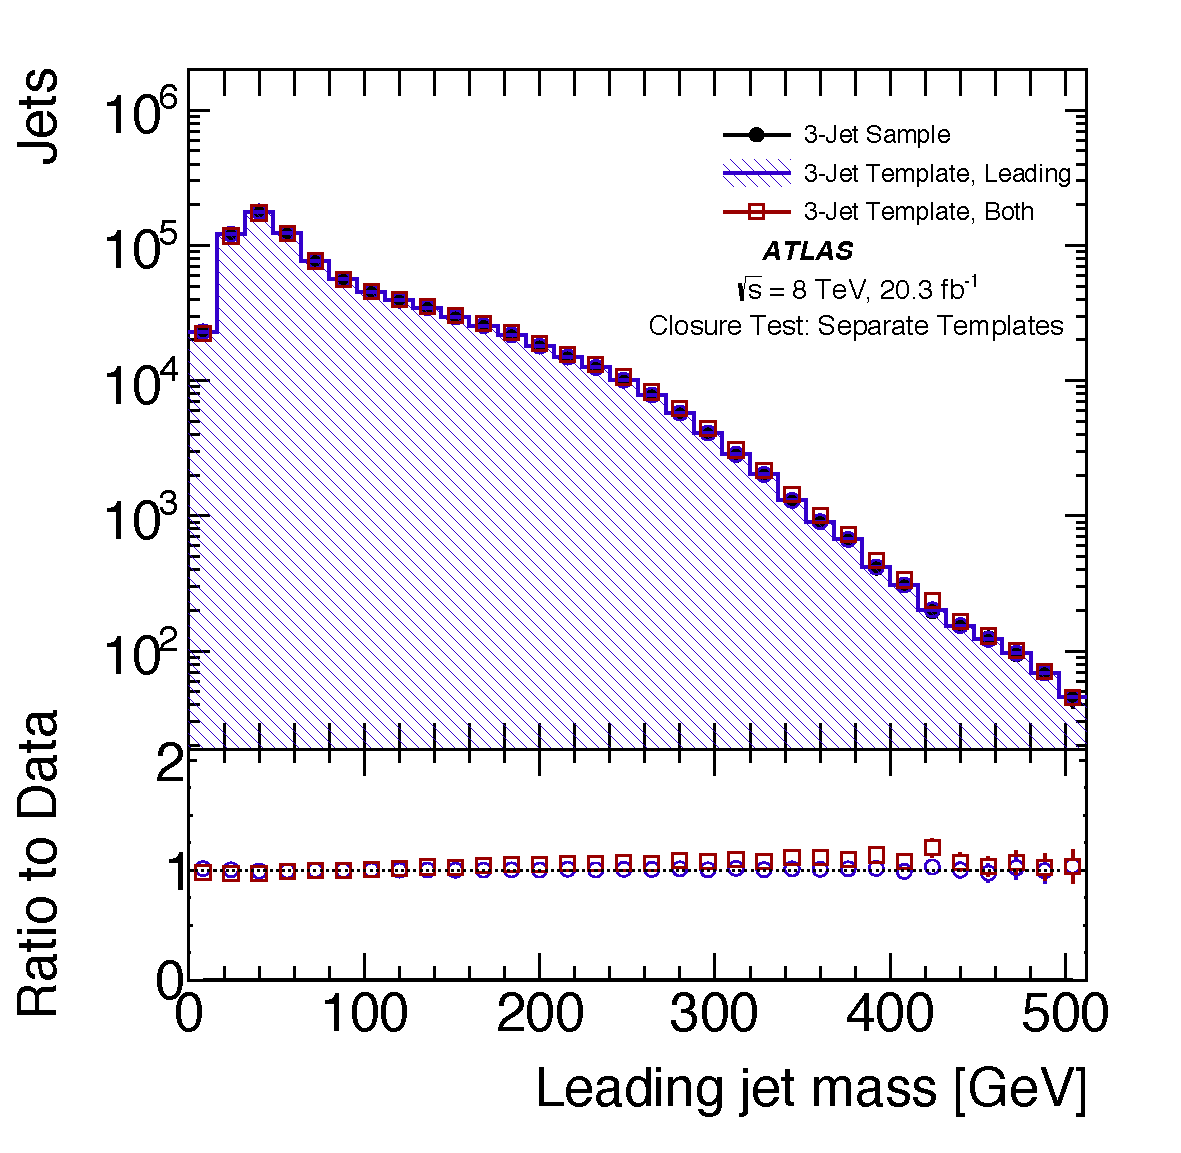
\includegraphics[width=0.48\columnwidth]{mj/figaux_14a.pdf}}
    % \label{fig:search:search:regions:3j}}
  \subfigure[2nd jet template]{
    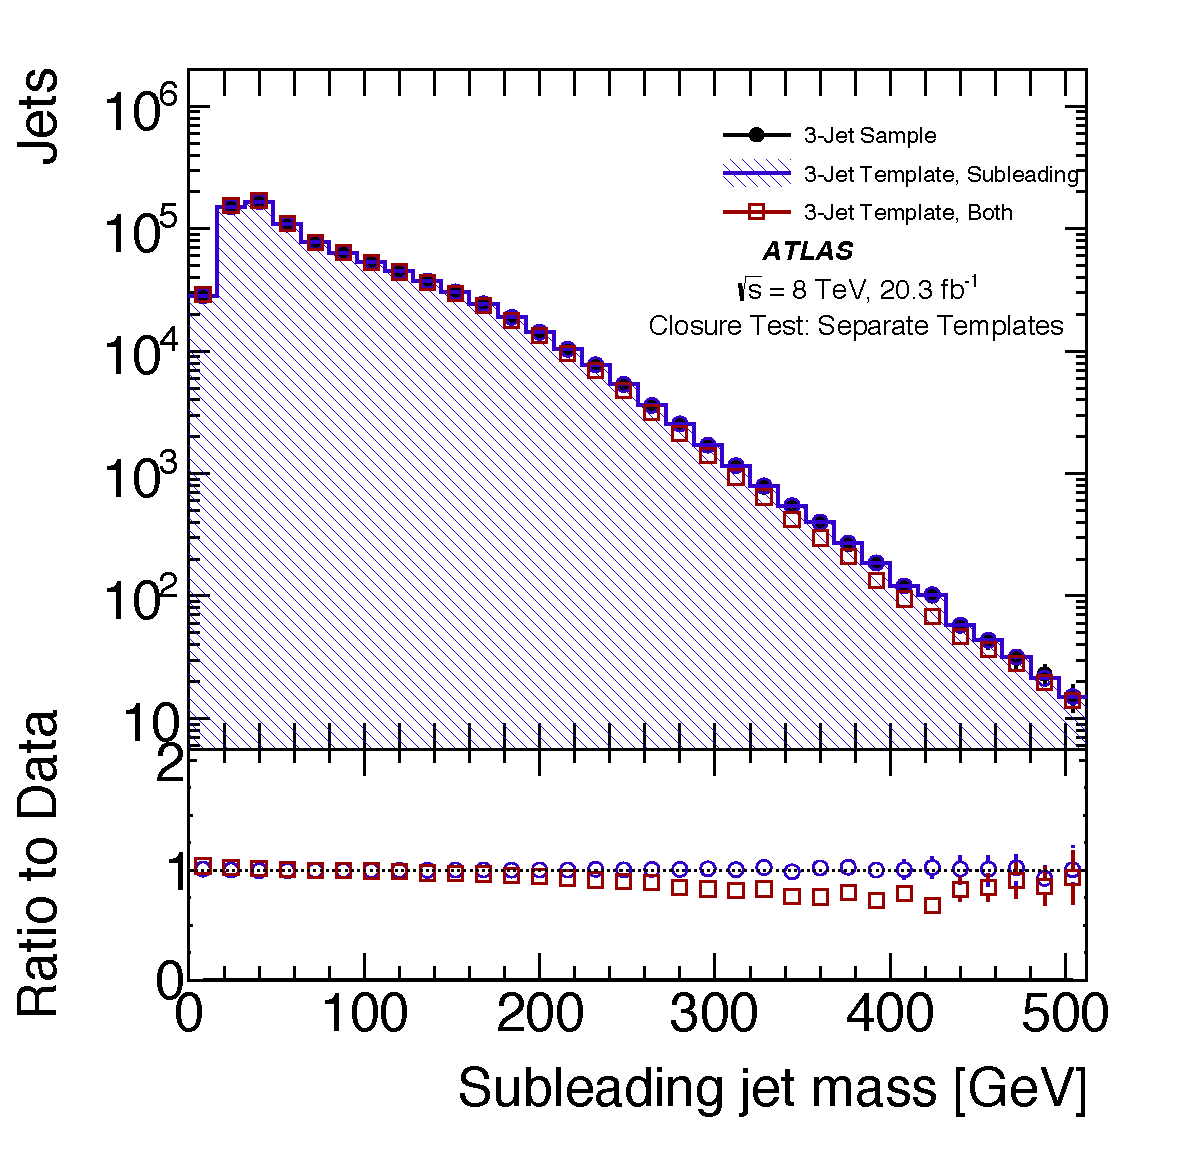
\includegraphics[width=0.48\columnwidth]{mj/figaux_14b.pdf}}
    % \label{fig:search:search:regions:4j}}
    \caption{Templates constructed with various inputs, compared to actual mass distributions of jets in the 3jCR, for the leading and subleading jets.}
  \label{fig:search:search:background:3jCR}
\end{figure}
%%------------------------------

Figure~\ref{fig:search:search:background:3jCRThird} shows a similar comparison for the third leading jet. The black points are again the distribution of actual jet masses in the 3jCR, while the blue are the outputs of a template constructed with only the third leading jet, and the red points are a template constructed from only the first two jets. This shows the marked difference between the first two jets and the third: while using a training of the leading on the subleading would have been quite close (double the difference observed in Figure~\ref{fig:search:search:background:3jCR}), the difference here is much larger. For this reason, the templates for all the jets are constructed inclusively. It is still an open question of how the fourth leading jet should be modelled; this will be discussed shortly.

%%%%%%%%%%%%%%%%

\begin{figure}
\centering
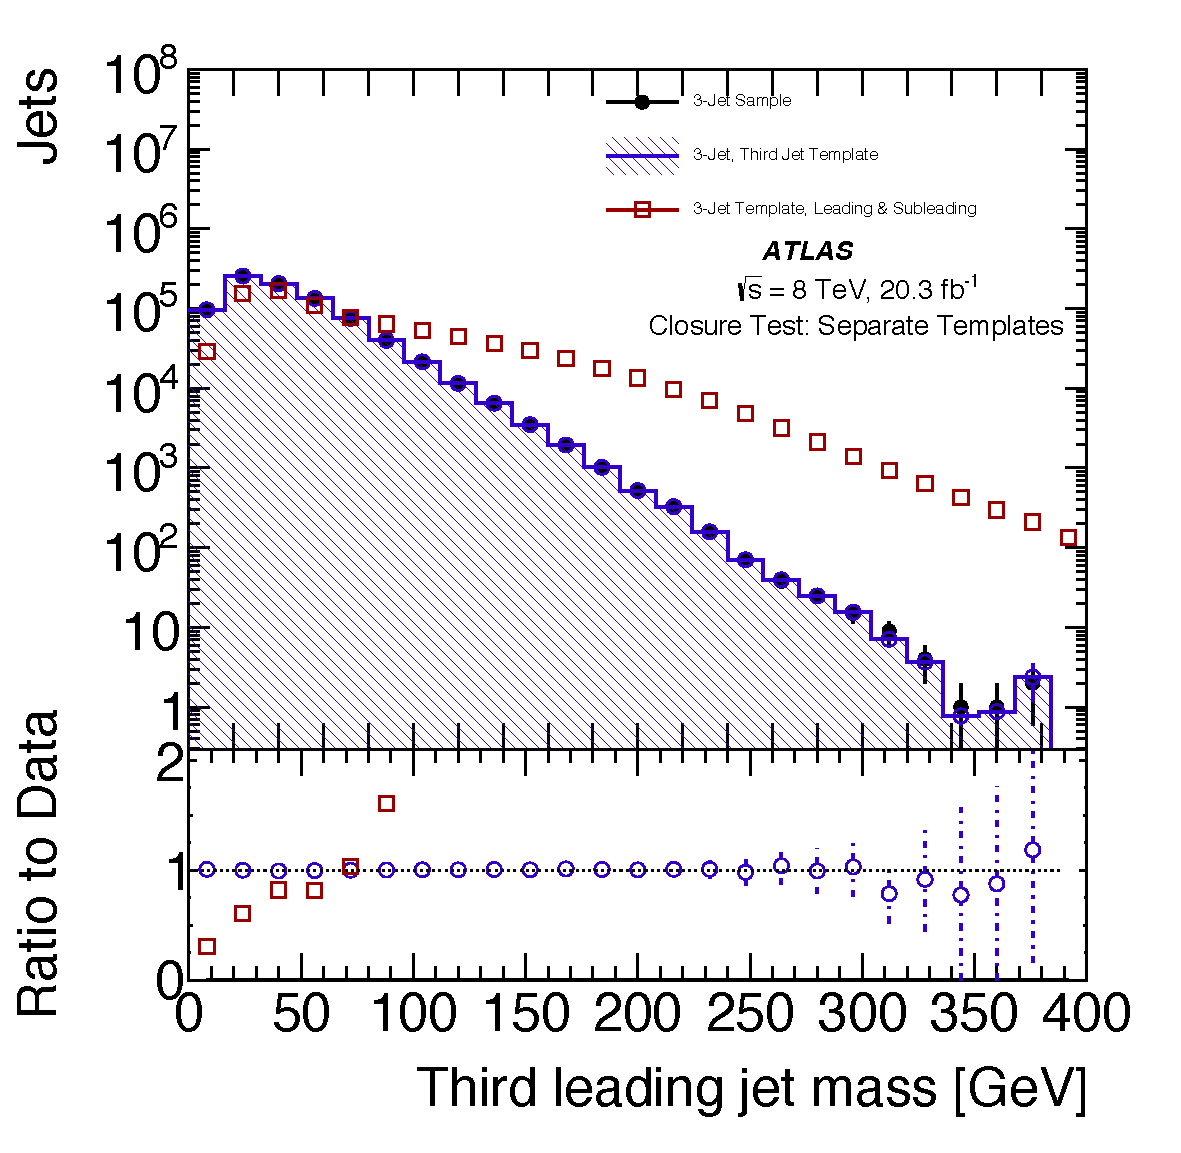
\includegraphics[width=0.5\textwidth]{mj/figaux_14c.pdf}
\label{fig:search:search:background:3jCRThird}
\caption{Templates constructed with various inputs, compared to actual mass distributions of jets in the 3jCR, for the third leading jet.}
\end{figure}

%%%%%%%%%%%%%%%% 

Next is the consideration of input variables to the templates: in particular, since the $\Deta$ cuts in the 4j region will shape the $\eta$ distributions used as inputs to the templates, it is important to consider whether there is any dependence on the mass from the jet $\eta$. In principle, the calibration of the mass has eliminated any detector-related component to this dependence, but there can be effects due to jet physics.


Figure~\ref{fig:search:search:background:closure:eta} presents the result of the study of the dependence of the jet templates on the jet $\eta$. In this study, the templates are derived either without (dark blue) or with (light purple) an explicit dependence on the jet $\eta$. Three different kinematic samples are then used to test the closure of the method: Figure~\ref{fig:search:search:background:closure:inclusive} uses an inclusive 3-jet kinematic sample, Figure~\ref{fig:search:search:background:closure:higheta} uses a high $\eta$ ($|\eta|>1.8$) kinematic sample, and Figure~\ref{fig:search:search:background:closure:loweta} uses a low $\eta$ ($|\eta|<0.7$) kinematic sample. In the latter two cases, the template formed with an explicit dependence on $\eta$ is observed to perform significantly better than the the inclusive template. An $\eta$-dependent template is therefore adopted as the approach to be used in deriving the template for the full \MJ distribution. Note that 10 bins in $|\eta|$ are used, leading to, in the worst case, a degradation in statistical power of about a factor of 3 in the central $\eta$ bins.

%%------------------------------    
\begin{figure}[!ht]
  \centering
  
  \subfigure[Leading jet mass and template (inclusive in $\eta$)]{
    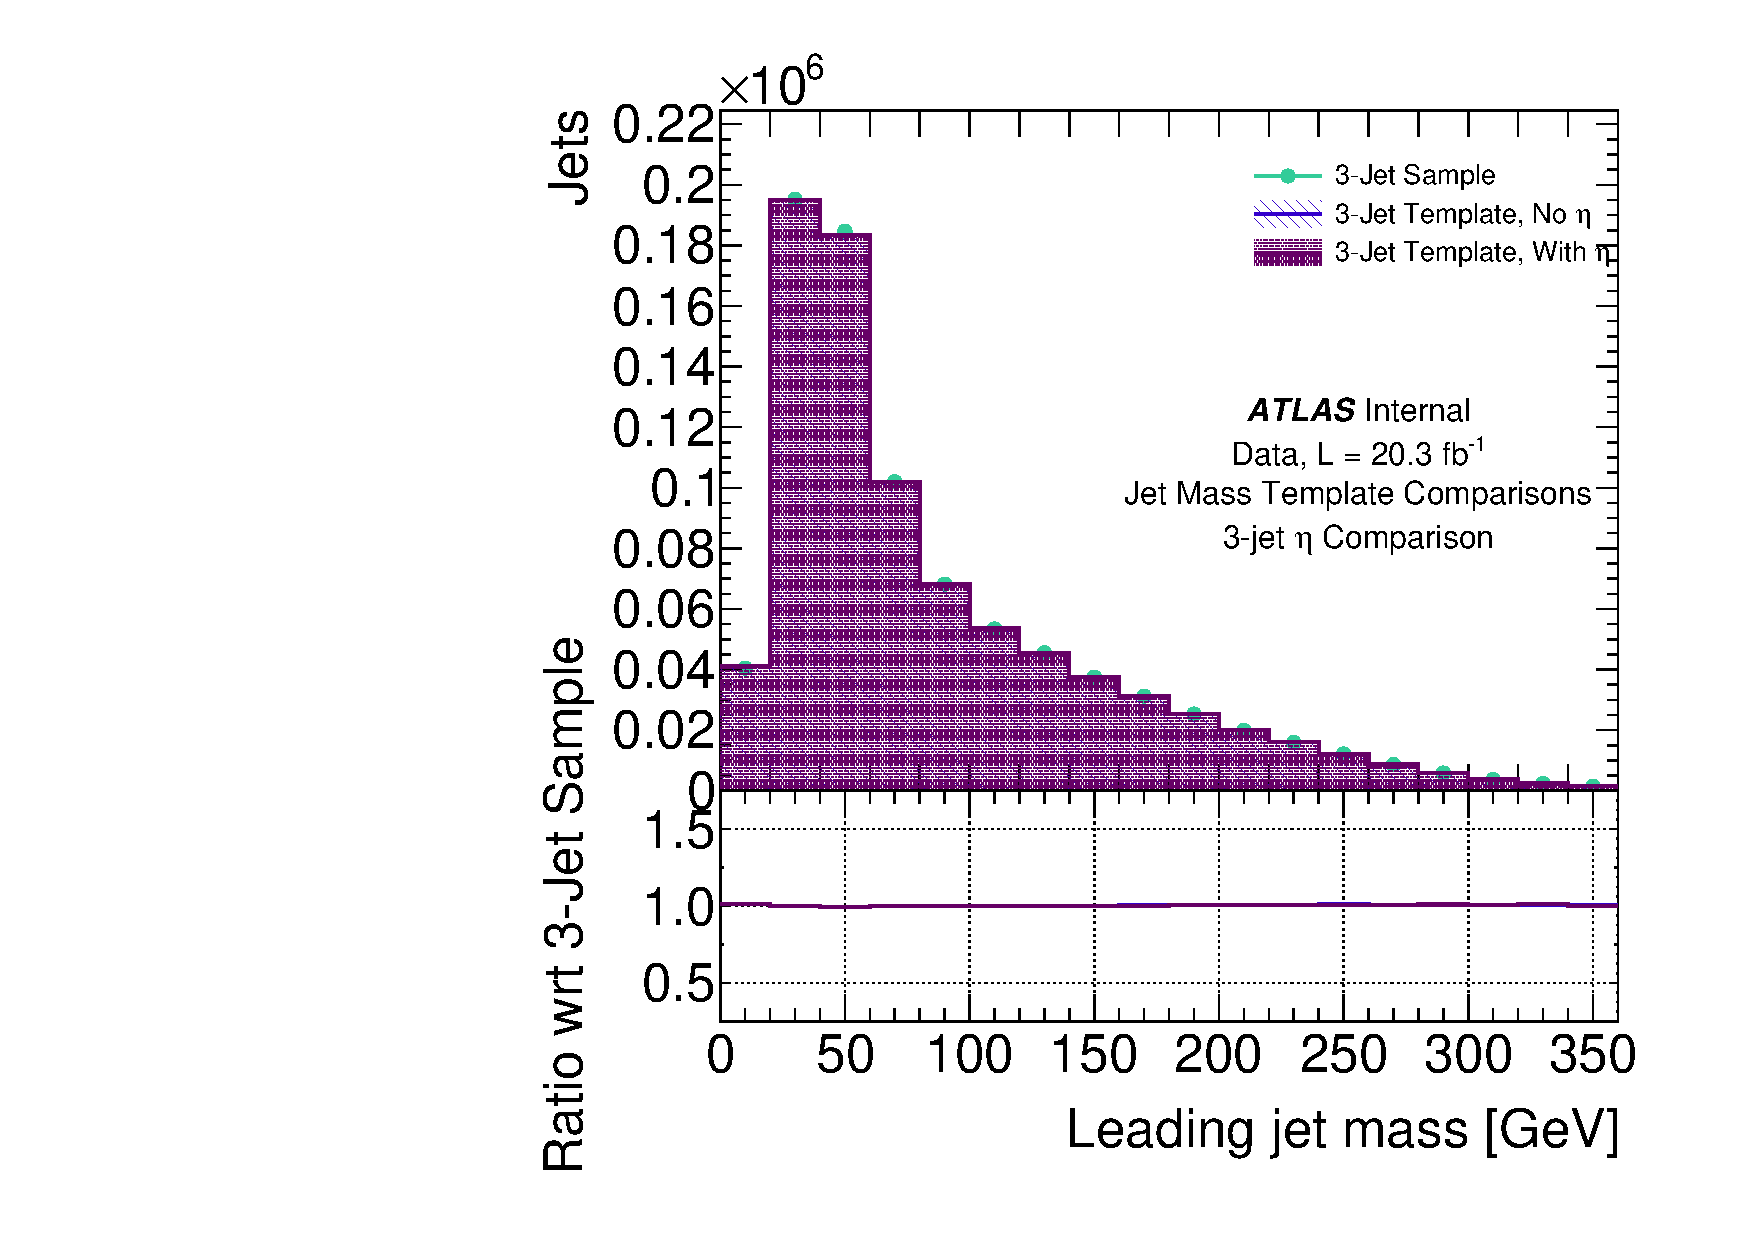
\includegraphics[width=0.3\columnwidth]{INT/Eta/jetmass1_3temp_3kin_etabinning.pdf}
    \label{fig:search:search:background:closure:inclusive}}
  \subfigure[Leading jet mass and template ($|\eta|>1.8$)]{
    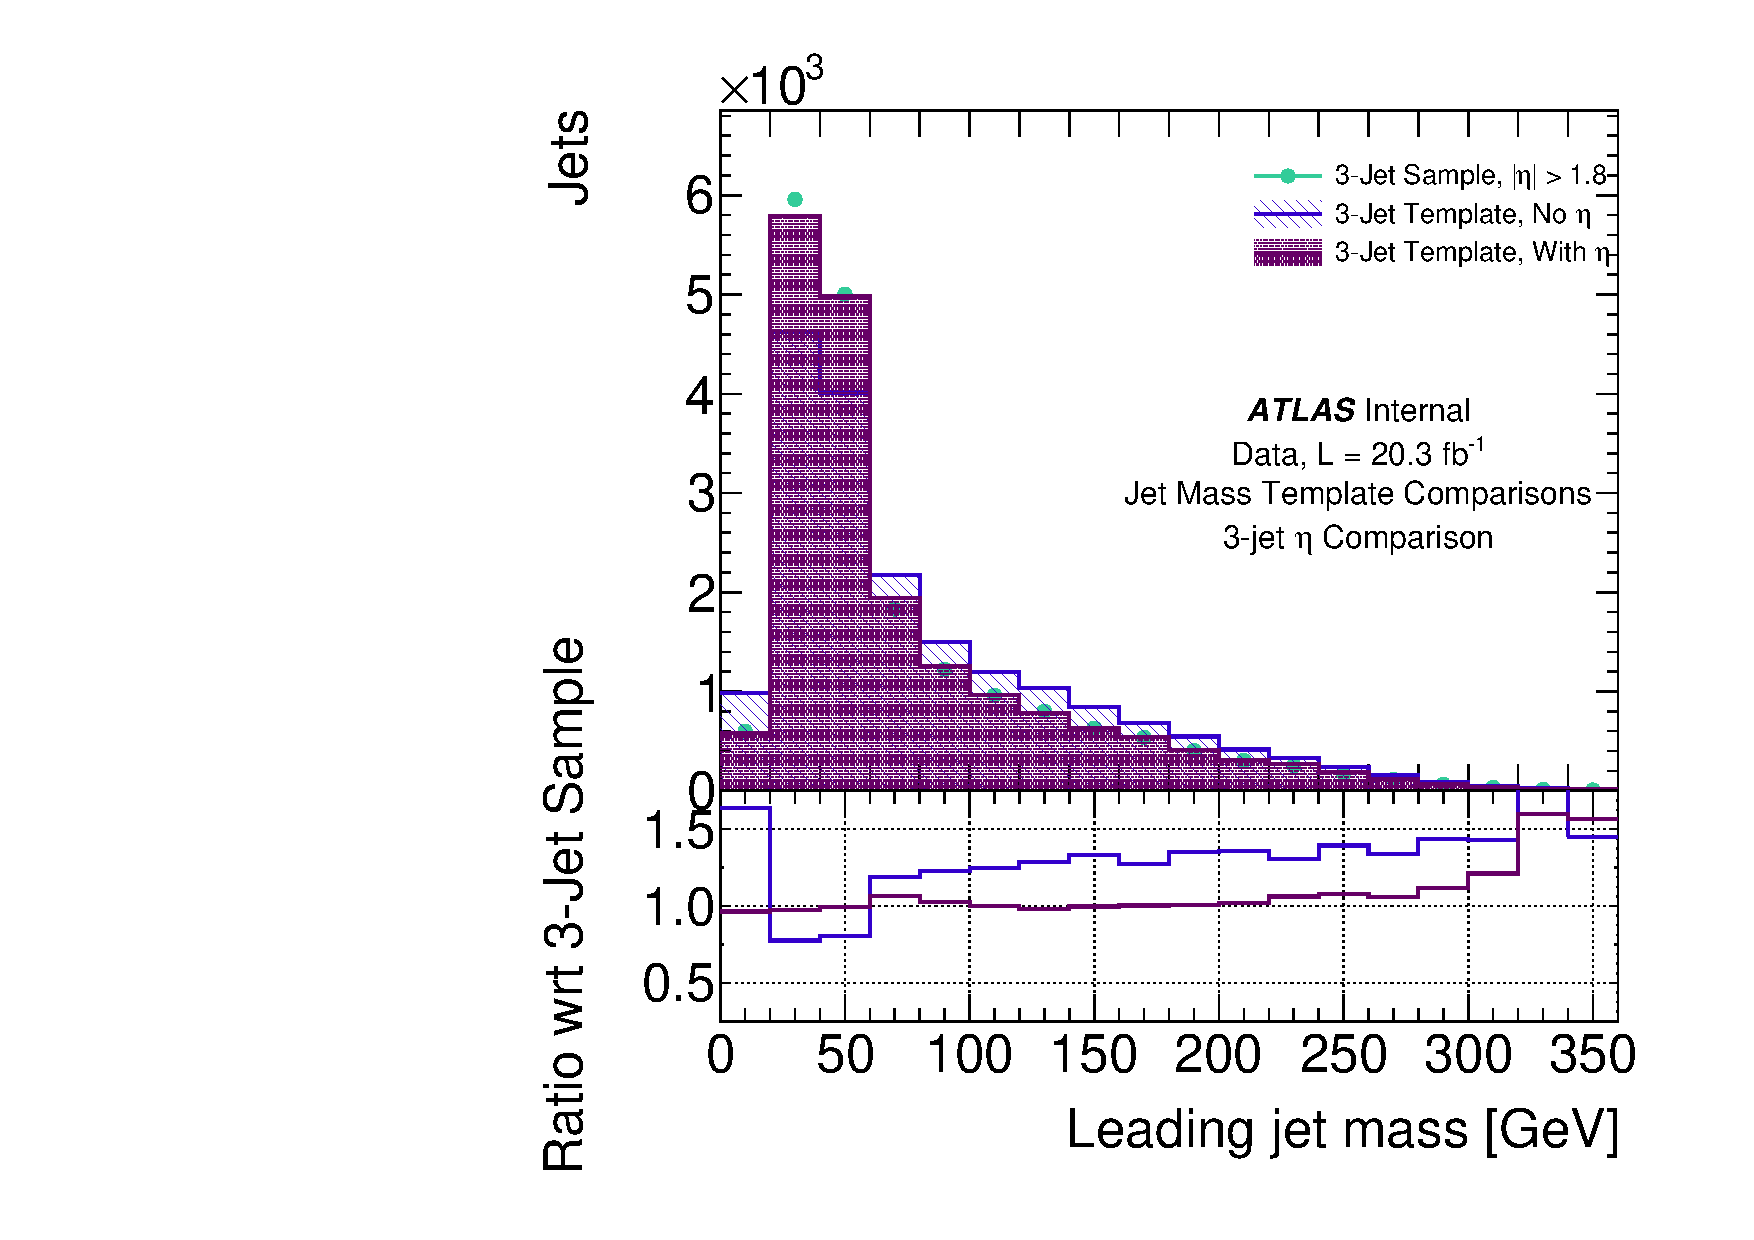
\includegraphics[width=0.3\columnwidth]{INT/Eta/jetmass1_3temp_3kin_etabinning_higheta.pdf}
    \label{fig:search:search:background:closure:higheta}} 
  \subfigure[Leading jet mass and template ($|\eta|<0.7$)]{
    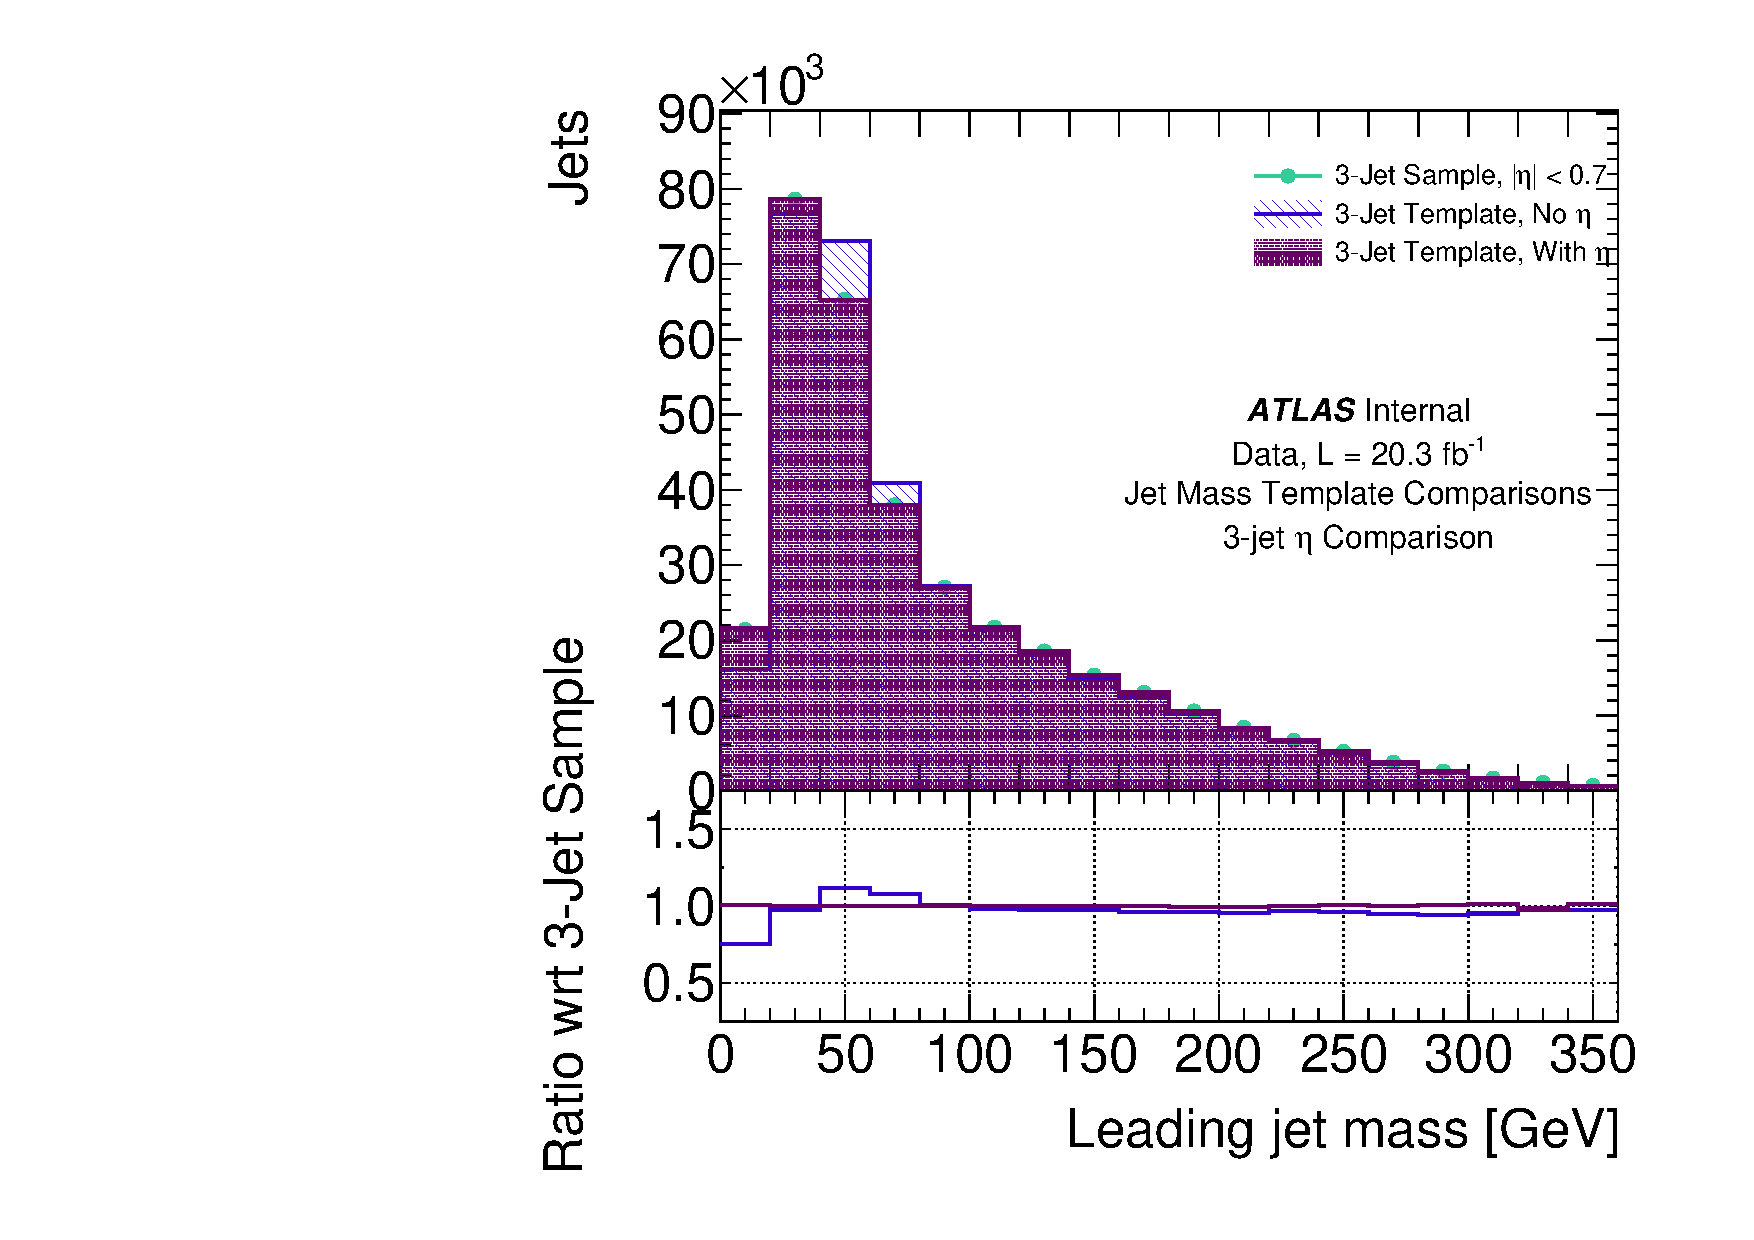
\includegraphics[width=0.3\columnwidth]{INT/Eta/jetmass1_3temp_3kin_etabinning_loweta.pdf}
    \label{fig:search:search:background:closure:loweta}} 
    
  \caption{Comparisons between templates formed with no $\eta$ dependence (dark blue) and those where the templates are formed in several jet $\eta$ bins and combined (light purple). These templates are then compared to the actual jet mass distributions for the
           \subref{fig:search:search:background:closure:inclusive} inclusive $\eta$ selection, 
           \subref{fig:search:search:background:closure:higheta} a high $\eta$ selection ($|\eta|>1.8$), and
           \subref{fig:search:search:background:closure:loweta} a low $\eta$ selection ($|\eta|<0.7$).
          }
           
  \label{fig:search:search:background:closure:eta}
\end{figure} 
%%------------------------------ 

The final closure test is to compare the \MJ template using the 3-jet kinematic sample to the actual \MJ distribution in 3-jet events. We use the approaches described above to account for $\eta$ dependence and the jet ordering. Figure~\ref{fig:search:search:background:closure:MJ} shows the closure of the method in the 3jCR using the $\ptthr>100$~GeV selection. The closure is very good, indicating that we are able to construct an event-wide variable like \MJ from the individual jet mass templates.

%%------------------------------    
\begin{figure}[!ht]
  \centering
  \includegraphics[width=0.6\columnwidth]{mj/figaux_15.pdf}
  \caption{Closure test of the \MJ template in the 3-jet control region (3jCR) using the $\ptthr>100$~GeV selection.}
  \label{fig:search:search:background:closure:MJ}
\end{figure}
%%------------------------------ 



\subsubsection{Checks on Region Compatibility}

Before extrapolating our templates to the 4j regions, it is important to first consider whether the extrapolation is sensible. If the \pt distributions are dramatically different, or the mass distributions very much different for a given \pt, then controlling for the kinematics alone will not be sufficient to build a prediction for mass. In the following plots, we show that the 3j and 4jCR have very similar 2D shapes between the input kinematics (\pt and $\eta$) and the output observable (jet mass) used in the templates. Their similar kinematic distributions means that the use of the template technique to extrapolate between them is appropriate.


Figure~\ref{fig:search:search:kincorrelations:mpt0}, for example, shows the mass-\pt correlations in the 3j and 4jCR samples in data: the distributions in fact look very similar. Likewise, Figure~\ref{fig:search:search:kincorrelations:mpt1} and Figure~\ref{fig:search:search:kincorrelations:mpt2} show these correlations for the second leading and third leading jets; again the distributions are very much compatible.

%%------------------------------    
\begin{figure}[!ht]
  \centering
  
  \subfigure[3jCR]{
    \includegraphics[width=0.48\columnwidth]{INT/kinematic_correlations/mpt_0_3.pdf}}
    % \label{fig:kincorrelations:mpt0:3}}
  \subfigure[4jCR]{
    \includegraphics[width=0.48\columnwidth]{INT/kinematic_correlations/mpt_0_4.pdf}}
    % \label{fig:kincorrelations:mpt0:4}}

    
  \caption{Leading et mass vs jet $p_T$ for the 3j and 4jCR samples.}
           
  \label{fig:search:search:kincorrelations:mpt0}
\end{figure}
%%------------------------------ 

%%------------------------------    
\begin{figure}[!ht]
  \centering
  
  \subfigure[3jCR]{
    \includegraphics[width=0.48\columnwidth]{INT/kinematic_correlations/mpt_1_3.pdf}}
    % \label{fig:kincorrelations:mpt1:3}}
  \subfigure[4jCR]{
    \includegraphics[width=0.48\columnwidth]{INT/kinematic_correlations/mpt_1_4.pdf}}
    % \label{fig:kincorrelations:mpt1:4}}

    
  \caption{Subleading jet mass vs jet $p_T$ for the 3j and 4jCR samples.}
           
  \label{fig:search:search:kincorrelations:mpt1}
\end{figure}
%%------------------------------ 


%%------------------------------    
\begin{figure}[!ht]
  \centering
  
  \subfigure[3jCR]{
    \includegraphics[width=0.48\columnwidth]{INT/kinematic_correlations/mpt_2_3.pdf}}
    % \label{fig:kincorrelations:mpt2:3}}
  \subfigure[4jCR]{
    \includegraphics[width=0.48\columnwidth]{INT/kinematic_correlations/mpt_2_4.pdf}}
    % \label{fig:kincorrelations:mpt2:4}}

    
  \caption{Third leading jet mass vs jet $p_T$ for the 3j and 4jCR samples.}
           
  \label{fig:search:search:kincorrelations:mpt2}
\end{figure}
%%------------------------------ 


Figures~\ref{fig:search:search:kincorrelations:meta0,fig:search:search:kincorrelations:meta1,fig:search:search:kincorrelations:meta2} show a similar plot displaying the correlations in mass and $\eta$. Once again, the distributions are not too different: there is no large extrapolation from a region dominated by one $\eta$ shape to a region with a different $\eta$ shape, for example.

%%------------------------------    
\begin{figure}[!ht]
  \centering
  
  \subfigure[3jCR]{
    \includegraphics[width=0.48\columnwidth]{INT/kinematic_correlations/meta_0_3.pdf}}
    % \label{fig:kincorrelations:meta0:3}}
  \subfigure[4jCR]{
    \includegraphics[width=0.48\columnwidth]{INT/kinematic_correlations/meta_0_4.pdf}}
    % \label{fig:kincorrelations:meta0:4}}

    
  \caption{Leading et mass vs jet $\eta$ for the 3j and 4jCR samples.}
           
  \label{fig:search:search:kincorrelations:meta0}
\end{figure}
%%------------------------------ 

%%------------------------------    
\begin{figure}[!ht]
  \centering
  
  \subfigure[3jCR]{
    \includegraphics[width=0.48\columnwidth]{INT/kinematic_correlations/meta_1_3.pdf}}
    % \label{fig:kincorrelations:meta1:3}}
  \subfigure[4jCR]{
    \includegraphics[width=0.48\columnwidth]{INT/kinematic_correlations/meta_1_4.pdf}}
    % \label{fig:kincorrelations:meta1:4}}

    
  \caption{Subleading jet mass vs jet $\eta$ for the 3j and 4jCR samples.}
           
  \label{fig:search:search:kincorrelations:meta1}
\end{figure}
%%------------------------------ 


%%------------------------------    
\begin{figure}[!ht]
  \centering
  
  \subfigure[3jCR]{
    \includegraphics[width=0.48\columnwidth]{INT/kinematic_correlations/meta_2_3.pdf}}
    % \label{fig:kincorrelations:meta2:3}}
  \subfigure[4jCR]{
    \includegraphics[width=0.48\columnwidth]{INT/kinematic_correlations/meta_2_4.pdf}}
    % \label{fig:kincorrelations:meta2:4}}

    
  \caption{Third leading jet mass vs jet $\eta$ for the 3j and 4jCR samples.}
           
  \label{fig:search:search:kincorrelations:meta2}
\end{figure}
%%------------------------------ 

















\subsubsection{Reweighting, and Systematic Uncertainties, in the 4jCR}

Next, we test the 3jCR templates in the 4jCR: that is, we now use the 4jCR sample's kinematics to derive a prediction for the \MJ background. Note that for this section, and most subsequent sections, we will show plots for the CR's and VR's corresponding to SR100 and SR250, but not SR1: as SR1 is a subset of SR250, the agreement (and systematic treatment) is identical to that of SR250.

The bias and variance systematics are independent, as they originate from separate sources of error in the template function, and are therefore summed in quadrature. In the individual jet mass distributions in Figure~\ref{fig:search:search:4jcr:Jets} they are shown separately, but in subsequent figures they will often be shown together to save space (though the variance is always dominant).


The template systematics are derived separately in each kinematic region where they are tested. For example, say a hypothetical training sample from which a given template is derived has the typical steeply falling jet $\pT$ spectrum over a very large range in \pT, whereas the kinematic sample to which the template is applied has only jets from $100$ GeV to $200$ GeV in $\pT$ with an approximately uniform distribution. The kinematic sample is therefore highly restricted: it will be sampling a very small region of the template formed in the training sample, and in particular, the region of the template with the highest statistics. The resulting variance of the dressed sample -- the predicted mass distribution -- will be very low, as there were many jets in the training sample from which to extrapolate. Another hypothetical kinematic sample may have only jets with $\pT > 1000$~GeV -- another very restricted sample, but one for which the training sample does not have good statistics. The resulting variance of any background prediction using this kinematic sample will thus be very large. This training sample has poorer statistics in the region where it is being used. Thus, while the variance is itself a property of the training sample, it is nonetheless affected by the choice of the kinematic sample. We see exactly this feature in Figure~\ref{fig:search:search:4jcr:Reweight:fourth}, for example: the 4th jet in the 4jCR (and all the 4j regions) is very low $\pT$, and therefore always samples the highest statistics portion of the third jet template built in the 3jCR. 

%%------------------------------    
\begin{figure}[!ht]
  \centering
  
  \subfigure[Leading jet mass and template]{
    \includegraphics[width=0.48\columnwidth]{INT/reweighting_4jet/jetmass1_3temp_4kin.pdf}
    \label{fig:search:search:4jcr:Reweight:first}}
  \subfigure[Subleading jet mass and template]{
    \includegraphics[width=0.48\columnwidth]{INT/reweighting_4jet/jetmass2_3temp_4kin.pdf}
    \label{fig:search:search:4jcr:Reweight:second}}\\
  \subfigure[Third leading jet mass and template]{
    \includegraphics[width=0.48\columnwidth]{INT/reweighting_4jet/jetmass3_3temp_4kin.pdf}
    \label{fig:search:search:4jcr:Reweight:third}}
  \subfigure[Fourth leading jet mass and template]{
    \includegraphics[width=0.48\columnwidth]{INT/reweighting_4jet/jetmass4_3temp_4kin.pdf}
    \label{fig:search:search:4jcr:Reweight:fourth}}    
    
  \caption{Comparisons between the template before and after reweighting.}
           
           
  \label{fig:search:search:4jcr:Reweight}
\end{figure}
%%------------------------------ 
%


Figure~\ref{fig:search:search:4jcr:Reweight} shows the extrapolation of the template built in the 3jCR into the 4jCR. A slight non-closure is apparent in the ratio between the observed to predicted jet mass distributions (dark blue line). Although this is not a numerically large effect in the single jet mass distributions, this non-closure can affect the total jet mass templates, and we therefore develop a reweighting procedure from the 4jCR to correct for this effect using the individual jet mass distributions for each of the four leading jets. The reweighted individual jet distributions using $\ptthr>100$~GeV are shown in Figure~\ref{fig:search:search:4jcr:Jets} --  the level of closure is improved substantially, as expected. For each of the four leading jet mass templates, the variance is substantially larger than the bias, ensuring that the estimate of the uncertainty is accurate. Figure~\ref{fig:search:search:4jcr:Jets} also shows the difference between the predicted and observed mass spectra for each jet in the cyan ratio in the bottom panels, as well as the ratio that would be obtained without any reweighting of the individual jet mass templates (dark purple). Plots for the 4jCR250 are similar, but the level of non-closure is smaller, so a reweighting is not applied (though later a systematic will still be assessed from this disagreement). %Equivalent figures showing the individual jet mass templates using the $\ptthr>250$~GeV selection are provided in \appref{templatesSR250} (see \figref{template:performance:4jcrJets:SR250}).

The reweighting applied when using the $\ptthr>100$~GeV selection accounts for the differences between the 3j and 4j samples that are due to incomplete factorization of the QCD jets in a high multiplicity final state. Two causes for the differences between the 3j and 4j samples are discussed. First, the quark/gluon composition can shift between these samples: in particular, higher multiplicity events are more likely to contain gluon jets, which on average should be more massive than light quark jets. Secondly, the 4j sample requires $\geq 4$ jets, resulting in a slightly more crowded environment than the 3j sample. Overlapping jets appear more frequently in the 4j sample as a result. Such jets tend to raise the average total jet mass, which is consistent with the observed upward shift in the templates. The reweighting factor is derived bin-by-bin as the ratio of the single jet mass template to the observed distribution in the 4jCR, and is thus a function of the jet mass. This same bin-by-bin function is applied to the 4jVR and 4jSR in subsequent plots, as noted. 


%%------------------------------    
\begin{figure}[!ht]
  \centering
  
  \subfigure[Leading jet mass and template]{
    \includegraphics[width=0.48\columnwidth]{INT/systematics_4jet/jetmass1_3temp_.pdf}
    \label{fig:search:search:4jcr:Jets:first}}
  \subfigure[Subleading jet mass and template]{
    \includegraphics[width=0.48\columnwidth]{INT/systematics_4jet/jetmass2_3temp_.pdf}
    \label{fig:search:search:4jcr:Jets:second}}\\
  \subfigure[Third leading jet mass and template]{
    \includegraphics[width=0.48\columnwidth]{INT/systematics_4jet/jetmass3_3temp_.pdf}
    \label{fig:search:search:4jcr:Jetss:third}}
  \subfigure[Fourth leading jet mass and template]{
    \includegraphics[width=0.48\columnwidth]{INT/systematics_4jet/jetmass4_3temp_.pdf}
    \label{fig:search:search:4jcr:Jets:fourth}}    
    
  \caption{Comparisons between the template derived in the 3jCR (hashed blue histogram) with the 4jCR (filled cyan circles). The ratio plot also shows the systematic uncertainty band due to the bias (in red), variance (dark purple), and the total uncertainty (in orange).}
           
  \label{fig:search:search:4jcr:Jets}
\end{figure}
%%------------------------------ 
%


Figure~\ref{fig:search:search:4jcr:Total} presents the total jet mass, \MJ, in the 4jCR using $\ptthr>100$~GeV and the $\ptthr > 250$~GeV treshhold. The nominal template (hatched histogram) includes the impact of applying the reweighting procedure to each of the input jet mass templates obtained from the dressed 4jCR sample for the CR100 case; no reweighting is applied for CR250. As with the individual jet mass, the weighted template agrees very well with the observed \MJ distribution (solid black circles) in the 4jCR.
%
%%------------------------------    
\begin{figure}[!ht]
  \centering
  \subfigure[Total jet mass in the 4jCR using $\ptthr>100$~GeV]{
    \includegraphics[width=0.48\columnwidth]{INT/systematics_4jet/jetmasstotal_3temp_.pdf}
    % \label{fig:template:performance:4jcrTotal}
  }
  \subfigure[Total jet mass in the 4jCR using $\ptthr>250$~GeV]{
    \includegraphics[width=0.48\columnwidth]{INT/pt250_cr/jetmasstotal_3temp_.pdf}
    % \label{fig:template:performance:4j250crTotal}
  }
  \caption{Total jet mass in the 4jCR with $\ptthr>100$~GeV and $\ptthr > 250$~GeV. In both cases, the reweighted template (built in the 3jCR, and applied jet-by-jet in the relevant region) is shown in the hashed blue histogram. The 4jCR templates are shown in the open blue squares. The total systematic uncertainty due to bias and variance and the non-closure in the control regions is shown in green.}
  \label{fig:search:search:4jcr:Total}
\end{figure}
%%------------------------------ 
%

It is important to emphasize that because the reweighting procedure is performed differently in the CR100 and CR250 regions, the uncertainties from the non-closure in this region are also derived slightly differently. The larger disagreement from CR100 (though not visible in Figure~\ref{fig:search:search:4jcr:Total} because the reweighting has already been applied) calls for a more conservative procedure: the full size of the reweighting is taken as an uncertainty. For the CR250,  whose disagreement is smaller but non-negligible, any significant disagreement above the existing variance is taken as an extra uncertainty. These uncertainties are summarized for both regions in Tables~\ref{tab:backSR1}, \ref{tab:backSR100}, and \ref{tab:backSR250}. All relevant uncertainties are included in Figure~\ref{fig:search:search:4jcr:Total}.



\subsubsection{Cross-checks in the 4jVR}


We test the background prediction in the 4jVR to validate the combination of the templates built in the 3jCR and the re-weighting derived in the 4jCR. As a reminder, the 4jVR requires at least 4 jets and requires that the two leading jets be separated by $1.0 < \Deta < 1.4$. The individual jet templates, before and after reweighting, are compared to the mass distributions in Figure~\ref{fig:search:search:4jvr:reweight}. In all cases, the agreement is good, especially after the application of the reweighting. The equivalent set of plots for the 4jVR250 is again very similar, and the agreement is very good. %As above, equivalent figures for templates using the $\ptthr>250$~GeV selection are again provided in \appref{templatesSR250} (see \figref{template:performance:4jvrJets:SR250}).

%%------------------------------    
\begin{figure}[!ht]
  \centering
  
  \subfigure[Leading jet mass and template]{
    \includegraphics[width=0.48\columnwidth]{INT/validation_4jet/jetmass1_3temp_4kin.pdf}
    \label{fig:template:performance:4jvrReweight:first}}
  \subfigure[Subleading jet mass and template]{
    \includegraphics[width=0.48\columnwidth]{INT/validation_4jet/jetmass2_3temp_4kin.pdf}
    \label{fig:template:performance:4jvrReweight:second}}\\
  \subfigure[Third leading jet mass and template]{
    \includegraphics[width=0.48\columnwidth]{INT/validation_4jet/jetmass3_3temp_4kin.pdf}
    \label{fig:template:performance:4jvrReweight:third}}
  \subfigure[Fourth leading jet mass and template]{
    \includegraphics[width=0.48\columnwidth]{INT/validation_4jet/jetmass4_3temp_4kin.pdf}
    \label{fig:template:performance:4jvrReweight:fourth}}    
    
  \caption{Comparisons between the templates before and after reweighting, in the 4jVR. The reweighted distributions are corrected using correction factors derived in the 4jCR, and the template is built in the 3jCR.}
               
  \label{fig:search:search:4jvr:reweight}
\end{figure}
%%------------------------------ 
%

Additionally, Figure~\ref{fig:search:search:4jvr:Total} shows the \MJ distribution in each of the validation regions, with all uncertainties shown in teal. The agreement in the validation regions is again very strong, showing the power of the template technique in estimating this complex QCD background.

%%------------------------------    
\begin{figure}[!ht]
  \centering
  \subfigure[Total jet mass in the 4jVR using $\ptthr>100$~GeV]{
    \includegraphics[width=0.48\columnwidth]{INT/validation_4jet/jetmasstotal_3temp_.pdf}
    % \label{fig:template:performance:4jvrTotal}
  }
  \subfigure[Total jet mass in the 4jVR using $\ptthr>250$~GeV]{
    \includegraphics[width=0.48\columnwidth]{INT/pt250_vr/jetmasstotal_3temp_.pdf}
    % \label{fig:template:performance:4j250vrTotal}
  }
  \caption{Total jet mass in the 4jCR with $\ptthr>100$~GeV and $\ptthr > 250$~GeV. In both cases, the reweighted template (built in the 3jCR, and applied jet-by-jet in the relevant region) is shown in the hashed blue histogram. The 4jCR templates are shown in the open blue squares. The total systematic uncertainty due to bias and variance and the non-closure in the control regions is shown in green.}
  \label{fig:search:search:4jvr:Total}
\end{figure}
%%------------------------------ 
%


\subsubsection{Final Cross-checks Using MC Simulation}
\label{chapter:search:search:mc}

One possible concern for the template technique is that it assumes that the same mechanism is responsible for generating the individual jet masses in both the control and signal regions. In the previous sections we showed the closure of the template and reweighting procedure in data (in the 4jVR region). In order to test the extent to which a different composition of processes may affect the derived templates, we relax the assumption that QCD is the only background in the 3jCR and 4j regions by injecting a sample of \Sherpa $t\bar{t}$ Monte Carlo events into the full procedure. This sample is composed of the full set of branching ratios for \ttbar\ final states. Figure~\ref{fig:search:search:mccheck:4jTop} shows the comparisons of templates in \Sherpa QCD, with and without an injection of the \ttbar\ sample. The results are consistent, showing that the background estimation is insensitive to the presence of top.

%%------------------------------    
\begin{figure}[!ht]
  \centering
  
  \subfigure[Leading jet mass]{
    \includegraphics[width=0.48\columnwidth]{INT/top_injection/jetmass1_3temp_4kin.pdf}
    \label{fig:search:search:mccheck:4jTop:first}}
  \subfigure[Subleading jet mass]{
    \includegraphics[width=0.48\columnwidth]{INT/top_injection/jetmass2_3temp_4kin.pdf}
    \label{fig:search:search:mccheck:4jTop:second}}\\
  \subfigure[Third leading jet mass]{
    \includegraphics[width=0.48\columnwidth]{INT/top_injection/jetmass3_3temp_4kin.pdf}
    \label{fig:search:search:mccheck:4jTop:third}}
  \subfigure[Fourth leading jet mass]{
    \includegraphics[width=0.48\columnwidth]{INT/top_injection/jetmass4_3temp_4kin.pdf}
    \label{fig:search:search:mccheck:4jTop:fourth}}    
    
  \caption{\ttbar\ injection tests. Comparisons of the template backgrounds in the 4jSR, for QCD only and QCD + top background distributions. The templates do not generally change with the injection of the top MC.}
               
  \label{fig:search:search:mccheck:4jTop}
\end{figure}
%%------------------------------ 



Another important test is the sensitivity of the background estimate to the presence of signal. The background expectation is derived from the kinematics of the leading 4 jets in the signal region -- if the signal affects the training sample kinematics then the background expectation for the signal region will change. We perform a direct signal injection test to determine the sensitivity of the template technique to the presence of signal. Figure~\ref{fig:search:search:mccheck:4jSignalInjection} shows the \Sherpa background estimate with and without signal events added into the full background estimation procedure. We use the $\mgluino = 600$ GeV, $\mninoone = 50$ GeV point, which shows the strongest change in the event kinematics, but the background expectation does not change.

%%------------------------------ 
\begin{figure}[!ht]
  \centering
  
  \subfigure[Leading jet mass]{
    \includegraphics[width=0.48\columnwidth]{INT/signal_injection_sr/jetmass1_3temp_4kin.pdf}
    \label{fig:search:search:mccheck:4jSignalInjection:first}}
  \subfigure[Subleading jet mass]{
    \includegraphics[width=0.48\columnwidth]{INT/signal_injection_sr/jetmass2_3temp_4kin.pdf}
    \label{fig:search:search:mccheck:4jSignalInjection:second}}\\
  \subfigure[Third leading jet mass]{
    \includegraphics[width=0.48\columnwidth]{INT/signal_injection_sr/jetmass3_3temp_4kin.pdf}
    \label{fig:search:search:mccheck:4jSignalInjection:third}}
  \subfigure[Fourth leading jet mass]{
    \includegraphics[width=0.48\columnwidth]{INT/signal_injection_sr/jetmass4_3temp_4kin.pdf}
    \label{fig:search:search:mccheck:4jSignalInjection:fourth}}    
    
  \caption{Signal injection tests. Comparisons of the template backgrounds in the 4jSR, with and without signal injection. We use the $\mgluino = 600$ GeV, $\mninoone = 50$ GeV point, which shows the strongest kinematic differences with the background sample. The resulting background expectation does not change.}
               
  \label{fig:search:search:mccheck:4jSignalInjection}
\end{figure}
%%------------------------------ 

Finally, Figure~\ref{fig:search:search:mccheck:4jSherpa} shows the closure test of the technique in Sherpa QCD alone (with no other injection). This plot shows that the agreement, after the full procedure of template derivation and reweighting, succeeds in the MC signal region. 

%%------------------------------ 
\begin{figure}[!ht]
  \centering
  
  \subfigure[Leading jet mass]{
    \includegraphics[width=0.48\columnwidth]{INT/sherpa_test/jetmass1_3temp_4kin_closure.pdf}
    \label{fig:search:search:mccheck:4jSherpa:first}}%
  \subfigure[Subleading jet mass]{
    \includegraphics[width=0.48\columnwidth]{INT/sherpa_test/jetmass2_3temp_4kin_closure.pdf}
    \label{fig:search:search:mccheck:4jSherpa:second}}
  \subfigure[Third leading jet mass]{
    \includegraphics[width=0.48\columnwidth]{INT/sherpa_test/jetmass3_3temp_4kin_closure.pdf}
    \label{fig:search:search:mccheck:4jSherpa:third}}%
  \subfigure[Fourth leading jet mass]{
    \includegraphics[width=0.48\columnwidth]{INT/sherpa_test/jetmass4_3temp_4kin_closure.pdf}
    \label{fig:search:search:mccheck:4jSherpa:fourth}}
    
  \caption{Sherpa closure test of the template + reweighting technique. The individual jet masses are shown in the SR, compared to the prediction before and after reweighting. The reweighted sample shows good agreement with the observed distribution.}
               
  \label{fig:search:search:mccheck:4jSherpa}
\end{figure}
%%------------------------------ 



\subsubsection{Uncertainties}


The systematic uncertainties affecting the analysis fall into two broad categories: those that derive from the selections and background estimations of the analysis itself, and those that affect the predicted signal properties and selection efficiencies. Each of these two categories are discussed in the following sections.

%%------------------------------ 
\subsubsection{Template-based background estimation uncertainties}
%%------------------------------ 


As described in Section~\ref{chapter:search:substructure:templates} above, there are two systematic sources of error associated with the template procedure: the uncertainty due to finite statistics in the training sample (called the variance), and the uncertainty due to the smoothing procedure in the template derivation (called the bias). All plots of the total jet mass distributions shown include both the variance and bias in the systematics. The bias is nominally treated as a fully correlated bin-by-bin uncertainty in the multi-bin fit: the degree of over-smoothing affects all bins simultaneously, if it affects any.

To assess the degree of correlation between bins, we explicitly construct the \textit{covariance matrix}, where $v_i$ is the vector corresponding to the background estimate bins, and $i$ iterates over bins, as
%
%----------------
\begin{equation}
C_{ij} = \overline{v_i v_j} - (\overline{v_i}\,\, \overline{v_j}),
\end{equation}
%----------------
%
\noindent and the correlation matrix as
%
%----------------
\begin{equation}
C'_{ij} = \frac{\overline{v_i v_j }}{\sigma_i \sigma_j} - \frac{\overline{v_i}\,\,\overline{v_j}}{\sigma_i \sigma_j}.
\end{equation}
%----------------
%
\noindent The correlation matrix for SR250 is shown in Figure~\ref{fig:search:search:systematics:SR250}. Only a mild correlation exists between neighboring bins, and only one out of ten independent off-diagonal elements has a correlation greater than 20\%, only two have greater than 10\%, and the remaining are a the percent or sub-percent level. One option to reduce the number of Nuisance Parameters is to diagonalize the covariance matrix, and drop the subdominant (normalized) eigenvalues/vectors. The diagonalization procedure, however, reveals that the preferred eigenbasis is very close to that of the diagonal, which is sensible given the very small degree of correlation. For this reason, we apply the variation of each bin independently, assigning a nuisance parameter to each bin separately. This has the added benefit of reducing the profiling during the fit (as there are now more Nuisance Parameters than fit points). The effect on the limit is modest, and the exclusion reach and sensitivity of the analysis does not change appreciably.


% Both systematics are (separately) treated as correlated bin-by-bin in the multi-bin fits. Assessments of the individual toys used to estimate the variance show that fluctuations in the 3jCR (the source of the variance systematic) create systematic shifts in the \MJ distribution-- not solitary spikes which would require an uncorrelated bin-by-bin approach. The kernel smoothing procedure spreads flucutations in the templates across many bins, and so it is reasonable to expect a fully correlated systematic bin-by-bin.

% \Figref{systematics:toys} shows an example of why this is the case. The figure shows the \MJ distribution from two (out of 100) toys used to calculate the variance. Both are the result of a Poisson-fluctuated dataset in the 3jCR. The fluctations of the black toy did not spikes in comparison to the red toy, but instead a systematic shift in a single direction, caused by the inherent smoothing procedure in the template method. This shows the need to use correlated bins to assess the variance systematic.

% %%------------------------------    
% \begin{figure}[!ht]
%   \centering  
%   \includegraphics[width=0.65\columnwidth]{figures/Systematics/c1.eps}
%   \caption{Example of two statistical toys used to calculate the variance of the template method. The toy in black is consistently shifted to the right-- the fluctuations in the 3jCR where the template was constructed results in a systematic shift of the \MJ distribution, and show the need to use correlated bins to describe the variance systematic.}
%   \label{fig:systematics:toys}
% \end{figure}
% %%------------------------------

%%------------------------------    
\begin{figure}[!ht]
  \centering
  
  \subfigure[Covariance Matrix]{
    \includegraphics[width=0.48\columnwidth]{INT/Systematics/Cov/CovarianceSR250.pdf}
    \label{fig:search:search:systematics:SR250:covariance}}
  %  
  \subfigure[Correlation Matrix]{
    \includegraphics[width=0.48\columnwidth]{INT/Systematics/Cov/CorrelationSR250.pdf}
    \label{fig:search:search:systematics:SR250:correlation}}
    
  \caption{Correlation and covariance matrix for SR250. The correlation matrix reveals that the correlation amongst bins is rather small, and suggest the usage of 5 separate nuisance parameters for SR250. The 5 bins here indicate the last 5 bins of the SR250 distributions.}
           
  \label{fig:search:search:systematics:SR250}
\end{figure}
%%------------------------------ 

A third systematic, applicable to all signal regions, is the size of the reweighting applied (or the observed non-closure compared to data) to the total jet mass prediction, as derived in the 4jCR. This is also treated as fully correlated between the bins used in the multi-bin fit.  For all but the lowest \MJ bin in SR100, the reweighting systematic dominates. The SR250 and single-bin signal regions, when tested in the 4jCR and 4jVR, revealed a significantly smaller non-closure, and thus no reweighting is applied. The small levels of significant residual non-closure observed in the 4jCR is applied as a systematic to cover any remaining disagreement between data and prediction. At low values of \MJ this can dominate, but becomes subdominant at higher values of \MJ.

The set of tables provided in Table~\ref{tab:backSR1}, Table~\ref{tab:backSR100}, and Table~\ref{tab:backSR250} provide a full breakdown of the systematics in the background estimates for all signal regions.

%%------------------------------    
\begin{table}[!ht]
\begin{center}\renewcommand\arraystretch{1.6}
\begin{tabular}{r|l}

  
\multicolumn{2}{c}{Uncertainties in single bin region} \\
\hline \hline

$\mathbf{\MJ}$ \textbf{Bin [GeV]}  & $\mathbf{\geq 625}$ \\
\hline
 Expected Number of Events & 164 $\pm 13$  \\
 Variance & +26\% / -20\% \\
 Bias & $\pm 8$\% \\
 4jCR Difference  & $\pm 7$\% \\
 \hline \hline
  \end{tabular}
  
  \caption{Expected number of observed events, and the systematic uncertainty from the template method, for the single bin signal region characterized by $\MJ \geq 625$~GeV and $\pt^{3}>250$~GeV. \label{tab:backSR1}}
\end{center}
\end{table}
%%------------------------------ 


%%------------------------------    
\begin{table}[!ht]
\begin{center}\renewcommand\arraystretch{1.6}
\begin{tabular}{r|l |l |l |l |l }

  
\multicolumn{6}{c}{Uncertainties in SR100} \\
\hline \hline

$\mathbf{\MJ}$ \textbf{Bin [GeV]}  & \textbf{350 - 400} & \textbf{400 - 450} & \textbf{450 - 525} & \textbf{525 - 725} & $\mathbf{>725}$ \\ \cline{2-6}
\hline
 Expected Number of Events & $4250\pm78$ & $2640\pm49$ & $2070\pm42$ & $965\pm24$ & $71\pm7$ \\
 Variance & +3\% / -2\% & +2\% / -3\% & +4\% / -4\% & +7\% / -7\% & +37\% / - 38\% \\
 Bias & $\pm$1\% & $\pm$1\% & $\pm$1\% & $\pm$2\% & $\pm$15\% \\
 Reweighting& $\pm$12\% & $\pm$14\% & $\pm$17\% & $\pm$20\% & $\pm$22\% \\
 \hline \hline
  \end{tabular}
  
  \caption{Expected number of observed events, and the systematic uncertainty from the template method, for the SR100 signal region. \label{tab:backSR100}}
\end{center}
\end{table}
%%------------------------------ 

%%------------------------------    
\begin{table}[!ht]
\begin{center}\renewcommand\arraystretch{1.6}
\begin{tabular}{r|l |l |l |l |l }

  
\multicolumn{6}{c}{Uncertainties in SR250} \\
\hline \hline

$\mathbf{\MJ}$ \textbf{Bin [GeV]}  & \textbf{350 - 400} & \textbf{400 - 450} & \textbf{450 - 525} & \textbf{525 - 725} & $\mathbf{>725}$ \\ \cline{2-6}
\hline
 Expected Number of Events & $1430\pm35$ & $920\pm33$ & $780\pm32$ & $490\pm23$ & $37\pm6$ \\
 Variance & +3\% / -4\% & +5\% / -5\% & +5\% / -5\% & +10\% / -9\% & +45\% / - 31\% \\
 Bias & $\pm$2\% & $\pm$1\% & $\pm$1\% & $\pm$3\% & $\pm$15\% \\
 4jCR Difference & $\pm$8\% & $\pm$14\% & $\pm$11\% & $\pm$10\% & $\pm$7\% \\
 \hline \hline
  \end{tabular}
  
  \caption{Expected number of observed events, and the systematic uncertainty from the template method, for the SR250 signal region. \label{tab:backSR250}}
\end{center}
\end{table}
%%------------------------------ 





%%------------------------------ 
\subsubsection{Signal systematic uncertainties and measurement uncertainties}
%%------------------------------ 

Uncertainties must also be assessed on the selection efficiency for each signal model considered in the analysis. The uncertainty is dominated by the jet energy scale (JES) and jet mass scale (JMS) uncertainties. In particular, the JMS uncertainty affects the selection efficiency significantly and results in the largest single source of measurement uncertainties associated with the signal. A breakdown of the JES and JMS uncertainties in the different signal regions is shown in Tables~\ref{tab:jesjms:SR1},~\ref{tab:jesjms:SR100},~and~\ref{tab:jesjms:SR250}. 
%
Note that the JES and JMS are assessed independently, and assumed therefore to be uncorrelated. Studies were done to correlate/anti-correlate the uncertainties and assess the change: as the differences were not large, we maintain the nominal uncorrelated assumption here.
%
The JMS is by far the largest systematic for all signal points. The JES is negligible for the single bin and SR100 signal regions, but becomes a little larger for the SR250 signal region (which cuts more strongly on the 3rd jet \pT, and is therefore expected to be more significantly affected by the JES).

%%------------------------------    
\begin{figure}[!ht]
  \centering
  
  \subfigure[Impact of JES on \MJ]{
    \includegraphics[width=0.48\columnwidth]{INT/Systematics/overlay_MJ4_Syst_HiFat_JES_hpp_RPVGluinoToChi_10q_M800_300_j470_AntiKt10LCTopoTrimmedPtFrac5SmallR30_data12_v\PlotVersion.pdf}
    \label{fig:jesjms:jes:MJ}}
  %  
  \subfigure[Impact of JES on \Deta]{
    \includegraphics[width=0.48\columnwidth]{INT/Systematics/overlay_DEta_Syst_HiFat_JES_hpp_RPVGluinoToChi_10q_M800_300_j470_AntiKt10LCTopoTrimmedPtFrac5SmallR30_data12_v\PlotVersion.pdf}
    \label{fig:jesjms:jes:DEta}}
    
  \caption{Impact of the jet energy scale systematic uncertainty on the \MJ and \Deta distributions for an inclusive event selection, on the \mgluino = 800 GeV, \mninoone = 300 GeV mass point.
           }
           
  \label{fig:jesjms:jes}
\end{figure}
%%------------------------------ 


%%------------------------------    
\begin{figure}[!ht]
  \centering
  
  \subfigure[Impact of JMS on \MJ]{
    \includegraphics[width=0.48\columnwidth]{INT/Systematics/overlay_MJ4_Syst_HiFat_JMS_hpp_RPVGluinoToChi_10q_M800_300_j470_AntiKt10LCTopoTrimmedPtFrac5SmallR30_data12_v\PlotVersion.pdf}
    \label{fig:jesjms:jms:MJ}}
  %  
  \subfigure[Impact of JMS on \Deta]{
    \includegraphics[width=0.48\columnwidth]{INT/Systematics/overlay_DEta_Syst_HiFat_JMS_hpp_RPVGluinoToChi_10q_M800_300_j470_AntiKt10LCTopoTrimmedPtFrac5SmallR30_data12_v\PlotVersion.pdf}
    \label{fig:jesjms:jms:DEta}}
    
  \caption{Impact of the jet mass scale systematic uncertainty on the \MJ and \Deta distributions for an inclusive event selection, on the \mgluino = 800 GeV, \mninoone = 300 GeV mass point.
           }
           
  \label{fig:jesjms:jms}
\end{figure}
%%------------------------------ 


% %%------------------------------    
% \begin{figure}[!ht]
%   \centering
  
%   \subfigure[Impact of JMS on \MJ]{
%     \includegraphics[width=0.48\columnwidth]{figures/Systematics/overlay_MJ4_Syst_HiFat_JMS_hpp_RPVGluinoToChi_10q_M800_300_j470_AntiKt10LCTopoTrimmedPtFrac5SmallR30_data12_v\PlotVersion.pdf}
%     \label{fig:jesjms:jms:MJ}
%     }
%   %  
%   \subfigure[Impact of JMS on \DEta]{
%     \includegraphics[width=0.48\columnwidth]{figures/Systematics/overlay_DEta_Syst_HiFat_JMS_hpp_RPVGluinoToChi_10q_M800_300_j470_AntiKt10LCTopoTrimmedPtFrac5SmallR30_data12_v\PlotVersion.pdf}
%     \label{fig:jesjms:jms:DEta}
%     }
    
%   \caption{Impact of the jet mass scale systematic uncertainty on the \MJ and \Deta distributions for an inclusive event selection, on the \mgluino = 800 GeV, \mninoone = 300 GeV mass point.
%            }
           
%   \label{fig:jesjms:jms}
% \end{figure}
% %%------------------------------ 

\begin{table}[!ht]
%\footnotesize
\begin{center}\renewcommand\arraystretch{1.6}
\begin{tabular}{r|l |l |l |l |l }

\hline \hline
\multicolumn{6}{c}{\textbf{Single Bin, \MJ $>$ 625 GeV}} \\
\hline \hline

{\mgluino, \mninoone [GeV]}  & 600, 50 & 800, 175 & 1000, 300 & 1200, 600 & 1400, 50 \\ \cline{2-6}
\hline
JES & $\pm$ 4\% & $\pm$ 4\% & $\pm$ 2\% & $\pm$ 1\% & $\pm$ 1\%  \\
JMS & $\pm$ 34\% & $\pm$ 28\% & $\pm$ 19\% & $\pm$ 13\% & $\pm$ 14\% \\
\hline \hline

\end{tabular}
\caption{Breakdown of JES and JMS for the single-bin signal region characterized by $\MJ \geq 625$~GeV and $\pt^{3}>250$~GeV.}\label{tab:jesjms:SR1}
\end{center}
\end{table}

\begin{table}[!ht]
%\footnotesize
\begin{center}\renewcommand\arraystretch{1.6}
\begin{tabular}{r|l |l |l |l |l }

\hline \hline
\multicolumn{6}{c}{\textbf{Multi-Bin, JMS, SR100}} \\
\hline \hline

{\bfseries \MJ Bin [GeV]}  & 350 - 400 & 400 - 450 & 450 - 525 & 525 - 725 & $>$725 \\ \cline{2-6}
\hline
 \mgluino = 600,  \mninoone = 50 GeV &  $\pm 11$\% & $\pm 9$\% & $\pm 7$\% & $\pm 20$\% & $\pm 50$\%  \\
 \mgluino = 800,  \mninoone = 175 GeV & $\pm 20$\% & $\pm 11$\% & $\pm 11$\% & $\pm 12$\% & $\pm 37$\%  \\
 \mgluino = 1000,  \mninoone = 300 GeV & $\pm 25$\% & $\pm 17$\% & $\pm 13$\% & $\pm 21$\% & $\pm 29$\%  \\
 \mgluino = 1200,  \mninoone = 600 GeV & $\pm 26$\% & $\pm 27$\% & $\pm 18$\% & $\pm 19$\% & $\pm 20$\%  \\
 \mgluino = 1400,  \mninoone = 50 GeV & $\pm 12$\% & $\pm 2$\% & $\pm 2$\% & $\pm 1$\% & $\pm 19$\%  \\
\hline \hline

\multicolumn{6}{c}{\textbf{Multi-Bin, JES, SR100}} \\
\hline \hline

{\bfseries \MJ Bin [GeV]}  & 350 - 400 & 400 - 450 & 450 - 525 & 525 - 725 & $>$725 \\ \cline{2-6}
\hline
 \mgluino = 600,  \mninoone = 50 GeV &  $\pm 4$\% & $\pm 4$\% & $\pm 4$\% & $\pm 4$\% & $\pm 3$\%  \\
 \mgluino = 800,  \mninoone = 175 GeV & $\pm 3$\% & $\pm 4$\% & $\pm 3$\% & $\pm 5$\% & $\pm 3$\%  \\
 \mgluino = 1000,  \mninoone = 300 GeV & $\pm 1$\% & $\pm 1$\% & $\pm 2$\% & $\pm 2$\% & $\pm 2$\%  \\
 \mgluino = 1200,  \mninoone = 600 GeV & $\pm 0$\% & $\pm 1$\% & $\pm 1$\% & $\pm 1$\% & $\pm 2$\%  \\
 \mgluino = 1400,  \mninoone = 50 GeV & $\pm 1$\% & $\pm 0$\% & $\pm 1$\% & $\pm 1$\% & $\pm 1$\%  \\
\hline \hline

\end{tabular}
\caption{Breakdown of JES and JMS for the multi-bin SR100 signal region.}\label{tab:jesjms:SR100}
\end{center}
\end{table}


\begin{table}[!ht]
%\footnotesize
\begin{center}\renewcommand\arraystretch{1.6}
\begin{tabular}{r|l |l |l |l |l }

\hline \hline
\multicolumn{6}{c}{\textbf{Multi-Bin, JMS, SR250}} \\
\hline \hline

{\bfseries \MJ Bin [GeV]}  & 350 - 400 & 400 - 450 & 450 - 525 & 525 - 725 & $>$725 \\ \cline{2-6}
\hline
 \mgluino = 600,  \mninoone = 50 GeV &  $\pm 9$\% & $\pm 5$\% & $\pm 12$\% & $\pm 18$\% & $\pm 41$\%  \\
 \mgluino = 800,  \mninoone = 175 GeV & $\pm 23$\% & $\pm 18$\% & $\pm 14$\% & $\pm 10$\% & $\pm 37$\%  \\
 \mgluino = 1000,  \mninoone = 300 GeV & $\pm 25$\% & $\pm 19$\% & $\pm 14$\% & $\pm 22$\% & $\pm 29$\%  \\
 \mgluino = 1200,  \mninoone = 600 GeV & $\pm 26$\% & $\pm 28$\% & $\pm 19$\% & $\pm 19$\% & $\pm 20$\%  \\
 \mgluino = 1400,  \mninoone = 50 GeV & $\pm 13$\% & $\pm 1$\% & $\pm 2$\% & $\pm 2$\% & $\pm 20$\%  \\
\hline \hline

\multicolumn{6}{c}{\textbf{Multi-Bin, JES, SR250}} \\
\hline \hline

{\bfseries \MJ Bin [GeV]}  & 350 - 400 & 400 - 450 & 450 - 525 & 525 - 725 & $>$725 \\ \cline{2-6}
\hline
 \mgluino = 600,  \mninoone = 50 GeV &  $\pm 15$\% & $\pm 12$\% & $\pm 12$\% & $\pm 11$\% & $\pm 10$\%  \\
 \mgluino = 800,  \mninoone = 175 GeV & $\pm 10$\% & $\pm 10$\% & $\pm 10$\% & $\pm 8$\% & $\pm 7$\%  \\
 \mgluino = 1000,  \mninoone = 300 GeV & $\pm 8$\% & $\pm 8$\% & $\pm 7$\% & $\pm 6$\% & $\pm 5$\%  \\
 \mgluino = 1200,  \mninoone = 600 GeV & $\pm 5$\% & $\pm 5$\% & $\pm 5$\% & $\pm 4$\% & $\pm 3$\%  \\
 \mgluino = 1400,  \mninoone = 50 GeV & $\pm 1$\% & $\pm 2$\% & $\pm 1$\% & $\pm 2$\% & $\pm 2$\%  \\
\hline \hline

\end{tabular}
\caption{Breakdown of JES and JMS for the multi-bin SR250 signal region.}\label{tab:jesjms:SR250}
\end{center}
\end{table}









An additional pair of systematics comes from the effects of the Jet Energy Resolution (JER) and Jet Mass Resolution (JMR). The jet substructure group does not release an official set of resolutions, but instead prescribes a set of studies for measuring the resolution in MC samples. They yield the fitted resolution functions seen in Figure~\ref{fig:res}.
%
%%------------------------------    
\begin{figure}[!ht]
  \centering
  
  \subfigure[Energy Resolution]{
    \includegraphics[width=0.48\columnwidth]{INT/Resolution/Response_vs_ptEnergy_0_0.pdf}
    \label{fig:res:jer}}
  %  
  \subfigure[Mass Resolution]{
    \includegraphics[width=0.48\columnwidth]{INT/Resolution/Response_vs_ptMass_0_0.pdf}
    \label{fig:res:jmr}}
    
  \caption{Fitted resolution functions, as a function of $p_{T}$, for all signal MC.
           }
           
  \label{fig:res}
\end{figure}
%%------------------------------ 
%
To estimate the uncertainty due to possible disagreement between data and MC simulation, this measured resolution and smear the \pT\ and mass of the jet such that it increases by $20\%$. This factor of $20\%$ is very roughly derived from the disagreement between data and MC in describing the $W$ mass peak from \ttbar events; as this is only valid in a very limited \pt range, the value is inflated significantly and extrapolated to the full phase space. In practice, this means applying a Gaussian smearing with mean $m$ and $\sigma = 0.66\sigma^{measured}$. We apply this smearing to all of our signal grid points.\footnote{Due to a large sensitivity to statistical uncertainty in this procedure, and the fact that mass distributions vary little for different values of \mninoone for constant \mgluino, we merge some signal distributions across \mninoone bins in order to increase statistics.} %The results of the JMR smearing are displayed in \figref{res:jmrresult}.
%


Table~\ref{tab:jerjmr:SR1}, \ref{tab:jerjmr:SR100}, and \ref{tab:jerjmr:SR250} show a summary of the JER and JMR for several mass points. Generally the systematic is very low -- the effect of the JER is not observable, and the JMR is always subdominant to the JES and less than $10\%$.

% %%------------------------------    
% \begin{figure}[!ht]
%   \centering
  
%   \subfigure[SR1]{
%     \includegraphics[width=0.45\columnwidth]{figures/Resolution/jmrSR0.pdf}
%     \label{fig:res:jmr1}}
%   %  
%   \subfigure[SR2]{
%     \includegraphics[width=0.45\columnwidth]{figures/Resolution/jmrSR1.pdf}
%     \label{fig:res:jmr2}}
%   % 
%   \subfigure[SR3]{
%     \includegraphics[width=0.45\columnwidth]{figures/Resolution/jmrSR2.pdf}
%     \label{fig:res:jmr3}}
    
%   \caption{Size of the jet resolution systematic on the signal acceptance in each SR.
%            }
           
%   \label{fig:res:jmrresult}
% \end{figure}
% %%------------------------------ 

\begin{table}[!ht]
%\footnotesize
\begin{center}\renewcommand\arraystretch{1.6}
\begin{tabular}{r|l |l |l |l |l }

\hline \hline
\multicolumn{6}{c}{\textbf{Single Bin, \MJ $>$ 625 GeV}} \\
\hline \hline

{\mgluino, \mninoone [GeV]}  & 600, 50 & 800, 175 & 1000, 300 & 1200, 600 & 1400, 50 \\ \cline{2-6}
\hline
JER & $\pm$0\% & $\pm$0\% & $\pm$0\% & $\pm$0\% & $\pm$0\%\ \\
JMR & $\pm$4\% & $\pm$5\% & $\pm$0\% & $\pm$1\% & $\pm$1\% \\

% \hline \hline
% \multicolumn{6}{c}{\textbf{Signal Region 2 (SR2)}} \\
% \hline \hline

% {\bfseries \mgluino, \mninoone}  & 600, 50 & 800, 175 & 1000, 300 & 1200, 600 & 1400, 50 \\ \cline{2-6}
% \hline
% %JER & +1.9\%\, -5.2\% & +3.0\%\, -3.4\% & \textbf{+2.0\%\, -2.2\%} & \textbf{+0.9\%\, -1.2\%} & +1.5\%\, -1.5\%  \\
% JER & +0\% & 0\% & \textbf{-0\%} & \textbf{+0\%} & 0\%\ \\
% JMR & 27\% & +18\% & \textbf{+9\%} & \textbf{-1\%} & +0\% \\

% \hline \hline
% \multicolumn{6}{c}{\textbf{Signal Region 3 (SR3)}} \\
% \hline \hline

% {\bfseries \mgluino, \mninoone}  & 600, 50 & 800, 175 & 1000, 300 & 1200, 600 & 1400, 50 \\ \cline{2-6}
% \hline
% JER & +2\% & 0\% & 0\% & +0\% & \textbf{-0\%}\ \\
% JMR & +39\% & +40\% & +23\% & +14\% & \textbf{+12\%} \\

\hline \hline

\end{tabular}
\caption{Breakdown of JER and JMR for a few mass points in the SR250 Signal Region, with a single bin cut of $\MJ > 650$ GeV.}\label{tab:jerjmr:SR1}
\end{center}
\end{table}



\begin{table}[!ht]
%\footnotesize
\begin{center}\renewcommand\arraystretch{1.6}
\begin{tabular}{r|l |l |l |l |l }

\hline \hline
\multicolumn{6}{c}{\textbf{Multi-Bin, JMR, SR100}} \\
\hline \hline

{\bfseries \MJ Bin [GeV]}  & 350 - 400 & 400 - 450 & 450 - 525 & 525 - 725 & $>$725 \\ \cline{2-6}
\hline
 \mgluino = 600,  \mninoone = 50 GeV &  $\pm 4$\% & $\pm 1$\% & $\pm 0$\% & $\pm 0$\% & $\pm 1$\%  \\
 \mgluino = 800,  \mninoone = 175 GeV & $\pm 4$\% & $\pm 1$\% & $\pm 2$\% & $\pm 3$\% & $\pm 9$\%  \\
 \mgluino = 1000,  \mninoone = 300 GeV & $\pm 4$\% & $\pm 1$\% & $\pm 0$\% & $\pm 3$\% & $\pm 3$\%  \\
 \mgluino = 1200,  \mninoone = 600 GeV & $\pm 6$\% & $\pm 5$\% & $\pm 1$\% & $\pm 2$\% & $\pm 0$\%  \\
 \mgluino = 1400,  \mninoone = 50 GeV & $\pm 1$\% & $\pm 0$\% & $\pm 1$\% & $\pm 2$\% & $\pm 1$\%  \\


\hline \hline
\multicolumn{6}{c}{\textbf{Multi-Bin, JER, SR100}} \\
\hline \hline

{\bfseries \MJ Bin [GeV]}  & 350 - 400 & 400 - 450 & 450 - 525 & 525 - 725 & $>$725 \\ \cline{2-6}
\hline
 \mgluino = 600,  \mninoone = 50 GeV & $\pm$0\% & $\pm$0\% & $\pm$0\% & $\pm$0\% & $\pm$1\% \\
 \mgluino = 800,  \mninoone = 175 GeV & $\pm$0\% & $\pm$0\% & $\pm$0\% & $\pm$0\% & $\pm$0\% \\
 \mgluino = 1000,  \mninoone = 300 GeV & $\pm$0\% & $\pm$0\% & $\pm$0\% & $\pm$0\% & $\pm$0\% \\
 \mgluino = 1200,  \mninoone = 600 GeV & $\pm$0\% & $\pm$0\% & $\pm$0\% & $\pm$0\% & $\pm$0\% \\
 \mgluino = 1400,  \mninoone = 50 GeV & $\pm$0\% & $\pm$0\% & $\pm$0\% & $\pm$0\% & $\pm$0\% \\
\hline \hline


\end{tabular}
\caption{Breakdown of JER and JMR for the multi-bin SR100 signal region.}\label{tab:jerjmr:SR100}
\end{center}
\end{table}



\begin{table}[!ht]
%\footnotesize
\begin{center}\renewcommand\arraystretch{1.6}
\begin{tabular}{r|l |l |l |l |l }

\hline \hline
\multicolumn{6}{c}{\textbf{Multi-Bin, JMR, SR250}} \\
\hline \hline

{\bfseries \MJ Bin [GeV]}  & 350 - 400 & 400 - 450 & 450 - 525 & 525 - 725 & $>$725 \\ \cline{2-6}
\hline
 \mgluino = 600,  \mninoone = 50 GeV &  $\pm 6$\% & $\pm 3$\% & $\pm 1$\% & $\pm 2$\% & $\pm 12$\%  \\
 \mgluino = 800,  \mninoone = 175 GeV & $\pm 3$\% & $\pm 10$\% & $\pm 7$\% & $\pm 3$\% & $\pm 10$\%  \\
 \mgluino = 1000,  \mninoone = 300 GeV & $\pm 3$\% & $\pm 4$\% & $\pm 0$\% & $\pm 3$\% & $\pm 2$\%  \\
 \mgluino = 1200,  \mninoone = 600 GeV & $\pm 1$\% & $\pm 8$\% & $\pm 1$\% & $\pm 2$\% & $\pm 0$\%  \\
 \mgluino = 1400,  \mninoone = 50 GeV & $\pm 1$\% & $\pm 0$\% & $\pm 1$\% & $\pm 2$\% & $\pm 1$\%  \\


\hline \hline
\multicolumn{6}{c}{\textbf{Multi-Bin, JER, SR250}} \\
\hline \hline

{\bfseries \MJ Bin [GeV]}  & 350 - 400 & 400 - 450 & 450 - 525 & 525 - 725 & $>$725 \\ \cline{2-6}
\hline
 \mgluino = 600,  \mninoone = 50 GeV & $\pm$0\% & $\pm$1\% & $\pm$0\% & $\pm$0\% & $\pm$2\% \\
 \mgluino = 800,  \mninoone = 175 GeV & $\pm$0\% & $\pm$0\% & $\pm$1\% & $\pm$0\% & $\pm$1\% \\
 \mgluino = 1000,  \mninoone = 300 GeV & $\pm$0\% & $\pm$0\% & $\pm$0\% & $\pm$0\% & $\pm$0\% \\
 \mgluino = 1200,  \mninoone = 600 GeV & $\pm$0\% & $\pm$0\% & $\pm$0\% & $\pm$0\% & $\pm$0\% \\
 \mgluino = 1400,  \mninoone = 50 GeV & $\pm$0\% & $\pm$0\% & $\pm$0\% & $\pm$0\% & $\pm$0\% \\
\hline \hline


\end{tabular}
\caption{Breakdown of JER and JMR for the multi-bin SR250 signal region.}\label{tab:jerjmr:SR250}
\end{center}
\end{table}


%In all cases, the nominal signal cross-section and uncertainty are taken from an envelope of cross-section predictions using different PDF sets and factorization and renormalization scales, as described in Ref.~\cite{Kramer:2012bx}. 


\editnote{Theory uncertainties! Yeah...}

The statistical uncertainty of the MC signal sample is included in all results.


Finally, the uncertainty on the integrated luminosity is $\pm2.8\%$. It is derived, following the same methodology as that detailed in \cite{ATLASLumi}, from a preliminary calibration of the luminosity scale derived from beam-separation scans performed in November 2012.







\subsubsection{Searching in the 4jSR}





Figure~\ref{fig:search:search:4jsr:Reweight} shows the four expected single jet mass distributions in the 4jSR. Both the reweighted templates and the unweighted templates are shown, using the weighting procedure defined in the 4jCR. The size of the reweighting is approximately 10-20\%. Note that the 4jSR data are not included in this figure.

%%------------------------------    
\begin{figure}[!ht]
  \centering
  
  \subfigure[Leading jet mass and template]{
    \includegraphics[width=0.48\columnwidth]{INT/sr_4jet/jetmass1_3temp_4kin.pdf}}
    % \label{fig:template:performance:4jsrReweight:first}}
  \subfigure[Subleading jet mass and template]{
    \includegraphics[width=0.48\columnwidth]{INT/sr_4jet/jetmass2_3temp_4kin.pdf}}\\
    % \label{fig:template:performance:4jsrReweight:second}}\\
  \subfigure[Third leading jet mass and template]{
    \includegraphics[width=0.48\columnwidth]{INT/sr_4jet/jetmass3_3temp_4kin.pdf}}
    % \label{fig:template:performance:4jsrReweight:third}}
  \subfigure[Fourth leading jet mass and template]{
    \includegraphics[width=0.48\columnwidth]{INT/sr_4jet/jetmass4_3temp_4kin.pdf}}\\
    % \label{fig:template:performance:4jsrReweight:fourth}}    
    
  \caption{Comparisons between the templates before and after reweighting, in the 4jSR. The reweighted distributions are corrected using correction factors derived in the 4jCR, and the template is built in the 3jCR. Note that the 4jSR data are not included in this figure.}
               
  \label{fig:search:search:4jsr:Reweight}
\end{figure}
%%------------------------------ 


Figures \ref{fig:search:search:4jsr:overlaySR100,fig:search:search:4jsr:overlaySR250} show two signal points overlaid with the background estimates in each of the 4-jet regions. The sensitivity (in both the $S/B$ and integrated number of events) is lowest in the 4jCR, slightly higher in the 4jVR, and highest in the 4jSR, as expected, for both SR100 and SR250.


%%------------------------------    
\begin{figure}[!ht]
  \centering
  
  \subfigure[4jCR using $\ptthr>100$~GeV (SR100)]{
    \includegraphics[width=0.48\columnwidth]{INT/signal_overlay/_totaljetmass_3temp_cr.pdf}}
    % \label{fig:template:performance:overlay:cr}}
  \subfigure[4jVR using $\ptthr>100$~GeV (SR100)]{
    \includegraphics[width=0.48\columnwidth]{INT/signal_overlay/_totaljetmass_3temp_vr.pdf}}\\
    % \label{fig:template:performance:overlay:vr}}\\
  \subfigure[4jSR using $\ptthr>100$~GeV (SR100)]{
    \includegraphics[width=0.48\columnwidth]{INT/signal_overlay/_totaljetmass_3temp_sr.pdf}}
    % \label{fig:template:performance:overlay:sr}}
    
  \caption{Comparison of the background estimate (the template derived in the 3jCR with reweighting derived from the 4jCR), in the blue hashed histogram, compared to the signal (with \mgluino = 800 GeV and \mchi = 175 GeV) in closed cyan markers. In each case, the \MJ templates is constructed using $\ptthr>100$~GeV (SR100).}
               
  \label{fig:search:search:4jsr:overlaySR100}
\end{figure}
%%------------------------------ 

%%------------------------------    
\begin{figure}[!ht]
  \centering
  
  \subfigure[4jCR using $\ptthr>250$~GeV (SR250)]{
    \includegraphics[width=0.48\columnwidth]{INT/signal_overlay_250/_totaljetmass_3temp_cr.pdf}}
    % \label{fig:template:performance:overlay:SR250:cr}}
  \subfigure[4jVR using $\ptthr>250$~GeV (SR250)]{
    \includegraphics[width=0.48\columnwidth]{INT/signal_overlay_250/_totaljetmass_3temp_vr.pdf}}\\
    % \label{fig:template:performance:overlay:SR250:vr}}\\
  \subfigure[4jSR using $\ptthr>250$~GeV (SR250)]{
    \includegraphics[width=0.48\columnwidth]{INT/signal_overlay_250/_totaljetmass_3temp_sr.pdf}}
    % \label{fig:template:performance:overlay:SR250:sr}}
    
  \caption{Comparison of the background estimate (the template derived in the 3jCR with reweighting derived from the 4jCR), in the blue hashed histogram, compared to the signal (with \mgluino = 800 GeV and \mchi = 175 GeV) in closed cyan markers. In each case, the \MJ templates is constructed using $\ptthr>250$~GeV (SR250).}
               
  \label{fig:search:search:4jsr:overlaySR250}
\end{figure}
%%------------------------------ 








Finally, now that we are have:
%
\begin{enumerate}
\item Developed a background estimate from substructure templates trained in the 3jCR
\item Extrapolated these templates to a 4jCR, and derived corrections and uncertainty
\item Further extrapolated the templates, reweighting, and uncertainties to a 4jVR, and observed very good agreement
\item Checked that signal contamination (and top contamination) is low in all control regions
\end{enumerate}
%
we can at least look in the 4jSR's to compare the data to the background estimation. Figure~\ref{fig:search:search:4jsr:Reweight} shows the expected total jet mass in the 4jSR, along with the unweighted template and the systematic uncertainty on the template method, including the uncertainties derived from the 4jCR disagreement. This histogram is the full background estimate, and the ratios show the full systematics. One signal point is overlayed to display the sensitivity of the analysis: if this signal was present, it would clearly be observed. However, the observed data agrees very well with the background prediction: again, the template measurement of the jet mass performs very well.



%%------------------------------    
\begin{figure}[!ht]
  \centering
  \subfigure[Total jet mass and template in SR100 using $\ptthr>100$~GeV]{
    \includegraphics[width=0.6\columnwidth]{INT/sr_4jet/jetmasstotal_3temp_.pdf}
    % \label{fig:template:performance:4jsrTotal:SR100}
  }
  \subfigure[Total jet mass and template in SR250 using $\ptthr>250$~GeV]{
    \includegraphics[width=0.6\columnwidth]{INT/sr_4jet/pt250_jetmasstotal_3temp_.pdf}
    % \label{fig:template:performance:4jsrTotal:SR250}
  }
  \caption{Total jet mass in the 4jSR using $\ptthr>100$~GeV (SR150) and  using $\ptthr>250$~GeV (SR250).}
  \label{fig:search:search:4jsr:Total}
\end{figure}
%%------------------------------ 


\FloatBarrier



\section{Limits}


The observed and expected event yields are presented in Table~\ref{tab:results:yields:sr1}, \ref{tab:results:yields:sr100}, and \ref{tab:results:yields:sr250} for the three signal regions SR1, SR100 and SR250 respectively. The single-bin signal region selection (SR1) is reported in addition to the binned \MJ results in SR100 and SR250 in order to provide yields that can be easily reinterpreted for other signal hypotheses. In the case of the binned \MJ signal regions, a binned fit (where the number and size of the bins were optimized) is performed that takes into account the predictions for each \MJ range. This approach provides greater sensitivity to small deviations from the template predictions. The binning, and all cut values, were optimized using the full limit setting procedure: all SR cuts were chosen from a scan on many different possibilities (changing the number of bins, cut values, etc.) and selected based on the best expected sensivitiy to a range of \gluino-\lsp models.



As no signal is observed in these tables, model-independent upper limits on non-SM contributions are derived using the SR1 signal region. Multi-bin fits assume a signal shape, and are unsuitable for the purpose of testing data-background agreement and deriving generic cross-section limits in this way, so SR100 and SR250 are excluded. A generic signal model, which contributes only to the signal region, is assumed and no experimental or theoretical signal systematic uncertainties are assigned other than the luminosity uncertainty. The resulting limits on the number of non-SM events and on the visible signal cross-section are shown in the rightmost columns of Table~\ref{tab:results:discovery}. The visible signal cross-section ($\sigma_\text{vis}$) is defined as the product of acceptance ($A$), reconstruction efficiency ($\epsilon$) and production cross-section ($\sigma_\text{prod}$); it is obtained by dividing the upper limit on the number of non-SM events by the integrated luminosity. 


%%------------------------------
\begin{table*}[htb]
\begin{center}
\footnotesize
\begin{tabular}{r|c|c|c|c|c} 
\multicolumn{6}{c}{Summary yield table for SR1}\\
\hline \hline

\multirow{2}{*}{\textbf{\MJ Bin}} & \multirow{2}{*}{\textbf{Expected SM}} & \multirow{2}{*}{\textbf{Obs.}} & $\mgluino=600$~GeV & $\mgluino=1$~TeV & $\mgluino=1.4$~TeV\\
 & & & $\mninoone = 50$~GeV & $\mninoone = 600$~GeV & $\mninoone = 900$~GeV \\ 
\hline
    $>$ 625 GeV & 160$\pm$9.7 $^{+40}_{-34} $ & 176 & 70$\pm$4.2 $\pm$25$\pm$30 (0.26\%) & 55$\pm$0.51 $\pm$8.6 $\pm$14 (11\%) & 6.3$\pm$0.07 $\pm$0.46$\pm$2.5 (35\%)\\
\hline \hline

\end{tabular} 

\caption{Table showing the predicted in the SM and observed number of events in SR1 as well as three representative signal scenarios. Acceptances (including efficiency) of the various signals are listed in parentheses. The background uncertainties are displayed as statistical + systematic; the signal uncertainties are displayed as statistical + systematic + theoretical. 
 \label{tab:results:yields:sr1}}
\end{center}
\end{table*}

\begin{table*}[htb]
\begin{center}
\footnotesize
\begin{tabular}{r|c|c|c|c|c} 
\multicolumn{6}{c}{Summary yield table for SR100}\\
\hline \hline

\multirow{2}{*}{\textbf{\MJ Bin}} & \multirow{2}{*}{\textbf{Expected SM}} & \multirow{2}{*}{\textbf{Obs.}} & $\mgluino=600$~GeV & $\mgluino=1$~TeV & $\mgluino=1.4$~TeV\\
 & & & $\mninoone = 50$~GeV & $\mninoone = 600$~GeV & $\mninoone = 900$~GeV \\ 
\hline
350 - 400 GeV & 4300$\pm$78 $^{+510}_{-500} $ & 5034 & 200$\pm$7.2$\pm$22$\pm$35 & 5.8$\pm$0.17$\pm$1.3$\pm$1.5 & 0.19$\pm$0.01$\pm$0.04$\pm$0.07\\

400 - 450 GeV & 2600$\pm$49 $^{+380}_{-380} $ & 2474 & 200.$\pm$7.1$\pm$9.5$\pm$35 & 9.7$\pm$0.21$\pm$2.2$\pm$2.5 & 0.31$\pm$0.02$\pm$0.07$\pm$0.12\\

450 - 525 GeV & 2100$\pm$42 $^{+360}_{-360} $ & 1844 & 280.$\pm$8.4$\pm$13$\pm$49 & 26$\pm$0.35$\pm$4.3$\pm$6.7 & 0.88$\pm$0.03$\pm$0.14$\pm$.34\\

525 - 725 GeV & 960$\pm$25 $^{+200}_{-200} $ & 1070 & 280.$\pm$8.4$\pm$57$\pm$49 & 77$\pm$0.60$\pm$3.2 & 3.6$\pm$0.05$\pm$0.36$\pm$1.4\\

    $>$ 725 GeV & 71$\pm$7.0 $^{+32}_{-27} $ & 79 & 35.$\pm$2.9$\pm$18$\pm$6.0 & 35$\pm$0.40$\pm$9.9$\pm$9.0  & 4.8$\pm$0.06$\pm$0.61$\pm$1.9\\
    
\hline \hline
\end{tabular} 
\caption{Table showing the predicted in the SM and observed number of events in SR100 as well as three representative signal scenarios. The background uncertainties are displayed as statistical + systematic; the signal uncertainties are displayed as statistical + systematic + theoretical.  
\label{tab:results:yields:sr100}}
\end{center}
\end{table*}


\begin{table*}[htb]
\begin{center}
\footnotesize
\begin{tabular}{r|c|c|c|c|c} 
\multicolumn{6}{c}{Summary yield table for SR250}\\
\hline \hline

\multirow{2}{*}{\textbf{\MJ Bin}} & \multirow{2}{*}{\textbf{Expected SM}} & \multirow{2}{*}{\textbf{Obs.}} & $\mgluino=600$~GeV & $\mgluino=1$~TeV & $\mgluino=1.4$~TeV\\
 & & & $\mninoone = 50$~GeV & $\mninoone = 600$~GeV & $\mninoone = 900$~GeV \\ 
\hline
350 - 400 GeV & 1400$\pm$35 $^{+120}_{-134} $ & 1543 & 83$\pm$4.6 $\pm$15$\pm$14 & 3.3$\pm$0.12 $\pm$0.78$\pm$0.85 & 0.17$\pm$0.01 $\pm$0.03$\pm$0.07\\

400 - 450 GeV & 920$\pm$33 $^{+140}_{-140} $ & 980 & 92$\pm$4.8 $\pm$11$\pm$16 & 5.6$\pm$0.16 $\pm$1.5$\pm$1.5 & 0.27$\pm$0.01 $\pm$0.07$\pm$0.11\\

450 - 525 GeV & 780$\pm$33 $^{+94}_{-94} $ & 823 & 140$\pm$5.8 $\pm$15$\pm$23 & 17$\pm$0.28 $\pm$3.3$\pm$4.4 & 0.79$\pm$0.02 $\pm$0.13$\pm$0.31\\

525 - 725 GeV & 490$\pm$24 $^{+67}_{-67} $ & 495 & 160$\pm$6.2 $\pm$30.$\pm$27 & 56$\pm$0.51 $\pm$4.1$\pm$15 & 3.3$\pm$0.05 $\pm$0.34$\pm$1.3\\

    $>$ 725 GeV & 37$\pm$5.5 $^{+16}_{-12} $ & 42 & 22$\pm$2.3 $\pm$9.1$\pm$3.9 & 27$\pm$0.36 $\pm$7.4$\pm$7.0 & 4.4$\pm$0.06 $\pm$0.56$\pm$1.7\\
    
\hline \hline
\end{tabular} 
\caption{Table showing the predicted in the SM and observed number of events in SR250 as well as three representative signal scenarios. The background uncertainties are displayed as statistical + systematic; the signal uncertainties are displayed as statistical + systematic + theoretical.  
\label{tab:results:yields:sr250}}
\end{center}
\end{table*}
%%------------------------------






\begin{table*}[!htb]
\begin{center}
\footnotesize
\begin{tabular}{r|c|c|c|c|c|c|c} 
\multicolumn{8}{c}{}\\
\hline \hline

\multirow{2}{*}{Signal Region} & \multirow{2}{*}{Expected} & \multirow{2}{*}{Obs.} & \multirow{2}{*}{$p_0$} & $N_\text{non-SM}$ & $N_\text{non-SM}$ & $\sigma_\text{vis}$  [fb] & $\sigma_\text{vis}$ [fb]\\
 & & & & Exp. & Obv. & Exp. & Obv. \\ 
\hline
    SR1 (\MJ) & 160$^{+40}_{-34} $ & $176$ & $0.39$ & $49$ & $64$ & $2.4$ & $3.2$\\
\hline \hline

\end{tabular} 

\caption{Table showing upper limits on the number of events and visible cross sections in SR1. Columns two and three show the expected and observed numbers of events. The uncertainties on the expected yields represent systematic and statistical uncertainties. Column four shows the probabilities, represented by the $p_0$ values, that the observed numbers of events are compatible with the background-only hypothesis (the $p_0$ values are obtained with pseudo-experiments). Columns five and six show respectively the expected and observed 95\% CL upper limit on non-SM events ($N_\text{non-SM}$), and columns seven and eight show respectively the 95\% CL upper limit on the visible signal cross-section ($\sigma_\text{vis} = \sigma_\text{prod} \times A \times \epsilon = N_\text{non-SM}/{\cal{L}}$). In the case where $N_\text{expected}$ exceeds $N_\text{observed}$, $p_0$ is set to $\geq 0.5$. \label{tab:results:discovery}}
\end{center}
\end{table*}







Next, a procedure to set limits on the models of interest is performed. A profile likelihood ratio combining Poisson probabilities for signal and background is computed to determine the confidence level (CL) for consistency of the data with the signal-plus-background hypothesis (\CLsb). A similar calculation is performed for the background-only hypothesis (\CLb). From the ratio of these two quantities, the confidence level for the presence of signal (\CLs) is determined. Systematic uncertainties are treated via nuisance parameters assuming Gaussian distributions. The details of this procedure are described in Appendix~\ref{appendix:statistics}.

In order to ensure the result has minimal sensitivity to the effects of initial state radiation (ISR), which could be poorly modeled in the signal samples,\footnote{\Herwigpp, which is used for signal simulation, is not expected to model additional energetic jets from ISR well because the leading-order evaluation of the matrix element is only performed for the $2\ra2$ particle scattering process.} the region with $(\mgluino-\mninoone)<100$~GeV is not considered. Due to the potentially large theoretical uncertainty on the non-SM colorflow given by UDD couplings, results are presented for a single model of radiation and no systematic uncertainty is assigned for this effect, further justifying the unevaluated region described above. 


Figure~\ref{fig:search:limits:srs} shows the $95\%$ Confidence Level limits set by the \CLs procedure previously described. Limits are performed on discrete mass points (shown in Figure~\ref{fig:search:limits:optimal}), and linearly interpolated between points. The black dashed line indicates the expected upper limit (i.e., where the fit is done with pseudo-data from the expected distribution, and not the actual observed data); the yellow bands surrounding the black line indicates the extent of the $\pm 1\sigma$ uncertainties from the background and signal. The red solid line is the observed limit: i.e. the result of the fit with the actual data. Due to very slight excesses in some portion of the spectrum, the observed limit is slightly lower than expected, but is easily within the $1\sigma$ uncertainty band. The red dashed lines are the theoretical uncertainty on the SUSY cross-section.

%%------------------------------    
\begin{figure}[!ht]
  \centering
  
  \subfigure[SR100]{
    \includegraphics[width=0.48\columnwidth]{mj/figaux_17a.pdf}}
    % \label{fig:template:performance:overlay:SR250:cr}}
  \subfigure[SR250]{
    \includegraphics[width=0.48\columnwidth]{mj/figaux_17b.pdf}}\\
    % \label{fig:template:performance:overlay:SR250:vr}}\\
  \subfigure[SR1]{
    \includegraphics[width=0.48\columnwidth]{mj/figaux_17c.pdf}}
    % \label{fig:template:performance:overlay:SR250:sr}}
    
  \caption{Limits in the \mgluino-$m_{\lsp}$ plane, for each of the signal regions of the anaysis.} 
               
  \label{fig:search:limits:srs}
\end{figure}
%%------------------------------ 

With three different signal regions available, it is expected (and indeed, clear from the expected limits) that some SRs are stronger in various regions of the \mgluino-$m_{\lsp}$ mass plane. SR100, for example, sets strong limits at the bottom left-corner, while SR250 does not exclude those points to more than $1 \sigma$. For this reason, the final result selects the best expected signal region for each mass point analyzed. This is shown in Figure~\ref{fig:search:limits:optimal}: the final result uses a combination of SR100 and SR250 for low mass and high mass points respectively. Critically, the transition between SR100 and SR250 occurs just at the edge of sensitivity of SR100: the overall analysis limits are increased by 100~GeV because of this.


%%------------------------------    
\begin{figure}[!ht]
  \centering
  
  \subfigure[Best expected SR]{
    \includegraphics[width=0.48\columnwidth]{mj/figaux_19a.pdf}}
    % \label{fig:template:performance:overlay:SR250:cr}}
  \subfigure[Ratio of limit with SR250 compared to SR100]{
    \includegraphics[width=0.48\columnwidth]{mj/figaux_19b.pdf}}
    % \label{fig:template:performance:overlay:SR250:vr}}\\
    
  \caption{Best expected signal regions in the \mgluino-$m_{\lsp}$ mass plane. In the left figure, 0 indicates SR1, 1 indicates SR100, and 2 indicates SR250. In the right plot, values $>$ 1 indicate a stronger limit from SR250; values $<$ 1 indicate a stronger limit from SR100. As expected, SR250 is stronger at higher mgluino, with a 60\% stronger limit at mgluino = 1400 GeV. SR100 is able to increase the strength of the limits at low mgluino by 40-50\%. } 
               
  \label{fig:search:limits:optimal}
\end{figure}
%%------------------------------ 


Finally, Figure~\ref{fig:search:limits:combined} shows the ultimate limit from this combination. The entire phase space (excluding the unexplored ``compressed'' regions with small mass splitting) are excluded below 825 GeV, and as high as 975 GeV\footnote{In Run 1, ATLAS generally quotes limits with $-1\sigma_\mathrm{theory}$ uncertainties, but as this approach has been abandoned for Run 2, we report the nominal value here.}. 

%%%%%%%%%%%%%%%%

\begin{figure}
\centering
\includegraphics[width=0.7\textwidth]{mj/fig_09.pdf}
\label{fig:search:limits:combined}
\caption{Limits in the \mgluino-$m_{\lsp}$ plane for the combined analysis, which uses the best expected limit for each mass point.}
\end{figure}

%%%%%%%%%%%%%%%% 

\FloatBarrier

\section{Conclusions}


%%%%%%%%%%%%%%%%

\begin{figure}
\centering
\includegraphics[width=0.7\textwidth]{mj/figaux_02f.pdf}
\label{fig:search:conclusions:eventdisplay}
\caption{An event display for the highest observed $\MJ$ event in data in the SR regions: $\MJ = 963$~GeV.}
\end{figure}

%%%%%%%%%%%%%%%% 

By setting limits near 1 TeV for \gluino's in RPV scenarios, we have significantly reduced the possibility that a natural SUSY spectrum is hidden within the complicated QCD backgrounds of this analysis. High-mass such as the one displayed in Figure~\ref{fig:color:eventdisplay} were found to be completely compatible with the SM expectation. However, it should be noted that the RPC analyses generally set limits stronger by at least 200-400 GeV: there is still room for RPV SUSY hiding within the window they have eliminated, but which this analysis is not yet sensitive to.

Figure~\ref{fig:search:limits:compare} helps describe one idea for improvement on the analysis. In this figure, limits in the \mgluino-$m_{\lsp}$ mass plane are shown for three analyses: the nominal total jet mass analysis described previously in blue, a jet-counting analysis without $b$-tagging in red, and a jet-counting analysis with $b$-tagging in green\footnote{The jet-counting analysis looks for events with $N_\mathrm{jet}>=6,7$ with $N_\mathrm{jet}$ is defined with an optimized \pt-threshold: high multiplicity RPV \gluino decays are expected to produce many jets.}. Clearly, the total jet mass analysis is stronger than the first jet-counting analysis: \MJ uses not just the \pt information in the event, as the jet-counting approach does, but also considers the angular structure of the events encoded within the mass. This additional angular information-- the heart of substructure, essentially-- is what provides the improved analysis power. On the other hand, the second jet-counting analysis, which utilitizes $b$-tagging information, proves stronger still than \MJ: at least some of the quarks in the \gluino-\lsp cascade turn out to be $b$ or $t$ quarks in most events, leading to many opportunities for $b$-jets in the signal. This information is completely orthogonal to \pt (and angular structure), and provides significantly improved discrimination. The total jet mass analysis did not yet implement $b$-tagging for a number of reasons, but adding this additional information could further improve the limits set by this approach (and potentially exceed those set by the jet-counting approach).


%%%%%%%%%%%%%%%%

\begin{figure}
\centering
\includegraphics[width=0.7\textwidth]{mj/fig_15.pdf}
\label{fig:search:limits:compare}
\caption{Limits in the \mgluino-$m_{\lsp}$ plane for the combined total jet mass analysis, and two versions of a related jet-counting analysis (with and without $b$-tags).}
\end{figure}

%%%%%%%%%%%%%%%% 

Finally, it should be noted that the current analysis interprets the \gluino-\lsp plane inclusively in flavor, but there are many possibilities for exclusive models: $\tilde{t}$ quarks could have lower masses than the rest of the $\tilde{q}$, for example, or the $\lambda''$ tensor might be non-isotropic and favor decays to certain flavor combinations.

While there is still a great deal of room for improvement for the analysis, the existing result is already an incredibly exciting result. This is in some sense the first fully substructure based SUSY search: substructure informs not only the discriminating variables, but the core background estimation technique. Moreover, we have set very competitive limits in a complicated model which has been thus far ignored by searches-- not because it is not motivated, but because people have considered it too difficult to perform. The innovations in this analysis took a greal deal of effort to develop, but have proven very useful in the search for natural SUSY.





% \section{Future Prospects}
		% ...